\documentclass[12pt,twoside]{report} %  twoside: printing on both sides of the page
\usepackage{mypackages}
\usepackage{listofsymbols}

% Create new commands for convinience
\newcommand{\fourierxform}[1]{\hat{#1}}
\newcommand{\imagunit}{{i}}

\begin{document}
\frontmatter
% The front matter
\title{
{Noise studies with Crab Cavities in the SPS for the HL-LHC project}\\
{
\includegraphics{UoL.jpeg}} \\
{\large Thesis submitted in accordance with the requirements of the University of Liverpool for the degree of Doctor in Philosophy \\ by}
}
\author{ Natalia Triantafyllou}
\date{Day Month Year}
\maketitle
\newpage

% Abstract
% English abstract
\cleardoublepage
\chapter*{Abstract}
\markboth{Abstract}{Abstract}
\addcontentsline{toc}{chapter}{Abstract} % adds an entry to the table of contents
% put your text here


High-Luminosity LHC (HL-LHC) is the upgrade of the Large Hadron Collider (LHC)  machine which aims to increase significantly the luminosity at the experiments in order to extend its potential for discoveries. Crab cavities are a key component of the HL-LHC upgrade, as they will be employed to mitigate the luminosity reduction induced by the crossing angle at the interaction points of ATLAS and CMS. 


Two prototype Crab Cavities have been installed in the Super Proton Synchrotron (SPS), prior to their installation in the LHC, in order to be tested for the first time with proton beams. An important point to consider is the undesired transverse emittance growth due to noise in their RF system. The experimental tests in the SPS showed that the effects of the beam transverse impedance play an important role in the emittance growth driven by Crab Cavity RF noise. This thesis investigates this interplay with detailed tracking simulations and experimental measurements. The implications for the HL-LHC are also discussed.


%\textbf{Probably put to abstract}\\
%In 2018, two prototype Crab Cavities (CCs) were installed in the SPS to be tested for the first time with proton beams. A series of dedicated machine developemnt studies was carried out in order to validate their working principle and answer various beam dynamic questions. One of the operational issues that needed to be addressed concerned the expected emittance growth due to noise in their RF system, which is the main subject this thesis.  As mentioned in chapter~\ref{Ch:CC_noise_theory} a theoretical model had already been developed and validated by trackig simulations~\cite{PhysRevSTAB.18.101001}. 
%As a part of the first experiemental campaign with $\CC$s in SPS a dedicated experiment was conducted to benchmark these models with experimental data and confirm the analytical predictions. The objective of this chapter is to provide an overview of the machine setup for the $\CC$ experiements and introduce the instruments and methods used for measuring the beam parameters of interest for the emittance growth studies.




% English abstract
\cleardoublepage
\chapter*{Acknowledgments}
\markboth{Acknowledgments}{Acknowledgments}
\thispagestyle{simple} % formatting the first page of each chapter
\addcontentsline{toc}{chapter}{Acknowledgments} % adds an entry to the table of contents
% put your text here

%From Xavier's thesis: The CERN organisation deserves acknowledgement for financing this study and providing resources including, of course, beam time for experimental studies.


% put your text here
With the following lines, I would like to thank all the people who have helped me undertake this challenging but exciting journey.

In particular, this work would not have been possible without the guidance of my supervisor at CERN, Dr. Hannes Bartosik. I would like to thank him for his support over the past four years and the numerous hours of valuable and interesting discussions. I am grateful to have had a supervisor that willing to share his immense knowledge in the field. I have learned a lot from him and he played a crucial role in my professional development. 

I am sincerely thankful to my university supervisor, Prof.~Andrzej Wolski, for being an excellent teacher, for the numerous fruitful discussions, and his valuable feedback. His interest in the work and his inputs on the topic were always beneficial. I would furthermore like to thank him for being regularly involved in the work and for his careful guidance through every step of this PhD project. 

I would also like to thank Dr.~Yannis Papaphilippou and Dr.~Fanouria Antoniou for introducing me to the field of accelerator physics, for their valuable suggestions, and for their support in every way. I am also grateful to Dr.~Sofia Kostoglou for her incredible assistance in the first stages of my work.

Special thanks to Dr.~Xavier Buffat for his amazing ideas, help, and contribution to understanding the mechanism of the emittance growth suppression by the impedance. I am grateful for all the discussions and our collaboration over the past two years. 

I would also like to thank Rama Calaga, Philippe Baudrenghien, and Themistoklis Mastoridis for their contribution to the studies and the excellent collaboration with the SY-RF team for the realisation of the SPS experiments with Crab Cavities.

I would like to thank Tom Levens and Niky Bruchon for the Head-Tail monitor and bunch length measurements respectively, during the SPS Crab Cavity tests. I am also grateful to Lee Carver for transferring his knowledge from the first experimental campaign with Crab Cavities in 2018.

I had the pleasure to share my PhD journey with Michalis, Kostas, and Tirsi. Many thanks for all the coffee breaks, the discussions, and the memories inside and outside of work. I would also like to thank Alina, Kacper, and Konstantina for their unconditional understanding during the last few monthts. 

I would like to thank my parents, Vangelis and Stavroula, and my brothers Giwrgos and Thanasis for their support and love, and for being there my entire life. 


Finally, I am deeply grateful to Maria, for joining me on this journey, for her constant support and patience, and for giving me confidence during the most difficult times. Thanks for being there, and for helping me keep my focus on the real values of life.

\listoffigures
\addcontentsline{toc}{chapter}{List of figures}
\listoftables
\addcontentsline{toc}{chapter}{List of tables}

\newpage

\thispagestyle{plain} % removing headings from this specific page
\nomenclature[01]{\(  \mathcal{L}  \)}{Instantaneous luminosity of a collider.}
\nomenclature[02]{\(f_\mathrm{frev}\), $\omega_\mathrm{frev}$}{Revolution frequency of the machine in [Hz] and in [rad/s] respectively.} 
\nomenclature[03]{\(\sigma_x\),  \(\sigma_y\)}{Horizontal and vertical rms beam size in [m].} 
\nomenclature[04]{$\sigma_z$}{rms bunch lengt in [m].} 
\nomenclature[05]{\(\sigma_t\)}{rms bunch lengt in [s].} 
\nomenclature[06]{$\mathbf{F}_L$}{Lorentz force vector.}
\nomenclature[07]{$\mathbf{E}$}{Electric field vector.}
\nomenclature[08]{$\mathbf{B}$}{Magnetic field vector.}
\nomenclature[09]{$\mathbf{v}$}{Velocity vector.}
\nomenclature[10]{$C$}{Circumference of an accelerator ring.}
\nomenclature[11]{$R$}{Radius of an accelerator ring.}
\nomenclature[12]{$E_0, p_0, v_0$}{Energy, momentum and velocity of the reference particle.}
\nomenclature[13]{$\beta_0, \gamma_0$}{Relativistic beta and gamma (Lorentz factor).}
\nomenclature[14]{$e$, $m_p$}{The proton charge and rest mass respectively.}
\nomenclature[15]{$\rho$}{Bending radius.}
\nomenclature[16]{$c$}{Speed of light in vaccum.}
\nomenclature[17]{$s$}{Location along the ring.}
\nomenclature[18]{$(x, x^\prime)$}{Horizontal co-ordinates: position and normalised  momentum to the momentum of the reference particle.} % or conjugate momentum, M. Schenl
\nomenclature[19]{$(y, y^\prime)$}{Vertical co-ordinates: position and normalised momentum to the momentum of the reference particle.} % or conjugate momentum
\nomenclature[20]{$(z,\delta)$}{Longitudinal co-ordinates: position and momentum offset.} % or conjugate momentum
\nomenclature[21]{$(p_x, p_y, p_z)$}{Particle's momentum in the horizontal, vertical and longitudinal plane respectively.} 
\nomenclature[22]{$t$}{Time in [s].} 
\nomenclature[23]{$b_n$, $\alpha_n$}{Normal and skew multipole coefficients.} 
\nomenclature[24]{$k_n$}{Normalised normal multipole coefficient.} 
\nomenclature[25]{$\psi_u(s)$}{Phase advance from the start of the ring, $s_0$, where $u=(x,y)$.} 
\nomenclature[26]{$\Delta \psi_u$}{Phase advance between two locations along the ring, with $u=(x,y)$.} 
\nomenclature[27]{$\alpha_u(s)$, $\beta_u(s)$, $\gamma_u(s)$}{Twiss or Courant-Snyder parameters, where $u=(x,y,z)$.} 

\listofsymbols
\addcontentsline{toc}{chapter}{List of symbols}

\tableofcontents

\mainmatter

% The main body
\chapter{Introduction}
Particle accelerators were first developed in the early 20th century as a tool for high-energy physics research. By accelerating the particles to high energy, they allow us to investigate the subatomic structure of the world and to study the properties of the elementary particles and the fundamental forces. Through the years significant technological progress has been achieved resulting in higher energies and greatly enhanced performance of the machines. Additionally, various types of accelerators have been developed (cyclotrons, linacs, synchrotrons, etc) using different types of particles (hadrons or leptons), and their use was also expanded in other fields such as medicine and industrial research. 
% Brief history of particle accelerators: https://cds.cern.ch/record/261062/files/p1_2.pdf
% Summary for accelerators: https://www.energy.gov/articles/how-particle-accelerators-work#:~:text=There%20are%20two%20primary%20roles,charged%20particles%20for%20medical%20treatment.



\section{The CERN accelerator complex}

CERN (European Organisation of Nuclear Research), located on the Franco-Swiss border near Geneva, is at the forefront of the accelerator physics research as it operates an extensive network of accelerators, illustrated in Fig.~\ref{fig:cern_accelerator_complex}, including the well-known Large Hadron Collider (LHC)~\cite{Brüning:782076}.

The LHC is a circular machine, 27\, km long, built about 100\,m underground and is currently the largest and most powerful accelerator in the world. It accelerates and collides two counter-rotating beams of protons or ions (circulating in two different rings) at the four main experiments, which are located around the LHC ring, namely ATLAS, CMS, ALICE and LHCb~\cite{ATLAS:2008xda, CMS:2008xjf, ALICE:2008ngc, Alves:1129809}. The highlight of CERN and of the LHC operation up to now was the discovery of the Higgs boson in 2012 from ATLAS~\cite{ATLAS_Higgs} and CMS~\cite{CMS_Higgs}, from proton collisions at 3.5\,TeV (center-of-mass energy of 7\,TeV), which was a milestone for the validation of the standard model. % Importance of higgs discovery: https://home.cern/resources/faqs/cern-and-higgs-boson

The beams used by the LHC are produced and gradually accelerated by the injector chain, which is a sequence of smaller machines boosting the energy of the beam. In particular, through the chain of Linac4, Proton Synchrotron Booster (PSB), Proton Synchrotron (PS) and the Super Proton Synchrotron (SPS) the beam is accelerated up to 450 GeV before injecting into the LHC. In the LHC they are accelerated up to the collision energy of 6.8\,TeV (center-of-mass energy of 13.6\,TeV). It should be noted, that LHC delivered collisions with center-of-mass energy of 7\,TeV during Run 1 (2010-2013) which was increased to 13\,TeV for the Run 2 (2015-2018), and reached 13.6\,TeV in Run 3 (2022-present). 
% actually from april 2012 till the end of run 1 it deleveled 8 TeV. 

\begin{figure}[!h] %https://cds.cern.ch/images/CERN-GRAPHICS-2022-001-1
    \centering         
    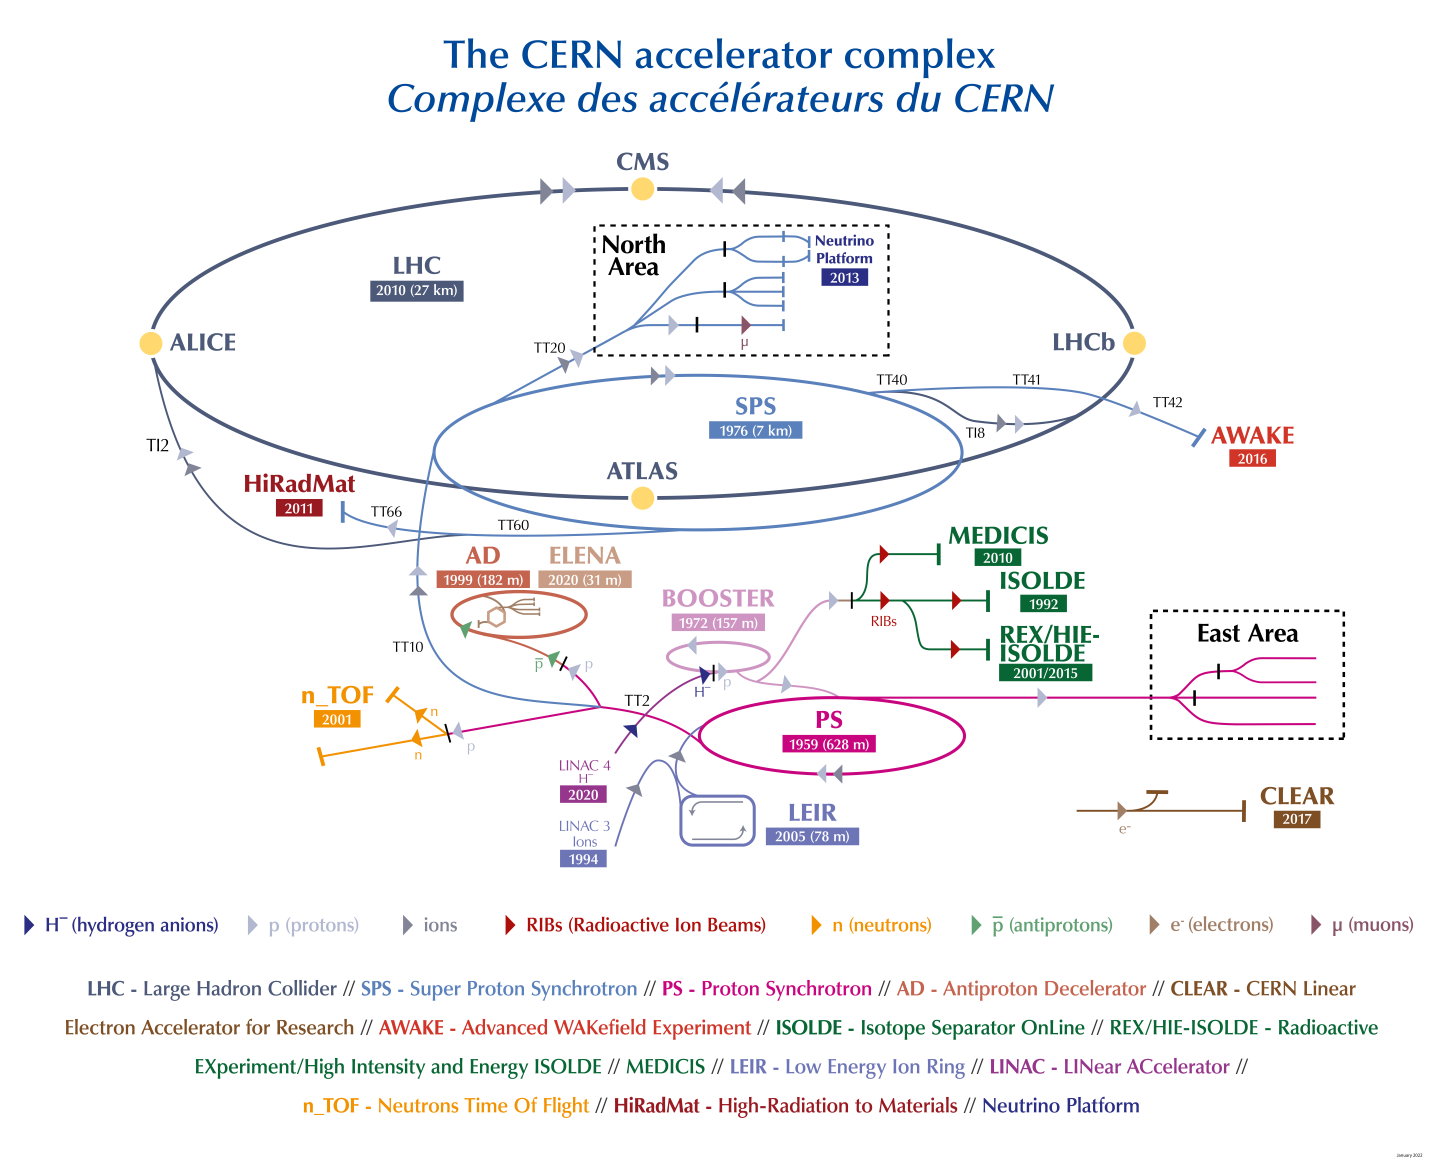
\includegraphics[width=1\textwidth]{images/introduction/cern_accelerator_complex.png}
        \caption{Schematic view of the CERN accelerator complex. The different colors correspond to the different machines. The year of commissioning and the type of particles used in each one of them are also indicated along with the circumference for the circular machines. The image is courtesy of CERN~\cite{Lopienska:2800984}.}
        \label{fig:cern_accelerator_complex}
 \end{figure}

 It is worth mentioning that not only protons but also lead ions are accelerated in the LHC, starting their journey from Linac3 and Low Energy Ion Ring (LEIR) and then in PS and SPS as proton beams.

 Finally, the accelerators in the injector chain not only prepare the beam for the LHC but also provide beams to various other facilities and experiments at lower energies. Examples are the Anti-proton Decelerator (AD) which studies antimatter, the Online Isotope Mass Separator (ISOLDE) which studies the properties of the atomic nuclei using radioactive beams, and the Advanced Proton Driven Plasma Wakefield Acceleration Experiment (AWAKE) which investigates particle acceleration by proton-driven plasma wakefields.

 \subsection{The CERN Super Proton Synchrotron}\label{subsec:cern_sps}
 % sps history: https://be-dep-op-sps.web.cern.ch/history
 The research described in this thesis was conducted at the Super Proton Synchrotron (SPS) and some additional information about this machine is provided here. The SPS (shown with light blue color in Fig.~\ref{fig:cern_accelerator_complex}) was first commissioned in 1967 and has a circumference of 6.9\,km. It used to operate as a proton-antiproton collider ($\mathrm{Sp\bar{p}S}$) and later on as an injector for the Large Electron Positron collider (LEP) while it also provided beams for fixed-target experiments (e.g. in the North Area). Even though the SPS can accelerate various particle types (protons, antiprotons, electrons, and heavy ions) the following information will concern its operation with proton beams which is the topic of the research presented in this thesis.

 Currently, the SPS is the second biggest accelerator at CERN and it can accelerate protons up to 450\,GeV. Due to its past use as a collider, it can also operate as a storage ring. This operational mode is called "coast" and was used for the majority of the experimental studies presented in this thesis. During coast, the bunches circulate in the machine for long periods at constant energy. The highest energy at which SPS can operate in coast is 270\,GeV due to limited cooling of the magnets to transfer away the heat when operating at high energy and consequently at large currents for long periods.

 %After that they are injected in the LHC. Hoewever, as it used to be a collider it can operate as a storage ring, it is called coast (des ti exeis grapsei.) and will be used for the studies in this thesis.
 

\section{High-Luminosity LHC project and Crab Cavities}
%LHC is the flagship of the CERN accelerator complex and is the at the cutting edge of the accelerator and high energy physics research with almost ten thousand scientists working for and with it. In order to extend its discovery potential LHC will undergo a major upgrade in the coming years. 
% Hl-lhc book: p.2 hl-lhc is the top priority of the european strategy of particle physics. 
High-Luminosity LHC (HL-LHC)~\cite{HL_LHC_yellow_report, Brning2015} is the upgrade of the LHC machine which will extend its potential for discoveries. In particular, it aims to increase the instantaneous luminosity by a factor of 5 beyond the current operational values and the integrated luminosity by a factor of 10. 

The luminosity, along with the energy, is a key parameter defining the performance of a collider as is a measure of the collision rate. The instantaneous luminosity is expressed as~\cite{luminosity}:

\begin{equation}\label{eq:luminosity_inst}
    \mathcal{L} = \frac{n_b f_\mathrm{rev}N_1 N_2}{4 \pi \sigma_x \sigma_y} \frac{1}{\sqrt{1+(\frac{\sigma_z}{\sigma_\mathrm{xing}} \frac{\theta_c}{2})^2}},
\end{equation}

where $f_{\mathrm{rev}}$ is the revolution frequency of the machine (the number of times per second a particle performs a turn in the accelerator, definition; in Chapter~\ref{Ch:theory}), $n_b$ is the number of colliding bunch pairs, $N_{1,2}$ is the number of particles per bunch, $\sigma_{x,y}$ is the transverse beam size at the interaction point, $\sigma_z$ the rms bunch length, $\sigma_{\mathrm{xing}}$ the transverse beam size in the crossing plane and $\theta_c$ is the full crossing angle between the colliding beams. % Andy's comment: use "number of particles per bunch" instead of "bunch intensity" which is slightly ambiguous.
 The crossing angle, is often introduced between the bunches in a collider to reduce parasitic collisions and get rid of the remnants after the collision. For reference, in the LHC, the crossing angle has order of magnitude $10^{-4}$ radians. % hundreds of micro radians, see sofia's thesis Table 4.4 for example. https://cds.cern.ch/record/2743602/files/CERN-THESIS-2020-169.pdf

The integrated luminosity is the one that ultimately defines the performance of the machine as it provides the total number of recorderd events. It depends both on the instantaneous luminosity and on the machine availability. The integrated luminosity, is expressed as~\cite{HL_LHC_yellow_report}:
\begin{equation}\label{eq:integrated_luminosity}
    \mathcal{L}_I \equiv \int_{\Delta t} \mathcal{L} dt,
\end{equation}

where $\mathcal{L}$ is the instantaneous luminosity as defined in Eq.~\eqref{eq:luminosity_inst}.
% for more details and specific values check sofias thesis.
% and: https://accelconf.web.cern.ch/ipac2015/papers/thxb2.pdf

HL-LHC aims to achive instantaneous luminosity of $\mathcal{L} \sim 5 \cdot 10^{34} \ \mathrm{cm^{-2} s^{-1}}$ and an increase on the integrated luminosity from 300 $\mathrm{fb^{-1}}$ to 3000 $\mathrm{fb^{-1}}$ over its lifetime of 10-12 years and considering 160 days of operation per year~\cite{Brunning_Rossi}. % 160 days. p.. 80 in the reference
% The integrated luminosity for both lhc and hl-lhc is over 10-12 years.

% 160 days of physics events per year:https://cds.cern.ch/record/2031207/files/198-201_Fessia.pdf

% Source v2: https://accelconf.web.cern.ch/ipac2019/papers/mopgw095.pdf

%\normalsize{\textbf{Crab Cavities}}\\
\subsection{Crab cavities}\label{subsec:CC_intro}
To achieve its luminosity goals, HL-LHC will employ numerous innovative technologies. Crab cavity technology (will be denoted as $\CC$ in this thesis)~\cite{Calaga:2673544} is one of the key componenets of the project as it will be employed to restore the luminosity reduction caused by the crossing angle, $\theta_c$ (see Eq.~\eqref{eq:luminosity_inst}).

A crab cavity is an RF cavity which provides a transverse, sinusoidal like, kick to the particles depending on their longitudinal position within the bunch. A graphical visualisation of the kick is shown in Fig.~\ref{fig:cc_simple_kick}. It can be seen that the head (leading part) and the tail (trailing part) of the bunch receive opposite deflection while the particles at the center remain unaffected.

\begin{figure}[!h] % at the directory of ipac22
    \centering         
    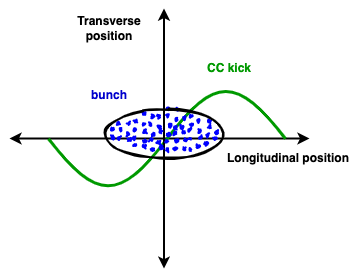
\includegraphics[width=0.5\textwidth]{images/introduction/sin_CC_kick_LHC_beams.drawio.png}
        \caption{Visualisation of the CC kick (green line) on the bunch particles (blue dots). The bunch here appears much smaller than the CC wavelength which means that only the linear part of the kick affects the bunch. This will be the case for the HL-LHC scenario.}
        \label{fig:cc_simple_kick}
 \end{figure}

The $\CC$s will be installed in the two main interaction points of LHC, ATLAS and CMS. According to the plan, two $\CC$s will be installed on each ring and on each side of the interaction points (eight in total). This is displayed in Fig.~\ref{fig:LHC_layout_CCs} with the red (ATLAS) and orange (CMS) markers. The reason why two $\CC$s are needed in each ring on each side of the IP is discussed in the following paragraphs (local vs global scheme).

\begin{figure}[!h] % made at diagrams.net saved at google docs
    \centering         
    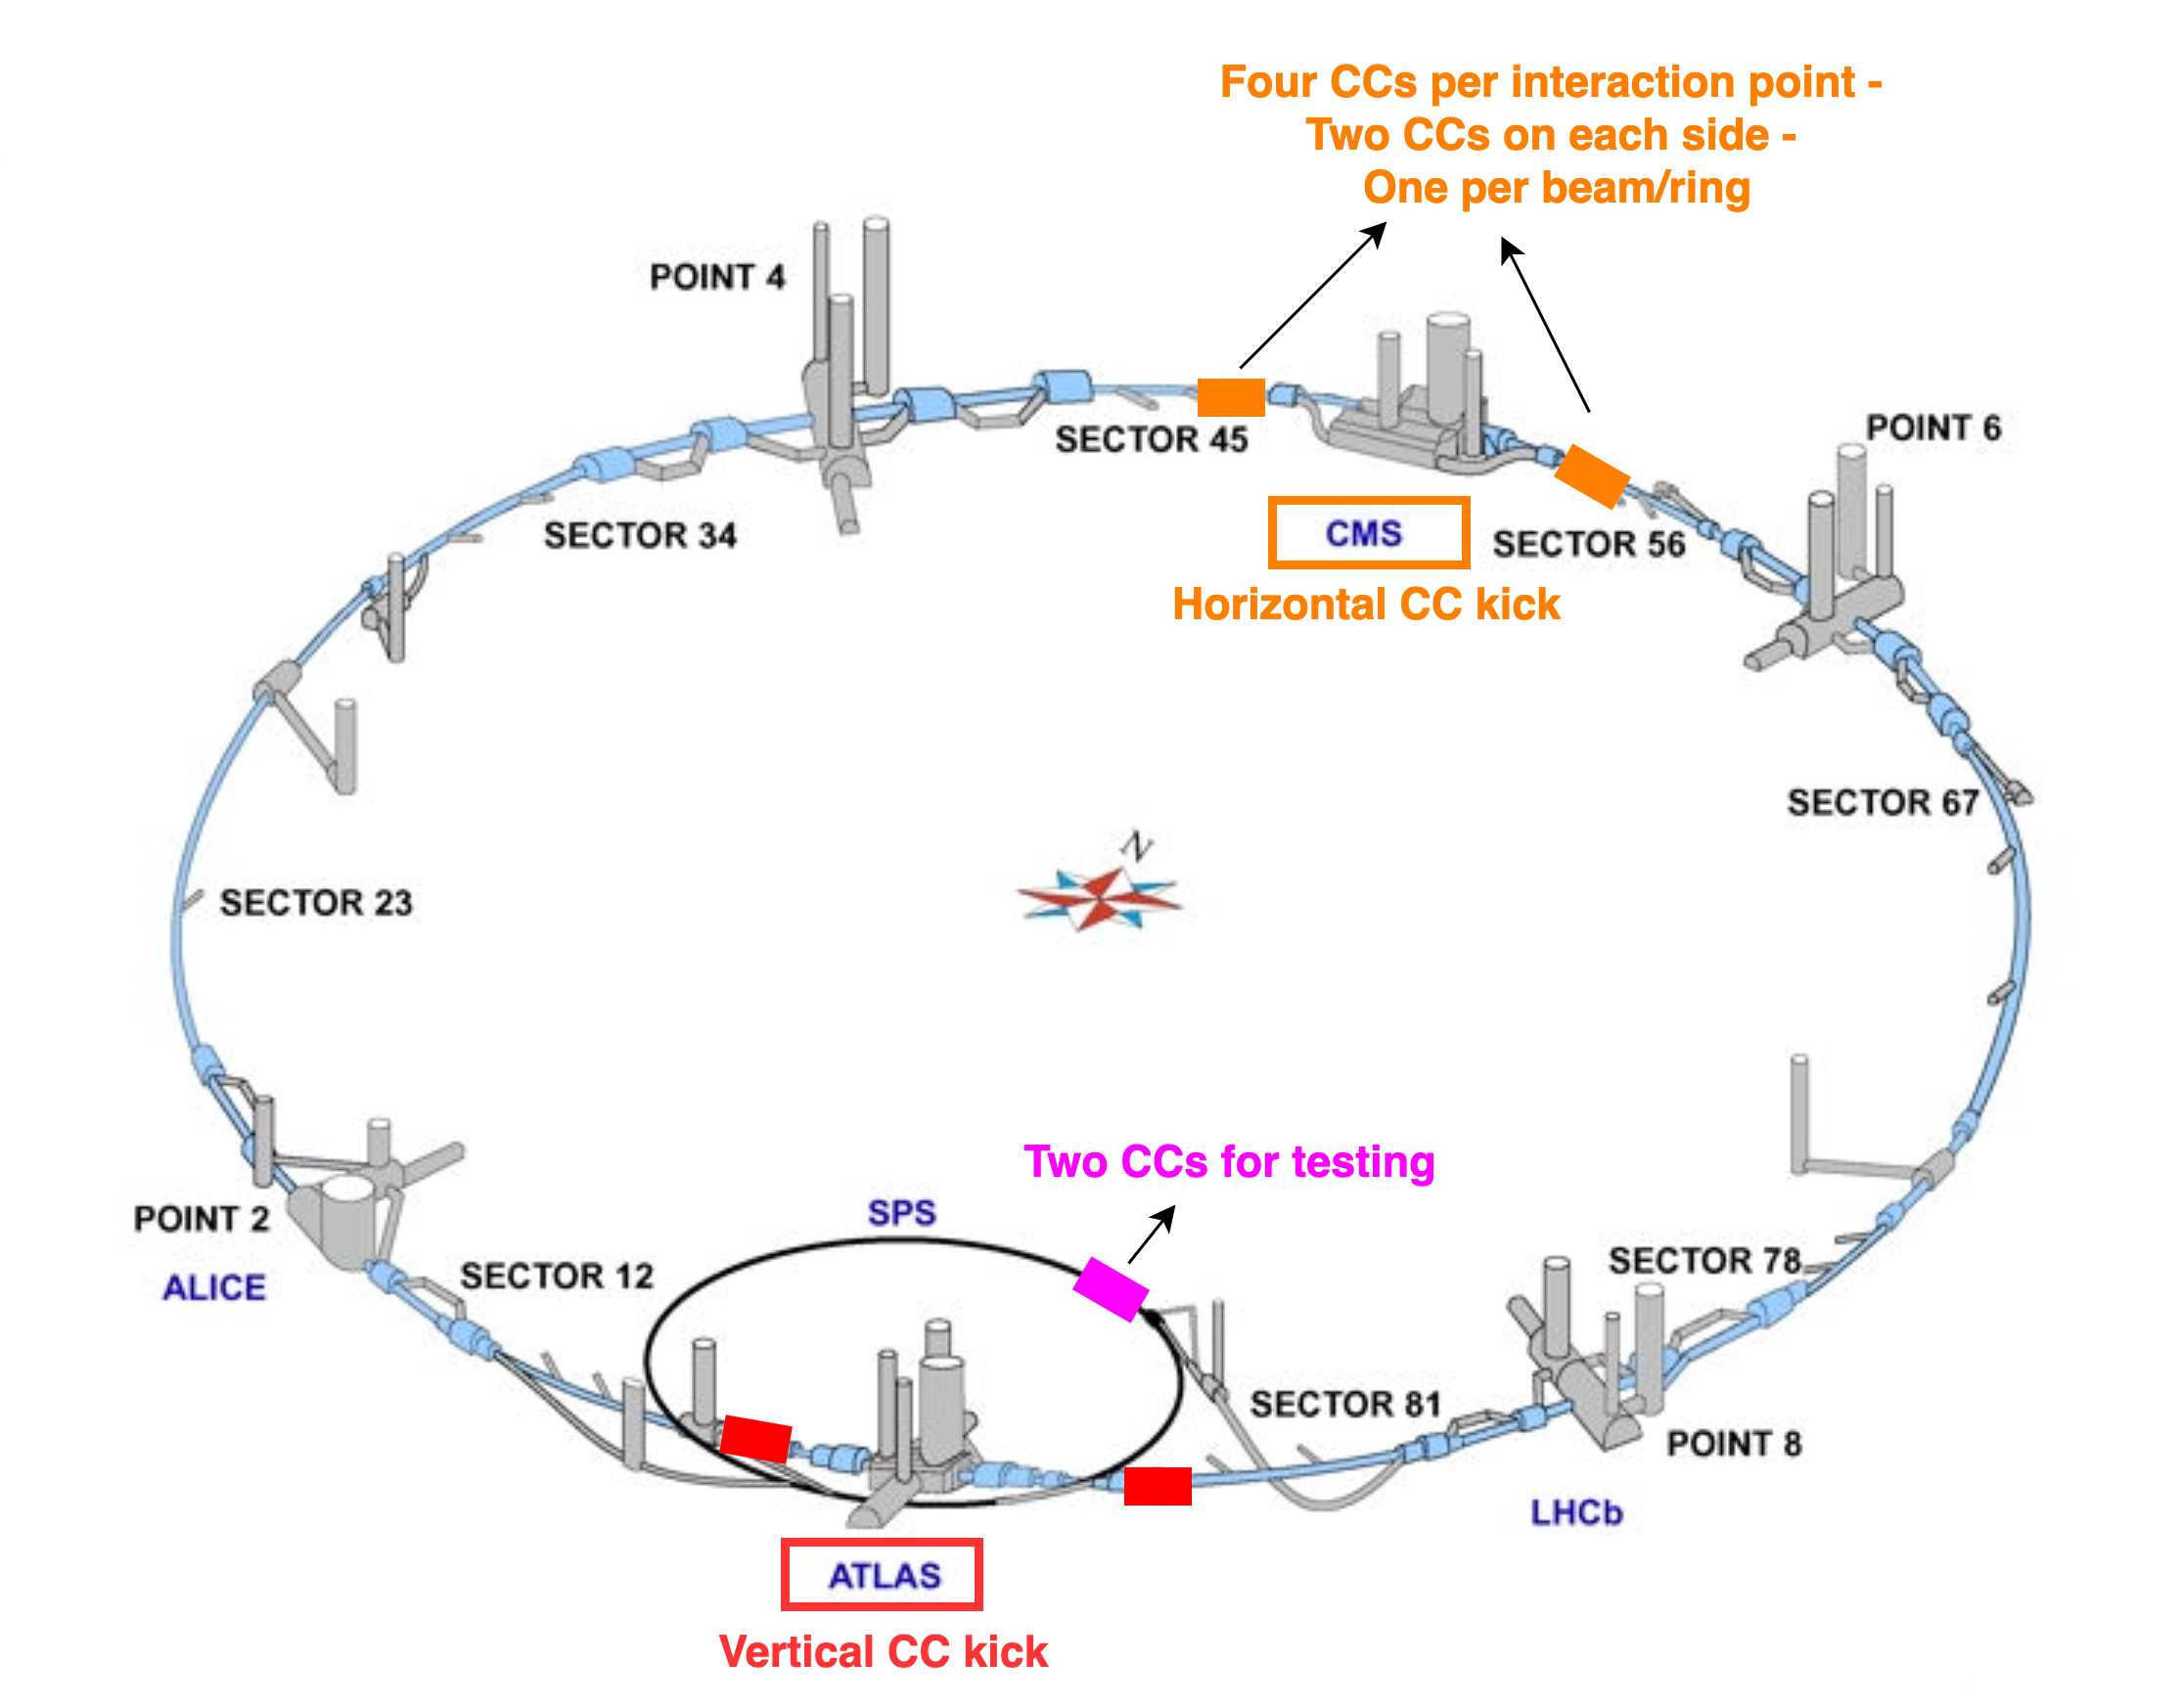
\includegraphics[width=0.8\textwidth]{images/introduction/LHC_layout_CCs.png}
        \caption{Layout of the LHC and the SPS. The CC location for the HL-LHC configuration is marked. Two CCs (one per ring) will be installed on each side of ATLAS (red) and CMS (orange). Two protoype CCs were also installed in the SPS (magenta) in 2018, to be tested before their installation in LHC. The layout can be found in Ref.~\cite{LHC_SPS_layout} and was modified inspired by Ref.~\cite{LHC_SPS_layout_v2}.}
        \label{fig:LHC_layout_CCs}
 \end{figure}

In this configuration, the bunches receive the transverse deflection from the first pair of $\CC$s just before reaching the interaction point. This results in a rotation of the bunch, which mitigates the crossing angle and restores the head-on collisions. The deflection is cancelled once the bunches reach the second pair of $\CC$s which are symmetrically placed at the opposite side of the interaction point. The collision of the bunches in the presence of the $\CC$s is illustrated in Fig.~\ref{fig:crossing_with_and_without_CCs}~\cite{Verdú-Andrés:2263119}.
% 90 deg between CCs and IP. https://cds.cern.ch/record/2263119/files/10.1016_j.nuclphysbps.2015.09.025.pdf

\begin{figure}[!ht]
    \centering
    \begin{subfigure}[t]{0.45\textwidth}
        \centering
        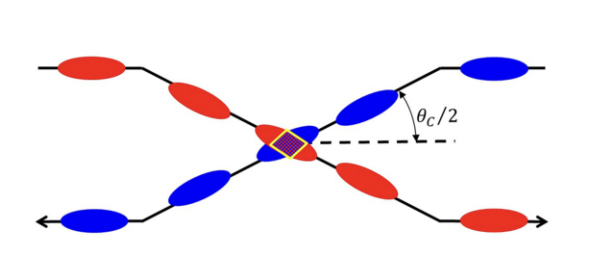
\includegraphics[width=1\textwidth]{images/introduction/no_crab_crossing.png}
        \caption{Crossing without CCs}
        %\label{fig:add_label_here}
    \end{subfigure}
    \hfill
    \begin{subfigure}[t]{0.45\textwidth}
        \centering
        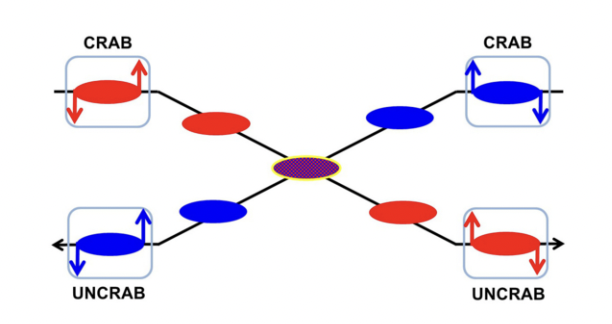
\includegraphics[width=1\textwidth]{images/introduction/crab_crossing.png}
        \caption{Crossing with CCs}
        %\label{fig:add_label_here}
    \end{subfigure}
    \hfill
     \caption{Collision with and without the use of CCs~\cite{Verdú-Andrés:2263119}. CCs restore the overlap between the bunches recovering the luminosity reduction caused by the crossing angle, $\theta_c$. The blue and red colors indicate indicate two bunches in the different rings.} 
     \label{fig:crossing_with_and_without_CCs}
 \end{figure}


% Local vs global CC scheme: https://slideplayer.com/slide/10896302/ 
The above scheme, with $\CC$s before and after the interaction point, is called the local crabbing scheme. An alternative scheme, named the global crabbing scheme, was also under discussion in the first stages of the project. In such as scheme, the closed orbit distortion that is caused by the fact that the head and the tail of the bunch are kicked in opposite directions propagates in the ring, resulting in transverse bunch oscillations~\cite{Brning2015}. This scheme is cost-efficient compared to the local scheme as it only requires two CCs. However, it introduces significant constraints on the betatron phase advance between the interaction points and the CCs. The constraints are enhanced by the fact that the bunch crossing in ATLAS takes place in the vertical plane while in CMS in the horizontal. To this end, the local $\CC$ scheme was chosen for the HL-LHC configuration. % uncrabbing.
%HL-LHC book p.138: The transverse kick introduced by this cavity, different  for  the  head  and  the  tail  of  each  bunch,  is  equivalent  to  a  closed  orbit  distortion, i.e. head and tail would follow their individual closed orbit around the ring, their tilt wobbling around the unperturbed closed orbit of the bunch center.

In order to accommodate the crossing in both transverse planes two $\CC$ designs have been developed: the Double-Quarter Wave (DQW) and the RF dipole (RFD), which provide vertical and horizontal deflection respectively. Information on their design can be found in Refs.~\cite{Zanoni:2288282, DeSilva:2288607, Xiao:1992565, Verdú-Andrés:2113440}

% short summary about KEKB in sylivias paper: https://cds.cern.ch/record/2263119/files/10.1016_j.nuclphysbps.2015.09.025.pdf
The $\CC$s have already been successfully used in the KEKB collider~\cite{Toge:475260} in Japan, during 2007-2010, with lepton beams ($e^{+} - e^{-}$)~\cite{CC_KEKB_4440798, Funakoshi:1955812, oide:pac07-mozaki01}. However, there are significant differences in the beam dynamics in the presence of $\CC$s in leptons and hadrons (HL-LHC case). One of the most crucial points is the impact of errors (e.g. RF noise) which leads to beam degradation~\cite{Calaga:2773279, Alekou:2696109}. This is not an issue of concern for lepton beams as they nevertheless experience emittance damping due to synchrotron radiation. For proton beams, the synchrotron radiation damping is much weaker meaning that the beam degradation can lead to emittance growth which eventually can result in loss of luminosity. % Andy's comment: "emittance damping" would be better than "beam-size damping". 

% other crabbing errors: phase and amplitude rf noise, wakefields (Calaga)
% other difference between letptons and protons (protons: much longer bunches)

% Potential questions to answer for the CC test.
%https://indico.cern.ch/event/800428/attachments/1804664/2945632/CrabCavity_BE_Seminar.pdf
As the $\CC$s have never been used with protons before, two prototype superconducting $\CC$s were installed in the SPS (Fig.~\ref{fig:LHC_layout_CCs}, magenta markers) to test the technical systems, to validate their operation with proton beams and to identify and address potential issues before their installation in LHC. The SPS  provides an ideal test bed for these studies as it allows testing under conditions that are closer to those in HL-LHC than any other machine. In particular, the SPS operates with proton beams, can run in storage-ring mode, and in terms of the energy reach is second only to LHC. The two $\CC$s that were installed in SPS~\cite{Zanoni:2017} were identical, fabricated at CERN and of the DQW type (like the ones that will be used in ATLAS interaction point in HL-LHC).


\section{Motivation, objectives and thesis outline}\label{sec:motivation_outline}

As mentioned above, one of the main concerns regarding the $\CC$ operation with protons is the emittance growth due to noise in their RF system as it leads to luminosity loss. For the HL-LHC, the target values regarding the luminosity loss and emittance growth are very tight. In particular the maximum allowed luminosity loss due to $\CC$ RF noise induced emittance growth is targeted at just 1$\%$, during a physics fill, which corresponds to an $\CC$ RF noise induced emittance growth of 2 $\mathrm{\%/h}$~\cite{MedinaMedrano:2301928, CC_lumi_limits_philippe, CC_lumi_limits_ilias}. To this end, a good understanding and characterization of the emittance growth mechanism is crucial for the HL-LHC project.

For reference, a physics fill is the time period during which the beams are successfully injected in the LHC at the desired conditions, they are accelerated at the desired energy and they are kept in the machine for consectuive collisions. After some hours, due to beam degradation the beams are dumped and a new fill is prepared. A fill in the HL-LHC will lasts a couple of hours. 

The main objective of this thesis is to understand, characterise and evaluate the mechanism of $\CC$ RF noise-induced emittance growth including numerical and experimental studies. The studies presented in this thesis were conducted for the SPS machine since it has proton crabbing operational experience and allows direct comparison of predictions from models and experimental data. It should be emphasised that the CC tests in SPS constitute the first experimental beam dynamics studies with $\CC$s and proton beams. The results and the understanding obtained from this research are essential for the HL-LHC, in order to predict the long-term emittance and to define limits on the acceptable noise levels for the $\CC$s.
%and for the design of the crab cavity HL-LHC Low-Level RF system.
% the outcome is that the dedicated damper is necessary. possibility to integrate at the ADT.

This thesis reports research that was carried out between 2018 and 2022, based at CERN and it stractured as follows:

Chapter~\ref{Ch:theory} presents the basics of accelerator beam dynamics focusing on the concepts that are relevant for understanding the studies presented in this thesis. In particular, definitions are given for single-particle beam dynamics, addressing both transverse and longitudinal motion. Furthermore, the collective effects are introduced focusing on the effect of wakefields. A brief discussion on optics models for accelerators is also provided. Finally, the two simulation codes used in this thesis for macroparticle tracking, PYHEADTAIL, and Sixtracklib, are described.
% see sondre's thesis.

The available theoretical model, developed by T.~Mastoridis and P.~Baudrenghien~\cite{PhysRevSTAB.18.101001}, for predicting the emittance growth driven by Crab Cavity RF noise is described in Chapter~\ref{Ch:CC_noise_theory}. This model will be referred to as Mastoridis--Baudrenghien model or theory throughout the thesis. The modeling of the noise effects in the simulations is also discussed. Last, a short reference to the CC experiment at KEKB in Japan is also made. 

Chapter~\ref{Ch:2018_analyisis} is devoted to the results of the first experimental studies of the emittance growth from $\CC$ RF noise in the SPS. First, the experimental configuration and procedure are reported. Second, the artificial noise injected in the $\CC$ RF system for the measurements is discussed in detail. Subsequently, the emittance growth measurements are presented along with the measured bunch length and intensity evolution for completeness. Last the measured emittance growth rates are compared with the predictions from the Mastoridis--Baudrenghien theory. It was found the measured growth rates were systematically a factor of 4 on average lower than the predictions. 

Various possible factors were investigated as a possible explanations for this discrepancy. These extensive studies are described in Chapter~\ref{Ch:investigating_discrepancy}. Initially, parametric studies based on the theoretical model studied the sensitivity of the $\CC$ RF noise-induced emittance growth to possible uncertainties in the CC voltage amplitude and bunch length. The theory was also benchmarked with different simulation software: PyHEADTAIL and Sixtracklib. The sensitivity of the emittance evolution on the non-linearities of the SPS machine (which is not included in the Mastoridis--Baudrenghien theory) was also tested. Finally, thorough studies were performed to exclude the possibility that the discrepancy is not a result of the z-dependent orbit shift induced by the $\CC$ kick or the actual noise spectra applied on the $\CC$s. However, none of these factors could explain the discrepancy.

Finally, simulations including the SPS transverse impedance model (not included in the theory (of Chapter~\ref{Ch:CC_noise_theory}) showed a significant impact on the emittance growth. Chapter~\ref{Ch:suppression_impedance} discusses the investigation and characterisation the phenomenon of the emittance growth suppression from the beam coupling impedance as observed in simulations with PyHEADTAIL. It was shown that the suppression is related to the dipole motion which is excited by the $\CC$ RF phase noise.

Chapter~\ref{Ch:experimental_CC_2022}, presents the results from the experimental studies that took place in the SPS in 2022. The objective of this experimental campaign was to validate the mechanism of the suppression of the $\CC$ RF noise-induced emittance growth from the beam coupling impedance as observed in simulations (described in Chapter~\ref{Ch:suppression_impedance}). This would also confirm that this impedance-induced effect is the reason for the discrepancy observed in the 2018 experiment between the measurements and the Mastoridis--Baudrenghien theoretical predictions. Despite the challenging conditions of the studies, the experiments of 2022 successfully confirmed the emittance growth suppression mechanism, despite the very challenging conditions of the studies.

%presents the results from the second round of emittance growth measurements with $\CC$s in SPS that took place in 2022. The objective of these experimental studies was to validate the mechanism of the suppression of the $\CC$ RF noise-induced emittance growth from the beam coupling impedance as observed in simulations (described in Chapter 7). This would also confirm that this impedance-induced effect is the reason for the discrepancy observed in the 2018 experiment between the measurements and the theoretical predictions. The experiments of 2022 successfully confirmed the suppression mechanism, despite the very challenging conditions of the studies.

Last, Chapter~\ref{Ch:conclusions} summarizes the conclusions of the thesis. The project is viewed from a broad persepective highlighting its importance for the HL-LHC project. Potential follow up studies are proposed.

\chapter{Basics of accelerator beam dynamics}
The definitions and notations used throughout this thesis are based on the book of A. Wolksi in Ref.~\cite{wolski2014} unless it is stated otherwise. In this chapter, the basic concepts of accelerator beam physics that are essential for understanding the studies presented here are introduced. The focus is put on the concepts for synchrotrons with proton beams. Additionally, in the last section, the tracking simulation codes used in this work are described.

% Details p.11 Michael schenk
Synchrotrons are circular accelerators where the particles follow a fixed closed-loop path. In a synchrotron, electric fields accelerate the particles while magnetic fields steer and focus them. The magnetic fields are not constant but they vary according to the particles' energy, allowing acceleration and operation in very high (relativistic) energies. The LHC and SPS machines at CERN are synchrotrons like the most of the machines used for High Energy Physics experiments. Usually, in synchrotrons, the beams consist of multiple bunches, longitudinally spaced around the machine, which of course interact with each other. However, these multi-bunch interactions are not relevant to the studies presented in this thesis. Therefore, they are not addressed in the following paragraphs. 

% section splitting accordin to Wolski.
\section{Motion of charged particles in electromagentic fields}
The motion of a particle with charge $q$ and velosity $\mathbf{v}=(v_x, v_y, v_z)$ moving in an electric field $\mathbf{E}$ and a magnetic field $\mathbf{B}$ is defined by the influence of the Lorentz force: 
\begin{equation}\label{eq:Lorentz_force}
    \mathbf{F} = q(\mathbf{E} + \mathbf{v} \times \mathbf{B}).
\end{equation}
% v is tangential to its path.

At this point, it is appropriate to mention that in this thesis the vectors are denoted in bold font (e.g. $\mathbf{E}$ ). % For the relativistic and ultrarelativistic regime the impacrt of E and B are the same. E = cB. p.44 Wille

In synchrotrons, the electric fields, which are generated by Radiofrequency (RF) cavities, are used for accelerating the beams. The magnetic fields, are used to steer (dipoles) and focus (quadrupoles) and apply corrections (sextupoles, octupoles and higher order multipoles) at the motion of the beam.

\textbf{Reference trajectory and reference particle}\\
The sequence of the various electromagnetic elements around the accelerator ring is called the machine lattice. The ideal path that passes through the center of all the magnets is called the design orbit or the reference trajectory. This reference trajectory (red line Fig.~\ref{fig:coordinate_system}) has circumference $C=2\pi R$ (where $R$ is the radius of the ring) and is predetermined by the construction of the accelerator. 

The particle that follows this trajectory is called the reference particle and has a momentum $p_0$, an energy $E_0$, and a velocity $v_0$. This particle is often called the synchronous particle as it always passes from the center of the RF cavities (assuming constant speed and no losses). %https://indico.cern.ch/event/22574/contributions/475143/attachments/371243/516589/IntroductionToAccelerators.pdf slide 36
For a proton, the reference momentum is given by: $p_0 = \gammarel m_0 v_0$, where $m_p$ is the proton rest mass.

\textbf{Mangetic rigidity}\\
At this point, it is appropriate to introduce the concept of magnetic rigidity, $B_0 \rho$, which is often used in accelerators as a normalisation factor and is a measure of how the charged particles resist bending by a dipolar magnetic field. Assuming that a proton moves only under the influence of a uniform vertical dipole field $\mathbf{B_0}=(0, B_0, 0)$, it would follow a circular path of radius $\rho$ which is defined by the Lorentz force (Eq.~\eqref{eq:Lorentz_force}) being equal to the centripetal force, as follows:

\begin{equation}\label{eq:Brho}
    e v_0 B_0 = \frac{\gammarel m_p v_0^2}{\rho} \Rightarrow B_0 \rho = \frac{\gamma_0 m_p v_0}{e} \Rightarrow B_0 \rho = \frac{p_0}{e},
\end{equation}
where $e$ and $m_p$ are the charge and rest mass of a proton respectively, $p_0$ is the reference momentum, and $\gammarel = \frac{1}{\sqrt{1-\beta^2}}$ is the relativistic gamma or Lorentz factor, where $\betarel=v_0/c$ is the relativistic $\beta$ with $c$ being the speed of light. In the ultra-relativistic regime which is the case in the studies presented in this thesis, $\betarel=1$.
% IMPORTANT!!! -->  v_0 = v_z. You explain this in the next paragraph.

If the particle momentum is given in $\mathrm{GeV /c}$ (usuall units in high energy accelerators) then the unit of magnetic rigidity is $\mathrm{T \cdot m}$. 

%- https://uspas.fnal.gov/materials/12MSU/xverse_dynamics.pdf

\textbf{Co-ordinate system}\\
However, the individual particles do not follow the reference trajectory due to small deviations in their initial conditions: an example trajectory is shown in Fig.~\ref{fig:coordinate_system} with the blue line. The co-ordinate system used to describe the individual trajectories of the beam particles around the accelerator is illustrated in Fig.~\ref{fig:coordinate_system} and it is known as Frenet-Serret system.  It consists of the orthogonal co-ordinate system $\Sigma(s) = (\mathbf{e_x}, \mathbf{e_y}, \mathbf{e_z})$ whose origin moves along the reference trajectory (red line) together with the beam. 

The variable $s$ denotes the distance along the reference trajectory. In accelerator physics, $s$ is usually chosen as the independent variable instead of time, $t$.  %why? p.19 https://www.bnl.gov/isd/documents/74289.pdf
Therefore, at any given location $s$ around the ring, the coordinates $(x(s), y(s), z(s))$ give the horizontal, vertical, and longitudinal position of the particle with respect to the origin of the orthogonal moving system $\Sigma$. In the following paragraphs, the dependence of the co-ordinates on the position $s$ along the ring is omitted when possible to facilitate the notation (e.g. x(s) will be denoted as x).

\begin{figure}[!h] % at the directory of ipac22
    \centering         
    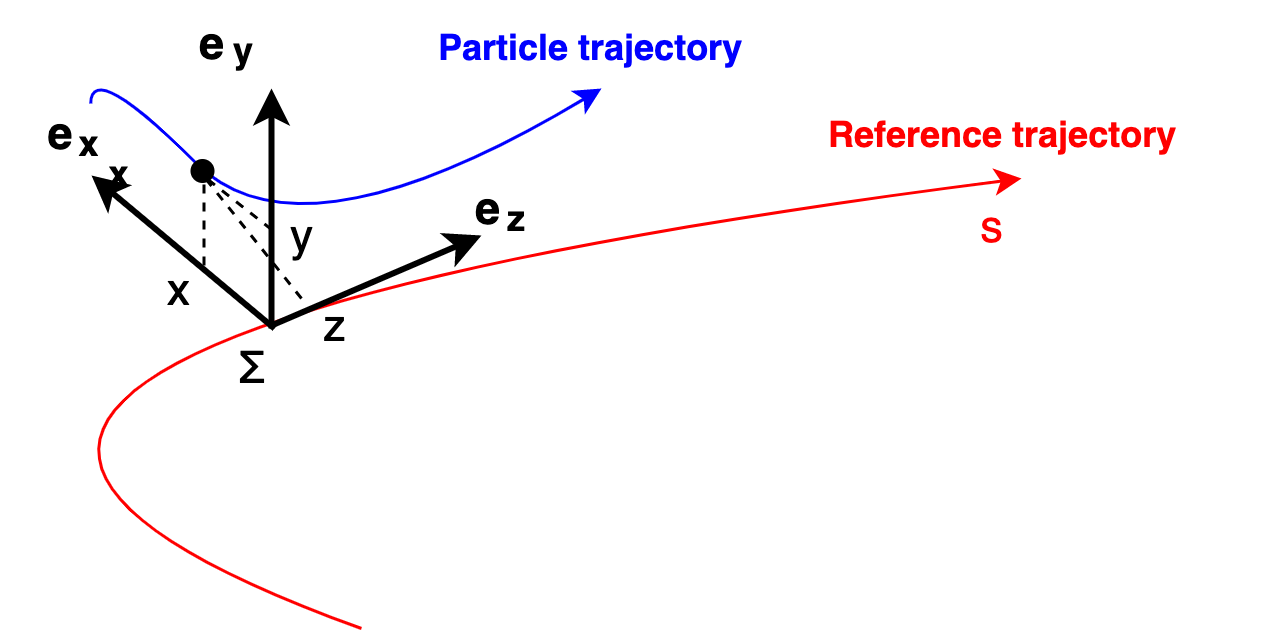
\includegraphics[width=0.8\textwidth]{images/Ch2/coordinates_particle_motion.png}
        \caption{Co-ordinate system used to describe particles motion in a synchrotron. This is a rotating co-ordiante system, with $(\mathbf{e_x, e_y, e_z})$ being the unit vectors, which follows the reference trajectory along the accelerator.}
        \label{fig:coordinate_system}
 \end{figure}


 At any point $s$ along the reference trajectory each particle is represented by the following 6-dimensional vector $(x, x^{\prime}, y, y^{\prime}, z, \delta)$ where:

 \begin{subequations}\label{eq:particle_coordinates}
    \begin{equation}
        x^\prime = \frac{dx}{ds} = \frac{dx}{dt}\frac{dt}{ds} = \frac{v_x}{v_z} =  \frac{p_x}{p_z} \approx \frac{p_x}{p_0},
    \end{equation}    
    \begin{equation}
        y^\prime = \frac{dy}{ds} = \frac{dy}{dt}\frac{dt}{ds} = \frac{v_y}{v_z} =  \frac{p_y}{p_z} 	\approx \frac{p_y}{p_0},
    \end{equation} 
    \begin{equation}
        \delta = \frac{\Delta p}{p_0} = \frac{p-p_0}{p_0},
    \end{equation}
    \begin{equation}
        z = \betarel c (t_0 -t),
    \end{equation}
\end{subequations}

where $p_0$, $\beta_0$ is the momentum of the reference particle and the relativistic $\beta$ as defined in the previous paragraph, $t_0$ is the time  which the reference particle arrives at the location $s$ and $t$ is the time at which the individual particle arrives at the same locaiton. It can be seen, that $\delta$ is the relative momentum offset from the reference particle. In order to avoid a possible misconception it seems appropriate to clarify here, that the longitudinal parameter $z$ indicates the longitudinal offset from the reference particle at the center of the bunch. If $z>0$ ($z < 0$) the corresponding particle reaches earlier (later) than the center of the bunch at an arbitrary reference point. Last, in the ultra-relativistic regime the momentum of the particles in the $\mathbf{e_z}$ direction is much larger than the transvserse ones and almost equals the reference momentum: $p_x, p_y \ll p_z = p_0$. This is why, the $x^\prime$ and $y^\prime$ are basically the normalised momentum with the reference one, $p_0$.

%Furthermore, if the direction of motion of the particle has a small angle with the reference trajectory, the paraxial approximation is valid: $p_x, p_y \ll p_z = p_0$ which means that $x^\prime \approx p_x$ and  $y^\prime \approx p_y$. This approximation is valis for the studies presented in this thesis. \textcolor{red}{$p_0=1$? not clear to me} % ultra relativistic regime, is not mentioned at wolski's book. I wrote it for the p_ 0= 1. but i am not sure.
% p.149 wolski and p.12 Michael schenk

%is the momentum of the reference particle which is given by: $p_0 = \gammarel m_0 v_0$, where $m_0$ is the proton rest mass and
%It can be seen that $x^\prime$ and $y^\prime$ are basically the normalised momenta with the reference momentum $p_0$ and $\delta$ is the relative momentum offset from the reference particle. 

%Initial I have written: Furthermore, the ultra-relativistic regime, the transverse momentum/velocity of a particle is very small comparing to the longitudinal one. Therefore the paraxial approximation is used: $p_x, p_y \ll p_z = p_0 = 1$ which can be applied to simplify Eqs.~\ref{eq:particle_coordinates}. %Or see Andy's explanation for low emittance storage rings: https://cds.cern.ch/record/1982424/plots

To summarize, the motion of the particles is separated in the transverse and longitudinal planes where it is described with the  $(x, x^\prime, y, y^\prime)$ and $(z, \delta)$ co-ordinates respectively. As an example the co-ordinates of the reference particle are $(x=0, x^\prime=0, y=0, y^\prime = 0, z=0, \delta=0 \ (p_z=p_0))$.

\section{Single-particle beam dynamics}
In this first section, the interactions between the particles within a bunch are neglected, hence the term single-particle beam dynamics.

\textbf{Two-dimensional complex fields}\\
As already discussed, the motion of the charged particles inside a circular accelerator is controlled by magnetic fields. In this thesis, the magnets are considered purely transverse elements. Their effect is therefore described with two-dimensional multipole fields, acting in the horizontal and vertical planes\footnote{Examples of three-dimensional treatment can be found in~\cite{wolski2014, Beth:889480}. However, the two-dimensional treatment is most often used in accelerator physics as it provides a good description for the majority of the magnetic elements.}. % Wolski Ch1.3, p.33

The description of two-dimensional magnetic fields in accelerator physics is discussed using the concept of multipole expansion and is expressed as a complex quantity. The complex quantity it allows to describe a two-dimensional field in $(x,y)$ space (to be compatible with the co-ordinates used for describing the particle's trajectory as discussed in the previous section). Therefore, the magnetic field around the beam is expressed as follows~\cite{wolski2014}: 
\begin{equation}\label{eq:mult_expansion} % Andy Eq.1.29 + M Schenk Eq.2.2
    B_y(x,y) + i B_x(x,y) = \sum_{n=1}^{\infty} C_n (x+i y)^{n-1},
\end{equation} % principle of superposition 
where $n$ indicates the order of the field component: $n$=1 for a dipole (steering), $n$=2 for quadrupole (focusing (chromticity correction), $n$=4 for octupole (error or field correction) etc. $C_n=(b_n +i \alpha_n)$ is a complex constant which denotes the strength and orientation of the multipole field. The coefficients $b_n=\frac{1}{(n-1)!} \frac{\partial^{n-1}B_y}{\partial x^{n-1}}$ and $\alpha_n=\frac{1}{(n-1)!} \frac{\partial^{n-1}B_x}{\partial x^{n-1}}$ denote the strength of a normal and skew (normal multipole rotated by $\pi/2(n-1)$) multipole respectively in units of $\mathrm{T/m^{n-1}}$.
% Equations for coefficients, sofia's thesis Eq.(2.29) p. 23: https://cds.cern.ch/record/2743602/files/CERN-THESIS-2020-169.pdf

Usually, in accelerator physics the values of the multipole strengths are quoted normalised to the magnetic rigidity as defined in Eq.~\eqref{eq:Brho} and are denoted by:
\begin{equation}\label{eq:kn}
    k_n = \frac{b_n}{B_0 \rho},
\end{equation}
and is expressed in untis of  $\mathrm{T/m^{n}}$. This is the convention that will be used in this thesis.

\subsection{Transvserse motion}
In the transverse plane the motion is orthogonal to the reference trajectory (see Fig.~\ref{fig:coordinate_system}) and its co-ordinates are $(x, x^\prime, y, y^\prime)$. For the discussion on the transverse beam dynamics, the $(x, x^\prime)$ and $(y, y^\prime)$ co-ordinates will be both described by $(u, u^\prime)$ when possible to facilitate the notation.

\subsubsection{Linear dynamics}
Here the transverse motion of a particle moving the two-dimensional fields described in Eq.~\eqref{eq:mult_expansion} is discussed. For now the discussion is limited only in dipolar and quadrupolar components ($n=1$ and $n=2$) hence the name linear dynamics. Dipoles and quadrupoles are considered the basic magnetic elements, as in the absence of magnetic errors or momentum deviations between the particles they are sufficient to create a synchrotron. 

As mentioned above, the particles (but the reference one) transversely  oscillate around the reference trajectory. This motion, through an arbitrary periodic sequence of dipoles and quadrupoles is called betatron motion and can be described with the following equations of motion~\cite{Lee:1425444}:
% also sofia's thesis Eq.(2.37)

\begin{equation}\label{eq:transverse_eq_x}
    x^{\prime \prime} - \frac{\rho+x}{\rho^2} = - \frac{B_y}{B_0 \rho} \frac{p_0}{p} \left (  1+ \frac{x}{\rho} \right )^2, 
\end{equation}

\begin{equation}\label{eq:transverse_eq_y}
    y^{\prime \prime} = \frac{B_y}{B_0 \rho} \frac{p_0}{p}  \left (  1+ \frac{x}{\rho} \right )^2, 
\end{equation}

where $s$ is the distance along the reference trajectory, $B_0 \rho$ and $\rho$ the magnetic rigidity and radius as defined in Eq.~\eqref{eq:Brho},  $B_y, B_x$ the transverse magnetic fields of Eq.~\eqref{eq:mult_expansion}, and $p_0$ the reference momentum.

For on-momentum particles ($\delta = 0$) the above betatron equations of motion are simplified to the equation of harmonic oscillator (but with an $s$ dependent strength $K_u(s)$), named the Hill's equation~\cite{Lee:1425444}:

\begin{equation}\label{eq:Hills_equation_1}
    u^{\prime \prime}(s) + K_u(s) u(s) = 0,
\end{equation}

where $u=(x,y)$ and:

 \begin{equation}\label{eq:Hills_equation_2}
    K_u(s) = \begin{dcases}
        \frac{1}{\rho(s)}+k_1(s), & u=x \\
        -k_1(s), & u=y 
    \end{dcases}
\end{equation}

with $k_1(s)$ being the normalised quadrupole strength. It should be noted that for Eq.~\eqref{eq:Hills_equation_1} it is assumed that the motion in horizontal and vertical plane are independent (uncoupled).

Equation~\eqref{eq:Hills_equation_1} looks like the second-order differential equation of an harmonic oscillator, but the constant $K_u$ depends on the variable $s$. For a circular accelerator $K_u$ is periodic: $K_u(s+C_0)=K_u(s)$, where $C_0$ is the periodicity of the accelerator and real-valued. The general solution of the Hill's equations is:
\begin{equation}\label{eq:Hills_solution}
    u(s) = A w(s) \cos{(\psi_u(s)+\psi_{u,0})},
\end{equation}
where $A$ and $\psi_{u,0}$ the integration constants and $w(s)$ and $\psi_u(s)$ are the amplitude and betatron phase functions, which are periodic functions with the same periodicity as $K_u$.

By inserting Eq.~\eqref{eq:Hills_solution} in Eq.~\eqref{eq:Hills_equation_1} and after performing a series of computations which are shown in detail in Appendix~\ref{app:betatron_equations_solutions} it is found that the amplitude and phase functions fulfill the following equations: 
%Combination slide 27-28 of yiannis notes:  https://yannis.web.cern.ch/teaching/transverse.pdf and federicos thesis (p.11): https://cds.cern.ch/record/1481835/files/CERN-THESIS-2005-082.pdf

\begin{equation}\label{eq:phase_functions}
    w^{\prime \prime}_u + K_u(s) w(s) -\frac{1}{w_u(s)^3} = 0, 
\end{equation}
where:
\begin{equation}\label{eq:phase_function}
    \psi^{\prime}_u(s) = \frac{1}{w_u(s)^2} \Rightarrow \psi_u(s) = \int_{s_0}^{s} \frac{ds}{w_u(s)^2}
\end{equation}
The above equations are called the betatron envelope and phase equations.

\textbf{Courant-Snyder parameters}\\
At this point it is appropriate to introduce the betatron or twiss or Courant-Snyder or twiss parameters:% frpom Yiannis notes: https://yannis.web.cern.ch/teaching/transverse.pdf
\begin{subequations}\label{eq:twiss_func}
    \begin{equation}
        \beta_u(s) = w_u(s)^2,
    \end{equation}    
    \begin{equation}
       \alpha_u(s) = -\frac{1}{2} \beta^{\prime}_u(s),
    \end{equation} 
    \begin{equation}
       \gamma_u(s) = \frac{1+\alpha_u(s)^2}{\beta_u(s)},
    \end{equation}
\end{subequations}
with $\beta^{\prime}_u(s) = d\beta_u(s)/ds$.


%As $K_u(s)$ is a periodic function, the two independent solutions of the second order differential Eq.~\eqref{eq:Hills_equation_1} can be expressed using the Floquet theorem~\cite{Floquet1883} as follows (see Appendix A, Sec. I.5 in Ref.~\cite{Lee:1425444}):

%\begin{equation}\label{eq:Floquets_solutions}
%    u(s) = a_u w(s)e^{i \psi_u (s)}, \ u^*(s) = a_u w(s)e^{-i \psi_u (s)},
%\end{equation}

%where $\alpha_u$ is a constant, and $w(s)$ and $\psi(s)$ are the amplitude and betatron phase functions and $u^*(s)$ is the complex conjugate of $u(s)$. 
%$K_u(s)$ is real-valued, therefore the amplitude and phase functions fulfill the following equations: % Lee Eq.(2.38), % p.250 widerman

% If you want to see how you go from Eq.(2.10) to Eq.(2.11) see also Yiannis notes (p.27-28): https://yannis.web.cern.ch/teaching/transverse.pdf

\textbf{Betatron tune}\\
Another important quantity in accelerator physics is the betatron tune or just tune of the machine, $Q_u$, which is the phase advance for one complete revolution around the machine devided by $2\pi$:

\begin{equation}\label{eq:betatron_tune}
    Q_u = \frac{\psi_u(s+C)-\psi_u(s)}{2\pi} = \frac{1}{2\pi} \oint_C \frac{ds}{\beta_u(s)},
\end{equation}

where $C$ the circumference of the machine. As it can be seen, the tune also represents the number of betatron oscillations that a particle undergoes during one full revolution around the machine. 

The tune of the individual particles may vary due to effects such as the chromaticity, the detuning with their transverse amplitude and collective forces (e.g. impedance) that will be discussed in the following paragraphs. The horizontal and vertical tune of the reference particle define what is called the working point of the machine, $(Q_{x0}, Q_{y0})$. 


\textbf{Matrix formalism}\\
% w and psi are also solutions. now we write it in matrix notation
Knowing the lattice (element per element structure of the accelerator) the solutions $w_u(s)$ and $\psi_u(s)$ of the Hill's equation can be also described using a matrix formalism as follows:

\begin{equation}\label{eq:matrix_formalism_intro}
   \begin{pmatrix}
    u\\ 
    u^\prime
    \end{pmatrix}_{s_1} = M_u (s_1 |  s_0) \begin{pmatrix}
    u\\ 
    u^\prime
    \end{pmatrix}_{s_0},
\end{equation}

where $u=(x,y)$. The transfer matrix from the position $s_0$ to the $s_1$, $M_u (s_1 |  s_0)$, equals to~\cite{Lee:1425444}: %Eq.(2.42) lee

\begin{equation}\label{eq:linear_transfer_matrix}
    \begin{split}
    M_u (s_1 |  s_0) &= \begin{pmatrix}
        \sqrt{\frac{\beta_u(s_1)}{\beta_u(s_0)}} (\cos{\Delta \psi_u}+\alpha_u (s_0) \sin{\Delta \psi_u}) & \sqrt{\beta_u(s_0)\beta_u(s_1)}\sin{\Delta \psi_u} \\ 
         - \frac{1+\alpha_u(s_0) \alpha_u(s_1)}{\sqrt{\beta_u(s_0) \beta_u(s_1)}} \sin{\Delta \psi_u}+ \frac{\alpha_u(s_0) - \alpha_u(s_1)}{\sqrt{\beta_u(s_0) \beta_u(s_1)}} \cos{\Delta \psi_u} & \sqrt{\frac{\beta_u(s_0)}{\beta_u(s_1)}} (\cos{\Delta \psi_u}+\alpha_u(s_1) \sin{\Delta \psi_u})
        \end{pmatrix} \\ 
        &=\begin{pmatrix}
            \sqrt{\beta_u(s_1)} & 0 \\
            -\frac{\alpha_u(s_1)}{\sqrt{\beta_u(s_1)}}& \frac{1}{\beta_u(s_1)}
            \end{pmatrix} \begin{pmatrix}
            \cos{\Delta \psi_u} & \sin{\Delta \psi_u} \\
            -\sin{\Delta \psi_u}& \cos{\Delta \psi_u}
            \end{pmatrix} \begin{pmatrix}
            \frac{1}{\sqrt{\beta_u(s_0)}} & 0 \\
            \frac{\alpha_u(s_0)}{\sqrt{\beta_u(s_0)}} & \sqrt{\beta_u(s_0)}
            \end{pmatrix},
    \end{split}
\end{equation}
where $\Delta \psi_u = \psi_u(s_1)-\psi_u(s_0)$ is the betatron phase advance between the two locations while $\alpha_u(s_i)$ and $\beta_u(s_i)$ are the Courant-Snyder parameters at the location $s_i$, where $i=(0,1)$. The convinient transfer matrix apporoach will be extrensively used throught this thesis to study the motion of the particles in the accelerator lattice.

\textbf{Action angle variables and phase space ellipse}\\
The solution of equation of motion (Eq.~\eqref{eq:Hills_equation_1}) can alternatively be expressed in action-angle co-ordinates $(J_u, \psi_u)$ as follows:
\begin{equation}\label{eq:position_action_anlge}
    u(s) = \sqrt{2 \beta_u(s) J_u} \cos{(\psi_u(s))}.
\end{equation} 
By differantion the divergence $u^\prime$ is written as:
\begin{equation}\label{eq:divergence_action_anlge}
    u^\prime(s) = - \sqrt{\frac{2 J_u}{\beta_u(s)}} (\sin{(\psi_u(s))}+\alpha_u(s)\cos{(\psi_u(s))}),
\end{equation} 

where $\beta_u(s), \alpha_u(s)$ the twiss parameters as defined in Eq.~\eqref{eq:twiss_func}, $\psi_u(s)$ the betatron phase as defined in Eq.~\eqref{eq:phase_function} and $J_u$ is an integration constant which is defined by the initial conditions. % D. Amoriom p. 12

The action, $J_u$ is an invariant of the motion and can be written in terms of the twiss parameters as: % A. Wolski p.137
\begin{equation}\label{eq:action_definition}
    J_u = \frac{1}{2} (\gamma_u(s) u^2(s) + 2 \alpha_u(s) u(s) u(s)^\prime + \beta_u(s) u^{\prime 2}(s)) = \mathrm{constant}.
\end{equation}

The trajectory of each individual particle can be plotted in phase space $(u, u^\prime)$ at a given position $s$ in the ring turn after turn. In phase space the particle's path is an ellipse whose shape and orientation are determined by the twiss parameters at the position $s$. This ellipse, named phase space or Courant-Snyder ellipse, is illustrated in Fig.~\ref{fig:phase_space_ellipse} and it has an area $2\pi J_u$. It is worth mentioning, that the ellipse's size is different for each particle as it depends on their individual actions, $J_u$ i.e. their individual initial conditions. The origin of the ellipse is the closed orbit which is basically the reference trajectory and is also shown in the plot.

\begin{figure}[!h] % at the directory of ipac22
    \centering         
    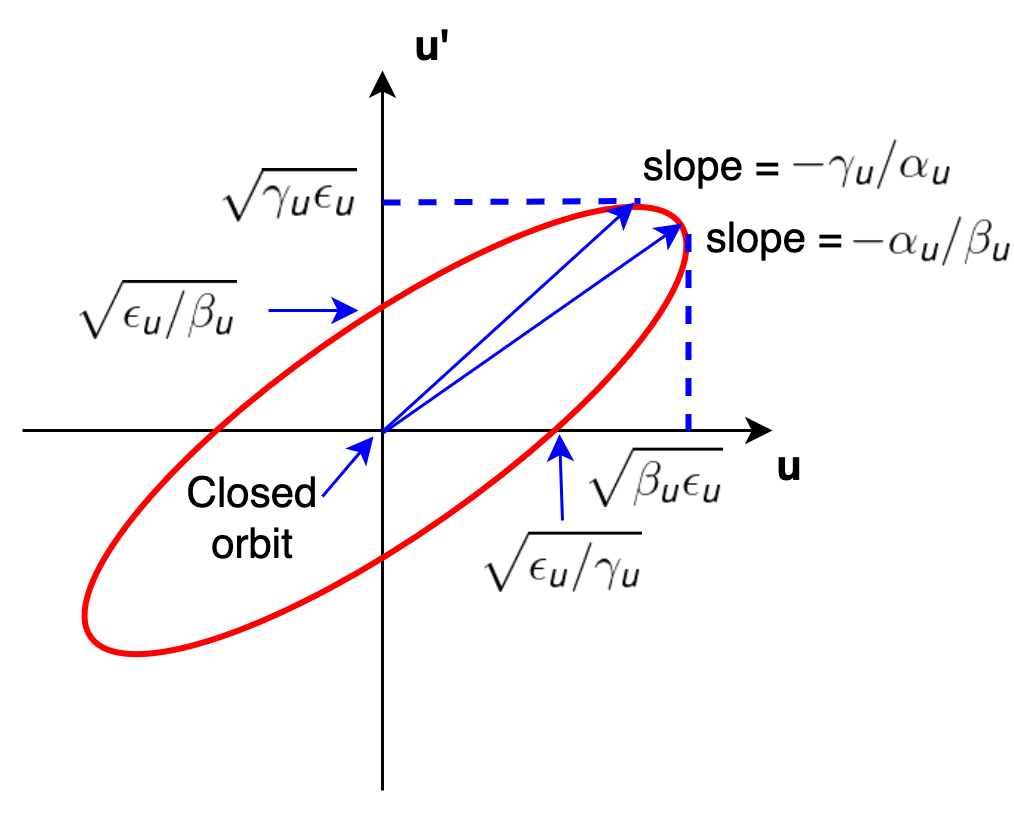
\includegraphics[width=0.6\textwidth]{images/Ch2/phase_space_ellipse.png}
        \caption{Phase space co-ordinates $(u, u^\prime)$ turn by turn, for a particle moving along the ring but at a particular position $s$ which is characterised by the following twiss parameters $[\alpha_u(s), \beta_u(s), \gamma_u(s)]$. For the plotting, the dependence on the $s$ parameter has been omitted.}
        \label{fig:phase_space_ellipse}
 \end{figure}

\textbf{Transvserse emittance}\\
Up to now, the twiss parameters were used to describe the dynamics of single particles. However, they also describe the distribution of the particles within a bunch. The statistical average of $u^2$ over all particles at a given point $s$ along the reference trajectory, from Eq.~\eqref{eq:position_action_anlge} equals to~\cite{wolski2014}:
\begin{equation}\label{eq:statistical_average_position}
    \langle u^2(s) \rangle = 2 \beta_u(s) \langle J_u \cos^2{\psi_u(s)} \rangle.
\end{equation}
Assuming, that the angle and action variables are uncorrelated and that the angle variables are uniformly distributed: % angles uniformly distributed from (0,2pi)
\begin{equation}\label{eq:mean_u_zerp}
    \langle u(s) \rangle = 0,
\end{equation}
and then Eq.~\eqref{eq:statistical_average_position} becomes:
\begin{equation}\label{eq:emittance_definition_1}
    \langle u^2(s) \rangle = \beta_u(s) \epsilon_u,
\end{equation}
where
\begin{equation}\label{eq:geom_emittance_action}
    \epsilon_u=\langle J_u \rangle
\end{equation}
is the geometric emittance of the bunch. Considering the same assumption Eq.~\eqref{eq:position_action_anlge} and  Eq.~\eqref{eq:divergence_action_anlge} results to:
\begin{equation}\label{eq:u_uprime_eq_1}
    \langle u(s) u^\prime(s) \rangle = - \alpha_u(s) \epsilon^{\mathrm{geom}}_u,
\end{equation}
\begin{equation}\label{eq:u_uprime_eq_2}
    \langle u^{\prime 2}(s) \rangle = \gamma_u(s) \epsilon^{\mathrm{geom}}_u.
\end{equation}

Combining the above equations, the geometric emittance is expressed in terms of the particles' distribution as:

\begin{equation}\label{eq:geometric_emittance_v2}
    \epsilon^{\mathrm{geom}}_u = \sqrt{\langle u^2(s) \rangle \langle u^{\prime 2}(s) \rangle- \langle u (s)u^{\prime}(s) \rangle ^2}
\end{equation}

which, for $\langle u(s) \rangle=0$ (Eq.~\eqref{eq:mean_u_zerp}), equals the covariance or Sigma matrix of the particles' distribution (Eq~\eqref{eq:Sigma_matrix}):

\begin{equation}\label{eq:Sigma_matrix}
    \Sigma = \begin{pmatrix}
        \langle u^2(s) \rangle & \langle u(s) u^\prime(s) \rangle \\ 
        \langle u(s) u^\prime(s) \rangle & \langle u^{\prime 2}(s) \rangle 
        \end{pmatrix}  = \begin{pmatrix}
            \sigma_u^2(s) & \langle u(s) u^\prime(s) \rangle \\ 
            \langle u(s) u^\prime(s) \rangle & \sigma_{u^{\prime 2}(s)} 
            \end{pmatrix} 
\end{equation}

The square root of the top-left element of the Sigma matrix, $\sigma_u$, is defined as the rms beam size and is also a variable that is used extensively in accelerator physics. The definition of rms and of others of the statistical analysis can be found in Appendix~\ref{ch:app_A}.

Figure~\ref{fig:phase_space_emittance} provides a visualisation of the concepts of emittance and rms beam size. It shows the phase space of a transverse Gaussian bunch along with the histograms of the $u$ (top) and $u^\prime$ (right) variables at a particular point $s$ along the ring. Each particle follows its individual ellipse (of different sizes but with the same orientation) depending on its initial conditions. The rms beam size, $\sigma_u$, and the rms normalised momentum spread, $\sigma_{u^\prime}$, are shown in the top and right histograms of Fig.\ref{fig:phase_space_emittance} with the blue vertical lines. This corresponds to the area of the ellipse enclosed in the blue line in the phase space plot and equals the rms or geometric emittance, $\epsilon^{\mathrm{geom}}_u$ , as defined in Eq.~\eqref{eq:geometric_emittance_v2}.

\begin{figure}[!h] 
    \centering         
    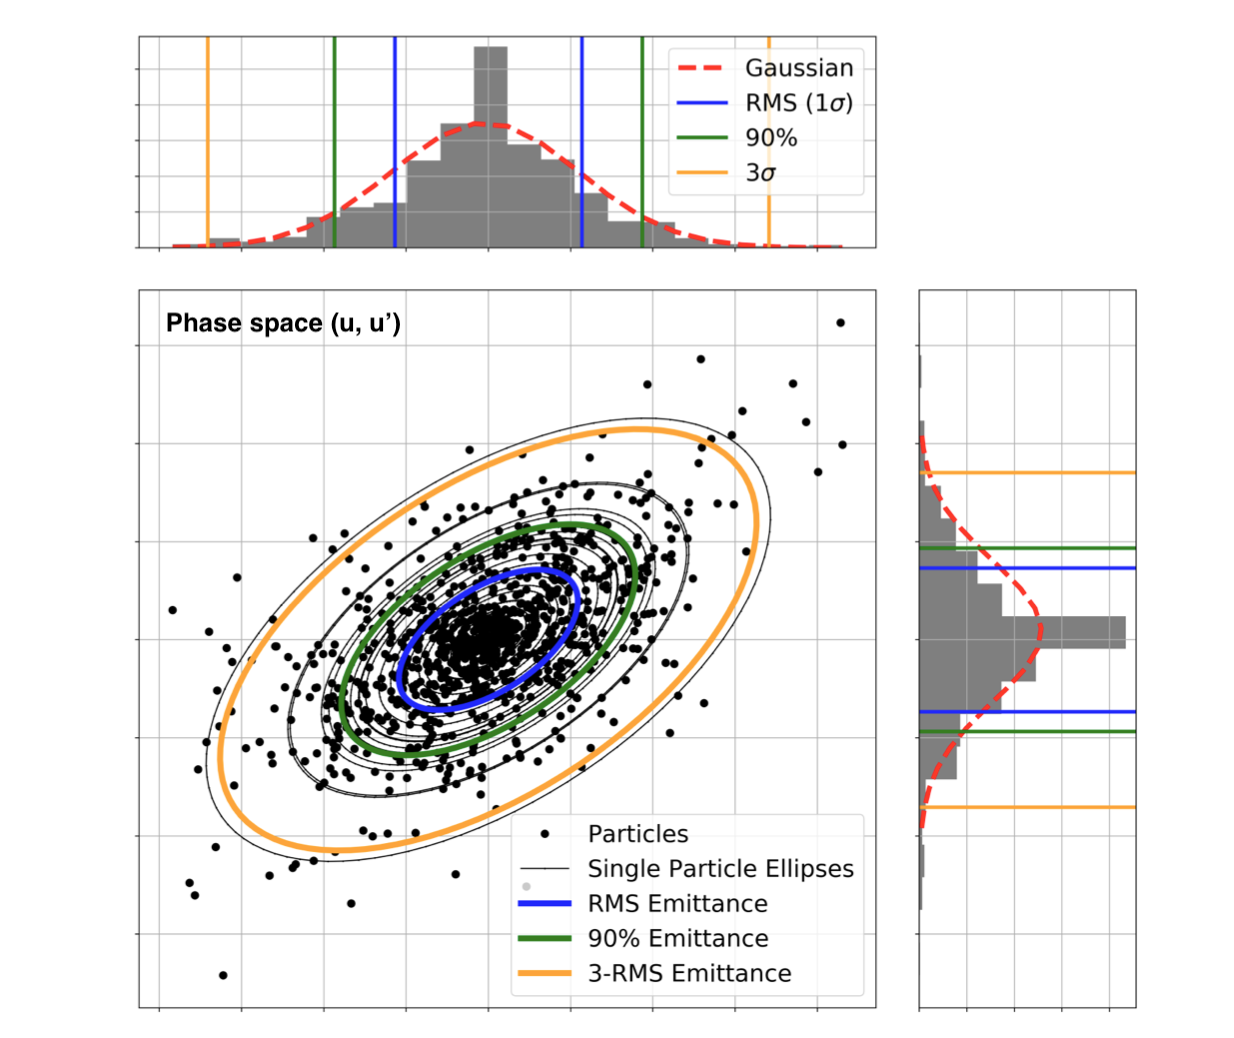
\includegraphics[width=0.9\textwidth]{images/Ch2/transverse_phase_space_emittance.png}
        \caption{Transverse phase space of a Gaussian bunch. The figure is a courtesy of Tirsi Prebibaj~\cite{tirsi_thesis_presentation}.}
        \label{fig:phase_space_emittance}
 \end{figure}

It should be noted, that there are also other conventions to define the emittance such as the 90$\%$ emittance (green lines in Fig.~\ref{fig:phase_space_emittance}) or the 3-sigma emittance (yellow lines in Fig.~\ref{fig:phase_space_emittance}). However, here the term geometric emittance will refer to the rms geometric emittance.

According to Liouville’s theorem~\cite{wolski2014}, considering that there are no interactions between the particles and that the energy of the beam is not changing, the geometric emittance remains constant and therefore is an invariant of bunch motion (similarly to the action $J_u$ for the single-particle motion). The geometric emittance does not remain constant during acceleration, instead the normalised emittance is defined as:
\begin{equation}\label{eq:normalised_emittance}
    \epsilon_u = \beta_0 \gamma_0 \epsilon^{\mathrm{geom}}_u
\end{equation}
The normalised emittance is conserved during acceleration and therefore it is most often used in accelerator physics. It is highlighted here, that throughout this thesis the term "emittance" will refer to the rms normalised emittance.

It is worth commenting here, that for the simulation studies presented in this thesis, the emittance is computed using the statistical definition introduced in Eq.~\eqref{eq:geometric_emittance_v2}. In the experimental studies, the emittance is obtained with a Gaussian fit of the bunch distribution, to obtain its $\sigma$. This process is explained extensively in Chapter~\ref{Ch:2018_analyisis}. For that case, the normalised emittance is obtained from the following formula which is obtained form Eq.~\eqref{eq:emittance_definition_1}, Eq.~\eqref{eq:Sigma_matrix} and Eq.~\eqref{eq:emit_geom_norm_relation}:

% For a Gaussian beam distribution the normalised beam emittance it applies:
\begin{equation}\label{eq:emit_from_beam_size}
    \epsilon_{u} = \frac{\sigma_u(s)^2}{\beta_u(s)} \beta_0 \gamma_0,
\end{equation}

where $\sigma_u(s)$ is the rms beam size, $\beta_u(s)$ is the beta function, at specific location $s$ along the accelerator and $\beta_0, \gamma_0$ are the relativistic parameters. 

It should be highlighted that the emittance definitions of Eq.~\eqref{eq:geometric_emittance_v2} (after normalisation with the relativistic parameters) and of Eq.~\eqref{eq:emit_from_beam_size} are equivalent.

Finally, despite Liouville’s theorem in a real accelerator there are various phenomena that change the emittance such as~\cite{Buon:216507}: scattering on residual gas, intra-beam scattering, beam-beam scattering, stochastic or electron cooling, synchrotron radiation emission, filamentation due to non-linearities of the machine, space charge and noise effects. The studies in this thesis focus on the emittance growth due to noise effects (discussed in more details in Chapter~\ref{Ch:CC_noise_theory}).

\textbf{Normalised phase space}\\
Often in accelerator physics it is useful to transform the transverse phase space ellipse to a normalised phase space circle, where the co-ordinates are normalised with the twiss parameters for the particular location $s$ around the ring.

normalised emittance of the initial beam distribution, $\epsilon_{u,0}$.



 Federicos thesis 2.3.1 and sondre eq. 2.21a


\textbf{Off-momentum effects - dispersion}\\
Up to now, the discussion was limited to on-momentum particles $\delta=0$: their momentum equals the reference momentum, $p_0$. In a more realistic beam, however, the momentums of the individual particles are spread around the reference one $p_0$ and this is expressed with the longitudinal co-ordinate $\delta=(p-p_0)/p_0$ defined in Eq.~\eqref{eq:particle_coordinates}. As an example, in the SPS machine, which is of interest for this thesis, $\delta$ is in the order of magnitude of $10^{-4}$ to $10^{-3}$.

The off-momentum particles experience different forces than the reference particle when passing through the magnetic fields in an accelerator. Here their motion through the dipole magnets which leads to dispersion effects is discussed. 

Particles with $\delta < 0$ ($\delta>0$) are deflected stronger (less) by the dipole magnets than the reference particle due to lower (higher) magnetic rigidity. Therefore, they travel along the accelerator performing betatron oscillations not around the reference trajectory but around a different closed orbit as illustrated in Fig.~\ref{fig:closed_orbit_Dx} which depends on their momentum spread $\delta$. This dependence of the closed orbit on the momentum offset of the particle is called dispersion.

\begin{figure}[!h] % 
    \centering         
    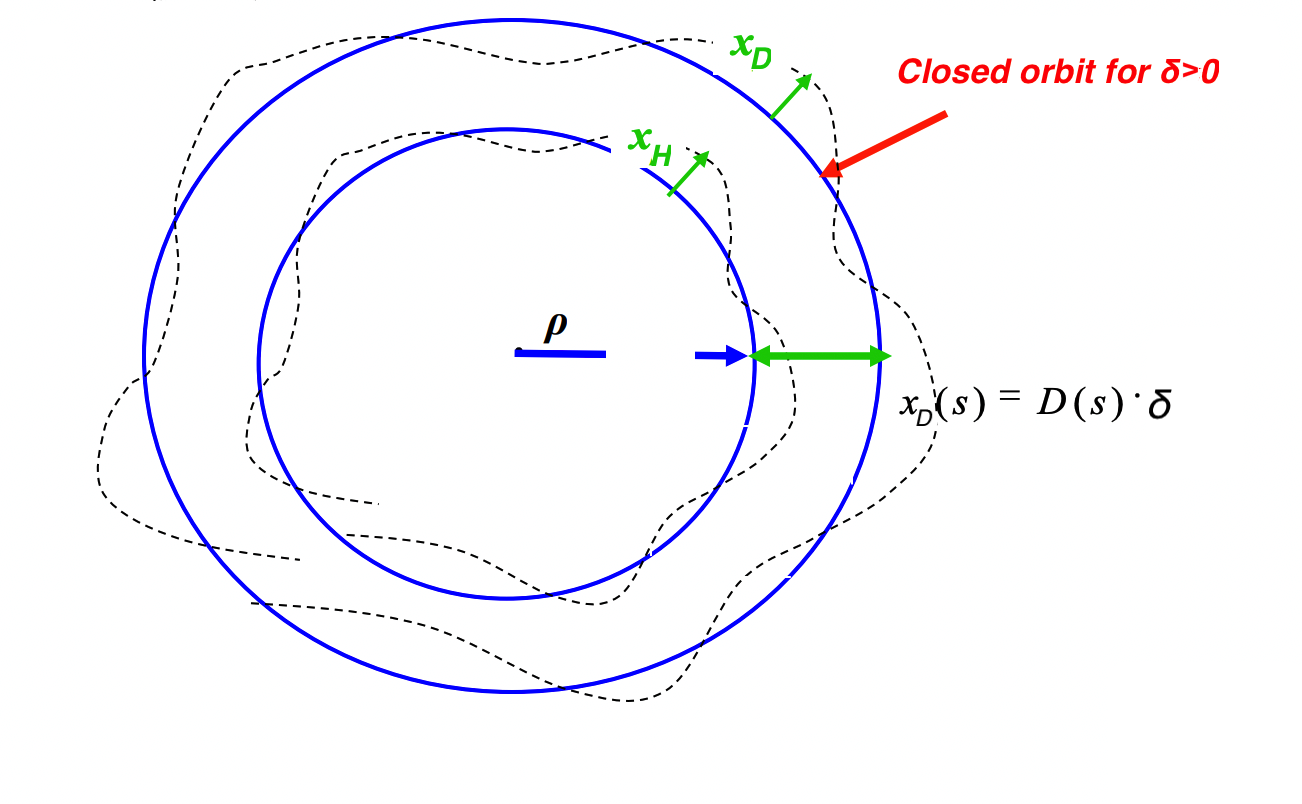
\includegraphics[width=0.6\textwidth]{images/Ch2/closed_orbit_dispersion.png}
        \caption{The closed orbit and the betatron oscillations around it in the presence of dispersion~\cite{Holzer_summer_students_introduction}}
        \label{fig:closed_orbit_Dx}
 \end{figure}

The equation of motion for the off-momentum particles is:
\begin{equation}
    x^{\prime \prime}(s) + K_x(s)x(s) = \frac{1}{\rho(s)} \delta,
\end{equation}
with the following solution:
\begin{equation}
    x(s) = x_H(s) + D_x(s)\delta,
\end{equation}
where $x_H(s)$ is the homogeneous solution shown in Eq.~\eqref{eq:position_action_anlge} and $D_x(s)$ is the dispersion function which can be expressed as:
\begin{equation}\label{eq:dispersion_function}
    D^{\prime \prime}_x(s) + K_x(s)D_x(s) = \frac{1}{\rho(s)}.
\end{equation}

%Its solution is the sum of the solutions of homogeneous (for $\delta=0$) and of the inhomogeneous ($\delta \neq 0$) equation:
%\begin{equation}
%    x(s) = x_H(s) + x_I(s) = x_H(s) + D_x(s)\delta,
%\end{equation}

% which is defined as:
%\begin{equation}\label{eq:dispersion_function}
%   D_x(s) = \frac{x_I(s)}{\delta}
%\end{equation}

The dispersive contribution can be added to the transfer matrix introduced in Eq.~\eqref{eq:matrix_formalism_intro} as follows:
\begin{equation}\label{eq:matrix_formalism_dispersion}
    \begin{pmatrix}
     x\\ 
     x^\prime
     \end{pmatrix}_{s_1} = M_x (s_1 |  s_0) \begin{pmatrix}
     x\\ 
     x^\prime
     \end{pmatrix}_{s_0} + \delta \begin{pmatrix}
        D_x\\ 
        D_x^\prime
        \end{pmatrix}_{s_0}.
 \end{equation}
%The transfer matrix $M$ can be re-written such as it inclyyded, alide 14 in presentation v2 below:

% 1. Definition of D: https://yannis.web.cern.ch/teaching/transverse.pdf
% 2. Definition of D prime: https://indico.cern.ch/event/847209/contributions/3558973/attachments/1932901/3201996/AccPhys_Lect7_MomEff.pdf

 From the discussion above, it becomes clear that the dispersion couples the longitudinal with the horizontal motion. The dispersion effects are discussed here only for the horizontal plane due to the fact that (as stated already) only vertical dipolar fields are considered. As an example, the rms vertical dispersion of the SPS machine is about 1.8\,m (model value). %/Users/nataliatriantafyllou/PhD_projects/exploring_SPS/madx_studies/optics_new_seq_after_LS2/output/twiss_thin_elements
 
 At this point, it is appropriate to mention that only the model vertical dispersion equals zero. In a real machine, vertical dispersion can be introduced by sources such as the steering errors of the dipole or quadrupole magnets~\cite{Wolski_uspas}. As an example, the rms vertical dispersion in the SPS machine is measured to be about 10\,cm.

Finally, in the presence of dispersion the normalised beam emittance (Eq.~\eqref{eq:emit_from_beam_size}) becomes:
\begin{equation}\label{eq:emit_from_beam_size_Du}
    \epsilon_{u} = \frac{\sigma_u(s)^2 - \delta^2 D_u^2(s)}{\beta_u(s)} \beta_0 \gamma_0,
\end{equation}
where $\sigma_u(s)$ is the rms beam size, $\beta_u(s)$ is the beta function, $D_u(s)$ is the dispersion fat a specific location s along the accelerator, $\delta$ is the momentum spread and $\beta_0, \gamma_0$ the relativistic parameters.

Additionally, the off-momentum particles receive different focusing due to gradient errors in the quadrupoles. This effect is known as chromaticity and is discussed in detail in the next subsubsection which focuses on non-linear beam dynamics.

\subsubsection{Non-linear dynamics}
Up to now, only linear elements (dipoles and quadrupoles) were considered as in theory they are sufficient to create a synchrotron. However, in a real machine non-linearities are also present due to factors such as imperfections in the magnets field and alignment, particles' momentum spread, and higher order magnets (sextupoles, octupoles, etc). Here, the preceding discussion is expanded to include the non-linear beam dynamics. The discussion is limited in the two effects that are important for the work presented in this thesis: the chromaticity and the detuning with transverse amplitude.

\textbf{Chromaticity}\\
We define the chromaticity as the variation of the betatron tune $Q_u$ with the relative momentume deviation delta. This is a result of the fact that particles with $\delta < 0$ ($\delta > 0$) recieve a weaker (stronger) focusing strength from the quadrupoles due to their larger magnetic rigidity. The tune shift introduced by the chromaticity for each particle, $ \Delta Q_u (\delta)= Q_u - Q_{u0}$, is: % M. Schenk p.49

%The tune shift introduced by the chromaticity is: % M. Schenk p.49

\begin{equation}\label{eq:chromatic_tune_shift_up_to_order_m}
   \Delta Q_u (\delta) = \sum_{n=1}^m \frac{1}{n!} Q_u^{n} \delta^n, 
\end{equation}
where:
\begin{equation}\label{eq:chroma_up_to_order_m}
    Q_u^{n} = \left. \frac{\partial ^n Q_u}{\partial \delta^n} \right|_{\delta=0}, n \in \mathbb{N},
 \end{equation}
denotes the chromaticity of order $n$. The studies in this thesis, are limited to the chromaticity at the first order in $\delta$ $(n=1)$ which is often called linear chromaticity. 

Large values of chromaticity can lead to instabilites and therefore to beam loss. Sextupole magnets are typically used to control the natural chromaticity of a machine and achieve the desired values for its operation.

The chromaticity like the tune is a property of the machine lattice. % the chromaticity is one number

\textbf{Octupoles and detuning with amplitude}\\
Octupole magnets are most often used to increase the transverse tune spread of the beam particles to avoid resonances \footnote{Resonances in circular accelerators are a result of perturbation terms in the equation of motion once the perturbation frequency matches the frequency of the particles' oscillatory motion. The topic of resonances is out of the scope of this thesis, however, more details can be found in Chapter 16 of Ref.~\cite{Wiedemann:1083415}} and instability effects  \footnote{Beam instabilities in an accelerator are a result of the interplay of the wakefields (will be discussed in Section~\ref{subsec:wakefields}) and a perturbation (e.g. noise) on equations of motion of the beam particles. Similar to the resonances their detailed study is out of the scope for this thesis, however more details can be found in Ref.~\cite{Rumolo:1982422}.}.

In the SPS and LHC rings, the octupoles are installed in families (focusing and defocusing) in order to avoid the excitation of resonances and they are called "Landau octupoles" as they are used to create a betatron tune spread that provides the mechanism of Landau damping~\cite{Herr:1982428} (to stabilise the beam).

The betatron tune spread that is introduced by the octupoles is action-dependent in both transverse planes. In terms of the normalised actions (sondre)

\subsection{Longitudinal motion}
In the longitudinal plane the motion is tangential to the reference trajectory and is described by the co-ordinates $(z, \delta)$. 



\section{Collective effects}
\subsection{Impedance and wakefields}\label{subsec:wakefields}

\subsection{Active feedback?}
\section{Optics models of accelerators}
% or optics design
\subsection*{MADX}
Table with parameters for sps lattice, eg average beta function, tune etc. circumference, Q20 and Q26.

presentation AUTH?


See sondre's thesis for inspiration on the structure.
\section{General parameters of the studies}
% Maybe this should be mentioned at the end of project objectives and thesis outline.
% The following paragraphs are taken from the APR Ch.1.3 
\subsection{SPS optics}\label{subsec:SPS_optics_model}
 The studies presented in this thesis were performed for the nominal SPS optics for the LHC filling which are called Q26 optics as the higher integer part of the tune in both planes is 26. 

 \normalsize{\textbf{SPS nominal model}\\
 The model for the Q26 optics can be found in the official CERN repository~\cite{SPS_optics_repo} and will be referred to as the nominal SPS model in this thesis. The values of the optics parameters in what follows correspond to the model values unless stated otherwise.

 \normalsize{\textbf{SPS non-linear model}\\
\textcolor{red}{Move this section to chapter 6.}
The nominal SPS model includes only the nonlinear fields produced by the chromatic sextupoles. However, one of the most important sources of non-linearities in SPS are the odd multipole components of its main dipole magnets. For some of the studies presented in this thesis their impact on the beam dynamics must be studied and therefore they should be included in the nominal model. 

% APR Chapter 3.1
The multipole error of the SPS main dipoles are unfortunately not available from magnetic measurements. On this ground a non-linear optics model of the SPS has been established with beam-based measurements of the chromatic detuning over a range of momentum deviation~\cite{Carlà:2664976, Alekou:2640326}.  The optics model was obtained by assigning systematic multipole components to the main lattice magnets, in the nominal model of SPS, in order to reproduce the tune variation with themomentum deviation as it was measured in the real machine. The calculations were performed with MAD-X [].

The values of the multipole components up to seventh order obtained from this method are given in Table~\ref{tab:sps_mult_270GeV} where, ($b_3^A, b_3^B$) ($b_5^A, b_5^B$) and ($b_7^A, b_7^B$) stand for the sextupolar, decapolar and decatetrapolar mutipoles respectively. Note that different values have been obtained foreach of the two different kinds of SPS main dipoles (MBA and MBB) which are marked withthe indices A and B respectively.

\begin{table}[ht] % table take from the APR
    \caption{Multipole errors from SPS non-linear model, at 270\,GeV.} % title of Table
    \centering % used for centering table
    \begin{tabular}{c c c c} % centered columns (4 columns)
    \hline\hline %inserts double horizontal lines
    Multipole & Value  \\ [0.5ex] % inserts table
    %heading
    \hline  % inserts single horizontal line
    $b_3^A, b_3^B$ & 8.1 $\times 10^{-4}$\,$\mathrm{m^{-2}}$, 1.1 $\times 10^{-3}$\,$\mathrm{m^{-2}}$\\ 
    $b_5^A, b_5^B$ & 9.2\,$\mathrm{m^{-4}}$, $-$10\,$\mathrm{m^{-4}}$ \\
    $b_7^A, b_7^B$ & 1.3 $\times 10^{5}$\,$\mathrm{m^{-6}}$, 1.4 $\times 10^{5}$\,$\mathrm{m^{-6}}$\\ [1ex] % [1ex] adds vertical space
    \hline %inserts single line
    \end{tabular}
    \label{tab:sps_mult_270GeV} % is used to refer this table in the text
    \end{table}


\textbf{random multiple errros? } Like in APR.Ch.3.2.2.

\section{Transfer maps}
Need to mention them briefly as you refer to them at the PyHEADTAIL section.

% Courant snyder formalism of longitudinal dynamics: https://journals.aps.org/prab/pdf/10.1103/PhysRevAccelBeams.24.094001
\section{Action angle variables}
The action for the x-plane is:

\begin{equation}\label{eq:action}
    \Jx = \frac{1}{2}(x_n^2 +xp^2_n) 
\end{equation}
where 
\begin{equation}\label{normalised_y}
    x_n = \frac{x}{\sqrt{\beta_x}}, \ \ xp_n = \frac{\alpha_x x}{\sqrt{\beta_x}} + \sqrt{\beta_x}xp
\end{equation}
the normalised coordinates and $\alpha_y, \beta_y$ the twiss parameters. 
The same applies for the y-plane. 

s
The statistical geometric emittance equals the average of the actions distribution:
\begin{equation}\label{eq:geom_emit_actions}
    \emitxgeom = \langle \Jx \rangle
\end{equation}
%\begin{equation}\label{eq:geom_emit_actions}
%    \epsilon_x^{\mathrm{geom}} = \langle \Jx \rangle
%\end{equation}
The distribution of actions is an exponential distribution (further explanation needed?). Therefore, its mean equals its standard deviation. (this property is used in the appendix for the computation of the rms tune spread.)

From Eq.~\eqref{eq:action} we write:
\begin{equation}\label{eq:Jy_exp_distr}
    e^{-J/\epsilon} = e^{(-x^2/2\epsilon - px^2/2\epsilon)}
\end{equation}
From this equation it can be seen that the actions follow an exponential distribution. 

\section{Wakefields and impedances}\label{sec:wakefields_theory}

he terms dipolar and quadrupolar have been chosen as the dipolar wake function acts on the test proton like a dipole magnet (the kick is the same whatever its transverse location), whereas the quadrupolar term acts like a quadrupole magnet (the kick increases linearly with the transverse offset of the test particle). Benoits thesis p.44


\section{Tracking simulation codes}\label{sec:simualtion_codes}
In this section the two tracking simulation codes used in this thesis to study the noise-induced emittance growth are presented. Both codes are macroparticle tracking libraries that simulate the particle motion in the six-dimensional (6D) phase space $(x, x^\prime, y, y^\prime, z, \delta)$. The first code performs tracking between interaction points around a circular accelerator with the use of trasnfer matrices while the second one uses the detailed optics model of the machine.

\subsection{PyHEADTAIL}\label{subsec:pyheadtail}

PyHEADTAIL~\cite{pyheadtail_repository} is an open-source 6D macroparticle tracking code, developed at CERN, which was originally designed to study collective effects in circular machines and to be easily extrensible with custom elements. 
% https://indico.cern.ch/event/930271/contributions/3910265/attachments/2066139/3467770/30June2020_Simulations_emit_growthCC_RFnoise.pdf  
Details on its implementation and its features can be find in Refs.~\cite{pyheadtail_manual_adrian, pyheadtail_schenk}. Below the main steps of a simulation are listed: % according to the interest of this thesis.

% Thesis david: https://cds.cern.ch/record/2707064/files/CERN-THESIS-2019-272.pdf (p.45) and for the transverse matrix.

\begin{enumerate}
    \item \textbf{Machine initialisation:} The accelerator ring is splitted into a number of segments of equal length, after each of which there is an interaction point (IP). At the interaction points the macroparticles experience kicks from various accelerator components (feedback system, multipoles etc) or from collective effects such as the wakefields. The machine parameters, such as the circumference, the betatron and synchrotron tunes and the optics at the interaction points are defined. It should be noted that PyHEADTAIL uses smooth approximation which means that only a few segments are defined per turn. % which results to a very  rough optics model.
    \item \textbf{Bunch initialisation:}  A particle bunch is represented by a collection of macroparticles, each of which represents a clustered collection of physical particles. Each macroparticle is described by four transverse $(x, x^\prime, y, y^\prime)$ and two longitudinal coordinates $(z, \delta)$, a mass and an electric charge. For the studies presented in this thesis $10^{5}$ macroparticles are sufficient for an accurate represantation of the bunch, unless it is stated otherwise. There are various distributions available. In this thesis the simulations are performed using a Gaussian distribution in transverse and longitudinal planes.
    \item \textbf{Transverse tracking}: In the transverse plane, the macroparticles are transported from one interaction point to another by linear transfer matrices which take into account the optics parameters at the beginning and the end of the corresponding segment. For example, in the horizontal plane the transport of each macroparticle from IP1 to IP2 along the ring is given by:
    \begin{equation}
        \binom{x_i}{x_i^\prime}_{\mathrm{IP0}} = M \binom{x_i}{x_i^\prime}_{\mathrm{IP1}},
    \end{equation}
    where $i=1, ..., N$ with N being the number of macroparticles and the matrix $M$ is given by:
    \begin{equation}\label{eq:linear_transfer_map}
        M = \begin{pmatrix}
            \sqrt{\beta_{x, \mathrm{IP0}}} & 0 \\ 
            -\frac{\alpha_{x, \mathrm{IP0}}}{\sqrt{\beta_{x,  \mathrm{IP0} }}} & \frac{1}{\sqrt{\beta_{x, \mathrm{IP0}}}}
            \end{pmatrix} \begin{pmatrix}
                \cos(\Delta \mu_{x, \mathrm{IP0 \to IP1 }}) & \sin(\Delta \mu_{x, \mathrm{IP0 \to IP1 }})\\
                 - \sin(\Delta \mu_{x, \mathrm{IP0 \to IP1 }})  &\cos(\Delta \mu_{x, \mathrm{IP0 \to IP1 } }) 
                \end{pmatrix}  \begin{pmatrix}
                    \sqrt{\beta_{x, IP1}} & 0 \\ 
                    -\frac{\alpha_{x, IP1}}{\sqrt{\beta_{x, IP1}}} & \frac{1}{\sqrt{\beta_{x, IP1}}}
                    \end{pmatrix} 
    \end{equation}
    where $\alpha_{x, \mathrm{IP0/IP1}}$ and $\beta{x, \mathrm{IP0/IP1}}$ are the optics paramters at the interaction points IP0 and IP1 respectively and $\Delta \mu_{x, \mathrm{IP0 \to IP1 }}$ the phase advance from IP0 to IP1. As smooth approximation is used, the phase advance equals: 
    \begin{equation}\label{eq:phase_advance_smooth_approximation}
        \Delta \mu_{x, \mathrm{IP0 \to IP1 }} = Q_x \frac{L}{C},
    \end{equation}
    where $Q_x$ is the horizontal betatron tune, $C$ the machine circumference and $L$ the length of the corresponding segment. It should be noted that if no detuning source is added (see next step) the matrix $M$ is the same for all particles.
    \item \textbf{Chromaticity and detuning with transverse amplitude:} The chromaticity (up to higher orders) and amplitude detuning are implemented as a change of the phase advance of each individual particle as follows (example for the horizontal plane):
    \begin{equation}\label{eq:change_phase_advance_detunign}
        \Delta \mu_{x, i \mathrm{IP0 \to IP1 }} = \Delta \mu_{x, \mathrm{IP0 \to IP1 }} + (\xi^{1}_x \delta_i + \alpha_{xx}J_{x, i} + \alpha_{xy}J_{y,i}) \frac{\Delta \mu_{x, \mathrm{IP0 \to IP1 }}}{2\pi Q_x}, 
    \end{equation}
    where $i=1, ..., N$ with N being the number of macroparticles, $\Delta \mu_{x, \mathrm{IP0 \to IP1 }}$ is the phase advance for all macroparticles defined in the previous step, $\xi_x^{1}$ the horizontal chromaticity of first order normalised to the tune $\alpha_{xx}$ and $\alpha_{xy}$ are the detuning coefficients, while $J_x$ and $J_y$ are the horizontal and vertical actions of the macroparticle. Therefore, in the presence of detuning the elements of the $M$ matrix are different for every particle.

    \item \textbf{Longitudinal tracking:}  In PyHEADTAIL the longitudinal particle dynamics are described with the longitudinal equations of motion (ref to eq earlier.) % slide 37: https://www2.kek.jp/accl/legacy/seminar/file/PyHEADTAIL_PyECLOUD_2.pdf 
    The longitudinal coordinates are advanced once per turn after solving numerically the equations of motion~\cite{pyheadtail_schenk}. The motion can be linear or not (non-linear RF system). The studies presented in this thesis use the linear longitudinal tracking.

    \item \textbf{Trasnverse impedance effects:} In PyHEADTAIL, wakefield kicks are used to implement the effect of the transverse impedance in time domain. To improve the computational efficiency, the total impedance of the full machine is lumped in one of the interaction points along the ring and the kicks are applied on the macroparticles once per turn. Additionally, instead of computing the wakefield kicks from each particle to the rest individually, the bunch is divided in a number of longitudinal slices and the macroparticles in each slice recieve a wakefield kick generated by the preceding slices\footnote{This is valid in the ultrarelativistic scenario when no wakefield is generated in front of the bunch. The condition applies for the SPS experiments described in this thesis, performed at 270\,GeV.}~\cite{Salvant:1274254}. This is illustrated schematically in Fig.~\ref{fig:longitudinal_slicing_wakefields}. A large number of slices is required such as the wakes can be assuemed constant within the slice. A high number of macroparticles is also needed in order to avoid statistical noise effects caused by undersampling~\cite{pyheadtail_manual_adrian}. For the studies presented in 500 slices are used over a range of three rms bunch lengths in both directions from the bunch center with the bunch being represented by $10^6$ macroparticles (instead of $10^5$ required for simulations without impedance effects).
    

    \begin{figure}[!ht]
        \centering
        \begin{subfigure}[t]{0.45\textwidth}
            \centering
            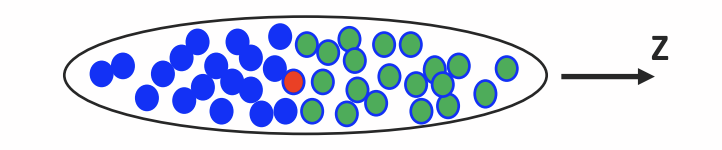
\includegraphics[width=1\textwidth]{images/Ch2/before_slicing.png}
            \caption{Without slicing}
            %\label{fig:add_label_here}
        \end{subfigure}
        \hfill
        \begin{subfigure}[t]{0.45\textwidth}
            \centering
            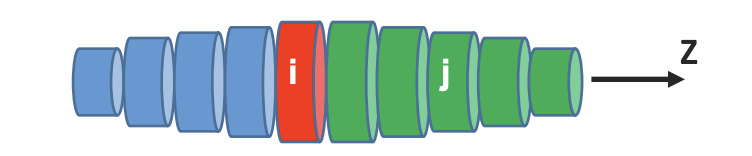
\includegraphics[width=1\textwidth]{images/Ch2/after_slicing.png}
            \caption{With slicing}
            %\label{fig:add_label_here}
        \end{subfigure}
        \hfill
         \caption{Longitudinal bunch slicing for the implementation of wakefields kicks in PyHEADTAIL. Without the slicing technique (left) the wake kicks on the red macroparticle are generated from all the green macroparticles resulting to computationally heavy simulations. Instead, when the bunch is sliced longitudinally (right) the wake kicks on the macroparticles in the red slice $i$ are generated by the macroparticles in the green slices $j$, decreasing significantly the computation time. The figures are a courtesy of M. Schenk~\cite{pyheadtail_schenk}} % bunch passage
         \label{fig:longitudinal_slicing_wakefields}
     \end{figure}
        
    The wakefield kicks are computed using a convolution of the wake function with the moments of each particle. %p.39 michael schenk thesis
    The wake functions are available from detailed imepdance model of the machine which are obtained from a combination of theoretical computations, electromagentic simulations and can be imported in PyHEADTAIL in form of tables. More details on the SPS impedance model are provided in Section~\ref{sec:sps_impedance_model}.
    
    \item \textbf{Data acquisition:} The updated bunch coordinates after each turn are available at IP0 for post processing. Typically, $10^{5}$ turns are required for the noise-induced emittance growth simulation presented in this thesis. 
    
\end{enumerate}


%Last sentence from (LinearMap): https://github.com/PyCOMPLETE/PyHEADTAIL/blob/master/PyHEADTAIL/trackers/longitudinal_tracking.py
%or longutidanl equations of motion: slide 37 https://www2.kek.jp/accl/legacy/seminar/file/PyHEADTAIL_PyECLOUD_2.pdf

Figure~\ref{fig:pyheadtail_accelerator_model} shows a graphic representation of the accelerator model and the tracking procedure supporting the steps described above.
% Graph is created app.diagrams.net and is saved in goodle dirve.

\begin{figure}[!h]
    \centering         
    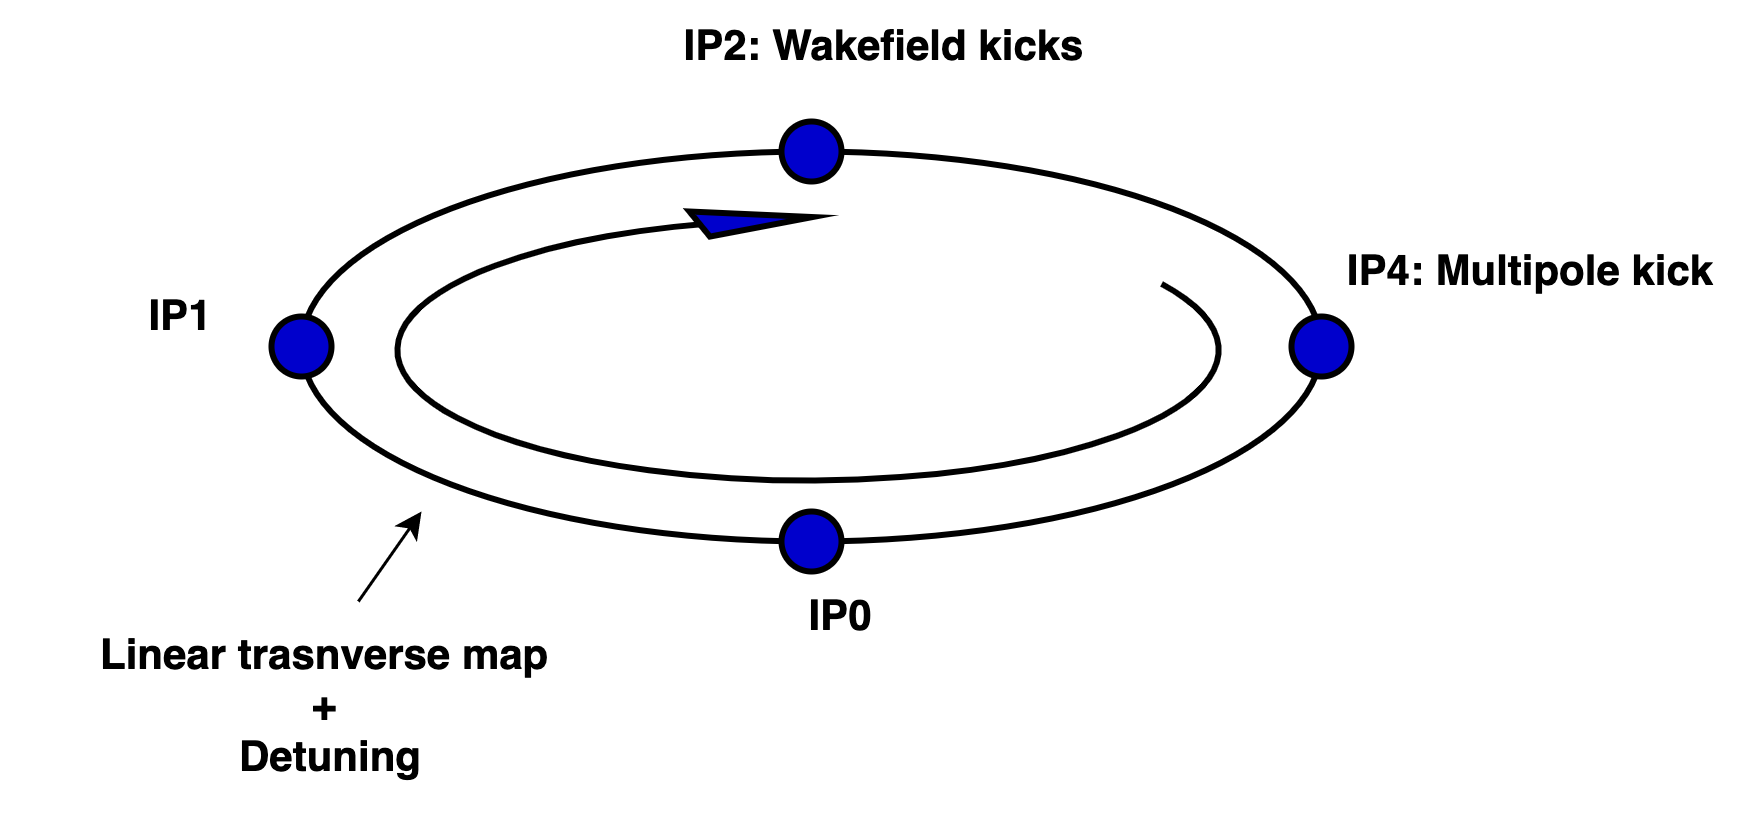
\includegraphics[width=0.6\textwidth]{images/Ch2/accelerator_model_graph_pyheadtail.png}
        \caption{Graphic represantation of the accelerator model and tracking procedure in PyHEADTAIL (inspered by the graphs in Refs.~\cite{pyheadtail_schenk, inproceedings_ibs_pyheadtail}). In this example the ring is splitted in four segments seperated by the interaction points (IPs). Wakefield and mulitple kicks are applied on the macroparticles in IP2 and IP4. The macroparticles are transported between the IPs by a linear map (which can include detuning effects) in the transverse plane.  The longitudinal coordinates are updated once per turn without being visualised in this plot.}
        \label{fig:pyheadtail_accelerator_model}
 \end{figure}


\subsection{Sixtracklib}\label{subsec:sixtracklib}
%Introduction to sixtrackib: https://indico.cern.ch/event/833895/contributions/3577803/attachments/1927226/3190636/intro_sixtracklib.pdf
% https://inspirehep.net/files/6273430c727ace3796a92d069f651ade


Check a presentation from kostas.

\chapter{Theory of Crab Cavity noise induced emittance growth}\label{Ch:CC_noise_theory}
This section describes the theoretical formalism which predicts the transverse emittance growth in the presence of $\CC$ RF noise. First, it introduces the concept of noise in accelerator physics. The second section focuses on the $\CC$ amplitude and phase noise and it provides the equations to predict the noise-induced emittance growth. The last section comments briefly on the experiments that were carried out in KEKB: the work at KEKB constitutes the only experimental study of the effect of crab cavity RF noise prior to the work performed in the SPS 



%You need the frist section to introduce the dipole noise as you will apply it in the simulations.
\section{Noise}\label{sec:noise_definition}
%External noise means that it is independent of the beam itself.
In particle accelerators, the presence of noise in components controlling the beam or observing the beam behaviour is a concern. Random fluctuations in the electric and magnetic fields seen by the beam can lead to emittance growth, orbit instability, and in extreme cases, particle loss. Examples of noise sources are ripples in the power converters which lead to fluctuations of the magnetic fields, ground motion, and various elements in the accelerator structure such as the transverse damper and the Crab Cavities. % sofias's thesies introduction of chatper 5.
%Ripples in the power supply voltage are converted into current ripples, depending on the magnet's impedance, which eventually leads to magnetic field perturbations through the magnet's transfer function (vacuum chamber, beam screen). sofia's thesis p.95

%if you need to add references for losses etc, ref[3] of last ipac paper, even tough its for CC only.
\textbf{Emittance growth}\\
The thesis focuses on the problem of noise-induced emittance growth, which has been studied extensively in the past~\cite{Lebedev:248620, Lebedev:248622, PhysRevSTAB.18.101001}. In principle, if the spectrum of the noise, overlaps with the sidebands of the betatron frequencies, $(k \pm Q_u) \frev$ (where $k$ is an integer, $Q_u$ is the transverse betatron tune with $u=(x,y)$ denoting the horizontal and vertical planes respectively, and $\frev$ is the revolution frequency), it drives coherent betatron oscillations. For these betatron oscillations to result in emittance growth requires the presence of a tune spread. The mechanism behind the emittance growth is that the tune spread leads to a phase mixing of the particles within the bunch causing decoherence of the betatron oscillations, which then results in emittance growth~\cite{Lebedev:248620}. It should be highlighted, that for all the studies presented in this thesis, the decoherence rate is fast comparing to the growth of betatron oscillations and thus the emittance growth rate is independent of the exact value of betatron tune spread~\cite{Lebedev:248620}. For machines with working points far from non-linear (high-order) betatron resonances the emittance growth is linear with time and proportional to the power spectral density of the noise spectra at the betatron frequencies, $(k \pm Q_u) \frev$, mentioned above~\cite{Lebedev:248620}. This scenario holds for the work of this thesis. The definition of the power spectral density can be found in Appendix~\ref{ch:app_B}. 
% Comment 1: The last sentence is taken from the pdf of Andy part2, p.2
% Comment 2: However, in order to provide a reference for this statemrn, conclusion p.162 in the paper of lebedev.



\textbf{White noise}\\
In the studies presented in this thesis (simulations, theoretical and experimental studies), it is considered that the beam is subject to white noise. In signal analysis, white noise is a random signal with the same amplitude (intensity) at all frequencies, which results in a uniform power spectral density. For the computational analysis (i.e. simulation studies), it is considered that the particle motion is influenced by the noise once per turn~\cite{Lebedev:248620, Lebedev:248622, PhysRevSTAB.18.101001}. To this end, the white noise signal is sampled at a finite number of points (equal the number of turns considered for the computational study) which are called discrete time steps. In this case, the white noise can be considered as a sequence of uncorrelated random values taken from a Gaussian distribution with zero mean and given standard deviation. More details on the continuous and discrete time analysis and the term of the power spectral density can be found in Appendix~\ref{ch:app_B}. %The definition for the standard deviation of a distribution can be found in Appendix~\ref{ch:app_A}.
% Comment on uniform vs constant (Andy): "uniform" might be better than "constant".  ("constant" suggests "not changing in time", whereas here, the amplitude should be the same across a wide frequency range.)



\textbf{Dipole noise}\\
From the various noise sources that are present in an accelerator, this thesis focuses on the dipolar noise and on the $\CC$ noise. Dipolar noise affects all particles in the same, i.e. the noise kick is constant along the bunch.
% Note: It is produced by the majority of the noise sources in the bunch.
%Dipolar noise is the one produced by the majority of the noise sources and is constant along the bunch, i.e. all the particles are affected the same way. % this noise is also referred to as rigid noise 
On the other hand, the way the $\CC$ noise affects the particles depends on their longitudinal position within the bunch. 

In this paragraph, the modeling of dipole noise is introduced as it constitues the basics for understanding the more complex effects of $\CC$ noise. The details on the $\CC$ noise (which is the main focus of the work presented here) are discussed further in a dedicated section (see Section~\ref{sec:CC_noise_intro}). 

%Therefore, in the following the term "noise" refers to a sequence of random kicks (stochastic process) that affect the particles within a bunch by changing their transverse momentum each turn as follows.
Past studies~\cite{Lebedev:248620, Lebedev:248622} have shown that the dipole white noise can be modeled as a sequence of random kicks (stochastic process) that affect the particles within a bunch by changing their transverse angle each turn as follows:

%have dealt with this type of noise in the context of the induced emittance growth theoretically and in simulations. It has been shown that the noise can be modeled as a sequence of random kicks (stochastic process) that affect the particles within a bunch by changing their transverse momentum each turn as follows:
\begin{equation}\label{eq:external_noise_kicks}
    \Delta u^\prime_{j} = \theta_j,
\end{equation}
%\begin{equation}\label{eq:external_noise_kicks}
%    u^\prime_{j+1} =  u^\prime_j + \Delta u^\prime_j,
%\end{equation}

where $j=\{ 0,\dots N_\mathrm{turns} \}$ denotes the turn number with $N_\mathrm{turns}$ being the total number of turns that the beam experiences the noise and $u=(x,y)$ denoting the transverse horizontal or vertical plane. The parameter $\theta_j$ corresponds to the noise kick and is the $j$th element of a set of $N_\mathrm{turns}$ samples, drawn from a Gaussian distribution (with size $N_\mathrm{turns}$ ) with mean 0 and standard deviation, $\sigma_\theta$. This way it is ensured that the noise kicks are uncorrelated.

The standard deviation $\sigma_\theta$ characterises the strength of the noise. As discussed in Appendix~\ref{ch:app_B} (see Eq.~\eqref{eq:psd_for_white_noise_variance}) for a white noise spectrum, it is related to it's power spectral density, $S_\theta$, at any given frequency, $f_k$, as follows: 
\begin{equation}\label{eq:psd_for_white_noise_variance_dipole}
    S_\theta(f_k) = \frac{\sigma_\theta^2 } {\frev},
 \end{equation}
where $\frev$ is the revolution frequency of the machine.

The power spectral density, $S_\theta(f_k)$, is expressed in terms of the square of the amplitude of the signal per unit frequency. As here the noise is applied in the angle co-ordinates the units of the power spectral density are $\mathrm{rad^2/Hz}$.

In this thesis, the term "noise" will refer to white noise, which is modeled with the above-mentioned stochastic process.

%and $\Delta u^\prime = \zeta_j A$ is the change of the transverse direction of motion (in units of radians) due to the noise. $A$ characterises the noise strength and $\zeta_j$ is the $j$th element of a drawn sample from a Gaussian distribution with mean 0, standard deviation 1 and size $N_\mathrm{turns}$, such as the kicks are uncorrelated.


% This approach will be used in the following. In th
% if it is dipole noise it is oftern written: Delta u = thera


\section{Crab Cavity noise and emittance growth}\label{sec:CC_noise_intro}
The presence of noise in the $\CC$ low-level RF system is an issue of major concern for the HL-LHC project as it results in transverse emittance growth and subsequently in loss of luminosity. To this end, in 2015, P.~Baudrenghien and T.~Mastoridis developed a theoretical model~\cite{PhysRevSTAB.18.101001} which predicts this transverse emittance growth induced by $\CC$ noise focusing in the HL-LHC scenario. In particular, the model assumes a hadron machine, zero synchrotron radiation damping, long bunches (in the order of cm), and white RF noise (discrete spectral lines are excluded). Additionally, it is assumed that the phase of the CC is set such that the zero-crossing of the voltage coincides with the longitudinal centre of the bunch.

Since we will refer to theoretical model of P.~Baudrenghien and T.~Mastoridis ~\cite{PhysRevSTAB.18.101001} frequently throught the thesis we will often use the term "Mastoridis--Baudrenghien model" for simplicity.

The Mastoridis--Baudrenghien model is also applicable to the SPS (where the same conditions apply), where the $\CC$s will be tested before their installation in the HL-LHC (Section~\ref{sec:motivation_outline}). The equations and formulas from this model that are essential for the understanding of the studies are discussed below.


 % Thus, the results from the SPS $\CC$ tests can be used for scaling to the HL-LHC case.


\subsection{Crab Cavity amplitude and phase noise}\label{subsec:AN_PN}
The unperturbed instantaneous $\CC$ voltage can be written as:
%equals the one of an ideal oscillator:
\begin{equation}\label{eq:CC_voltage_t_phase}
    V_\mathrm{CC}(t) = \CCvoltage \sin{\left ( 2 \pi \CCfrequency t + \phi_\mathrm{CC} \right )},
\end{equation}
where $\CCvoltage$ is the peak amplitude of the $\CC$ voltage, $\CCfrequency$ the $\CC$ frequency, and $\phi_\mathrm{CC}$ the $\CC$ phase. The folllowing analyisis, will consider $\phi_\mathrm{CC}=0$ as this is the case for the most of the studies presented in this thesis unless it is stated otherwise. To this end the above equation becomes: 

\begin{equation}\label{eq:CC_voltage_t}
    V_\mathrm{CC}(t) = \CCvoltage \sin{\left ( 2 \pi \CCfrequency t \right )},
\end{equation}

Equation~\eqref{eq:CC_voltage_t} can be re-written as a function of the longitudinal position within the bunch $z$ instead of time $t$ as follows:
\begin{equation}\label{eq:CC_voltage_z}
    V_\mathrm{CC}(z) = \CCvoltage \sin{\left ( \frac{2\pi \CCfrequency}{\beta_0 c}z \right )},
\end{equation}
where $\beta_0$ is the relativistic parameter and $c$ is the speed of light. %The above equation is obtained as: $z=v \cdot t \Rightarrow t=z/v=z/(\beta_0 c)$.
In the presence of modulations in amplitude and phase Eq.~\eqref{eq:CC_voltage_z} becomes (details in Appendix~\ref{app:Measured_noise}):
\begin{equation}\label{eq:CC_voltage_z}
    V_\mathrm{CC}(z) = \CCvoltage (1+\Delta A) \sin{\left ( \frac{2\pi \CCfrequency}{\beta_0 c}z + \Delta \phi \right )},
\end{equation}

where $\Delta \phi$ is the deviation from the nominal phase, $2\pi \CCfrequency z/(\beta_0 c)$, and will be referred to as phase noise in the following. $\Delta A = \Delta \CCvoltage / \CCvoltage$ is the relative deviation from the nominal amplitude $\CCvoltage$ and will be referred to as amplitude noise. The units of $\Delta \phi$ is radians while $\Delta A$ has no units as it defines a scaling factor applied to the amplitude, rather than stating directly the change in the amplitude.
% Note on the above paragraph: source that ΔA = ΔV/V: https://www.osti.gov/servlets/purl/1846026/
% The units of ΔΑ and Δφ are shown in Table II of the paper of Themis and Philippe.


In the calculation of the RF noise effects it is assumed that RF phase and amplitude noises are uncorrelated. The validity of this hypothesis depends on the actual architecture of the low-level RF responsible for the regulation of the cavity field. The low-level RF system for the HL-LHC $\CC$s is presently being designed at CERN. Further details can be found in Ref.~[15] of the above-mentioned publication of P.~Baudrenghien and T.~Mastoridis~\cite{PhysRevSTAB.18.101001}, but discussing them in more detail is out of the scope of this thesis.
 
%Due to the $\CC$ RF noise sources in the LHC, HL-LHC and, SPS machines, the amplitude and phase noise spectra can be considered  independent, and thus they can be treated separetatly. The technical details can be found in Ref.~[15] of the above-mentioned publication of Baudrenghien and Mastoridis~\cite{PhysRevSTAB.18.101001}, but discussing them is out of the scope of this thesis.
% 1) You need to understand Ref.[15]
% 2) Q and I demodulator --> it enables easily extracting instantaneous amplitude and phase over time. source: https://indico.cern.ch/event/781242/contributions/3251767/attachments/1780299/2896017/Powerpoint_1.pdf
% 3) Document on the digital Q/I demodulator, that might be useful when you try to understand it. https://accelconf.web.cern.ch/p95/ARTICLES/RPQ/RPQ02.PDF

To this end, and following the analysis in~\cite{PhysRevSTAB.18.101001} and in accordance with Eq.~\eqref{eq:external_noise_kicks} the change of the trajectory of each particle within a bunch as a result of the phase and amplitude $\CC$ RF noise can be modeled as follows:
%the phase and amplitude noise kicks on each particle within a bunch can be modeled as the following turn-by-turn change of the angle co-ordinate of each particle: % at the location of the CC; s=s_CC. Eq.7 in ref~\cite{PhysRevSTAB.18.101001} but for not normalised co-oridnates.
% Presetnation: https://docs.google.com/presentation/d/1Jv0Es99utlZSSg25_9oplI53A5MdPDfJSjsSneRXaV8/edit#slide=id.gbb99f3cf0a_0_65
\begin{equation}\label{eq:amplitude_noise_kick}
    \textbf{\textrm{Amplitude noise:}} \ \Delta u^\prime_{j} =  \frac{e \CCvoltage}{E_b} \Delta A_j \sin{\left (  \frac{2 \pi \CCfrequency}{c \beta_0}z_j   \right )},
  \end{equation}
  \begin{equation}\label{eq:phase_noise_kick}
      \textbf{\textrm{Phase noise:}} \ \Delta u^\prime_{j} = +  \frac{e \CCvoltage}{E_b} \Delta \phi_j  \cos{\left (  \frac{2 \pi \CCfrequency}{c \beta_0}z_j   \right )},
  \end{equation}
%\begin{equation}\label{eq:amplitude_noise_kick}
%  \textbf{\textrm{Amplitude noise:}} \  u^\prime_{j+1} =  u^\prime_j + \zeta_j A \sin{\left (  \frac{2 \pi \CCfrequency}{c \beta_0}z   \right )},
%\end{equation}
%\begin{equation}\label{eq:phase_noise_kick}
%    \textbf{\textrm{Phase noise:}} \ u^\prime_{j+1} =  u^\prime_j + \zeta_j A \cos{\left (  \frac{2 \pi \CCfrequency}{c \beta_0}z   \right )},
%\end{equation}
where $j=\{ 0,\dots N_\mathrm{turns} \}$ denotes the turn number with $N_\mathrm{turns}$ being the total number of turns that the bunch experiences the noise and $e$ is the elementary charge. Furthermore, $u^\prime$, with $u=(x,y)$, is the angle co-ordinate and $z$ the longitudinal co-ordinate of each particle as defined in Eq.~\eqref{eq:particle_coordinates}. The parameters $\Delta A_j$ and $\Delta \phi_j$, are the $j^\textrm{th}$ elements of a set of $N_\mathrm{turns}$ samples, drawn from Gaussian distributions of size $N_\mathrm{turns}$, with zero mean and standard deviation of $\sigma_{\Delta A}$ and $\sigma_{\Delta \phi}$, respectively. A typical value of $\sigma_A$ and $\sigma_\phi$ that will be used in the simulations later is $2.7 \times 10^{-3}$.  It is reminded that $\sigma_\phi$ is expressed in radians, while $\sigma_A$ has no units.

The power spectral density of these noise kicks, at any given frequency, $f_k$, can be computed as follows (see discussion in Appendix~\ref{ch:app_B} and Eq.~\eqref{eq:psd_for_white_noise_variance}):
\begin{equation}\label{eq:psd_for_white_noise_variance_AN}
    S_{\Delta A}(f_k) = \frac{\sigma_{\Delta A}^2 } {\frev},
 \end{equation}
 and
 \begin{equation}\label{eq:psd_for_white_noise_variance_PN}
    S_{\Delta \phi}(f_k) = \frac{\sigma_{\Delta \phi}^2 } {\frev},
 \end{equation}
 where $\frev$ is the revolution frequency of the machine. $S_{\Delta A}(f_k)$ is the power sepctral density of the amplitude noise and is expressed in Hz$^{-1}$, while $S_{\Delta \phi}(f_k)$ is the power sepctral density of the phase noise and is expressed in $\mathrm{rad^2 Hz^{-1}}$.


%Moreover, $A=\CCvoltage /(E_b \cdot \Delta A )$ or $A=\CCvoltage /(E_b \cdot \Delta \phi )$ the scaling factor for the strength of amplitude or phase noise respectively. The typical value of $A$ that will be used in the simulations later is $10^{-8}$. Finally, $\zeta_j$ is the $j$th element of a drawn sample from a Gaussian distribution with mean 0, standard deviation 1 and size $N_\mathrm{turns}$, such as the above kicks are uncorrelated (white noise).

%\textbf{Disclaimer:} Equations~\eqref{eq:amplitude_noise_kick} and~\eqref{eq:phase_noise_kick} aim to represent the $\CC$ noise kicks as they are applied in the simulation codes that are used in this thesis. They do not include the optics (and in particular of the beta function) of the lattice as the original equtions in Ref.~\cite{PhysRevSTAB.18.101001} (see Eqs.~(7) and~(8)). Instead in the simulations the transformation of the $u, u^\prime$ co-ordinates due to optics is applied through the transfer maps that are used for the tracking.


% The following paragraph is inspired by what I said in the IPAC talk.
Figures~\ref{fig:amplitude_noise} and~\ref{fig:phase_noise} show schematically the effects of the amplitude and phase noise (respectively) on the crab cavity voltage, and on the particles within a single bunch. It can be seen that in the presence of amplitude noise the head and the tail of the bunch are kicked in opposite directions which results in intra-bunch oscillations. On the other hand, in the presence of phase noise, the particles in the bunch receive kicks that are in phase. This results in a shift of the bunch centroid which is dipole (or mode 0) motion.

\begin{figure}[!h] % at the directory of ipac22
    \centering         
    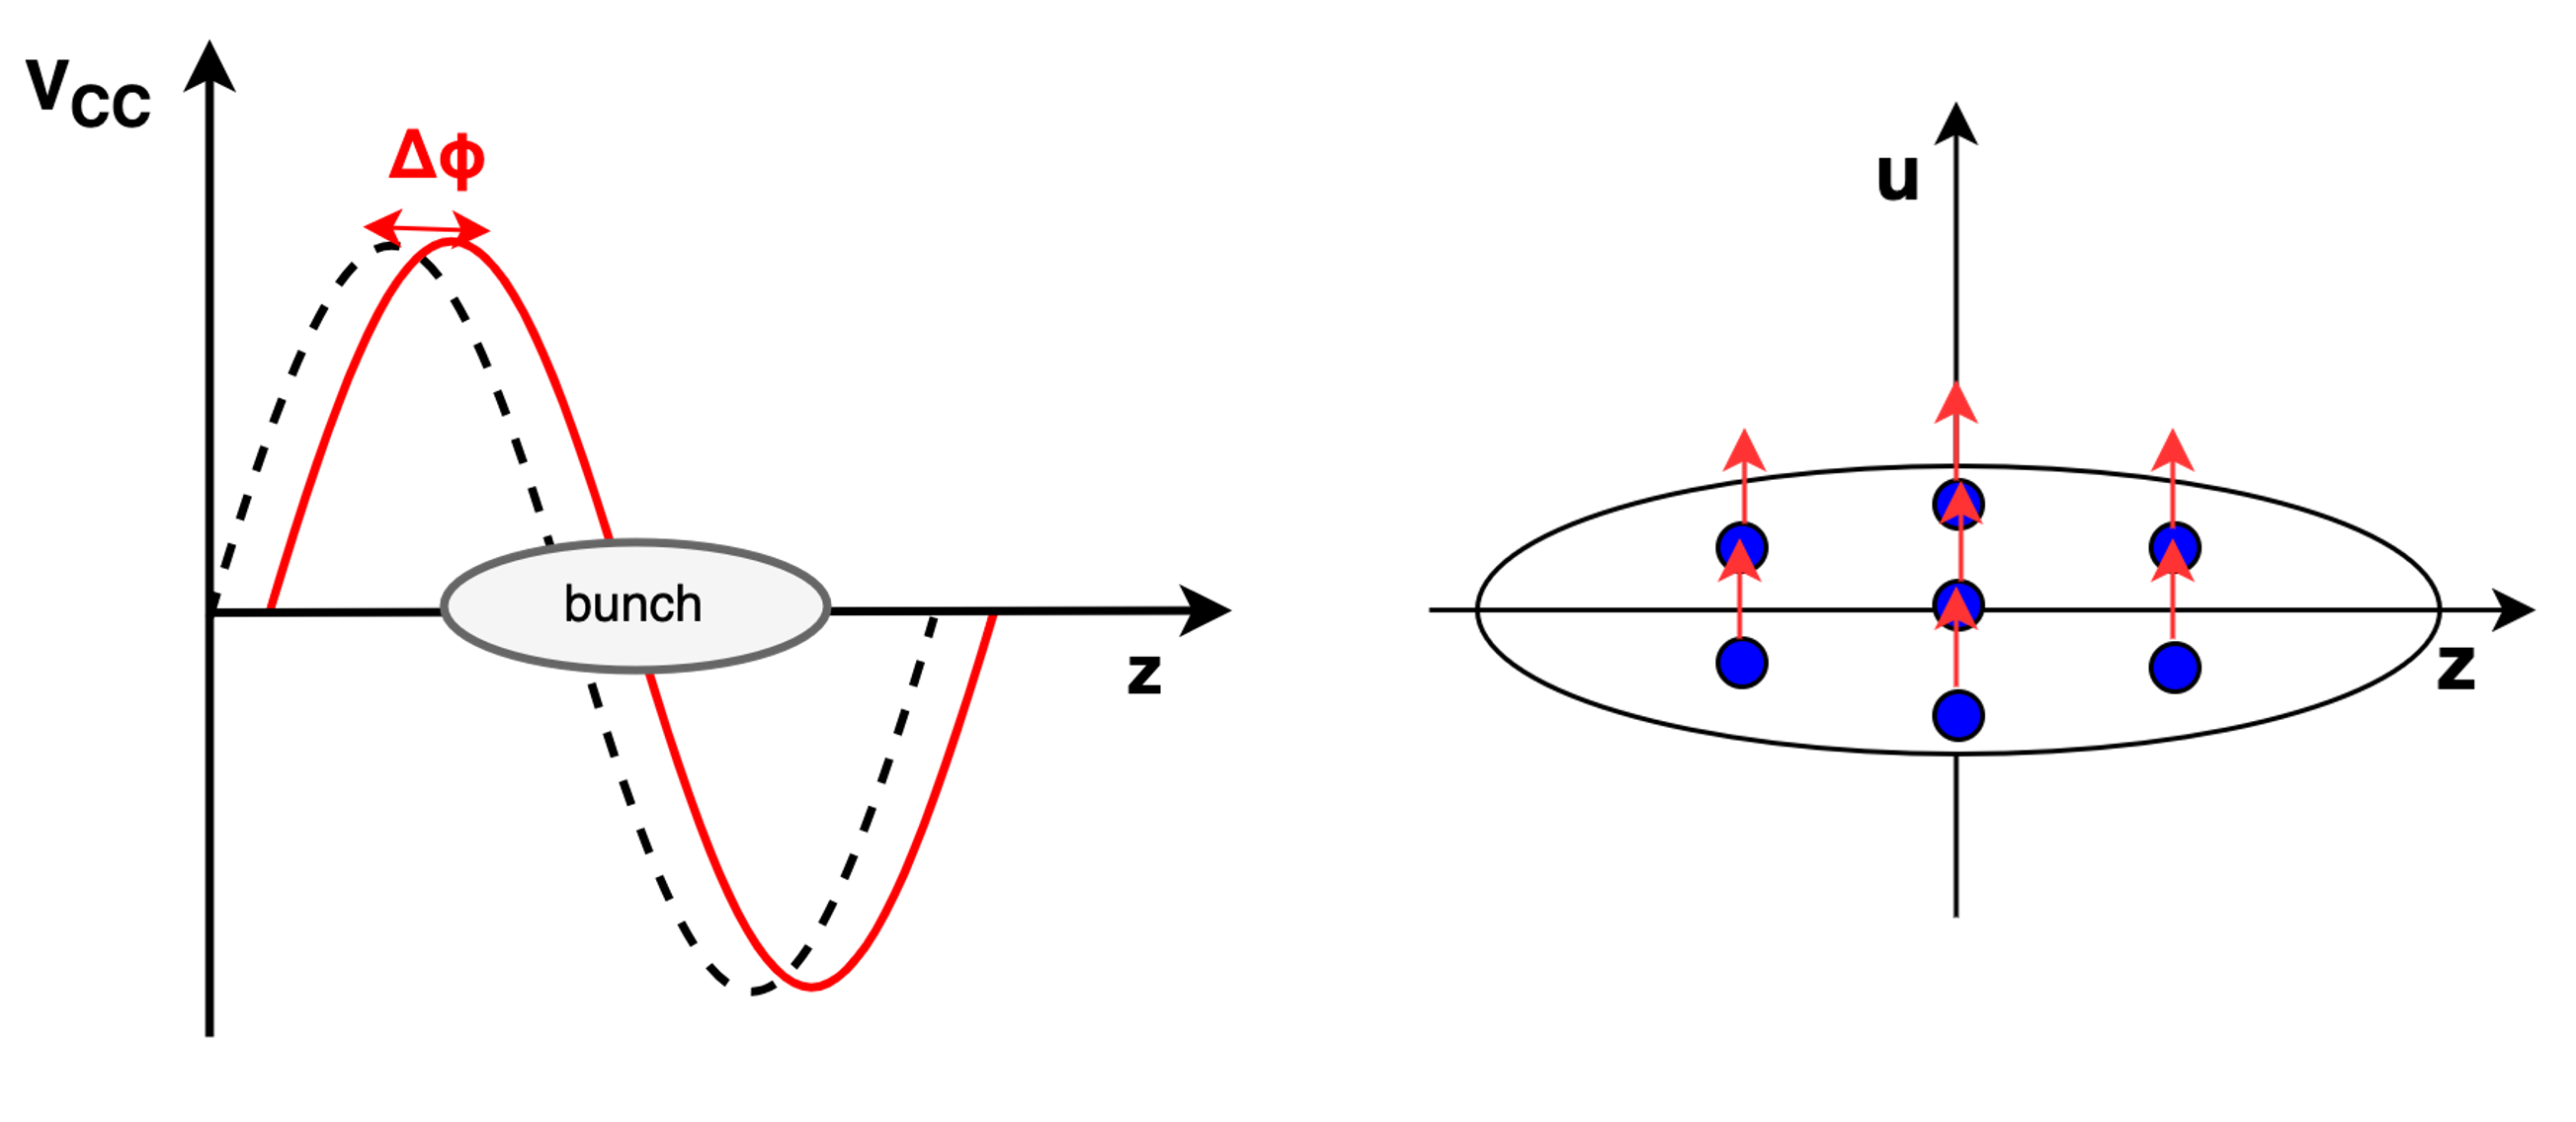
\includegraphics[width=0.8\textwidth]{images/Ch3/amplitude_noiser_merged.png}
        \caption{Modulation in amplitude or amplitude noise (left) and its impact on the particles within the bunch (right). The blue dots represent the individual particles while the red arrows indicate the direction of the noise kicks which act on them.}
        \label{fig:amplitude_noise}
 \end{figure}

 \begin{figure}[!h] % at the directory of ipac22
    \centering         
    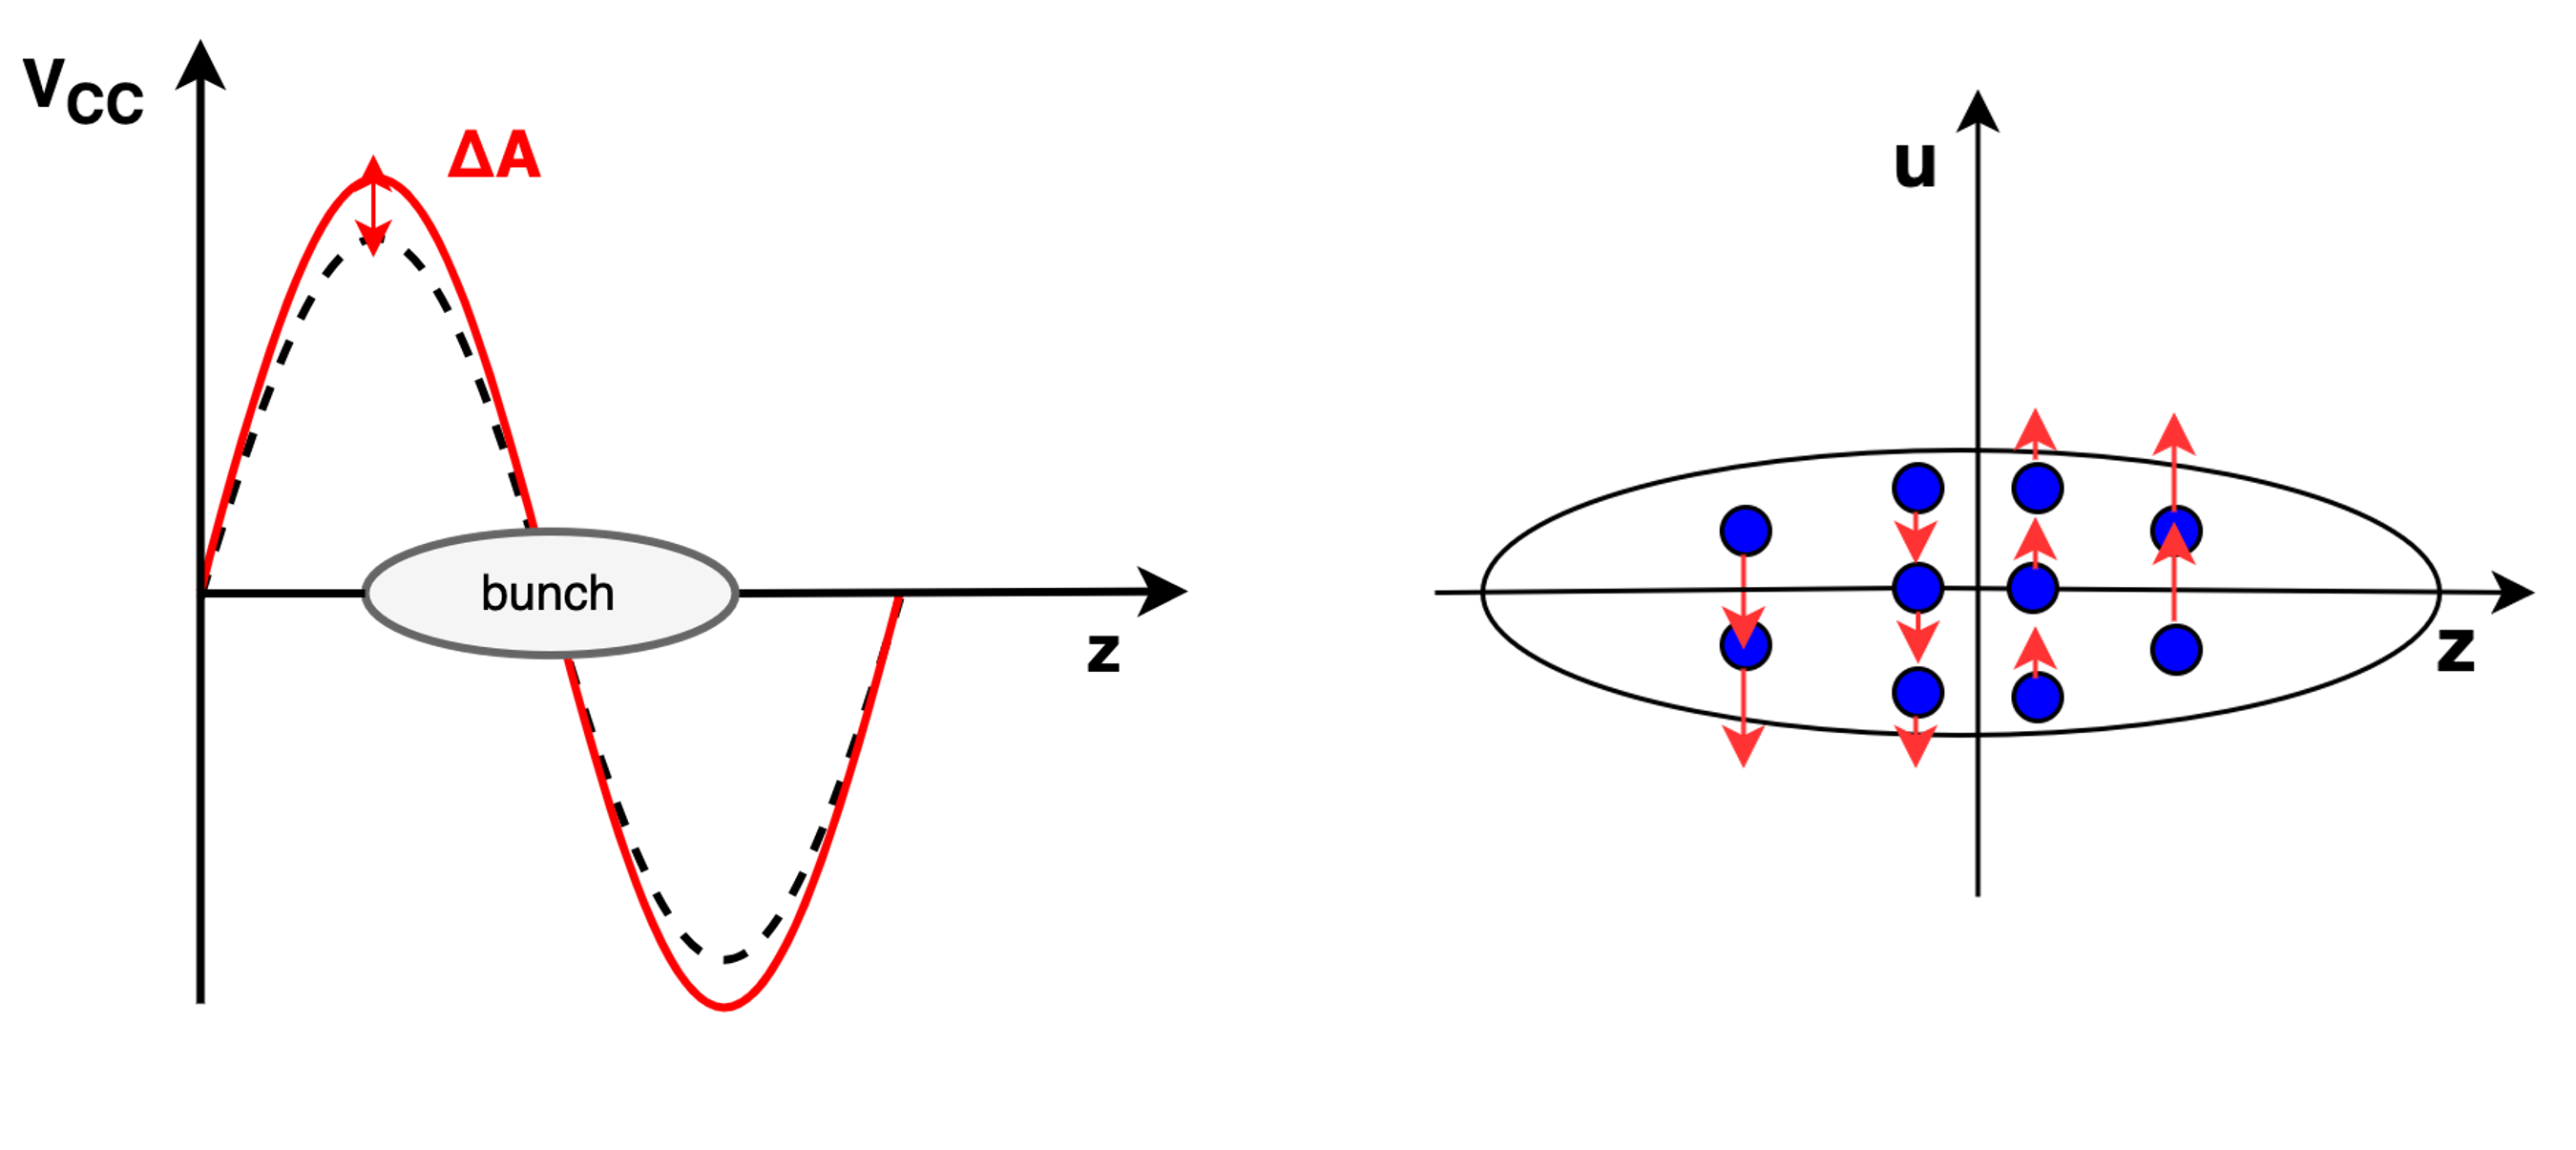
\includegraphics[width=0.85\textwidth]{images/Ch3/phase_noise_merged.png}
        \caption{Modulation in phase or phase noise (left) and its impact on the particles within the bunch (right). The blue dots represent the individual particles while the red arrows indicate the direction of the noise kicks which act on them.}
        \label{fig:phase_noise}
 \end{figure}

 Finally, it is worth mentioning, that for the LHC, HL-LHC and SPS $\CC$s the amplitude and phase RF noise are represented by white noise spectra. In that case, they can be considered as a sequence of uncorrelated random variables taken from a Gaussian distribution with zero mean and standard deviation $\sigma_{\Delta A}$ and  $\sigma_{\Delta \phi}$ respectively. The variances,  $\sigma_{\Delta A}^2$ and  $\sigma_{\Delta \phi}^2$ equal the total noise power (see Appendix~\ref{app:discrete_time_analysis} for definitions). % sampled by the beam, as also written here: https://www.osti.gov/servlets/purl/1846026 

\subsection{Emittance growth formulas}\label{subsec:CC_emit_growth_theoretical_formulas}
As already mentioned, the theoretical formalism for predicting the transverse emittance growth in the presence of $\CC$ RF amplitude and phase noise was derived in Ref.~\cite{PhysRevSTAB.18.101001}. The derivation assumes: single bunch crossing the crab cavity with zero phase at $z=0$; no horizontal-vertical coupling; constant energy (no acceleration). The noise kicks are represented as a stochastic process with uniform spectrum across the betatron tune distribution.

%a single bunch, that the noise kicks are represented by a stochastic process, zero coupling between the horizontal and vertical plane, the beam energy is constant (no acceleration) and, $\CC$ RF zero phase is at the center of the bunch, $z=0$ and a uniform noise spectrum across the betatron tune distribution which is also symmetric in negative and positive frequencies. 
% One more assumption that I didn't write Inthe analysis presented in this work, the density function is independent of time (paper of themis and philippe p.2) i didn't write it in the assumption.

Taking these conditions into account, the emittance growth resulting from amplitude noise is estimated from:
\begin{equation}\label{eq:dey_an}
    \frac{d\epsilon^{\mathrm{geom}}_u}{dt}  = \beta_{u, \mathrm{CC}} \left( \frac{e\CCvoltage\frev}{2E_b}\right)^2 \!\! C_{\Delta A} (\sigma_{\phi}) \!\! \sum_{k=-\infty}^{+\infty} S_{\Delta A}[(k \pm \widebar{q}_u \pm \widebar{q}_s)\frev].
\end{equation}
For phase noise, the emittance growth is estimated from:
\begin{equation}\label{eq:dey_pn}
    \frac{d\epsilon^{\mathrm{geom}}_u}{dt}  = \beta_{u, \mathrm{CC}}  \left( \frac{e\CCvoltage\frev}{2E_b}\right)^2 C_{\Delta \phi} (\sigma_{\phi}) \sum_{k=-\infty}^{+\infty} S_{\Delta \phi}[(k \pm \widebar{q}_u) \frev].
\end{equation}
In these formulas, which are valid for both transverse planes as $u=(x,y)$, $\beta_{u, \mathrm{CC}}$ is the transverse beta function at the location of the CC, $\CCvoltage$ the CC voltage, $\frev$ the revolution frequency of the beam, $E_b$ the beam energy, and $\widebar{q}_u$ and $\widebar{q}_s$ the mean of the betatron and synchrotron tune distribution \footnote{For white noise spectra the effect of noise is independent of the actual tune distribution, hence the use of the mean quantities. The generic formulas can be found in Ref.~\cite{PhysRevSTAB.18.101001}} where $q_u, q_s$ (with lower case) denote the fractional part of the betatron and synchrotron tunes respectively. $S_{\Delta A}$ and $S_{\Delta \phi}$ are the power spectral densities (PSD) of the noise at all the betatron and synchrobetatron (for the amplitude noise case) sidebands and they are expressed in units of Hz$^{-1}$ and rad$^2$Hz$^{-1}$, respectively. In particular, $k \in \mathbb{Z}$ is the harmonic number of the revolution frequency and the $\pm$ signs refer to the upper $(+)$ and lower $(-)$ sidebands at each multiple of the revolution frequency, $k f_\mathrm{rev}$.%, from the betatron tune.

The definition of the power spectral density along with the fundamental terminology for the signal-processing can be found in Appendix~\ref{ch:app_B}. %\footnote{In the Appendix amplitude and phase noise are noted with just $\alpha$ and $\phi$, instead of $\Delta A$ and $\Delta \phi$, for simplicity.}. 
As all the studies presented in this thesis, are done with white noise the power spectral densities can be computed using Eqs.~\eqref{eq:psd_for_white_noise_variance_AN} and~\eqref{eq:psd_for_white_noise_variance_PN} introduced earlier.


The terms $C_{\Delta A}$ and $C_{\Delta \phi}$ are correction terms to account for the bunch length:
\begin{align}
C_{\Delta A}(\sigma_{\phi}) = ~& e^{-\sigma_{\phi}^2}\sum_{l=0}^{+\infty} I_{2l+1}(\sigma_{\phi}^2),\\
C_{\Delta \phi}(\sigma_{\phi}) = ~& e^{-\sigma_{\phi}^2} \left[I_0(\sigma_{\phi}^2) + 2 \sum_{l=1}^{+\infty} I_{2l}(\sigma_{\phi}^2) \right],
\end{align}
with $\sigma_{\phi}$ the rms bunch length, in radians, with respect to the CC frequency $\CCfrequency$, and $I_n(x)$ the modified Bessel function of the first kind. 

Figure~\ref{fig:correction_term_bunch_length} illustrates the correction term for different values of bunch length for amplitude (left) and phase (right) noise. The SPS nominal bunch length used in the CC tests is shown as an orange dot for reference.

% Figures created using the following script: natriant/cernbox/Project_thesis/plot_bunch_length_correction_term
\begin{figure}[!ht]
    \centering
    \begin{subfigure}[t]{0.45\textwidth}
        \centering
        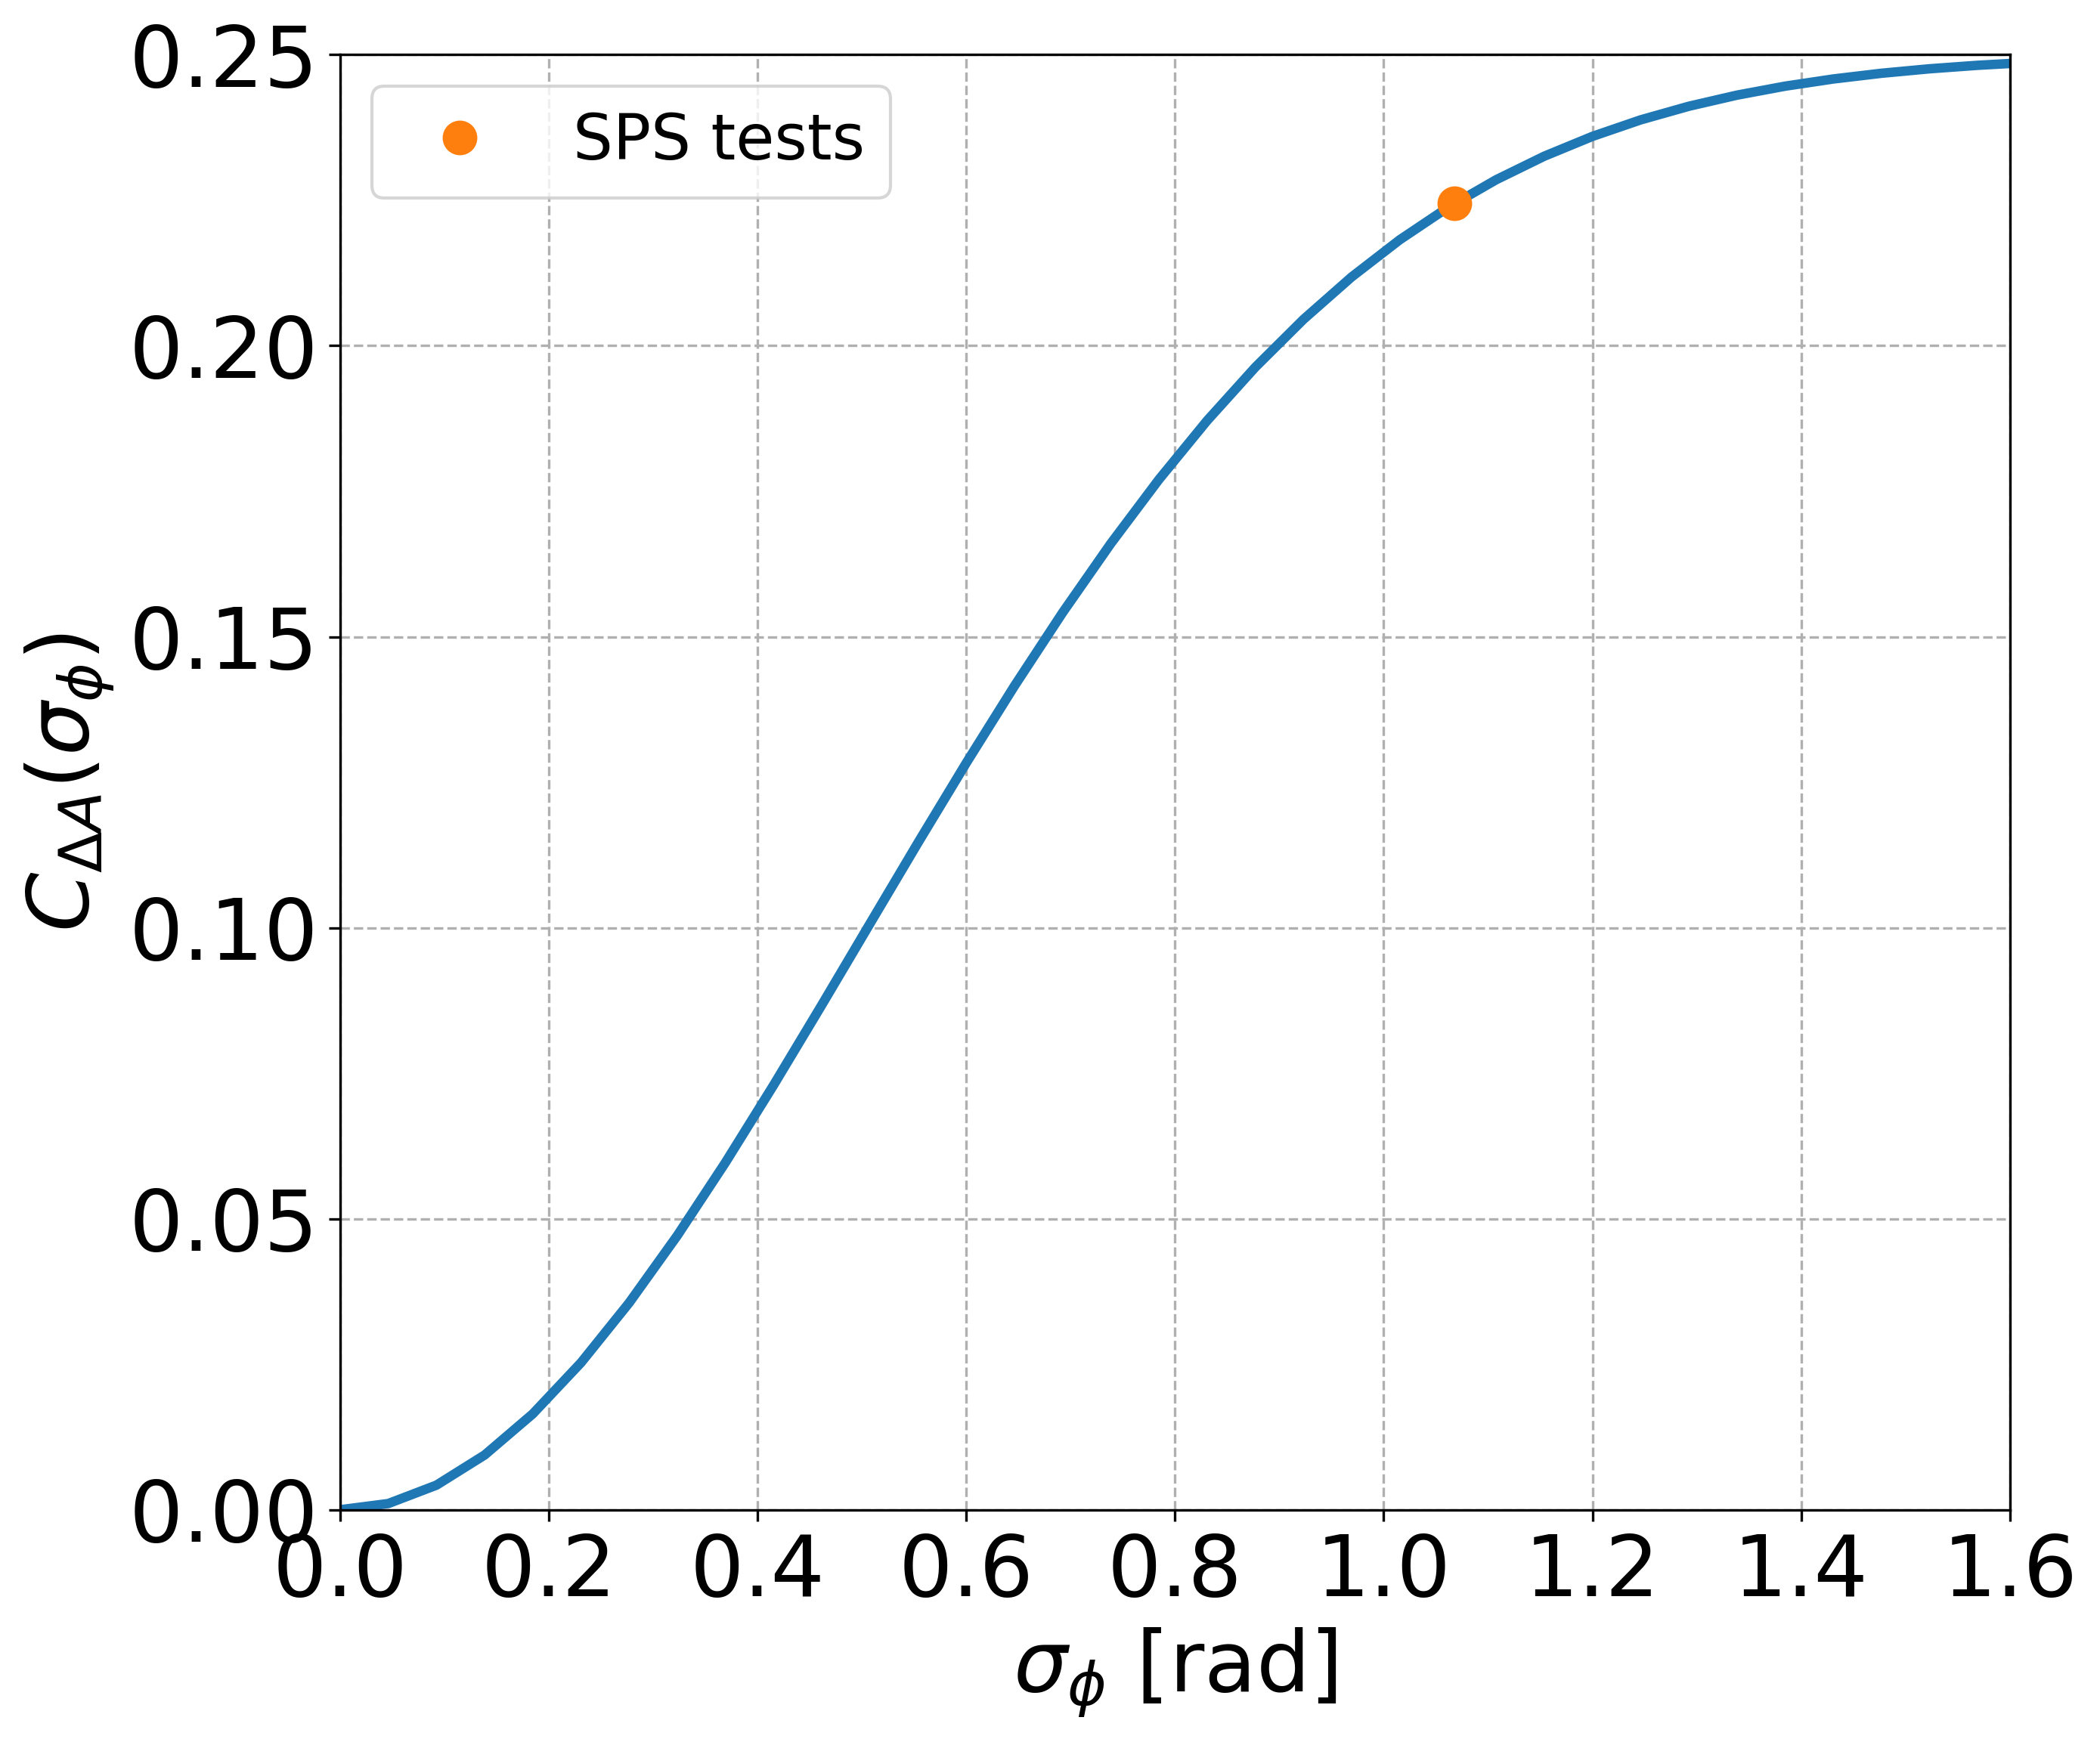
\includegraphics[width=1\textwidth]{images/Ch3/CA_bunch_length_dependence.png}
        %\caption{$y=\sin(2 \pi f t),\ f=50$ Hz}
        %\label{fig:add_label_here}
    \end{subfigure}
    \hfill
    \begin{subfigure}[t]{0.45\textwidth}
        \centering
        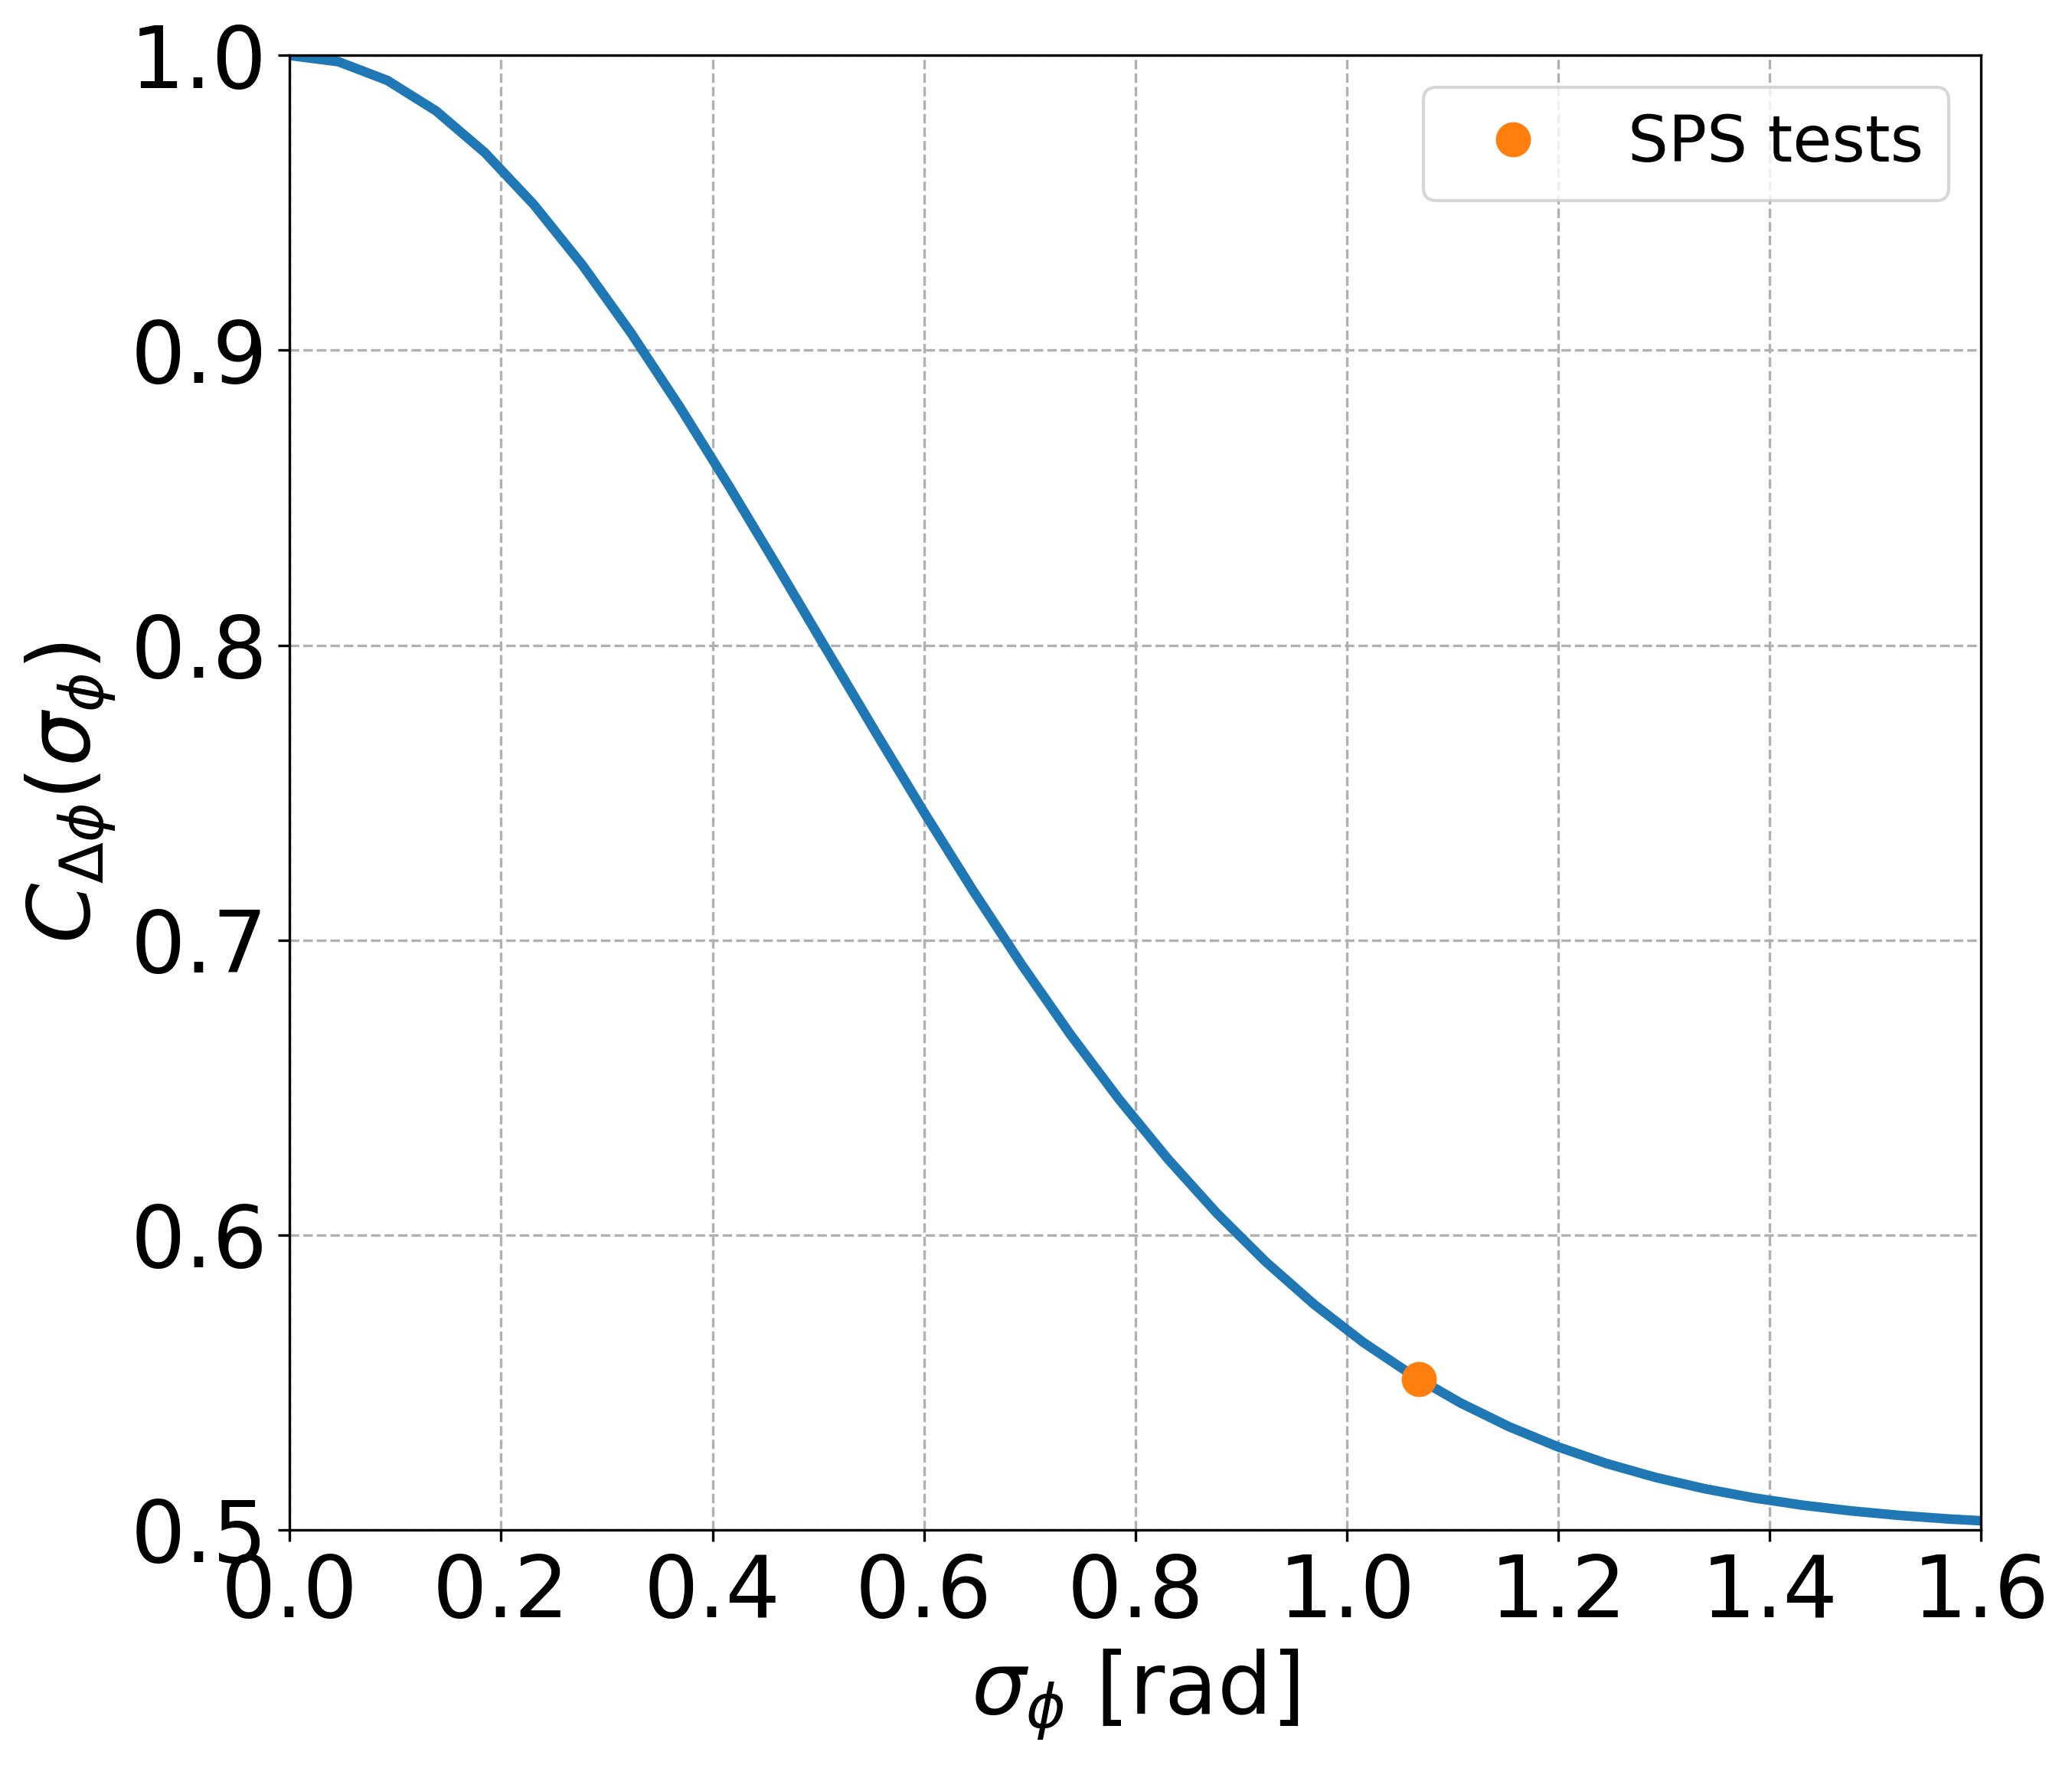
\includegraphics[width=1\textwidth]{images/Ch3/Cphi_bunch_length_dependence.png}
        %\caption{Discrete Fourier transform}
        %\label{fig:add_label_here}
    \end{subfigure}
    \hfill
     \caption{Correction term for amplitude (left) and phase (right) noise over a range of bunch length values.} % bunch passage
     \label{fig:correction_term_bunch_length}
 \end{figure}

\textbf{Comment on the use of the emittane growth formulas}\\
Here some additional comments on the use of the Eq.~\eqref{eq:dey_an} and Eq.~\eqref{eq:dey_pn} for predicting the emittance growth rate for both measurements and simulation studies of this thesis are made to facilitate the discussion in the following chapters.

In this thesis, the emittance growth in the vertical plane is addressed. The reason is that for both experimental campaigns that took place in 2018 and 2022, the $\CC$ module (DQW) that was available provided a vertical deflection on the beam. For reference, the $\CC$ module which provides horizontal deflection (RFD) is planned to be available by the end of 2022. Additionally the studies were performed for the SPS machine for which the parameters are listed in Table~\ref{tab:machine_beam_param_2018}: $q_y=0.18$, $f_\mathrm{rev}=43.38$\,kHz, and $q_s=0.0051$. 

To this end, the emittance growth induced by $\CC$ RF noise depends on the power spectral density value of the noise at the vertical betatron and synchrobetatron sidebands for the phase and amplitude noise case respectively (see Eq.~\eqref{eq:dey_an} and Eq.~\eqref{eq:dey_pn}). The upper and lower sidebands of the first and second vertical betatron sidebands are observed in the following frequencies:
\begin{equation}\label{eq:betatron_sideband_1}
    \mathrm{k=0}: \ (0 \pm \widebar{q}_y) f_\mathrm{rev} = \pm 0.18 \times 43.38\mathrm{\,kHz} \approx \pm 7.8\mathrm{\,kHz}.
\end{equation}
\begin{equation}\label{eq:betatron_sideband_2}
    \mathrm{k= \pm 1}: \ (\pm 1 \pm \widebar{q}_y) f_\mathrm{rev} = (\pm 1 \pm 0.18) \times 43.38\mathrm{\,kHz} \approx \begin{dcases*} 
        \text{$-$51.2\,kHz and $-$35.6\,kHz,} & if  $k=-1$ \\ 
        \text{51.2\,kHz and 35.6\,kHz,} & if  $k=1$  
        \end{dcases*} .
\end{equation}

The upper and lower sidebands of the first and second vertical synchrobetatron sidebands are observed in the following frequencies:
\begin{equation}\label{eq:synchrobetatron_sideband_1}
    \mathrm{k=0}: \ (0 \pm \widebar{q}_y \pm \widebar{q}_s) f_\mathrm{rev} = (\pm 0.18 \pm 0.0051) \times 43.38\mathrm{\,kHz} \approx \pm 8.02\mathrm{\,kHz} \ \mathrm{and} \pm 7.6\mathrm{\,kHz}.
\end{equation}
\begin{equation}\label{eq:synchrobetatron_sideband_2}
    \begin{split}
    \mathrm{k= \pm 1}: \ (\pm 1 \pm \widebar{q}_y \pm \widebar{q}_s) f_\mathrm{rev} = (\pm 1 \pm 0.18 \pm 0.0051)\times 43.38\mathrm{\,kHz} \approx \\ 
    \approx \begin{dcases*} 
        \text{$-$35.35, $-$35.79, $-$50.96, $-$51.40\,kHz,} & if  $k=-1$ \\ 
        \text{35.35, 35.79, 50.96, 51.40\,kHz,} & if  $k=1$  
        \end{dcases*} .
    \end{split}
\end{equation}


The experimental studies with $\CC$s (more details in Chapter~\ref{Ch:2018_analyisis}) were conducted with an artificial noise spectrum which was up to 10\,kHz, which as it becomes clear from the Eqs.~\eqref{eq:betatron_sideband_1}-~\eqref{eq:synchrobetatron_sideband_2} is overlapping and therefore exciting only the first betatron and synchrobetatron sidebands, $k=0$ (upper and lower).

In the simulations, the beam particles encounter the phase or amplitude noise kicks once per turn. This means that the sampling frequency of the noise spectrum in the frequency domain equals, $f_s=f_\mathrm{rev}=43.38$\,kHz. This means, that the frequency spectrum of the noise applied in the simulations extends from $-f_s/2 \approx -22$\,kHz to $+f_s/2 \approx 22$\,kHz. \footnote{The particles will still be affected by noise above the Nyquist frequency, $\frev /2$ but up to $\frev$ (if there are any betatron and/or synchrobetatron sidebands in that range), but the noise will alias into lower frequencies. This is not the case for the studies presented in this thesis, as it becomes evident from Eqs.~\eqref{eq:betatron_sideband_1}-~\eqref{eq:synchrobetatron_sideband_2}.} Further explanation can be found in Appendix~\ref{ch:app_B} and specifically in the Section~\ref{subsec:generatin_noise_kicks}. Again, from Eqs.~\eqref{eq:betatron_sideband_1}-~\eqref{eq:synchrobetatron_sideband_2} it becomes clear that the noise kicks in the simulations excite only the first betatron and synchrobetatron sidebands for $k=0$ (upper and lower).

To sum up, when using Eqs.~\eqref{eq:dey_an} and~\eqref{eq:dey_pn} to predict the emittance growth rate due to $\CC$ RF noise in the SPS, $k=0$ will be considered.

\section{Studies in KEKB}\label{eq:past_studies_KEKB}
$\CC$s have been tested in the past with lepton beams in KEKB in Japan (further references on their operation are given in~\cite{CC_KEKB_4440798, Funakoshi:1955812, oide:pac07-mozaki01}). %~\cite{CC_KEKB_4440798, Funakoshi:1955812, oide:pac07-mozaki01}.
The tests included studies of the effects on the beam of RF noise in the $\CC$s. However, there were significant differences in KEKB, compared to SPS, LHC and HL-LHC In particular, the studies in KEKB were conducted for lepton bunches, rather than hadron bunches.  The bunch length in KEKB was smaller by an order of magnitude than in SPS or HL-LHC: this means that the effects of amplitude noise would be negligible in KEKB.  Furthermore, synchrotron radiation in lepton storage rings provides significant damping.  Finally, the RF noise in KEKB was characterised by a single spectral line, rather than white noise. Due to these differences, the studies at KEKB are not applicable to the studies presented in this thesis. These studies can be found in Ref.~\cite{PhysRevSTAB.14.111003}: they provide the only previous experience with crab cavity operation in storage rings, but because of the differences with SPS and HL-LHC, further details of the KEKB studies are beyond the scope of this thesis



Now that the theoretical formulas for the $\CC$ RF noise-induced emittance growth have been introduced, they will be used through the following chapters for comparison against numerical simulations and experimental measurements (in the SPS) for developing confidence in the theoretical model and its predictions for the HL-LHC.


\chapter{Calibration of the Crab Cavities for the SPS tests in 2018}\label{Ch:CC_set_up}
In 2018, two prototype Crab Cavities (CCs) were installed in the SPS to be tested for the first time
with proton beams. One of the operational issues that needed to be addressed concerned the expected 
emittance growth due to noise in their RF control system. A theoretical model had already been developed
and validated by tracking simulations~\cite{PhysRevSTAB.18.101001}. Based on those studies a dedicated 
experiment was performed to benchmark the models with experimental data and to confirm the analytical
 predictions. In particular, the idea was to inject various noise levels in the CC RF system and record
 the emittance evolution. In this chapter, the measurement results from the experiment are presented 
 and discussed. 

\chapter{Experimental studies 2018: emittance growth from Crab Cavity noise}\label{Ch:2018_setup}
In 2018, two prototype Crab Cavities ($\CC$s) were installed in the SPS to be tested for the first time with proton beams. One of the operational issues that needed to be addressed concerned the expected emittance growth due to noise in their RF control system. A theoretical model that describes this emittance growth had already been developed and validated by tracking simulations~\cite{PhysRevSTAB.18.101001}. Based on those studies a dedicated experiment was performed to benchmark the models with experimental data and to confirm the analytical predictions. In particular, the idea was to inject various noise levels in the $\CC$ RF system and record the emittance evolution. In this chapter, the experimental procedure, the measurement methods and results are presented and discussed.
 
The chapter is stractured as follows: Section~\ref{sec:CC_SPS_setup} describes the operational setup for the SPS $\CC$ tests and discusses the main diagnostic deployed for the derivation of the $\CC$ voltage.

blah blah ... describe sections and subsections after they are completed.

blah blah ... describe sections and subsections after they are completed.

blah blah ... describe sections and subsections after they are completed.

\section{Crab Cavities in the SPS}\label{sec:CC_SPS_setup}

For the SPS tests two prototype $\CC$s of the Double Quorter Wave (DQW) type were fabricated by CERN and were assembled into the same cryomodule~\cite{Zanoni:2017}. The cryomodule was installed in the SPS-LSS6 zone and was placed on a mobile transfer table~\cite{Garlaschè:2648553}. The table moved with high precision and without breaking the vaccum the cryomodule in the beam line for the $\CC$ tests and out of it for the usual SPS operation. For the emittance growth measurements only one of these $\CC$s was used and its main optics and desgin parameters are listed in Table~\ref{tab:SPS_CCs}. 

%\chapter{Emittance growth studies 2018: Operational setup/preparation and beam instrumentation}\label{Ch:2018_setup}
%In 2018, two prototype Crab Cavities ($\CC$s) were installed in the SPS to be tested for the first time with proton beams. One of the operational issues that needed to be addressed concerned the expected emittance growth due to noise in their RF control system. A theoretical model that describes this emittance growth had already been developed and validated by tracking simulations~\cite{PhysRevSTAB.18.101001}. Based on those studies a dedicated experiment was performed to benchmark the models with experimental data and to confirm the analytical predictions. In particular, the idea was to inject various noise levels in the $\CC$ RF system and record the emittance evolution. In this chapter, the experimental procedure, the measurement methods and results are presented and discussed.
 
The chapter is stractured as follows: Section~\ref{sec:CC_SPS_setup} describes the operational setup for the SPS $\CC$ tests and discusses the main diagnostic deployed for the derivation of the $\CC$ voltage.

blah blah ... describe sections and subsections after they are completed.

blah blah ... describe sections and subsections after they are completed.

blah blah ... describe sections and subsections after they are completed.

\section{Crab Cavities in the SPS}\label{sec:CC_SPS_setup}

For the SPS tests two prototype $\CC$s of the Double Quorter Wave (DQW) type were fabricated by CERN and were assembled into the same cryomodule~\cite{Zanoni:2017}. The cryomodule was installed in the SPS-LSS6 zone and was placed on a mobile transfer table~\cite{Garlaschè:2648553}. The table moved with high precision and without breaking the vaccum the cryomodule in the beam line for the $\CC$ tests and out of it for the usual SPS operation. For the emittance growth measurements only one of these $\CC$s was used and its main optics and desgin parameters are listed in Table~\ref{tab:SPS_CCs}. 

\chapter{Emittance growth studies 2018: Measurements and analysis}\label{Ch:2018_analyisis}
\section{Parametric studies based on the theoretical model}\label{sec:paramteric_studies_theory}
% Link to presentations: https://docs.google.com/presentation/d/1wqgJK7uDFDGoX8gyx2-JhnO8mZT51N1VH1RtNL-jhWA/edit#slide=id.ga69ead34aa_0_419

The basics of the existing theoretical model which describes the emittance growth in the presence of amplitude and phase noise in the $\CC$s in a synchrotron have been introduced in Chapter~\ref{Ch:CC_noise_theory}. Here, this theory is used to study the sensitivity of the noise-induced emittance growth on the $\CC$ voltage and rms bunch length. The objective of the study is to investigate if the uncertainty in the measurements of these two variables could explain the observed discrepancy of a factor $\sim$4 between measured emittance growth and the analytically predicted values (see Section~\ref{sec:meas_2018_vs_theory}).
% The study is limited in these two parameters as they are the only measured ones that could introduce some incertainty in the Eqs. of phase and amplitude noise. In reality there is also some uncertaninty on the noise levels themselves but is not treated here. Nevertheless, extended studies on the noise spectrum are presented later in this section.

The following parametric studies were performed for the experimental configuration of 2018: beam energy of 270\,GeV, vertical beta function of 73\,m (at the location of $\CC$2), and phase and amplitude noise of -111.4 and -115.7\,dBc/Hz respectively (Coast2-Setting2). The phase and amplitude noise are considered here independently, instead of the effective phase noise, due to the different dependence of the correction term (see Fig.~\ref{fig:correction_term_bunch_length}).

\subsection{Sensitivity to bunch length}\label{subsec:bunch_length_dependence}
Using Eqs.~\eqref{eq:dey_an} and~\eqref{eq:dey_pn} with the above mentioned parameters and CC votlage, $V_\mathrm{CC}$=1\,MV the normalised vertical emittance growth is computed as a function of different values of bunch lengths over a range from $10^{-3}$ to 2.5\,ns (expressed in $4\sigma_t$). The results are illustrated in Fig.~\ref{fig:sensitivity_bunch_length_theory_bunch1}. 

A clear dependence of the vertical emittance growth on the bunch length is observed. However, the dependence is strong for short bunches. In the regime of the measured bunch length during the CC experiment for bunch 1 (~1.6ns-2.0ns) the sensitivity to the bunch length is very small and cannot explain the factor of about 4 that was observed between measurements and simualtions in SPS $\CC$ tests in 2018.

% Plotting script: Requires python 3
% https://github.com/natriant/theoreticalModel_for_emitGrowth_due2CCNoise/blob/master/cmpt_GrowthDependence_on_BunchLength_003_for_thesis.py
\begin{figure}[!h]
    \centering         
    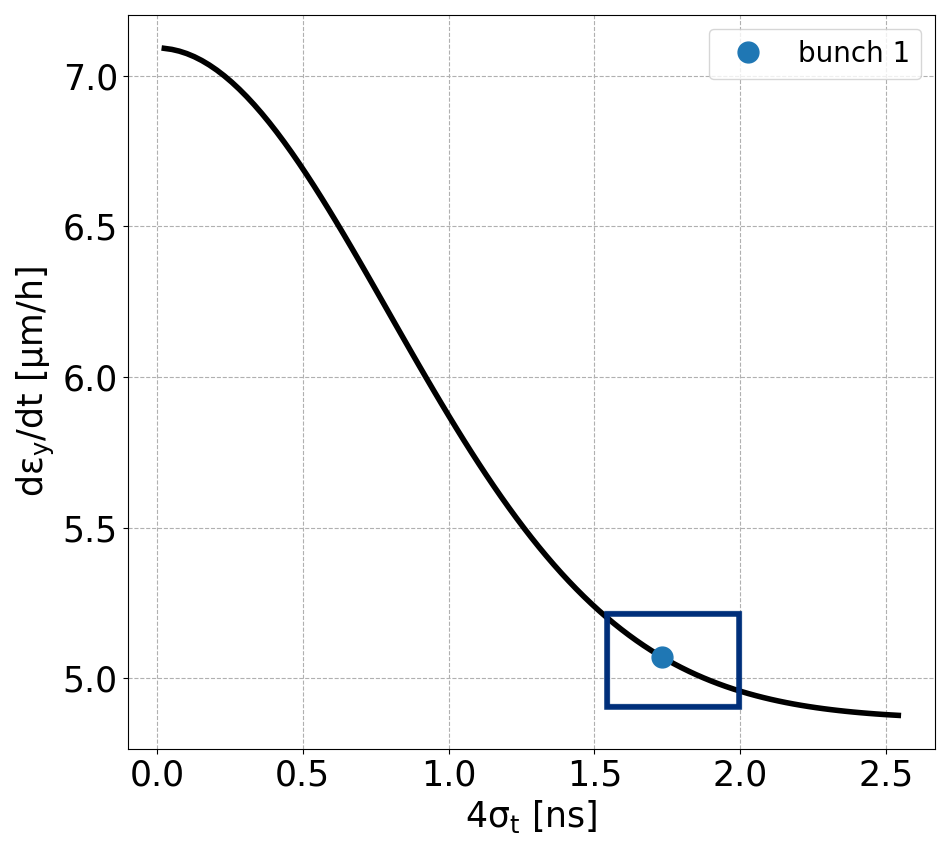
\includegraphics[width=0.7\textwidth]{images/Ch6/dey_vs_4sigmat_Coast2-Setting2_withBunches_v2.png}
        \caption{Vertical emittance growth for different bunch length values computed using the analytical formulas Eqs.~\eqref{eq:dey_an} and~\eqref{eq:dey_pn} for the experimental configuration of 2018. The blue dot shows the average rms bunch length over all coasts in 2018. The blue box around it gives the upper and lower limits of its measurements.}
        \label{fig:sensitivity_bunch_length_theory_bunch1}
 \end{figure}


\subsection{Sensitivity to CC voltage}\label{subsec:bunch_length_dependence}
Here, the sensitivity of the vertical emittance growth is studied for the parameters mentioned above and rms bunch length of $4\sigma_t=$1.7\,ns. The vertical emittance growth is computed again analytically using Eqs.~\eqref{eq:dey_an} and~\eqref{eq:dey_pn} over a range of $\CC$ voltage values equally spaced from 0.6 to 1.3\,MV. 

Figure~\ref{fig:sensitivity_VCC_theory_bunch1} illustrates the computed vertical emittance as a function of the CC voltage. From the analysis in 2018, the calibration of the CC voltage which showed 1\,MV was tricky. However, from the plot it is evident that even if the actual voltage was 30$\%$ lower due to errors this would lead to just a factor of 2 lower vertical emittance growth. An error of this scale is not realistic. To this end, it is concluded that uncertainties on the beam based measurements of the CC voltage cannot explain the expereimental observations of 2018, where there was a factor 4 betewen measured and predicted emittance growth.

% Plotting script: Requires python 3
% https://github.com/natriant/theoreticalModel_for_emitGrowth_due2CCNoise/blob/master/cmpt_GrowthDependence_on_Vcc.py
\begin{figure}[!h]
    \centering         
    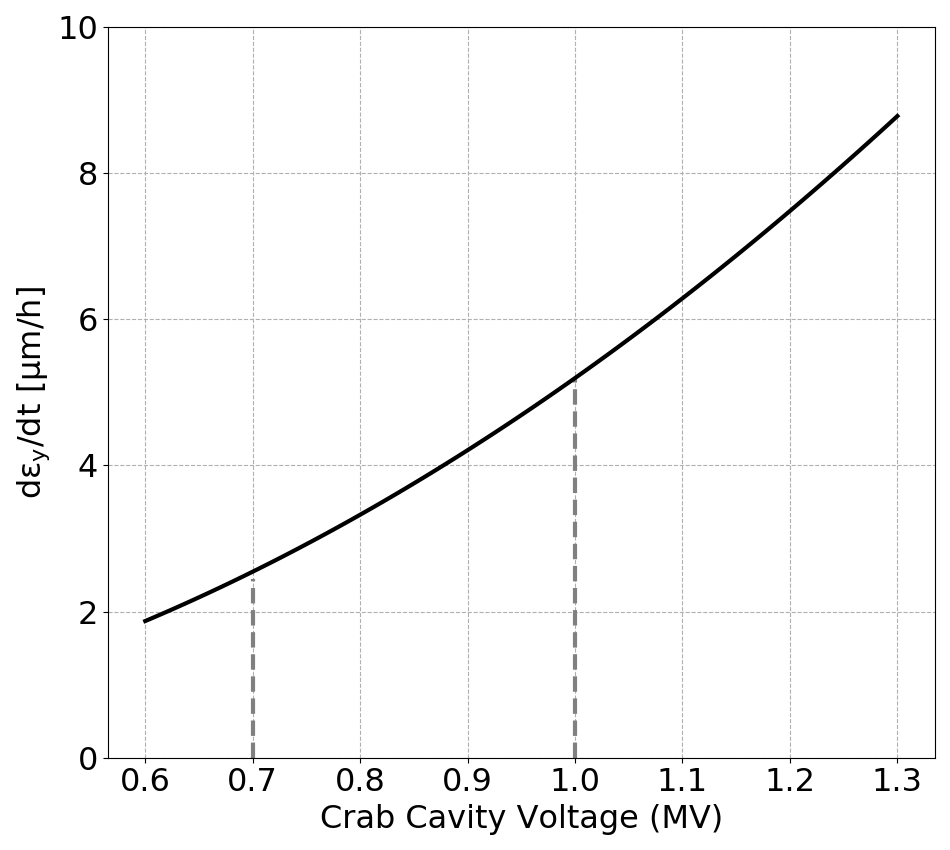
\includegraphics[width=0.7\textwidth]{images/Ch6/dey_vs_Vcc_Coast2-Setting2.png}
        \caption{Vertical emittance growth for different values of CC voltage computed using the analytical formulas Eq.~\eqref{eq:dey_an} and~\eqref{eq:dey_pn} for the experimental configuration of 2018.}
        \label{fig:sensitivity_VCC_theory_bunch1}
 \end{figure}






\newpage


for the experimental configuration of 2018 

of the existing Vlasov theory for transverse coherent beam instabilities with first-order
chromaticity have been recapitulated in Section 2.2.3. Here, we extend this theory to account for the
beam dynamics effects introduced by nonlinear chromaticity. The chapter contains the work published
in Refs. [34, 76].




\section{Benchmarking with different simulation software}
Benchmarking of theory with pyheadtail (one turn map) and Sixtracklib (element by element tracking).



\subsection{PyHEADTAIL}
- real CC element
- local vs global cc scheme
- How emittance is computed. No dipsersive contribution. studies vertical plane. \\
- It was verified in Sixtracklib simulations that the result from this simplified implementation is equivalent to the simulation with the true CC kick including phase noise.\\
- Need to say why in the simulations we have excitation of only the first betatron sideband. \\
\subsection{Sixtracklib}

Remember that in chapter 6 it was demonstrated that there is no visible difference on the cc rf noise induced emittance growth if the noise kicks are modeled as kicks on the moemntum or the real rf multiple + used in a global or local scheme.


pyheadtail vs sixtracklib: %https://docs.google.com/presentation/d/1rBVKGd9aBZTslaAHf48FdJkNPRyXtMF_T9XpEBlLE4c/edit#slide=id.g8ae11a254a_0_701

\section{Sensitivity to the non-linearities of the main SPS dipoles}
Simulation studies with sixtracklib

\section{Simulations using the measured noise spectrum}
Sixtracklib PyHEADTAIL and the exact machine paramters

\section{Sensitvity studies}
1. Sensitvity to how noisy is the noise spectrum
2. On the CC voltage
3. On the different bunch lengths. 

\section{b3b5b7 multiple errors}
Contribution of the non-linearities with sixtracklib.


All these factors were excluded as possible sources of the discrepancy.

\chapter{Investigation of the discrepancy}\label{Ch:investigating_discrepancy}

During the dedicated experiment that took place in the SPS
in 2018 with the CCs, the measured emittance
growth was found to be a factor four (on average) lower than
expected from the theory (see Section~\ref{sec:meas_2018_vs_theory}). The reason for this discrepancy remained unresolved for some time, as detailed follow-up studies (see Chapter~\ref{Ch:investigating_discrepancy}) investigated and excluded a number of possible explanations for the discrepancy.
It was recently found, that the beam transverse impedance, which is not included in the theory~\cite{PhysRevSTAB.18.101001} used for the comparison with the measurements may impact the noise-induced emittance growth and explain the experimental observations. Here, the damping mechanism from the beam transverse impedance is investigated as observed in detailed PyHEADTAIL simulations.

The structure of this chapter is as follows:




\section{SPS transverse impedance model}\label{sec:sps_impedance_model}
The PyHEADTAIL studies presented in this chapter are performed including the detailed transverse impedance model of the SPS machine~\cite{sps_impedance_model_git}. This model has been developed through a combination of theoretical computations, electromagentic simulations and was benchmarked with beam-based measurements~\cite{Salvant:1274254, Zannini:1561199, Salvant:1271349, Zannini:2141779}. 
It includes the contributions from all the individual elements in the SPS lattice i.e. the resistive wall, the indirect space charge, the kickers, the RF cavities (200\,MHz and 800\,MHz), the step transitions and the horizontal and vertical beam position monitors~\cite{Zannini:2141779}. As discussed in  Section~\ref{subsec:pyheadtail}, the model needs to represent the global impedance of the full machine. Thus, the total impedance is obtained by summing up the impedance of each element weighted with the beta function at its location and by dividing the sum by the average beta function of the SPS. For the Q26 optics the average horizontal and vertical beta functions are 42.09\,m and 42.01\,m respectively.
%https://indico.cern.ch/event/299470/contributions/686509/attachments/564150/777102/LIUSPS_transverse_imp_5.pdf
% The Wall contribution included both the resistive wall and the indirect SC.
Figure~\ref{fig:sps_impedance_model_H_V} shows the complete transverse impedance model of the SPS machine with the disentangled dipolar (blue) and quadrupolar (orange) terms to be plotted seperetaly. 

% Plot figures: /eos/user/n/natriant/Project_thesis/plot_wakefields_impedances_SPS
\begin{figure}[!ht]
    \centering
    \begin{subfigure}[t]{0.45\textwidth}
        \centering
        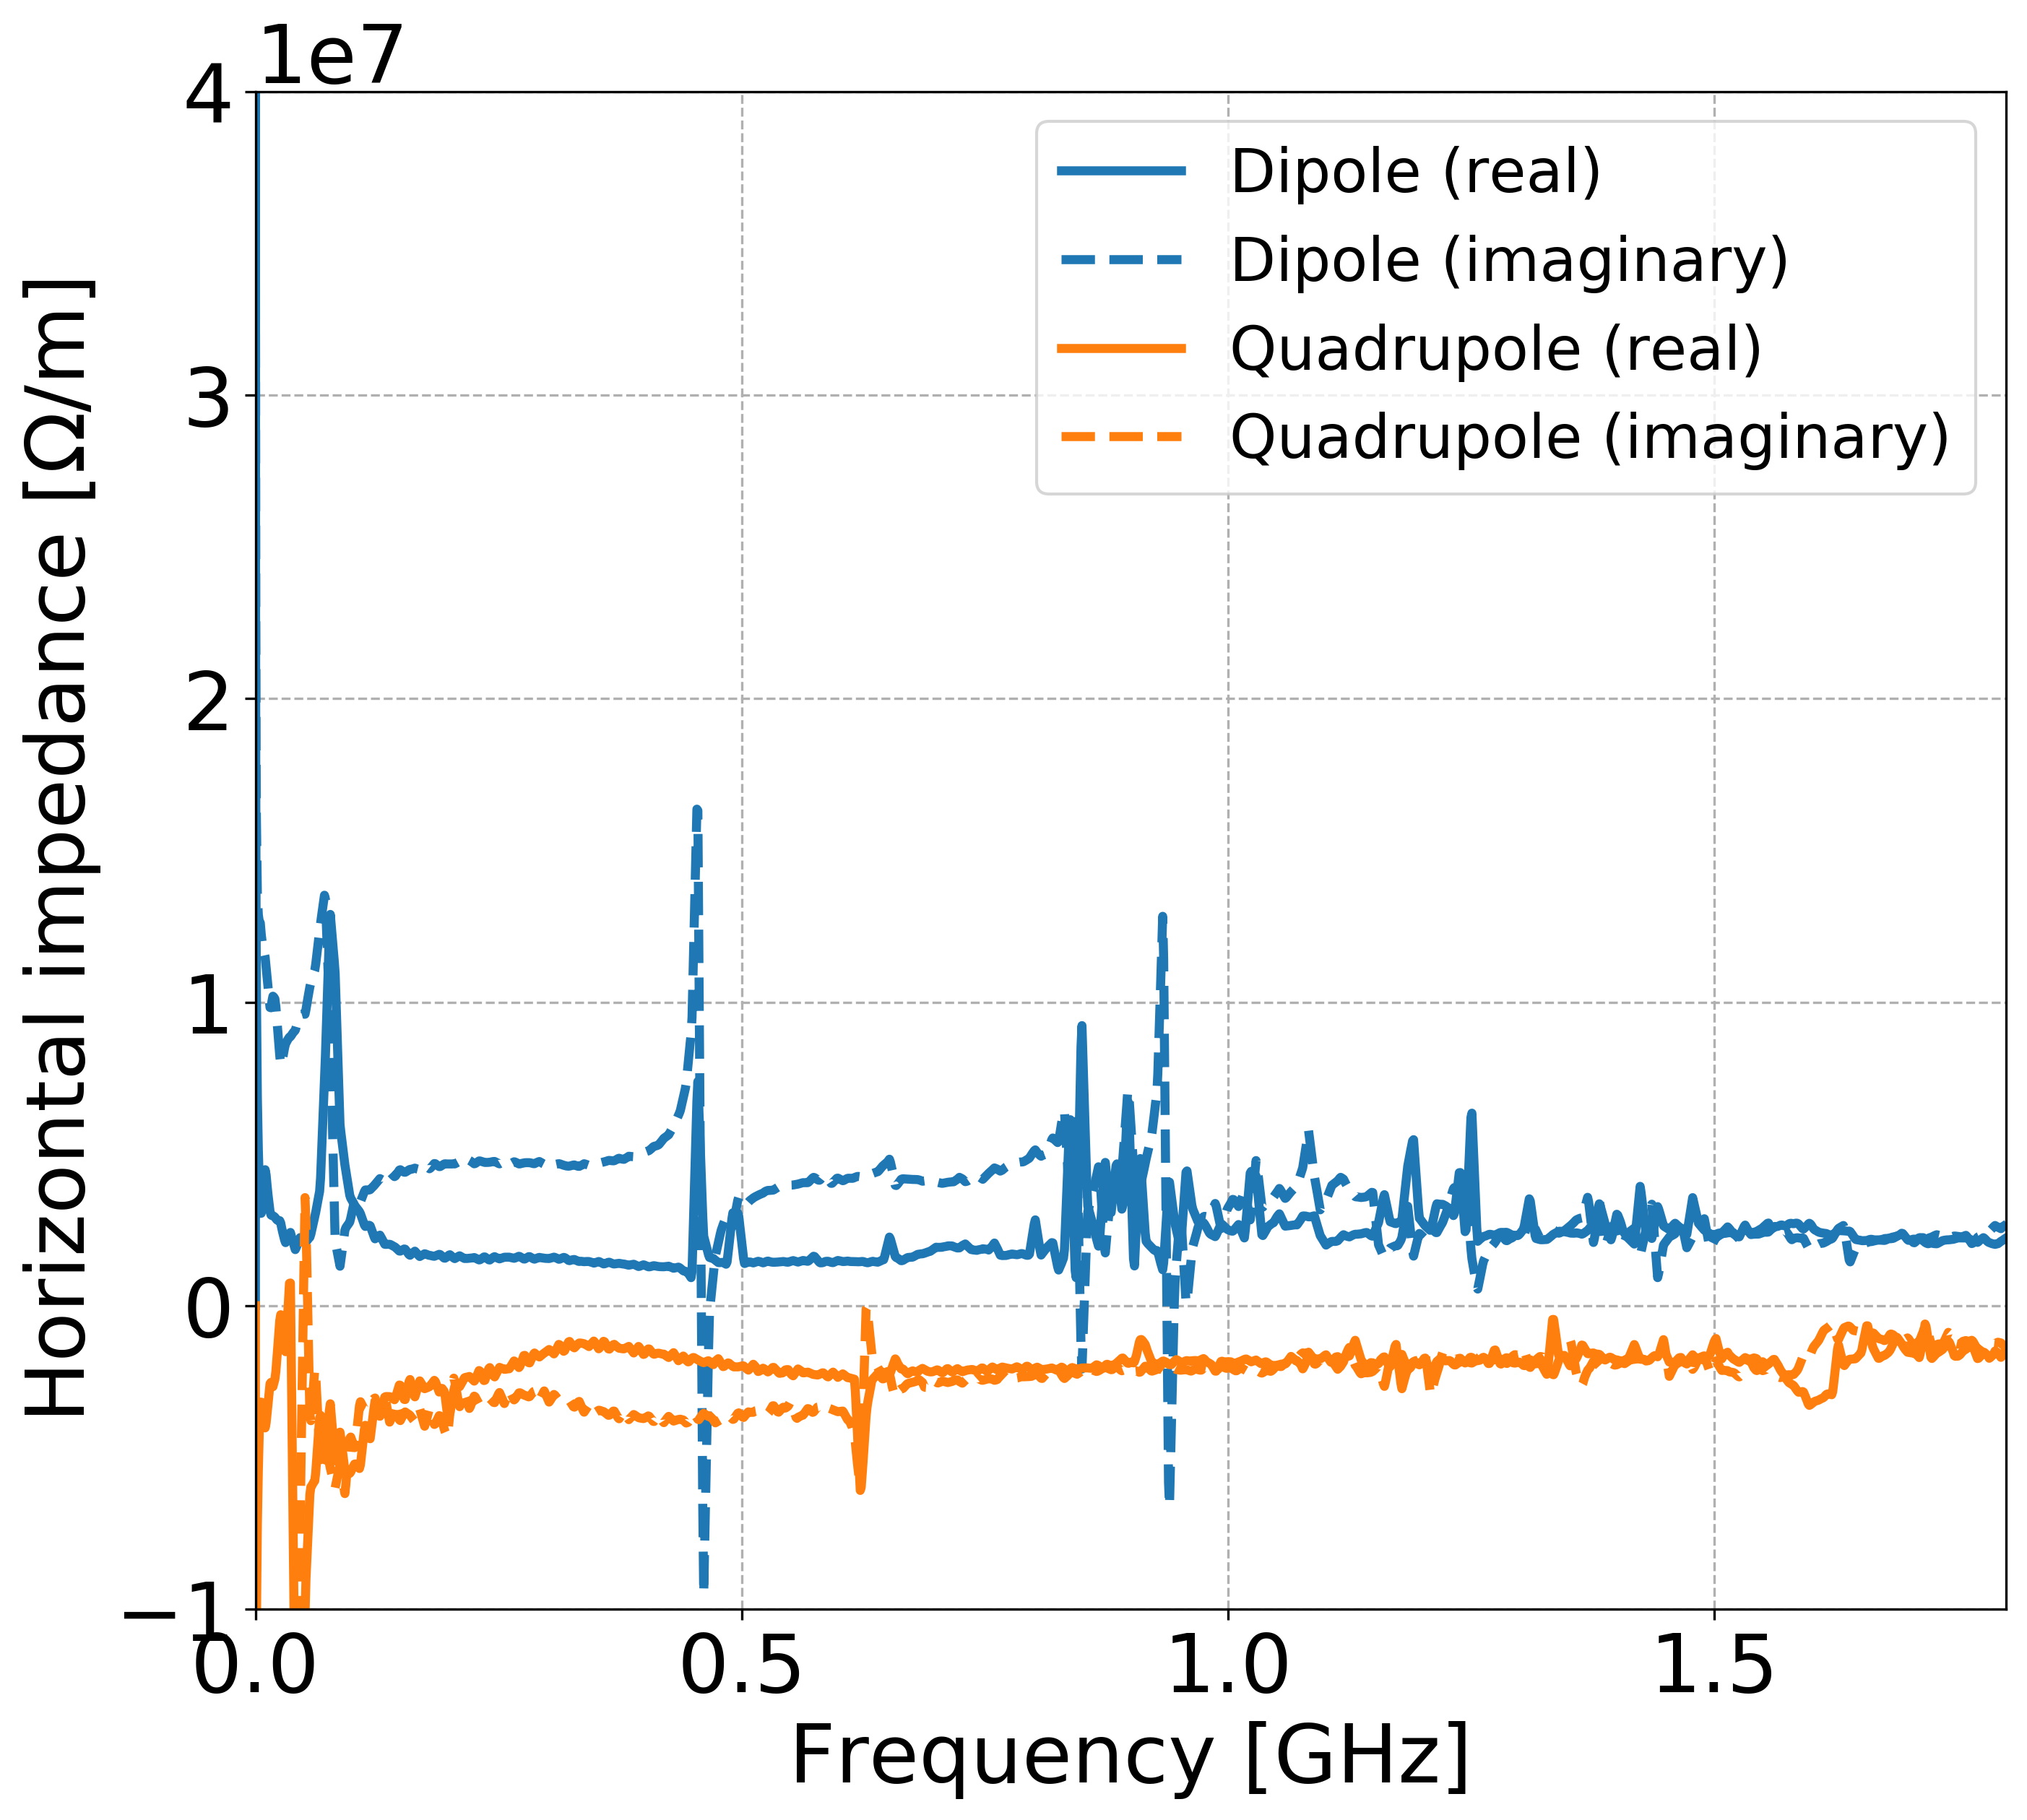
\includegraphics[width=1\textwidth]{images/Ch7/Q26_complete_SPS_model_impedance_H_plane.png}
        %\caption{$y=\sin(2 \pi f t),\ f=50$ Hz}
        %\label{fig:add_label_here}
    \end{subfigure}
    \hfill
    \begin{subfigure}[t]{0.45\textwidth}
        \centering
        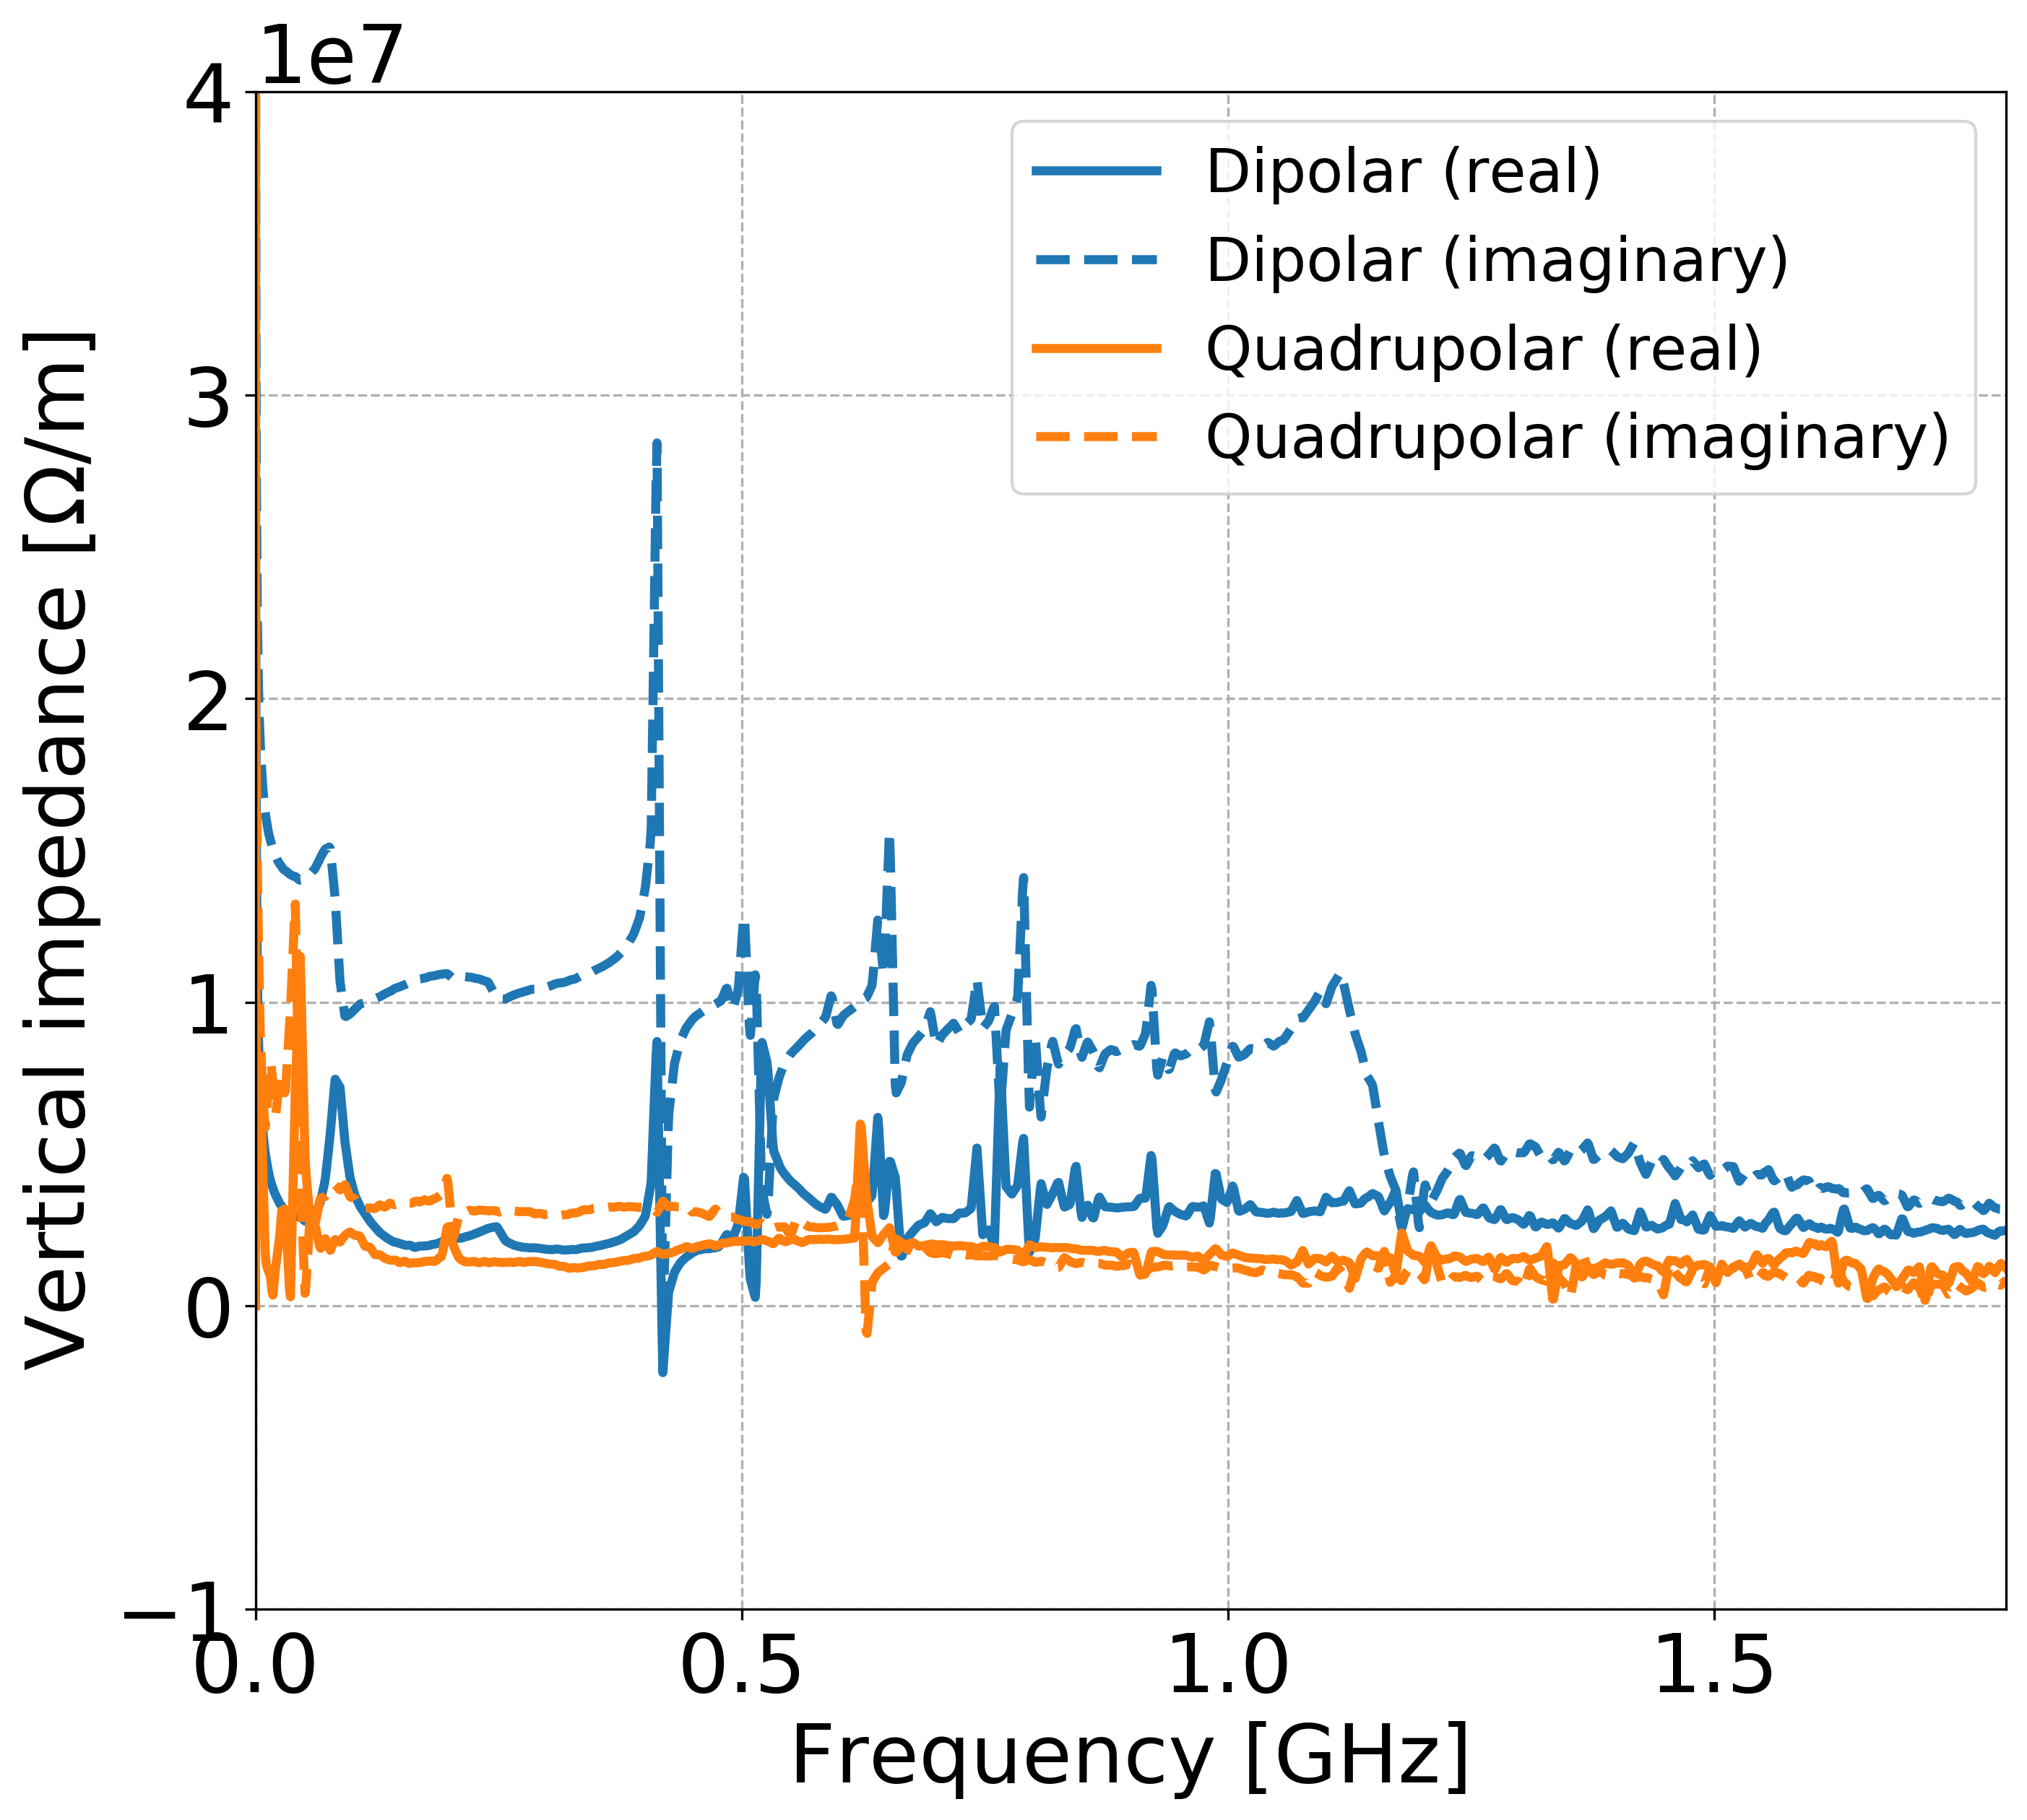
\includegraphics[width=1\textwidth]{images/Ch7/Q26_complete_SPS_model_impedance_V_plane.png}
        %\caption{Discrete Fourier transform}
        %\label{fig:add_label_here}
    \end{subfigure}
    \hfill
     \caption{Horizontal (left) and vertical (right) impedance model of the SPS. The model is available in the public gitlab repository of Ref.~\cite{sps_impedance_model_git}.} % bunch passage
     \label{fig:sps_impedance_model_H_V}
 \end{figure}

 The contributions from the wall, the kickers and the step transitions are visible at the low freqencies (up to $\sim$ 0.4\,GHz). The impedance of the RF cavities and the beam position monitors (BPMs) corresponds results to the peaks observed between $\sim$ 0.4-1\,GHz. 
%https://indico.cern.ch/event/299470/contributions/686509/attachments/564150/777102/LIUSPS_transverse_imp_5.pdf %For a clearer picture, it is worth mentioning that at low freqencies (up to $\sim$ 0.4\,GHz) the impedance is mainly from the wall the kickers and the step transitions. The peaks between $\sim$ 0.4-1\,GHz appear due to the RF cavities and the beam position monitors.
%https://indico.cern.ch/event/299470/contributions/686509/attachments/564150/777102/LIUSPS_transverse_imp_5.pdf


\normalsize{\textbf{Wake functions}}\\
As already discussed in Section~\ref{subsec:pyheadtail}, in order to include the impedance effects in PyHEADTAIL simulations the real-value wakefields in time domain are used. The wakefield kicks are computed as a convolution of the wake function with the moments of each particle. The total transverse dipolar (blue) and quadrupolar (orange) wake functions for both planes of the SPS can be found in the gitlab repository of Ref.~\cite{sps_impedance_model_git} and they are plotted in Fig~\ref{fig:sps_wakefunctions_model_H_V}.

% Plot figures: /eos/user/n/natriant/Project_thesis/plot_wakefields_impedances_SPS
 \begin{figure}[!ht]
    \centering
    \begin{subfigure}[t]{0.45\textwidth}
        \centering
        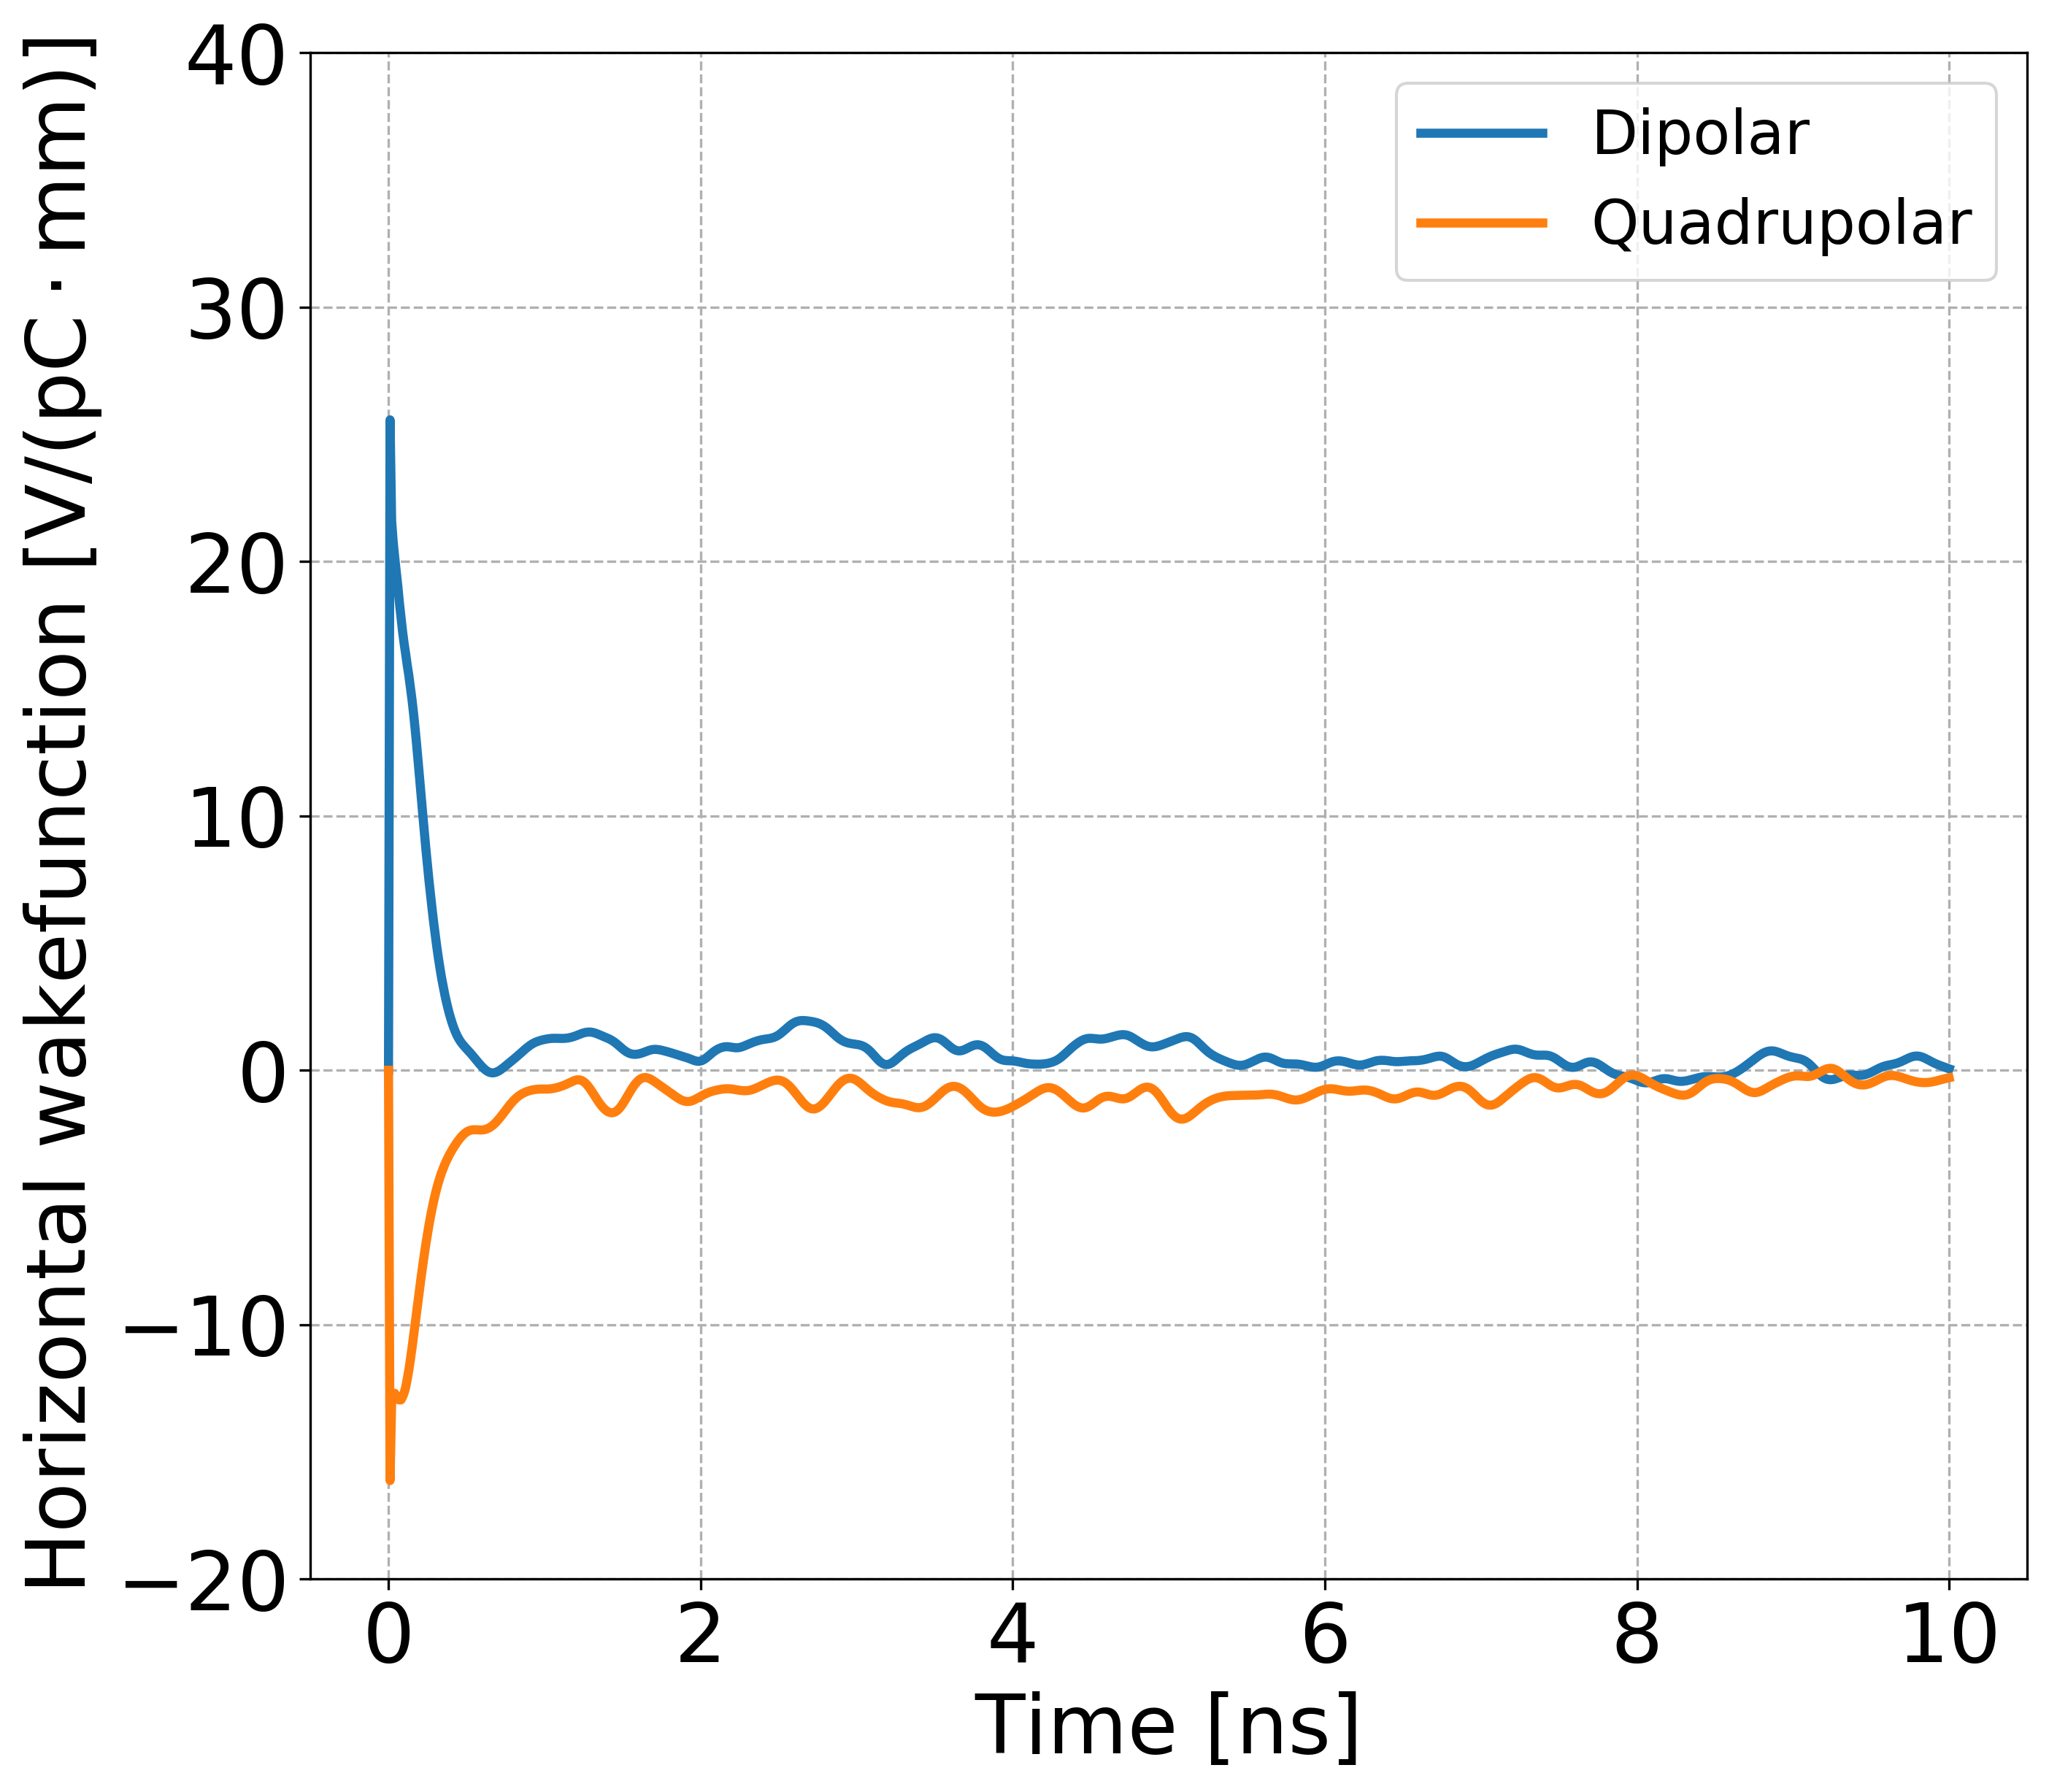
\includegraphics[width=1\textwidth]{images/Ch7/Q26_complete_SPS_model_wakefunctions_H_plane.png}
        %\caption{$y=\sin(2 \pi f t),\ f=50$ Hz}
        %\label{fig:add_label_here}
    \end{subfigure}
    \hfill
    \begin{subfigure}[t]{0.45\textwidth}
        \centering
        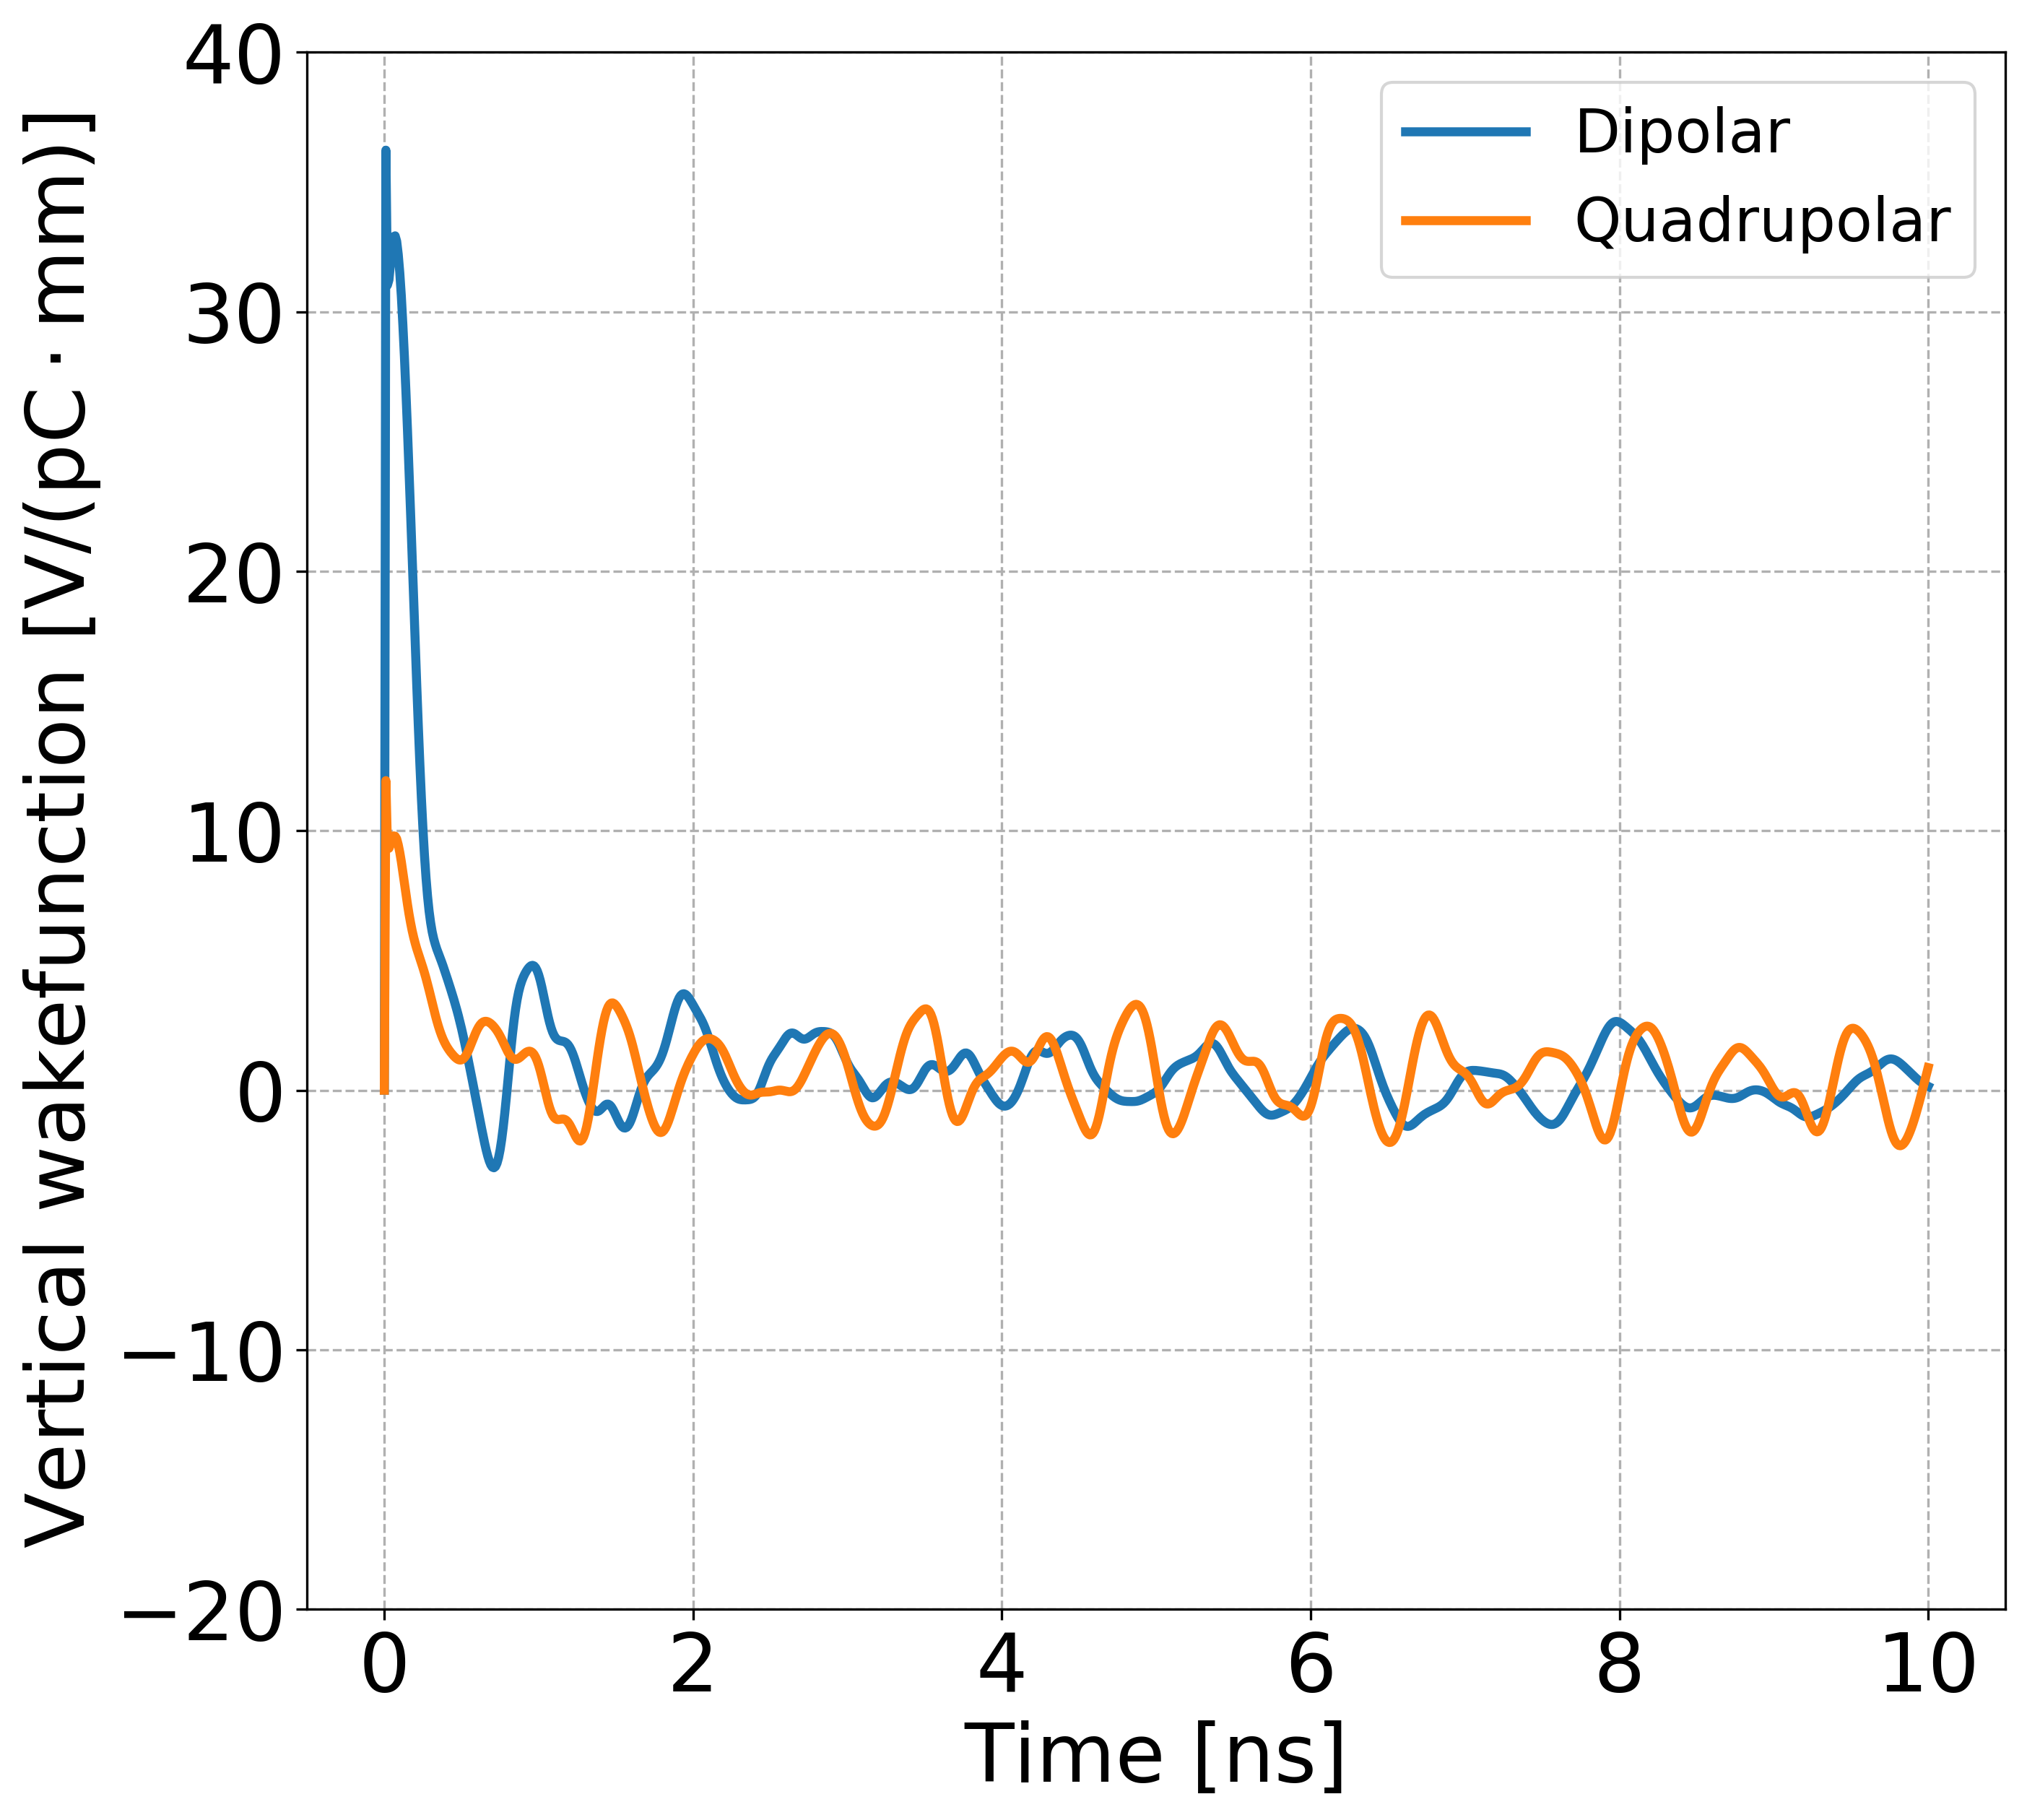
\includegraphics[width=1\textwidth]{images/Ch7/Q26_complete_SPS_model_wakefunctions_V_plane.png}
        %\caption{Discrete Fourier transform}
        %\label{fig:add_label_here}
    \end{subfigure}
    \hfill
     \caption{Horizontal (left) and vertical (right) wakefunctions of the SPS. The wake functions are available in the public gitlab repository of Ref.~\cite{sps_impedance_model_git}. For comparison the bunch length in the SPS CC experiments is $\sim$ 1.85\,ns (4$\mathrm{\sigma_t}$).} % bunch passage
     \label{fig:sps_wakefunctions_model_H_V}
 \end{figure}

 The constant terms, in both transverse planes, equal zero in the SPS impedance model. The reason behind this, is that firstly the constant term is usually coming from asymmetries in the various structures which are not significant, and secondly the constant term does not lead to instabilities or tune shift, so usually is not of big concern.

It should be highlighted that the impedance model is not obtained from a simple Fast Fourier Transform algorithm on the wakefunctions but rather with more complex procedures described in the references provided above. Last the imepdance model is used as an input in the Sacherer formula (Eq.~\eqref{eq:complext_tune_shift_modes_m}) for analytical estimations while the wake functions are used as an input in simulation codes such as PyHEADTAIL.


% slide 9 https://accelconf.web.cern.ch/ipac2019/talks/weypls1_talk.pdf

% Carlo Zaninni thesis: s, it is important to have an accurate description of the wake at a distance z significantly smaller than the RMS bunch-length, which means that the impedance calculation needs to be accurate up to very high frequency (depending on the accelerator we consider, from a few GHz to the range of THz). 

\subsection{Testing the implementation in PyHEADTAIL}\label{subsec:test_implementation_pyheatail}
As discussed in Section~\ref{subsec:wakefields} the imaginary part of the impedance leads to a coherent tune shift which depends on the bunch intensity. One of the most common ways to test the correct implementation of the impedance model in a tracking simulation code is to benchmark the simulated intensity-dependent coherent tune shift with the theoretically predicted behavior (using Eqs.~\eqref{eq:complext_tune_shift_modes_m} and ~\eqref{eq:real_tunu_mode_l}).

Typically, in tracking simulations, the coherent tune is obtained by applying a frequency analysis technique to the oscillations of the centroid of the particle distribution (the center of mass of the bunch). Here, the analysis is limited to the coherent mode $l=0$ as it can be obtained using a simple Fast Fourier Transform (FFT) algorithm~\cite{FFT_and_applications}. Higher modes (in absolute value, i.e. $l=\pm 1, \pm 2$ etc) can be obtained with more complex algorithms such as the oned provided from the SUSSIX code~\cite{Bartolini:702438} \footnote{The SUSSIX code is applied to the complex position in phase space, $u-i p_u$, while an FFT algorithm is applied only to the transverse position $u$, where $u=(x,y)$~\cite{Salvant:1274254}.}. Nevertheless, the study of mode $l=0$ is sufficient for the purpose of the studies presented here. For simplicity in the following the term "coherent tune" will refer to the coherent tune of mode $l=0$.

\textbf{Simulations setup}\\
The parameters used for setting up the linear transfer map, the longitudinal tracking, and the beam initialisation are shown in Table~\ref{tab:pyheadtail_simulation_parameters} and are the ones used in the SPS $\CC$ experiment of 2018. The ring is consisted of one segment, with one interaction point at which the beam interacts with the wakefields. At that location, the horizontal and vertical beta functions equal the corresponding average beta functions over the SPS machine (see Section~\ref{subsec:pyheadtail}). The latest transverse wakefield model (as of February 2019 in Ref.~\cite{sps_impedance_model_git}) of the SPS was used.

The bunch poulation of the different intensity values, was represented by $5 \times 10^5$ macroparticles and the number of slices of the longitudinal distribution was 500.

\begin{table}[!hbt]
	\begin{minipage}{\textwidth}
      \begin{centering}
   \caption{PyHEADTAIL simulation parameters used to study impedance induced effects for the SPS.}
	\begin{tabu} to \textwidth {X[c,m] X[0.5c,m] X[0.5c,m] X[0.01c,m]}
		&&& \\[-6mm]
		\toprule \toprule
		\multicolumn{2}{l}{\textbf{Parameter}} &
		\multicolumn{2}{c}{\textbf{Value}} \\
		\bottomrule
      \multicolumn{2}{l}{Beam energy, $\symE$} & \multicolumn{2}{c}{270\,GeV} \\
      \multicolumn{2}{l}{Machine circumference, $C_0$}  & \multicolumn{2}{c}{6911.5623\,kHz} \\
      \multicolumn{2}{l}{Horizontal / Vertical betatron tune, $\Qx$ / $\Qy$}  & \multicolumn{2}{c}{26.13 / 26.18} \\
      \multicolumn{2}{l}{Synchrotron tune, $\Qs$}  & \multicolumn{2}{c}{0.0051}\\
      \multicolumn{2}{l}{Momentum compaction factor, $\alpha_p$}  & \multicolumn{2}{c}{1.9 $\times 10^{-3}$}\\
      \multicolumn{2}{l}{Number of bunches}  & \multicolumn{2}{c}{1} \\
      \multicolumn{2}{l}{Rms bunch length, 4$\sigmat$}  & \multicolumn{2}{c}{1.7\,ns}\\
      \multicolumn{2}{l}{Horizontal / Vertical normalised emittance, $\epsilon_x$ / $\epsilon_y$}  & \multicolumn{2}{c}{2\,$\mathrm{\mu m}$ / 2\,$\mathrm{\mu m}$}\\
      \multicolumn{2}{l}{Average horizontal / vertical beta function, $\langle \beta_x \rangle / \langle \beta_y \rangle$}  & \multicolumn{2}{c}{42.0941\,m / 42.0137\,m $^\ast$ } \\
      \bottomrule
      \multicolumn{2}{l}{Number of macroparticles, $N_\mathrm{mp}$}  & \multicolumn{2}{c}{$5 \times 10^5$} \\
      \multicolumn{2}{l}{Number of longitudinal slices, $N_\mathrm{slices}$}  & \multicolumn{2}{c}{500} \\
      \bottomrule
	\end{tabu}
   \label{tab:pyheadtail_simulation_parameters}
   \end{centering}\footnotesize{$^\ast$ Model values for the Q26 optics.}
   \end{minipage}
\end{table}

For all the PyHEADTAIL simulation studies presented in this thesis, the Twiss parameter $\alpha_u(s)$ and the dispersion function $D_u(s)$ equal zero. This is a valid assumption for the studies as these parameters have no direct impact on the effects under investigation.

To facilitate the observation of the coherent tune, the bunch was intialised with a static offset of 0.15$\sigma_{x,y}$ in both transverse planes\footnote{The rms transverse beam size at the only interaction point along the ring i.e. at the location where the beam interacts with the wakefields.}, such as it performs dipole oscillations around the machine. Then, it was tracked for 600 turns and the coherent tune was computed using a NAFF algorithm~\cite{LASKAR1990266, Kostoglou:2289645}, which provides a refined FFT analysis, and its python implementation, NAFFlib, can be found in the corresponding package in Ref.~\cite{nafflib_repository}, on the turn-by-turn centroid motion. The coherent tune shift was computed by subtracting the obtained tune value from the unperturbed coherent tune (in the absence of impedance) which equals the $Q_{u0}$ value.


Finally, the dependence of the coherent tune on the intensity value was studied in the absence of other detuning effects (such as chromaticity or detuning with transverse amplitude, even though they mainly introduce incoherent tune shifts). % Do they also introduce some small coherent tune?

The simulation was repeated for a range of bunch intensities, $N_b$, equally-spaced from 0 to $5 \times 10^{10}$ protons per bunch. This range was chosen to be in the vicinity of the bunch intensity of the $\CC$ experiments of 2018, where $N_b$ was $3\times 10^{10}$ protons per bunch. $N_b=0$ is not a realistic value. However, it is used here as the reference point for which the coherent betatron tune equals zero. The simulation results are plotted against the theoretically expected tune shifts in Fig.~\ref{fig:sps_coherent_DQ_vs_intensity_original_complete_model}.

The theoretically expected values are computed from Eqs.~\eqref{eq:complext_tune_shift_modes_m} and ~\eqref{eq:real_tunu_mode_l} for $l=0$ and using only the imaginary part of the imepdance. Given that $\Gamma(1/2)=\sqrt{\pi}$ and $Q_u = \omega_{u0}/\omega_\mathrm{rev}$ equation Eq.~\eqref{eq:complext_tune_shift_modes_m} becomes:
\begin{equation}\label{eq:real_tune_shfit_for_coherent_mode}
    \Delta \Omega_u^{(0)} =  \Omega_{u0}^{(0)} - \omega_{u0} = \frac{\sqrt{\pi}}{4 \pi}\frac{N_b r_0 c^2}{\gamma_0 \frac{2\pi}{\omega_\mathrm{rev}}\omega_u \sigma_z} Z_\mathrm{eff, im} = \frac{N_b r_0 c^2}{8 \pi^{3/2} \gamma_0 Q_u \sigma z}Z_\mathrm{eff, im}
\end{equation}
All the parameters inserted in Eq.~\eqref{eq:real_tune_shfit_for_coherent_mode} should be converted in CGS (centimetre–gram–second) units.

Then the coherent betatron tune shift is computed by inserting the result of Eq.~\eqref{eq:real_tune_shfit_for_coherent_mode} in Eq.~\eqref{eq:real_tunu_mode_l} such as 
\begin{equation}
    \Delta Q_u = \frac{\Delta \Omega_u^{(0)}}{\omega_\mathrm{rev}}.
\end{equation}


 % pyheadtail_data/final_for_thesis/2018_conditions/study_0_DQ_vs_intensity/
\begin{figure}[!ht]
    \centering
    \begin{subfigure}[t]{0.45\textwidth}
        \centering
        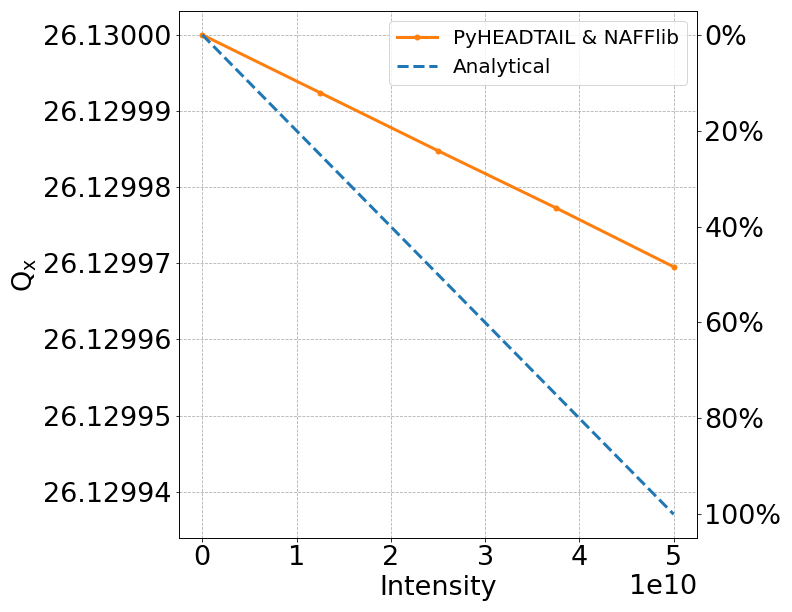
\includegraphics[width=1\textwidth]{images/Ch7/Qx_vs_intensity_complete_impedance_sps_q26model_MD2018_parameters.png}
        %\caption{$y=\sin(2 \pi f t),\ f=50$ Hz}
        %\label{fig:add_label_here}
    \end{subfigure}
    \hfill
    \begin{subfigure}[t]{0.45\textwidth}
        \centering
        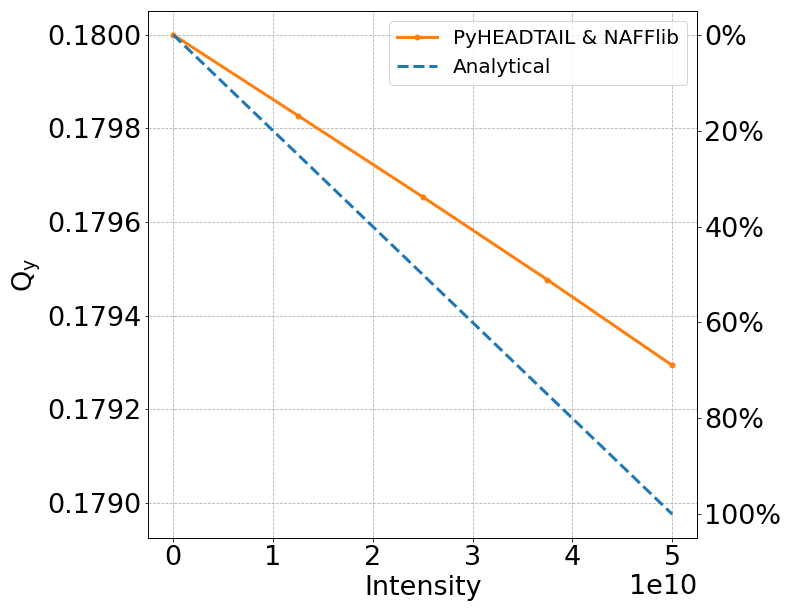
\includegraphics[width=1\textwidth]{images/Ch7/Qy_vs_intensity_complete_impedance_sps_q26model_MD2018_parameters.png}
        %\caption{Discrete Fourier transform}
        %\label{fig:add_label_here}
    \end{subfigure}
    \hfill
     \caption{Horizontal (left) and vertical (right) coherent tunes as a function of intensity in the presence of the beam coupling SPS imepdance obtained using analytical formula (blue dashed line) and PyHEADTAIL tracking simulations (orange line). The impedance model and the wake functions used are available in the public gitlab repository of Ref.~\cite{sps_impedance_model_git}.} % bunch passage
     \label{fig:sps_coherent_DQ_vs_intensity_original_complete_model}
 \end{figure}

 Figure~\ref{fig:sps_coherent_DQ_vs_intensity_original_complete_model} shows that the coherent tune shift from the analytical model does not agree with simulation results. In particular the wakefields implementation in the PyHEADTAIL results just to $\sim 50 \%$ and $\sim 70 \%$ of the total coherent tune shift estimated using the analytical formula of Sacherer with the impedance model. This discrepancy hadn't been observed before as this study has not been conducted for such low intensities (the usual intensity range for this type of study is in the order of $10^{11}$ protons per bunch ~\cite{Beck:2683038}) and short bunches. %p.101
 The analytical predictions from Sacherer formula have been repeatedly successfully benchmarked against beam measurements~\cite{Bartosik:1742183, sps_impedance_measurements_vs_model} which indicates that there is an issue with the model of the wakes or with their implementation in the simualtion. Given the fact that the studies with $\CC$s are quite sensitive on the coherent tune shift with intensity from the coupling impedance (this will be discussed in the following paragraphs of this chapter) it is crucial to identify the reason for the observed discrepancy and resolve it.

 After several studies and discussions with the experts on the topic \footnote{In particular with Carlo Zannini, carlo.zannini@cern.ch.} it was identified that the components of the resistive wall and the step transitions needed to be re-computed to provide higher accuracy at the lower frequencies. The details of this work are not discussed here as they are out of the scope of this thesis and they were not performed by the author. The re-computed wake functions along with the rest of the components of the original model can be found in the gihub repository of Ref.~\cite{updated_sps_wakfields_model} and it will be reffered to as the "updated wakefields" model.

 The coherent betatron tune as a function of intensity obtained using PyHEADTAIL and the updated wakefields model is plotted in Fig.~\ref{fig:sps_coherent_DQ_vs_intensity_updated_model} against the analytical predictions from Sacherer formula. In the both transverse planes, the results from the simulations and the theory are in very good agreement ($\leq 5\%$) which is within the uncertainty that one can expect from the model implementation. 

 % pyheadtail_data/final_for_thesis/2018_conditions/study_0_DQ_vs_intensity/
\begin{figure}[!ht]
    \centering
    \begin{subfigure}[t]{0.45\textwidth}
        \centering
        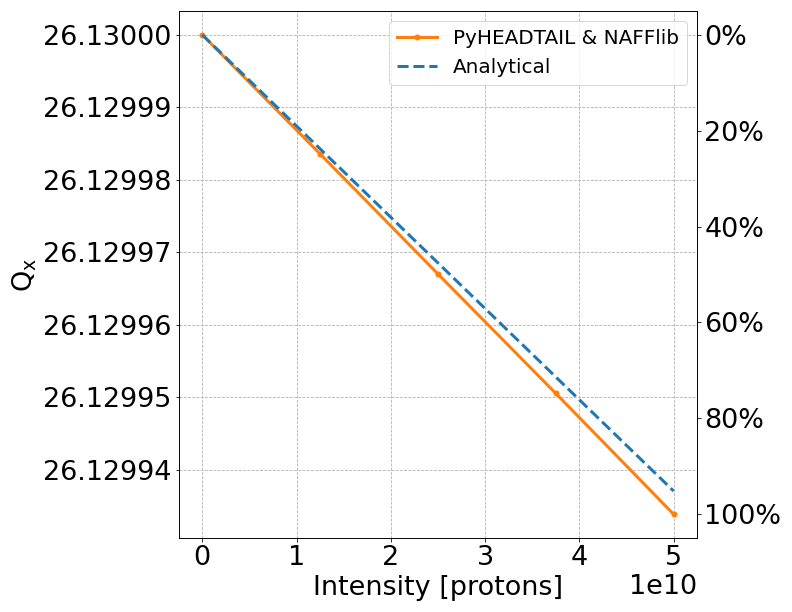
\includegraphics[width=1\textwidth]{images/Ch7/Qx_vs_intensity_complete_impedance_sps_q26model_updated_MD2018_parameters_integer.png}
        %\caption{$y=\sin(2 \pi f t),\ f=50$ Hz}
        %\label{fig:add_label_here}
    \end{subfigure}
    \hfill
    \begin{subfigure}[t]{0.45\textwidth}
        \centering
        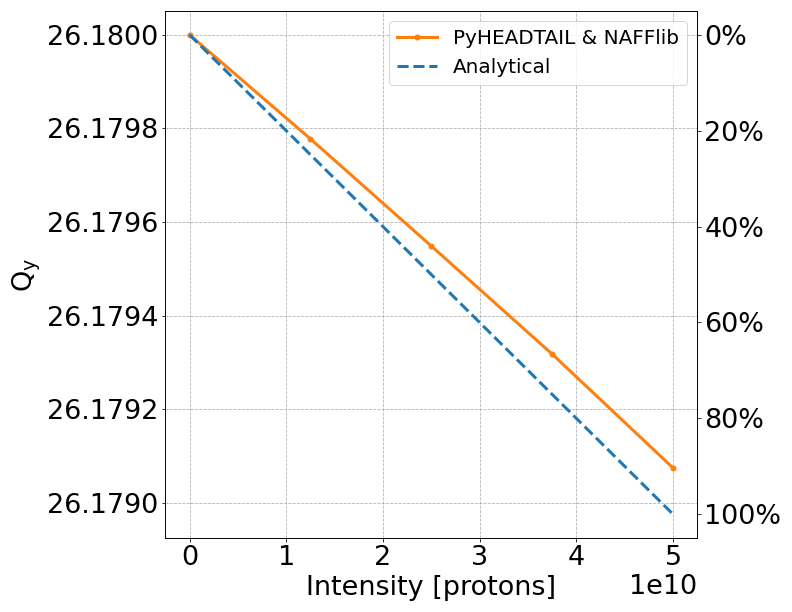
\includegraphics[width=1\textwidth]{images/Ch7/Qy_vs_intensity_complete_impedance_sps_q26model_updated_MD2018_parameters_integer.png}
        %\caption{Discrete Fourier transform}
        %\label{fig:add_label_here}
    \end{subfigure}
    \hfill
     \caption{Horizontal (left) and vertical (right) coherent tunes as a function of intensity in the presence of the beam coupling SPS imepdance obtained using analytical formula (blue dashed line) and PyHEADTAIL tracking simulations (orange line). The impedance model and the wake functions ("updated wakefields" model) used are available in the public repositories of Ref.~\cite{sps_impedance_model_git} and Ref.~\cite{updated_sps_wakfields_model} respectively.} % bunch passage
     \label{fig:sps_coherent_DQ_vs_intensity_updated_model}
 \end{figure}

 The above figure demonstrates that the updated wakefields model is reliable and it confirms that its implementation in PyHEADTAIL is correct. Therefore it will be used to study the interplay of the $\CC$ noise induced emittance growth with impedance induced effects. These studies are presented in the following chapter.

 %The above figure confirms the correct implementation of the updated wakefields model in PyHEADTAIL and therefore it will be used to study the interplay of the $\CC$ noise induced emittance growth with impedance induced effects. These studies are presented in the following chapter.

\section{Emittance growth simulations setup}\label{sec:setup_simulations_emit_growth}
The simualtions that were performed to investigate the impact of the beam coupling impedance on the $\CC$ RF noise-induced emittance growth were performed following the procedure and using the parameters that are described below. Any change in the choice of parameters, e.g. for some of the parametric studies, will be mentioned in the corresponding paragraph.

The parameters used for setting up the linear transfer map, the longitudinal tracking, and the beam initialisation are shown in Table~\ref{tab:pyheadtail_simulation_parameters} and are the ones used in the SPS $\CC$ experiment of 2018. The ring is consisted of two segments with two interaction points. In the first one $\CC$ noise-like kicks are applied on the beam particles while in the second one the the beam interacts with the wakefields as discussed in the previous section. The updated wakefields model Ref.~\cite{updated_sps_wakfields_model} of the SPS was used.

At the location of the $\CC$ RF noise kick the horizontal and vertical beta functions equals the values at the location of the $\CC2$ which was used in the experiments of 2018. At the location, where the wakefield kicks are applied the transverse beta functions equal the corresponding average beta functions over the SPS machine (see Section~\ref{subsec:pyheadtail}). 

As already discussed in the previous section, the simualtions are performed for the Twiss parameter $\alpha_u(s)$ and the dispersion function $D_u(s)$ equal zero. This is a valid assumption for the studies as these parameters have no direct impact on the effects under investigation.

The emittance growth studies were performed for intensity of $3 \times 10^{10}$ protons per bunch in accordance with the 2018 experiments. The bunch population was represented by $5 \times 10^{5}$ macroparticles and the number of longitudinal slices was 500. The emittance growth was also simulated without including the wakefields. For the latter case the bunch population was represented by $10^{5}$ particles and no longitudinal slicing was applied. The studies were performed using an initial Gaussian bunch distribution in the six-dimensional phase space. This is a good approximation for the bunches used in the experimental studies of 2018. 

At the location of the $\CC$ RF noise kick, the angle, $y^\prime$, of each particle within the bunch is updated every turn according to the kicks of Eqs.~\eqref{eq:amplitude_noise_kick} and~\eqref{eq:phase_noise_kick} for amplitude and phase noise kick respectively. The scaling factor, $A$ equals $10^{-8}$ excpet if it is stated otherwise. This noise level, which corresponds to power spectal density of $1.68 \cdot 10^{-10} \mathrm{rad^2/Hz}$ or $\mathrm{1/Hz}$ for phase and amplitude noise respectively is much stronger than the ones of the actual $\CC$ RF system and was chosen such as it results in a reasonable growth in the simulation time of $10^5$ turns (it corresponds to $\sim$2.5 seconds in the SPS). The emittance growth over the course of the simulation is comparable to that during a coast though. This approach is valid due to the linear growth of emittance with time and the linear scaling with the noise level~\cite{PhysRevSTAB.18.101001}. The parameters used for the implementation of the $\CC$ RF noise kick in the simulations are shown in Table~\ref{tab:CC_pyheadtail_simulation_parameters}.

\begin{table}[!hbt]
	\begin{minipage}{\textwidth}
      \begin{centering}
   \caption{PyHEADTAIL simulation parameters used for the implementation of the CC RF noise kicks for the emittance growth studies. This table is complementary of Table~\ref{tab:CC_pyheadtail_simulation_parameters}.}
	\begin{tabu} to \textwidth {X[c,m] X[0.5c,m] X[0.5c,m] X[0.01c,m]}
		&&& \\[-6mm]
		\toprule \toprule
		\multicolumn{2}{l}{\textbf{Parameter}} &
		\multicolumn{2}{c}{\textbf{Value}} \\
		\bottomrule
      \multicolumn{2}{l}{Horizontal / vertical beta function, $\beta_{x, \mathrm{CC}} / \beta_{y, \mathrm{CC}}$}  & \multicolumn{2}{c}{30.31\,m / 73.82\,m } \\
      \multicolumn{2}{l}{CC frequency, $f_\mathrm{CC}$}  & \multicolumn{2}{c}{400.78\,MHz} \\
      \multicolumn{2}{l}{Scaling factor for amplitude and phase noise, $A$}  & \multicolumn{2}{c}{$10^{-8}$} \\
      \bottomrule
	\end{tabu}
   \label{tab:CC_pyheadtail_simulation_parameters}
   \end{centering}
   \end{minipage}
\end{table}

Last, the emittance growth simulation studies were performed for non-zero linear chromaticity and for non-zero detuning with the transverse amplitude. Both effects were introduced as changes in the phase advance of the individual particles according to Eq.~\eqref{eq:change_phase_advance_detunign}. The value of the linear chromaticity, $Q^{\prime}_{x,y}=0.5$ for most of the studies according to the experimental conditions of 2018. Higher order chromaticities were considered negligible. The values of the detuning coefficients will be given in the following sections.


In the following sections, the emittance growth rates will be expressed in nm/s due to the simulation time scale and will be referred to the growth of the normalised emittance values to be in agreement with the analyisis of the measured data in Chapter~\ref{Ch:2018_analyisis}.

\section{First observations of emittance growth suppression by the impedance}\label{sec:first_obs_suppression}

The first emittance growth simulations were performed for the beam and machine conditions of the 2018 experiments. The parameters are listed in Tables~\ref{tab:pyheadtail_simulation_parameters} and~\ref{tab:CC_pyheadtail_simulation_parameters} and the detailed procedure is described in Section~\ref{sec:setup_simulations_emit_growth}. To give an overview, the study was conducted for a single proton bunch, energy of 270\,GeV, bunch intensity of $3 \times 10^{10}$ protons, rms bunch length $4 \sigma_t = 1.7$\,ns and linear chromaticity of 0.5 in both transverse planes. 

$\CC$ phase noise was applied as it was the dominant type in the 2018 experiment, with power spectral density of $1.68 \times 10^{-10} \mathrm{rad^2/Hz}$ which corresponds to $A=10^{-8}$ for the scaling factor of Eq.~\eqref{eq:phase_noise_kick}. For this noise power a growth rate of about 25\,nm/s is expected (exciting the first betatron sidebands at $\pm$7.8~\,kHz, see further discussion in Section~\ref{subsec:CC_emit_growth_theoretical_formulas}). 

The geometric emittance value was computed every 100 turns (for computational efficiency) using the statistical definition which can be found in Eq.~\eqref{eq:geometric_emittance_v2}. The emittance growth rate was computed by performing a linear fit to the normalised (using Eq.~\eqref{eq:normalised_emittance}) emittance values over the simualtion turns ($N_\mathrm{turns}=10^5$). Twenty simulation runs were conducted, to reduce the uncertainty of the results. The initial bunch distribution and the sequence of the uncorrelated noise kicks were regenerated randomly for every run. The mean and the standard deviation (including the uncertainty on the slope of the fit) were computed over all the trials.  

As mentioned in Chapter~\ref{Ch:2018_analyisis} the Landau octupoles were switched off during the 2018 $\CC$ experiment. Nevetherless, a residual non-linearity was present in the machine mainly due to multipole components in the dipole magnets~\cite{Carlà:2664976, Alekou:2640326}. As the machine non-linearities were not explicitly characterised during the experiment, the dependence on the octupole-like amplitude dependent tune spread was studied. Instead of using an actual octupolar (non-linear) element which would result to resonance excitation\footnote{In the real SPS machine the Landau octupoles are installed in families of focusing and defocusing in order to avoid the excitation of resonances.}, the amplitude dependent tune shift was introduced as changes to the phase advance of the particles depending on their individual action as discussed in Eq.~\eqref{eq:change_phase_advance_detunign}. More specifically, the dependence on the detuning coefficient in the vertical plane, $\alpha_{yy}$, was studied. In particular $\alpha_{yy}$ ranges from $-$20000 to 20000\,1/m . For the studies presented here and in the following sections of this chapter, the horizontal detuning coefficient and the cross-term were left at zero for simplicity, i.e.~$\alpha_{xx} = \alpha_{xy} = 0$. % for better control over the simulations. This choice is also based on the fact that their value doesn't affect the results.
The sensitivity on the cross-term is discussed in the Chapter~\ref{Ch:experimental_CC_2022}, again for $\alpha_{xy} = 0$ as the horizontal coefficient does not affect the vertical emittance growth since there is no coupling between the two transverse planes.

The simulations were performed with and without the SPS impedance model to study its impact on the emittance growth induced by CC noise. Figure~\ref{fig:MD_2018_impedance_simulations} shows the dependence of the growth rates on the amplitude detuning coefficient, $\alpha_{yy}$. The secondary horizontal axis shows the resulting rms tune spread computed using Eq.~\eqref{eq:rms_amplitute_detuning_3}. Incoherent tune shift from other sources, than the detuning with transverse amplitude are not included. In particular, the effect of chromaticity is not taken into account in the computation of the tune spread as it varies periodically with the synchrotron period \textcolor{red}{(does it cancel out?)} and the incoherent tune shift from the impedance is considered negligible. 

\begin{figure}[!h] % at the directory of ipac22
    \centering         
    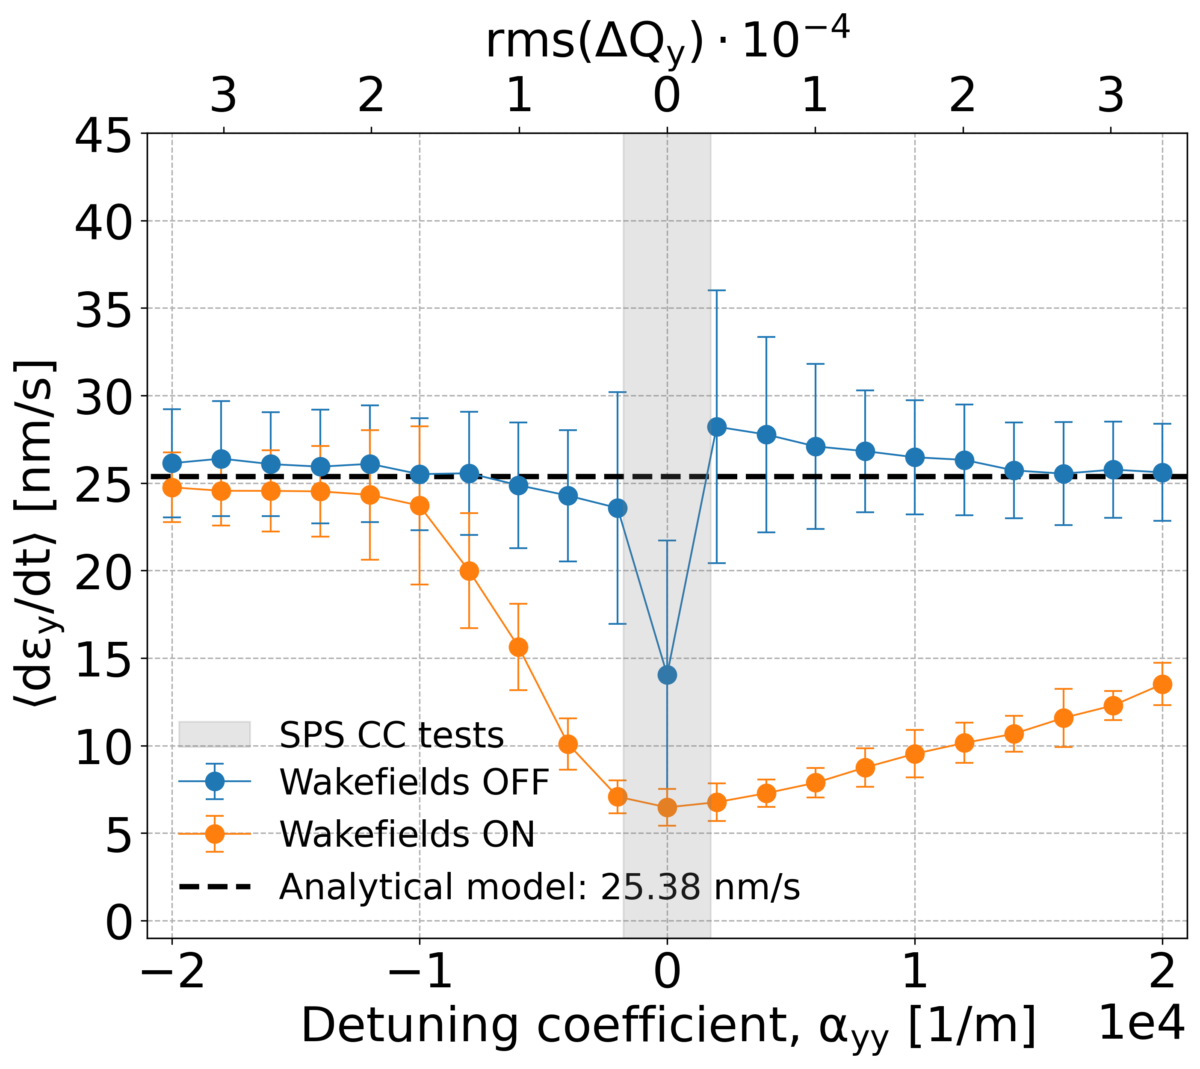
\includegraphics[width=0.85\textwidth]{images/Ch7/deyRates_final_2018_PN_sps_270GeV_PN1e-8_400MHz_y-plane_QpxQpy5e-1_6D_Nb5e5_intensity3e10_ayyScan_wakesON_vs_OFF_vs_TuneSpreadvsExpectedSPS.png}
        \caption{Transverse emittance growth driven by CC RF phase noise without (blue) and with (orange) the impedance effects.}
        \label{fig:MD_2018_impedance_simulations}
 \end{figure}

It can be seen that when the wakefield kicks are not applied on the beam the emittance growth rate agrees very well with the value predicted by Eq.~\eqref{eq:dey_pn} and (within the reproducibility of the simulation) is independent of the tune spread value. It should be noted that the theoretical model is not valid for zero tune spread, and that the observed emittance growth rate for $\alpha_{yy} = 0$ is a result of the geometric distortion of the beam caused by the $\CC$ kick.

Figure~\ref{fig:MD_2018_impedance_simulations} also shows a clear suppression of the transverse emittance growth when the wakefield kicks are included. The suppression depends on the tune spread and is asymmetric for positive and negative values of the detuning coefficient. Over a realistic range of tune spread values (estimated with MAD-X~\cite{madx} including the non-linearities of SPS~\cite{Carlà:2664976, Alekou:2640326} and $Q^\prime_{x,y}$ = 0.5, and shown by the grey shaded area in Fig.~\ref{fig:MD_2018_impedance_simulations}) the suppression reaches up to a factor 4-5. This suppression is very close to that observed in the experiments and suggests that the impedance effects might explain the discrepancy between the measured and theoretically estimated emittance growth rates.

To sum up, PyHEADTAIL simulations showed for the first time that the transverse beam impedance (which is not included in the theory of P.~Baudrenghien and T.~Mastoridis~\cite{PhysRevSTAB.18.101001}) has a significant impact on the emittance growth driven by $\CC$ RF noise. The effect of the suppression of noise-induced emittance growth from the impedance has not been observed before. 
To characterise this effect and to be able to understand the mechanism behind it, a series of exploratory studies were conducted and are discussed in the following section. 


\section{Characterisation of the emittance growth suppression by the impedance}\label{sec:emittance_growth_exploratory_studies}

This section, discusses the results of the exploratory simulation studies which investigate the suppression of the $\CC$ RF noise-induced emittance growth be the transverse beam coupling impedance. The goal is to characterise the effect and understand the mechanism behind it. First, the impact of the imepdance is studied in the presence of amplitude noise and in the presence of a noise kick (both in amplitude and phase) from a $\CC$ with the same frequency as the main RF system of the machine (HL-LHC scenario). Then, the effect of the impedance in the presence of a pure dipolar noise kick was simulated followed by a sensitivity study on the impact of the linear chromaticity. Finally, the impact of the dipolar and quadrupolar wakefields was disentangled. 

The simulations were conducted following the same pattern as the case discussed in the previous section. Nevertheless, the main relevant parameters for each case will also be listed in the corresponding section.

\subsection{Amplitude noise}\label{subsec:amplitude_noise}
The simulations discussed here were performed with and without the SPS imepdance model in the presence of $\CC$ RF amplitude noise, with power spectral density of $1.68 \times 10^{-10}$ 1/Hz which corresponds to $A=10^{-8}$ for the scaling factor in Eq.~\eqref{eq:amplitude_noise_kick}. The amplitude of the amplitude noise kicks equals the one of the phase noise kicks used in the previous section. The results are shown in Fig.~\ref{fig:study_1_2018_paramters_AN}.

\begin{figure}[!h] % at the directory of ipac22
    \centering         
    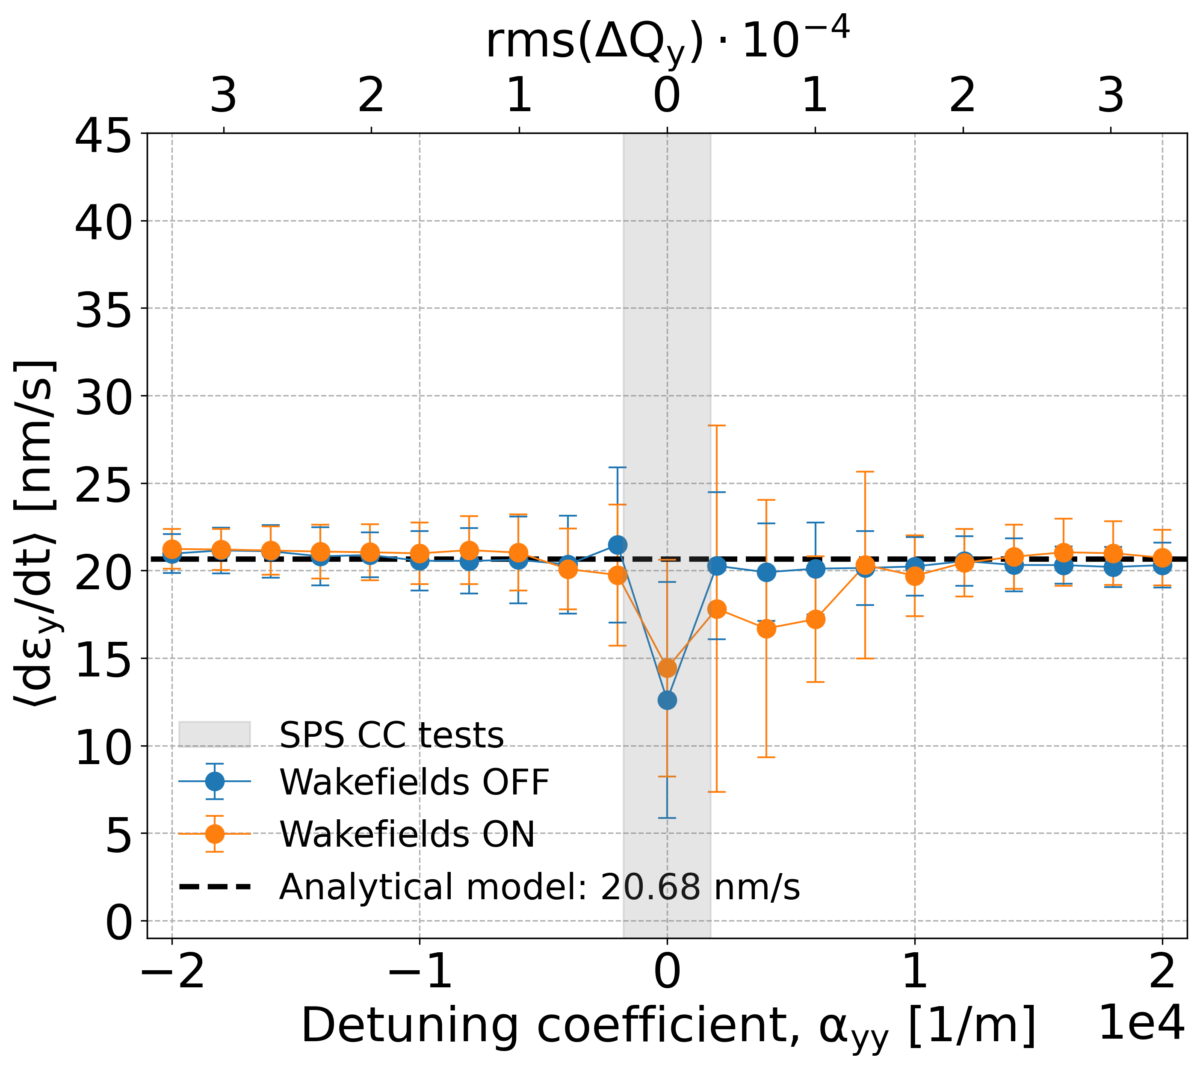
\includegraphics[width=0.85\textwidth]{images/Ch7/deyRates_final_2018_AN_sps_270GeV_AN1e-8_400MHz_y-plane_QpxQpy5e-1_6D_Nb5e5_intensity3e10_ayyScan_wakesON_vs_OFF_vs_TuneSpreadvsExpectedSPS.png}
        \caption{Transverse emittance growth driven by CC RF amplitude noise without (blue) and with (orange) the impedance effects.}
        \label{fig:study_1_2018_paramters_AN}
 \end{figure}

 It can be seen that the emittance growth rate agrees very well with the value predicted by Eq.~\eqref{eq:dey_an} and (within the reproducibility of the simulation) is independent of the tune spread value both when the wakefields are included and when they are not. In other words, the simulations demonstrate that the emittance growth driven by $\CC$ RF amplitude noise (which is associated with the headtail mode 1) is not suppressed by impedance induced effects. As the phase noise kick is similar to a dipolar noise kick (headtail mode 0) but with a high order distortion it seems that the suppression form the impedance is related to the dipole motion.


 \subsection{CC RF noise at 200\,MHz}\label{subsec:fcc_200MHz}
The study was repeated for $\CC$ RF noise kick at 200\,MHz, i.e. $\CCfrequency=200$\,MHz, which equals the frequency of the main accelerating RF system of the SPS (see Table~\ref{tab:machine_beam_param_2018}). The main reason for this study is that in that case in the presence of phase (amplitude) noise the headtail mode 0 (1) is more dominant than in the case of RF noise at 400\,MHz. Additionally, this is also similar to the HL-LHC scenario where the main RF system and the $\CC$s will operate at the same frequency ($f_\mathrm{C, }=f_\mathrm{RF, HL-LHC}$=400\,MHz).

The simulations were performed with and without the SPS impedance model in the presence of both amplitude and phase noise with power spectral density of $1.21 \times 10^{-10} \mathrm{rad^2/Hz}$ (A=$10^{-8}\sqrt{0.72}$) and $3.06 \times 10^{-10} \mathrm{1/Hz}$ (A=$10^{-8}\sqrt{1.82}$) respectively. The noise strength was scaled such as it results in $\sim$ 25 nm/s to be comparable with the initial studies presented in Section~\ref{sec:first_obs_suppression}.

The PyHEADTAIL simulation results are summarised in Fig.~\ref{fig:CC_200MHz_amplitude_phase_noise}. The first plot (left) displays the amplitude detuning dependent emittance growth in the presence of amplitude noise while the second plot (right) in the presence of phase noise. 

% amplitude noise: pyheadtail_data/final_for_thesis/2018_conditions/study_4_amplitude_noise_200MHz
% phase noise: pyheadtail_data/final_for_thesis/2018_conditions/study_3_phase_noise_200MHz
\begin{figure}[!ht]
    \centering
    \begin{subfigure}[t]{0.45\textwidth}
        \centering
        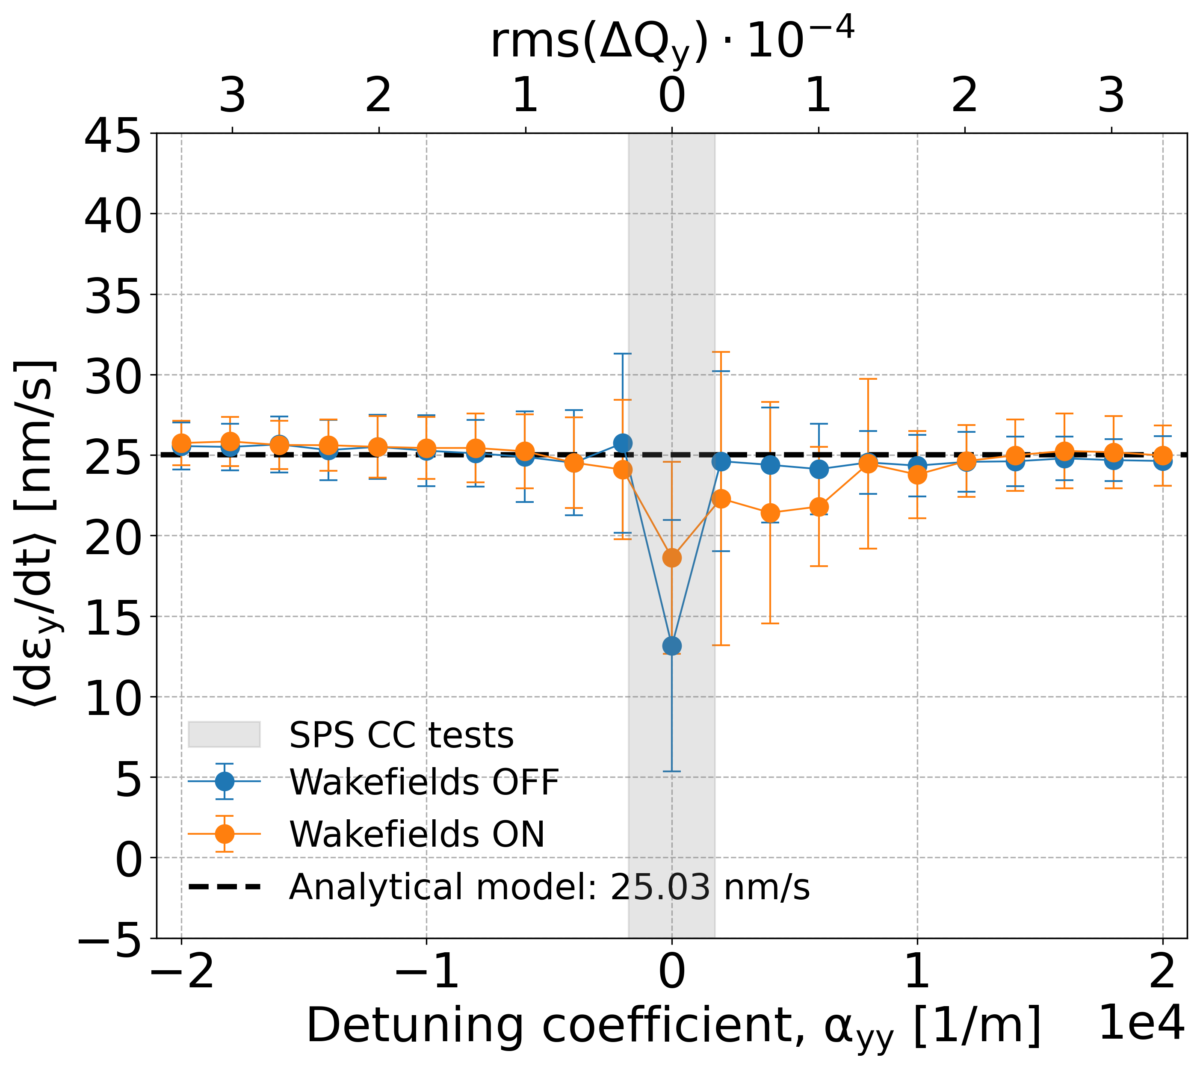
\includegraphics[width=1\textwidth]{images/Ch7/deyRates_final_2018_AN_sps_270GeV_PN1e-8_200MHz_y-plane_QpxQpy5e-1_6D_Nb5e5_intensity3e10_ayyScan_wakesON_vs_OFF_vs_TuneSpreadvsExpectedSPS_200MHz.png}
        \caption{Amplitude noise}
        %\label{fig:add_label_here}
    \end{subfigure}
    \hfill
    \begin{subfigure}[t]{0.45\textwidth}
        \centering
        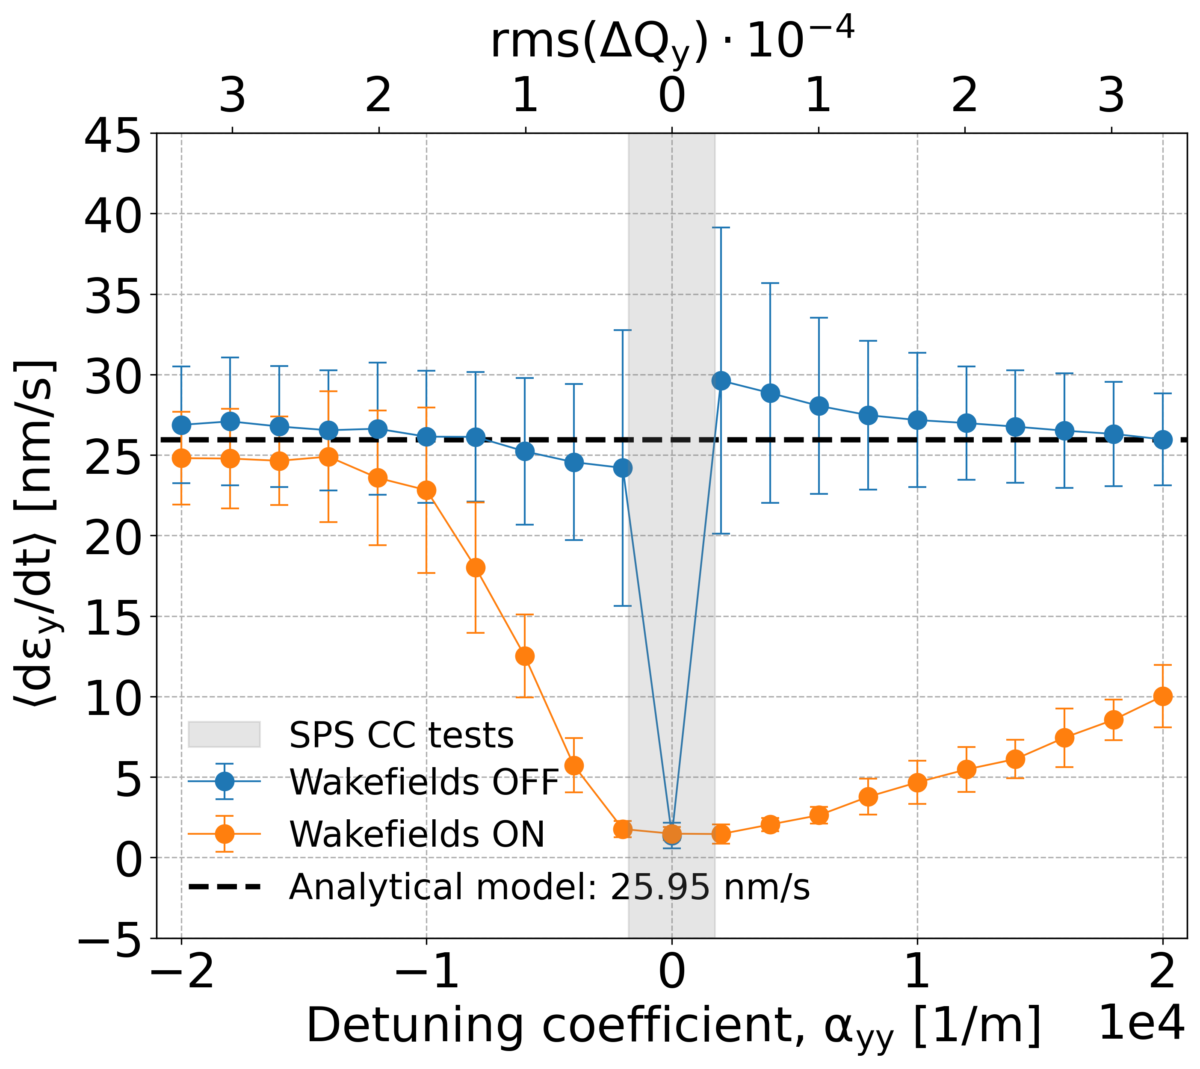
\includegraphics[width=1\textwidth]{images/Ch7/deyRates_final_2018_PN_sps_270GeV_PN1e-8_200MHz_y-plane_QpxQpy5e-1_6D_Nb5e5_intensity3e10_ayyScan_wakesON_vs_OFF_vs_TuneSpreadvsExpectedSPS_200MHz.png}
        \caption{Phase noise}
        %\label{fig:add_label_here}
    \end{subfigure}
    \hfill
     \caption{Transverse emittance growth driven by CC RF noise at $\CCfrequency=$200\,MHz without (blue) and with (orange) the impedance effects.} % bunch passage
     \label{fig:CC_200MHz_amplitude_phase_noise}
 \end{figure}

 Comparing Fig.~\ref{fig:CC_200MHz_amplitude_phase_noise} (left) and Fig.~\ref{fig:study_1_2018_paramters_AN} it becomes evident that the behavior of the amplitude noise induced emittance growth is consistent for noise at 200 and 400\,MHz (both with and without wakefields). In both cases there is no amplitude detuning dependent suppression of the emittance growth while the obtained growth rates agree very well with the theoretical predictions from Eq.~\eqref{eq:dey_an}.
 
 Comparing Fig.~\ref{fig:CC_200MHz_amplitude_phase_noise} (right) and Fig.~\ref{fig:MD_2018_impedance_simulations} it can be seen that emittance growth driven by $\CC$ phase noise in the absence of wakefield kicks (blue) is in excellent agreement for noise at 200 and 400\,MHz except for the case with zero amplitude detuning, $\alpha_\mathrm{yy}=0$. It is already discussed, that for $\CCfrequency$=400\,MHz the observed emittance growth of $\sim 15$\,nm/s is a result of the geometric distortion of the beam caused by the $\CC$ kick. This geometric distortion is minimised when the frequency of the $\CC$ kick equals the one of the main RF system hence the almost zero emittance growth observed for the phase noise at 200\,MHz. 

 Repeating the last comparison but in the presence of wakefield kicks (orange) it can be seen that emittance growth driven by $\CC$ phase noise is in good agreement with the results for noise at 200 and 400\,MHz. The suppression of the emittance growth, which depends on the amplitude detuning, is observed in both cases. However, in the case of phase noise at 200\,MHz the suppression factor reaches up to a factor of 10 instead of just 4-5 in the case of noise at 400\,MHz. The enhanced effect of suppression in the case where the $\CC$ has the same frequency with the main RF system of the machine and thus the headtail mode 0 is dominant provides an additional argument that the emittance growth suppression from the beam coupling impedance is associated to that mode. To this end, as a next step the emittance growth induced by a pure dipolar noise is studied.


 %Comparing Fig.~\ref{fig:CC_200MHz_amplitude_phase_noise} (right) and Fig.~\ref{fig:MD_2018_impedance_simulations} it can be seen that emittance growth driven by $\CC$ phase noise in the presence of wakefield kicks (orange) is in good agreement for noise at 200 and 400\,MHz. 


\subsection{Pure dipolar noise}\label{subsec:dipole_noise}
To validate that the effect of the suppression of the noise-driven emittance growth from the beam coupling impedance is associated with the dipolar motion (headtail mode 0), the same simulations as in the previous part were conducted but instead of the longitudinally dependent noise kicks a pure dipolar noise kick was applied on the beam. The dipolar noise kick was modeled by the transformation of Eq.~\eqref{eq:external_noise_kicks} for $A=10^{-8}$ which corresponds to a power spectral density of 3.36\,$\mathrm{rad^2/Hz}$. The noise strength was scaled such as it results in $\sim$ 25 nm/s to be comparable with the initial studies presented in Section~\ref{sec:first_obs_suppression}.

Figure~\ref{fig:study_5_dipole_noise} shows the noise-induced vertical emittance growth as a function of amplitude-dependent tune spread with and without the presence of wakefield kicks. One can see that in the absence of wakefields (blue) the behavior of the dependence of the growth rates on the amplitude detuning matches the one obtained from $\CC$ RF phase noise kicks (see Figs.~\ref{fig:study_1_2018_paramters_AN} and~\ref{fig:CC_200MHz_amplitude_phase_noise} (right)). However, now, due to the absence of any geometric distortion for $\alpha_\mathrm{yy}=0$ there is zero emittance growth as one would expect from the fact that the models that predict the emittance growth are not valid for zero tune spread.

In the presence of wakefield kicks (orange) a very strong suppression of the emittance growth is suppressed which reaches up to a factor of 10 for the small values of amplitude detuning (within the gray area which indicates the tune spread present in the SPS during the 2018 $\CC$ experiments). The fact that the suppression of the emittance growth intensifies in the presence of dipolar noise, is a way to infer the association of the phenomenon with the headtail mode 0.

\begin{figure}[!h] % cernbox/=/pyheadtail_data/final_for_thesis/2018_conditions/study_5_dipole_nois
    \centering         
    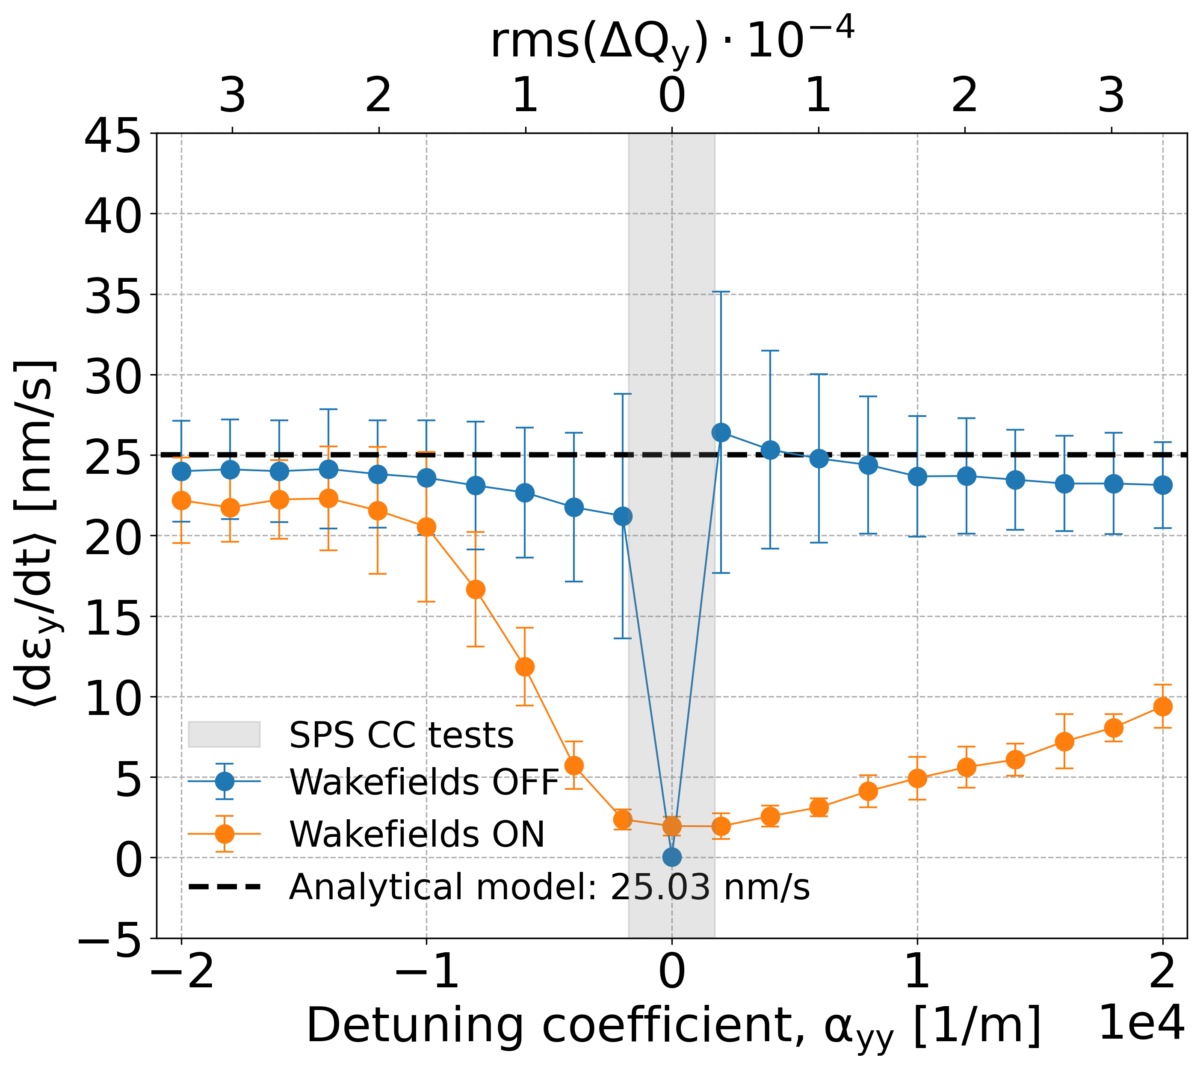
\includegraphics[width=0.85\textwidth]{images/Ch7/deyRates_final_2018_dipolar_noise_sps_270GeV_DipoleNoiseSQRT1e-8_y-plane_QpxQpy5e-1_6D_Nb5e5_intensity3e10_ayyScan_wakesON_vs_OFF_vs_TuneSpreadvsExpectedSPS.png}
        \caption{Transverse emittance growth driven by a pure dipolar noise kick without (blue) and with (orange) the impedance effects.}
        \label{fig:study_5_dipole_noise}
 \end{figure}



\subsection{Sensitivity to linear chromaticity}\label{subsec:chroma_scan}
The PyHEADTAIL simulations discussed up to now, cover the case for linear chromaticity $Q^\prime_{x,y}=0.5$ which is believed to be the case for the emittance growth measurements in SPS in 2018. Here, the suppression of the noise-induced emittance growth in the presence of the SPS impedance is investigated for different values of linear chromaticity to improve the understanding of the effect. In particular, the following values were studied: $Q^\prime_{x,y}=0.0, 0.5, 1.0, 2.5, 5.0$. It can be seen, that the study is limited to small positive chromaticity values following past experimental chromaticity scans for emittance growth studies,  $Q^\prime_{x,y}< 10.0$~\cite{Antoniou:2649815, Calaga:1451286}. An additional reason for not extending the study to the negative chromaticity values is that they would lead to beam instabilities.
% Note 1: The expereimental scan of the linear chromaticity scan from 0 to 7 (rama's paper), ipac2012.
% Note 2: if needed you can prove that the beam is unstable with the formula of Sacherer.

The simulations for this subsection were performed using the setup and the parameters of Section~\ref{sec:first_obs_suppression}. This means, that the study took place in the presence of $\CC$ RF phase noise kicks at 400\,MHz, with and without including the SPS imepdance model. The results of the scan in $Q^\prime_{x,y}$ are displayed in Fig.~\ref{fig:study_6_chroma_scan} where each subfigure pictures the results for each chromaticity value independently. The corresponding values are shown in the captions. 

\begin{figure}[htp]
    \centering
    \begin{subfigure}{.45\textwidth}
        \centering
        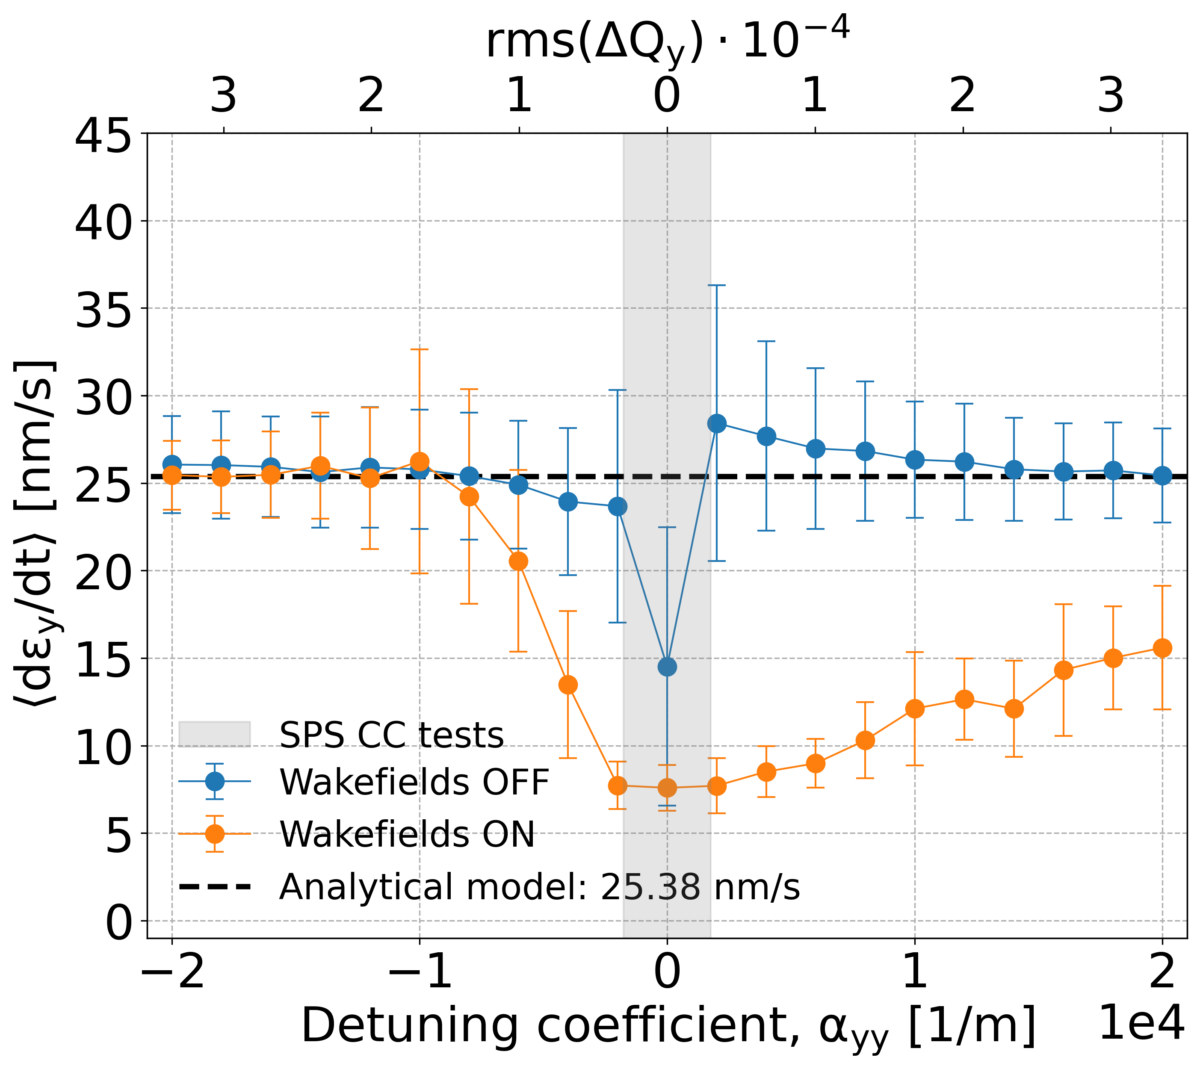
\includegraphics[width=.95\linewidth]{images/Ch7/Qpx0.png}  
        \caption{$Q^\prime_{x,y}$=0.0}
        \label{fig:study_6_chroma_scan_Qpxy0}
    \end{subfigure}
    \begin{subfigure}{.45\textwidth}
        \centering
        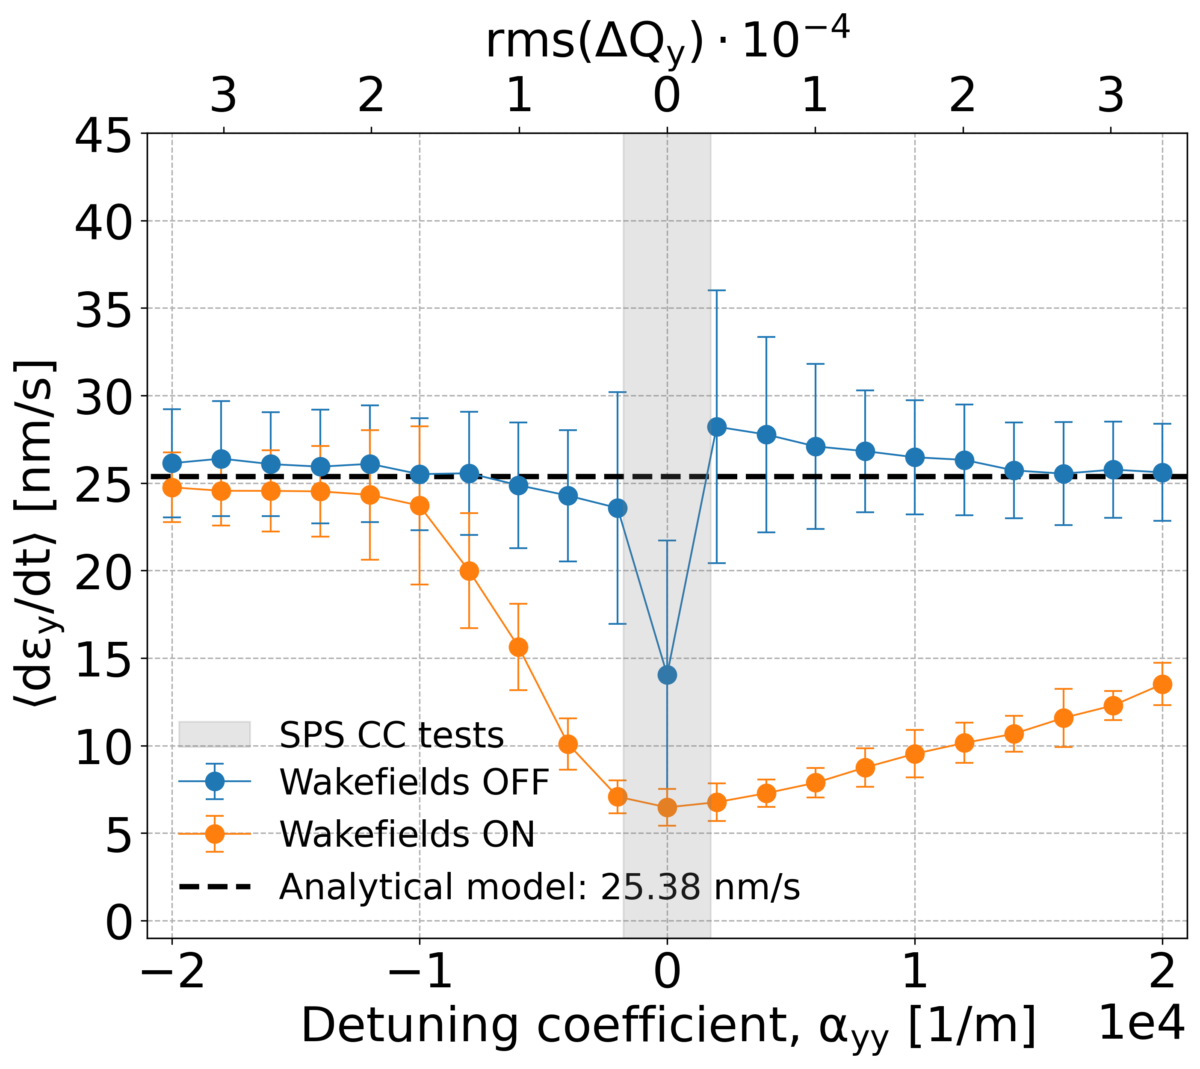
\includegraphics[width=.95\linewidth]{images/Ch7/deyRates_final_2018_PN_sps_270GeV_PN1e-8_400MHz_y-plane_QpxQpy5e-1_6D_Nb5e5_intensity3e10_ayyScan_wakesON_vs_OFF_vs_TuneSpreadvsExpectedSPS.png}
        \caption{$Q^\prime_{x,y}$=0.5}
        \label{fig:study_6_chroma_scan_Qpxy5e-1}
    \end{subfigure}
    \begin{subfigure}{.45\textwidth}
        \centering
        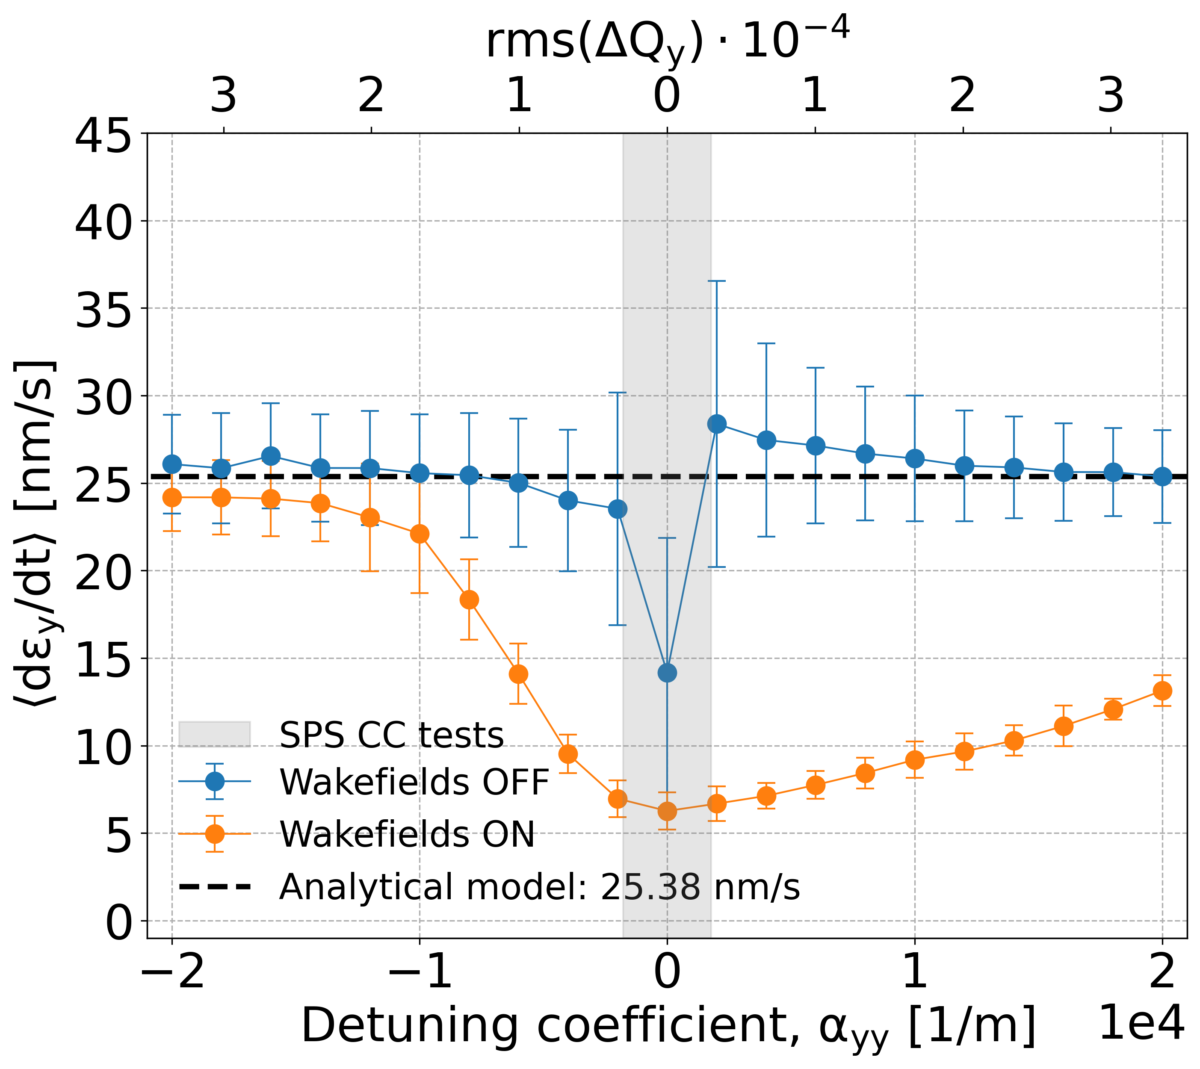
\includegraphics[width=.95\linewidth]{images/Ch7/Qpx1.png}  
        \caption{$Q^\prime_{x,y}$=1.0}
        \label{fig:study_6_chroma_scan_Qpxy1}
    \end{subfigure}
    \begin{subfigure}{.45\textwidth}
        \centering
        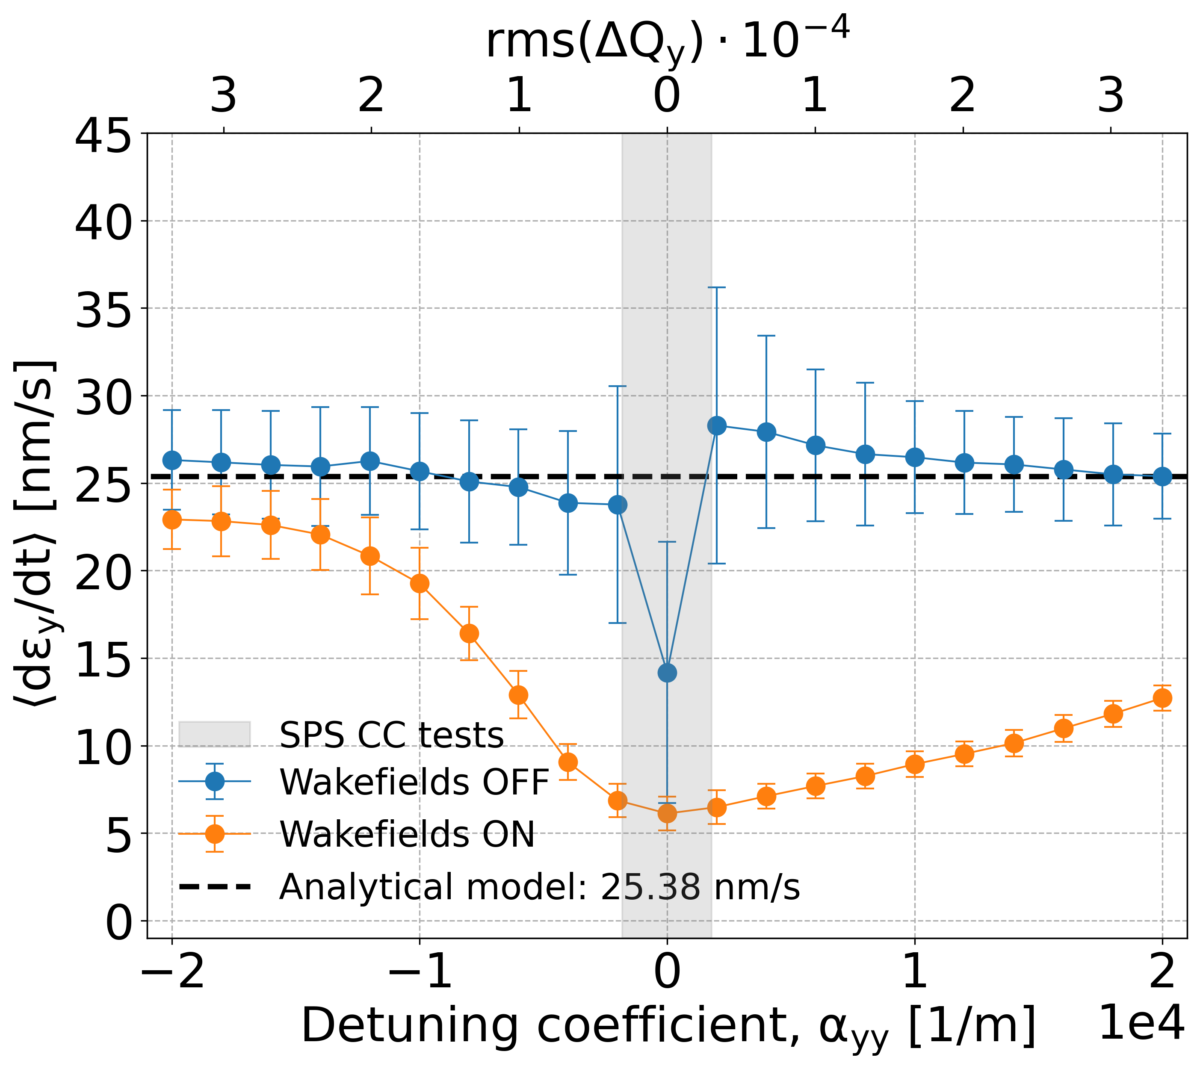
\includegraphics[width=.95\linewidth]{images/Ch7/Qpx25e-1.png}  
        \caption{$Q^\prime_{x,y}$=2.5}
        \label{fig:study_6_chroma_scan_Qpxy25e-1}
    \end{subfigure}
    \begin{subfigure}{.45\textwidth}
        \centering
        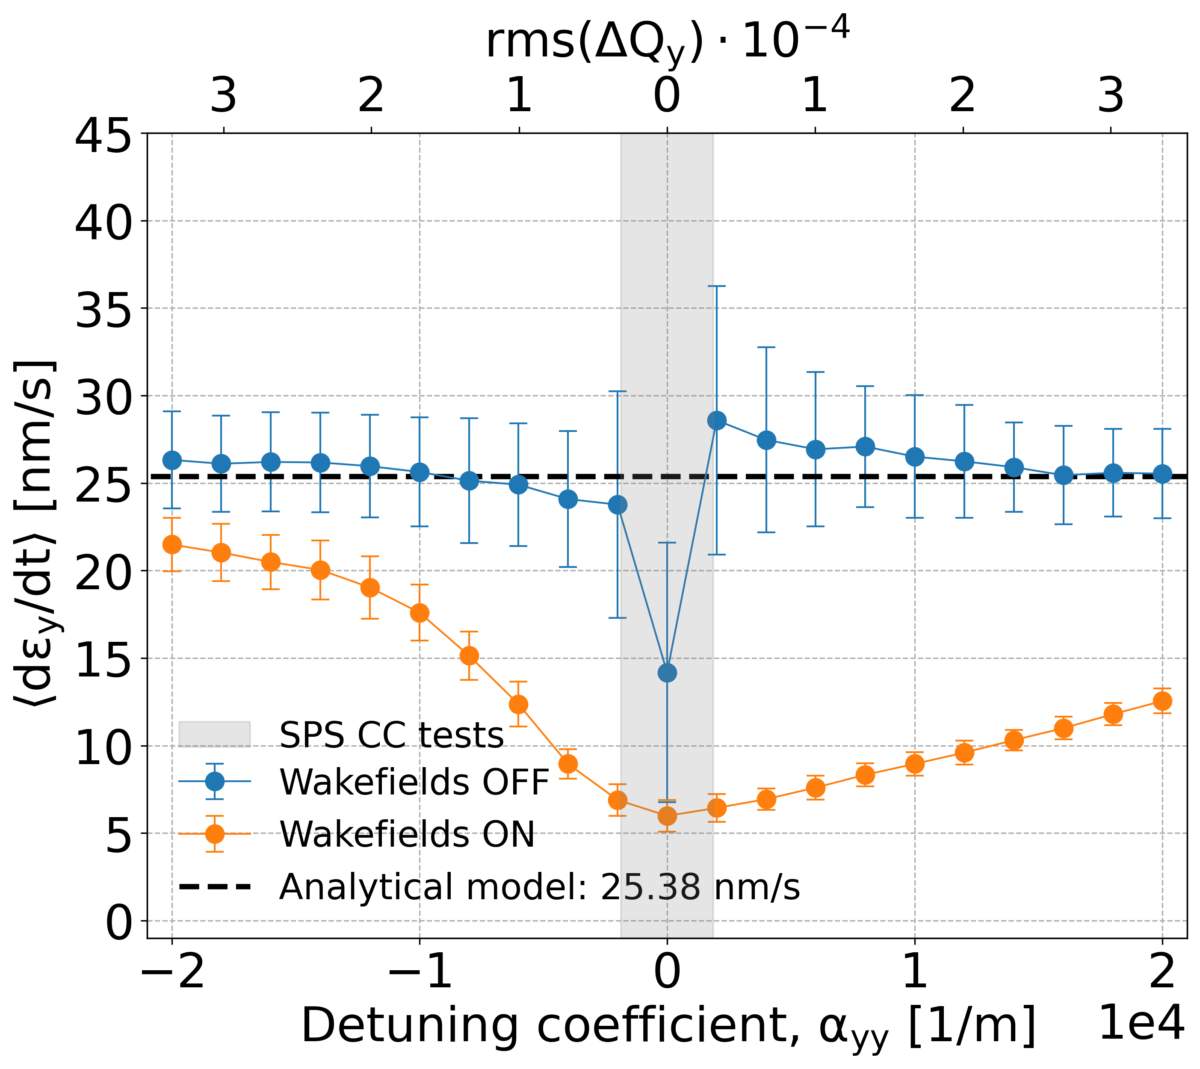
\includegraphics[width=.95\linewidth]{images/Ch7/Qpx5.png}  
        \caption{$Q^\prime_{x,y}$=5.0}
        \label{fig:study_6_chroma_scan_Qpxy5}
    \end{subfigure}
    \caption{FIGURE CAPTION}
    \label{fig:study_6_chroma_scan}
    \end{figure}


where each subfigure pictures the results for 


The PyHEADTAIL simulation results of the scan in $Q^\prime_{x,y}$ are displayed in Fig. . 

Here, the suppression of the noise induced emittance growth in the presence of the SPS impedance is investigated for different values of linear chromaticity.

The PyHEADTAIL results of the scan in the linar chromaticity values, $Q^{\prime}_y$ are displayed in Fig


Wiuthout wakefeilds no dependnece on amplitude deuting . this observations are in agreement with the ones made for subsection 1-2.

\subsection{Disentangle quadrupolar and dipolar contribution}\label{subsec:quad_vs_dipole}


\section{Suppresion mechanism}\label{sec:suppression_mechanism}
\subsection{Past studies with beam-beam interactions}\label{subsec:past_studies_impedance_suppression_BB}
\subsection{Intensity scans}
\subsection{Schottky noise spectra}
\subsection{Studying the motion of the centroid - decoherence}
PyHEADTAIL simulations of the evolution of the centroid vs emittance for difference values os amplitude detuning. 


\section{Towards HL-LHC case}
\subsection{Damper}
Comment on the 200 MHz

I might make a comment:
% From 30 months progress report doctoral: cernbox/Documents/education/cern/doctoral/30months_progress_report
Detailed studies with PyHEADTAIL showed that the emittance growth suppression can reach up to a factor of 2-4 for crab cavity phase noise when the bunch length is longer than the cavity wavelength, which was the case for the SPS experiments. However, for short bunch lengths, which will be the case in the HL-LHC, the suppression factor was found to be similar to the case of pure dipolar noise reaching a factor of 10. The scope of this project is also to characterize the impact of the crab cavities in the long-term emittance evolution in HL-LHC. Thus, the interplay of the transverse impedance and the transverse feedback system, which is planned to suppress the crab cavity noise induced emittance growth in HL-LHC, started being investigated. The first simulation results indicate that the emittance suppression from the feedback system is not affected by the impedance, due to the much faster damping time of the former.

\section{Conclusions}
% From 30 months progress report doctoral: cernbox/Documents/education/cern/doctoral/30months_progress_report
You need to modiy it a bit.
In a second step, simulations including the complete transverse impedance model of SPS, which was not taken into account so far, were performed with PyHEADTAIL. It was found that the transverse impedance can suppress the crab cavity noise induced emittance growth once the coherent tune, which is shifted by the impedance, moves out of the incoherent tune spectrum. It turns out that the decoherence process is slowed down and thus the noise induced emittance growth is suppressed. This mechanism, which has been observed in the past as a result of beam-beam interactions, is related to the transverse dipole oscillation of the beam. To this end the suppression is not observed for amplitude but only for phase noise induced emittance growth.

\chapter{Simple model of describing the decoherence suppression from impedance}
\section{Motivation}\label{sec:motivation_md_2022}
As discussed in the previous chapter, PyHEADTAIL simulations including the SPS impedance model suggest that the beam coupling impedance leads to an effective suppression of the $\CC$ RF phase noise induced emittance growth through the separation of the coherent tune from the incoherent spectrum. This suppression, which is related to the coherent (dipole) motion, can reach up to a factor of 4-5 for the experimental conditions of the first experimental campaign with $\CC$s that took place in the SPS in 2018, which seems to be the explanation for the experimental observations (see Section~\ref{sec:MD5_overview}).

This suppression effect has never been observed before. To this end, another experimental campaign took place in the SPS in 2022 where the main objective was to validate experimentally the above-mentioned suggested emittance growth suppression mechanism. If successful, it would constitute the first experimental investigation and validation of this effect. Moreover, achieving a good understanding of the 2018 results is essential for developing confidence in the theoretical model and its predictions for the HL-LHC.

The experimental campaign of 2022 was organised in two proof-of-concept experiments. The first experiment was carried out in the presence of phase noise in the $\CC$ RF system. The second experiment took place with a pure dipolar noise source: the beam transverse damper. This chapter reports on the preparation, the methodology, and the results of these experiments.

\section{Experiment with CC as noise source}\label{sec:cc_md_2022}
Due to the preceding PyHEADTAIL simulations which provided strong evidence that the observed discrepancy between the 2018 measurements and the theoretical predictions could be explained by the beam transverse impedance additional machine time was dedicated to emittance growth studies with $\CC$ in the SPS in 2022. The time allocated for the $\CC$ experiment was limited to about 10 hours since many different studies have to take place in the SPS during the year. Taking into consideration the time needed for the setup and the $\CC$ calibration the time available for the emittance growth measurements is reduced even more. To this end, measurement repeatability is limited and the experimental procedure had to be carefully planned in advance.
% Also you can add that each point in the emittance growth studies needs about 30-40 min.

\subsection{Machine and beam configuration}\label{sec:cc_md_2022_parameters}
The emittance growth measurements in 2022 were performed in "coast" mode at 270\,GeV following the same setup as in 2018 (see Section~\ref{sec:exp_setup_2018}) and very similar machine and beam conditions. The most relevant parameters are listed in Table~\ref{tab:machine_beam_param_2022}. 

The linear chromaticity was corrected to about zero units in both the horizontal and vertical planes. That was a result of miscommunication with the operator team of the SPS machine as the desired value was between 0.5 and 1.0. However, the analysis of the PyHEADTAIL simulations in Section~\ref{subsec:chroma_scan} showed that the sensitivity of the emittance growth suppression to the linear chromaticity values (for small positive values) is expected to be insignificant. 

On the grounds that the last three (out of four) bunches used in 2018 expereimental campain were unstable, in 2022 the experiment was carried out with a single bunch. This choice allowed also to have better control on the beam conditions, avoiding possible effects from interactions between the bunches \footnote{Even though these effects should be insignificant due to the large bunch spacing, see Table~\ref{tab:machine_beam_param_2018}.}.

\begin{table}[!hbt]
	\begin{minipage}{\textwidth}
      \begin{centering}
   \caption{Main machine and beam parameters for the emittance growth studies with CCs in SPS in 2022.}
	\begin{tabu} to \textwidth {X[c,m] X[0.5c,m] X[0.5c,m] X[0.01c,m]}
		&&& \\[-6mm]
		\toprule \toprule
		\multicolumn{2}{l}{\textbf{Parameter}} &
		\multicolumn{2}{c}{\textbf{Value}} \\
		\bottomrule
      \multicolumn{2}{l}{Beam energy, $\symE$} & \multicolumn{2}{c}{270\,GeV} \\
      \multicolumn{2}{l}{Main RF voltage / frequency,  $\VRF$ / $\fRF$}  & \multicolumn{2}{c}{5\,MV / 200.39\,MHz} \\ %200.3945
      \multicolumn{2}{l}{Horizontal / vertical betatron tune, $\Qx$ / $\Qy$}  & \multicolumn{2}{c}{26.13 / 26.18} \\
      \multicolumn{2}{l}{Horizontal / vertical first order chromaticity, $\Qpx$ / $\Qpy$}  & \multicolumn{2}{c}{ $\sim$ 0.0-0.5 / $\sim$ 0.0-0.5} \\
      \multicolumn{2}{l}{Synchrotron tune, $Q_s$}  & \multicolumn{2}{c}{0.0051} \\
      \multicolumn{2}{l}{$\CC 1$ voltage / frequency, $\VCC$ / $\fCC$}  & \multicolumn{2}{c}{1\,MV / 400.78\,MHz} \\
      \multicolumn{2}{l}{Number of protons per bunch, $\Nb$} & \multicolumn{2}{c}{3 $\times 10^{10}$ p/b$^\ast$} \\
      \multicolumn{2}{l}{Number of bunches}  & \multicolumn{2}{c}{1} \\
      \multicolumn{2}{l}{Bunch length, 4$\sigmat$}  & \multicolumn{2}{c}{1.83 \,ns$^\ast$}\\
      \multicolumn{2}{l}{Horizontal / vertical normalised emittance, $\emitx$ / $\emity$}  & \multicolumn{2}{c}{2\,$\mathrm{\mu m}$ / 2\,$\mathrm{\mu m^\ast}$}\\
      \multicolumn{2}{l}{Horizontal / vertical rms tune spread, $\Dqxrms$ / $\Dqyrms$}  & \multicolumn{2}{c}{2.02 $\times 10^{-5}$ / 2.17 $\times 10^{-5}$ $^\ddagger$}\\
      \bottomrule
	\end{tabu}
   \label{tab:machine_beam_param_2022}
   \end{centering} \footnotesize{$^\ast$ These values corresponds to the requested intial value at the start of each coast.  \\ $^\dagger$ This value corresponds to the average rms measured bunch length over all the coasts of 2022. \\$^\ddagger$ Here the rms betatron tune spread includes only the contribution from the detuning with amplitude present in the SPS machine. More details along with the calculations for the listed values can be found in Appendix~\ref{app:detuning_with_amplitude}.}
   \end{minipage}
\end{table}
% For bunch length: cernbox/2022/SPS_MDs_2022/cc_md_16May2022/longitudinal_profiles/visualise_pickle.ipynb

The average bunch length (over all settings) was measured to be about $4\sigma_t$ = 1.83\,ns. During the coasts, an increase in the bunch length of $\sim$5~$\%/h$ on average for each setting was observed. This small increase agrees with what is usually observed in the SPS in coast and will not be taken into consideration in the following analysis. The individual plots illustrating the evolution of the bunch length as measured with the Wall Current Monitor (introduced in Section~\ref{sec:ABWLM_WallCurrentMonitor}) during the experiment are presented in Appendix~\ref{sec:bunch_length_measurements_2022}. Finally, looking at the dependence of the emittance growth suppression by the impedance on the bunch length in Fig.~\ref{fig:study_10_bunch_length} it is evident that the bunch length of $4\sigma_t$ = 1.83\,ns belongs to the regime of the strong suppression. This is important as it optimizies the experimental conditions to observe the impedance effects on the noise-induced emittance growth. \textcolor{red}{The last sentence needs to be refined. See comment from Andy.}

The intensity was set to $3 \times 10^{10}$ protons to be in agreement with the experiment of 2018. During the coasts of the 2022 experiment almost zero losses were observed. Therefore, the evolution of the intensity during the coasts will be not considered in the following.


\textbf{CC RF noise}\\
The noise injected in the $\CC$ RF system was again a mixture of phase and amplitude noise. The noise excitation extended from DC up to 10\,kHz and thus the noise was applied on the first betatron sideband only, at $\sim$8\,kHz. The power spectral density values at $\sim$8\,kHz of the four different levels of artificial noise that were used in the experiment are listed in Table~\ref{tab:noise_settings_2022}. By looking at the table, it becomes evident that the contribution of amplitude noise to the total emittance growth was found to be small (about 7$\%$). To this end, in the post-processing of the 2022 data, the introduction of the effective phase noise (see Section~\ref{sec:injected_RF_noise}) is not required. In the following, the measured growth rates will be displayed as a function of the measured RF phase noise only. This choice is also justified by the fact that the objective of the 2022 experimental campaign with $\CC$s is to mainly reproduce the qualitative expected bahevior from the impedance and not the exact values. This is discussed further in the next sections of this chapter.

% I don't have the data to plot the spectra. Only screenshots in the logbook.


% Note 1: Noise level values from the logbook.
% Note 2: Analysis and percentages: /2022/SPS_MDs_2022/cc_md_16May2022/roundA_online_analysis_ws/summary_plots/for_thesis/cc_md_analysis_noise_scan_for_thesis.ipynb
\begin{table}[!hbt]
	\centering
   \caption{Phase and amplitude noise levels injected in the CC RF system for the emittance growth studies of 2022 along with the analytically expected growths. The listed noise values correspond to the power spectral density values at the first betatron sideband, $f_b$, at $\sim$8\,kHz. The analytical emittance growth rates were computed using Eq.~\eqref{eq:dey_an} and~\eqref{eq:dey_pn} for bunch length of $4\sigma_t$=1.83\,ns.}
	\begin{tabu} to \textwidth { X[c,m] X[c,m] X[c,m] X[c,m] X[c,m]}
		&&&& \\[-6mm]
		\toprule \toprule
		\multicolumn{1}{l}{} &
		\multicolumn{2}{c}{$\mathbf{10\,\boldsymbol{\log}_{10} \mathcal{L}(f)}$ \textbf{[dBc/Hz]}} & \multicolumn{2}{c}{\textbf{Analytical } $\mathbf{d \boldsymbol{\epsilon}_y/dt \ [\boldsymbol{\mu} m/h]}$} \\
		\bottomrule
      \multicolumn{1}{l}{} & 	\multicolumn{1}{c}{\textbf{Phase noise}} & \multicolumn{1}{c}{\textbf{Amplitude noise}} & \multicolumn{1}{c}{\textbf{Phase noise}} & \multicolumn{1}{c}{\textbf{Amplitude noise}} \\
      \midrule
      \multicolumn{1}{l}{Level 1}  & \multicolumn{1}{c}{-115.2} & \multicolumn{1}{c}{-124.6} & \multicolumn{1}{c}{1.64} & \multicolumn{1}{c}{0.16} \\
      
      \multicolumn{1}{l}{Level 2}  & \multicolumn{1}{c}{-109.5} & \multicolumn{1}{c}{-120.5} & \multicolumn{1}{c}{6.11} & \multicolumn{1}{c}{0.42}\\

      \multicolumn{1}{l}{Level 3}  & \multicolumn{1}{c}{-104.7} & \multicolumn{1}{c}{-116.0} & \multicolumn{1}{c}{18.44} & \multicolumn{1}{c}{1.19} \\

      \multicolumn{1}{l}{Level 4}  & \multicolumn{1}{c}{-100.1} & \multicolumn{1}{c}{-111.0} & \multicolumn{1}{c}{53.19} & \multicolumn{1}{c}{3.76} \\ 
      \arrayrulecolor{black}\bottomrule
	\end{tabu}
   \label{tab:noise_settings_2022}
\end{table}



\textbf{CC1 instead of CC2}\\
In the 2022 campaign, $\CC$1 was used instead of $\CC$2 which was used in 2018. The reason behind this is that during the $\CC$ phase scan that was performed in 2022 to calibrate the $\CC$ phase offset (see Section~\ref{subsec:cc_calibration_2022}) $\CC$2 tripped systematically. The issue is associated with the change of the RF phase but fixing this problem would have been time-consuming which was not an option due to the very limited machine time of the MD. Therefore, for the measurements in 2022 $\CC$1 was used.
% CC2 tripped: see the entry of the logbook 4/5/2022, at 11:30:30 

\textbf{SPS Wire Scanners}\\
The emittance values were measured with the SPS Wire Scanners according to the procedure discussed in Section~\ref{subsec:sps_ws}. In particular, wire scanners SPS.BWS.51637.H and SPS.BWS.41677.V were used for measurements in the horizontal and vertical planes, respectively. For both devices the data points from the second photomultiplier were used (PM2) \footnote{Each Wire Scanner device is equipped with four PMs. Each one of them provides a better resolution of the amplitude signal of the secondary particles for a different regime. The choice of PM2 for the emittance growth studies in 2022 was done "online", during the experiment, by examining the obtained beam profiles.}. The beta functions of the respective plane at the locations of the wire scanners are 79.29\,m, and  60.75\,m. 
% The values of the beta functions were obtained from MADX: https://github.com/natriant/exploring_SPS/blob/master/madx_studies/optics_new_seq_after_LS2/output/twiss_thin_elements/find_beta_functions_at_locations.ipynb 

As explained erlier (see Section~\ref{subsec:sps_ws}) during each measurement with the wire scanners the beam profile is acquired two times as the wire crosses the beam in the forward direction (IN scan) and then in the reverse direction (OUT scan). For the experiment of 2022, the OUT scan was performed just 200\,ms after the IN scan. However, it was observed that there are significant discrepancies between the measurements from IN and OUT scan, which in some cases reached up to 1\,$\mathrm{\mu m}$. By looking at the acquired profiles no reason was found to exclude or not one of the two scans. A significant effort was done with the wire scanner experts during the emittance growth experiment trying to mitigate this effect without success due to limitations on the hardware of the current instrument. Therefore, it was decided that the post-process analysis would be performed taking into account only the IN scan measurements since they appeared to have systematically less fluctuation than in the OUT scan.

It is worth commenting that this issue was not observed in the 2018 measurements. A possible explanation is that the wire scanner acquisitions of 2022 provide lower number of points to reconstruct the bunch profiles (compare Figs.~\ref{fig:WS_example_V_profile} against~\ref{fig:WS_example_profiles_V_2022}) increasing the uncertainty of the obtained emittances. The reason behind this, is that between 2018 and 2022 the wire scanners had undergone an upgrade which increased their speed while crossing the bunch. A possible solution to this issue would be to reduce the speed of the wire for the emittance growth experiments in coast mode. This is currently in discussion with the team responsible for the wire scanners of the SPS.

% Evidence for the strong difference between IN and OUT https://docs.google.com/presentation/d/1QIaQNfqVWaI8cHGGgb5eeS7c_jdUMuxLqD_poHrOtH0/edit?usp=sharing

Last, the low emittance growth rates showed a significant sensitivity to the fluctuation of the wire scanner measurements. For this reason, for the low $\CC$ noise levels, long measurement times of about 30-40 minutes were needed.


%\textbf{Head-Tail monitor calibration}\\
%From the end of 2018 till the end of 2020, the CERN accelerator complex has undergone its second long shutdown in order to complete its scheduled upgrade program. Therefore, the calibration of the Head-Tail monitor was repeated to provide the normalisation factor required for the scaling of its reading (see Section~\ref{subsec:HT_post_process_CC}). The calibration factor was found to be 0.1037 in November 2021, as shown in Fig.~\ref{fig:HT_calibration_2022_levens} (slope value).

%\begin{figure}[!h] % Email communication with T. Levens on 8 November 2021.
%    \centering         
%    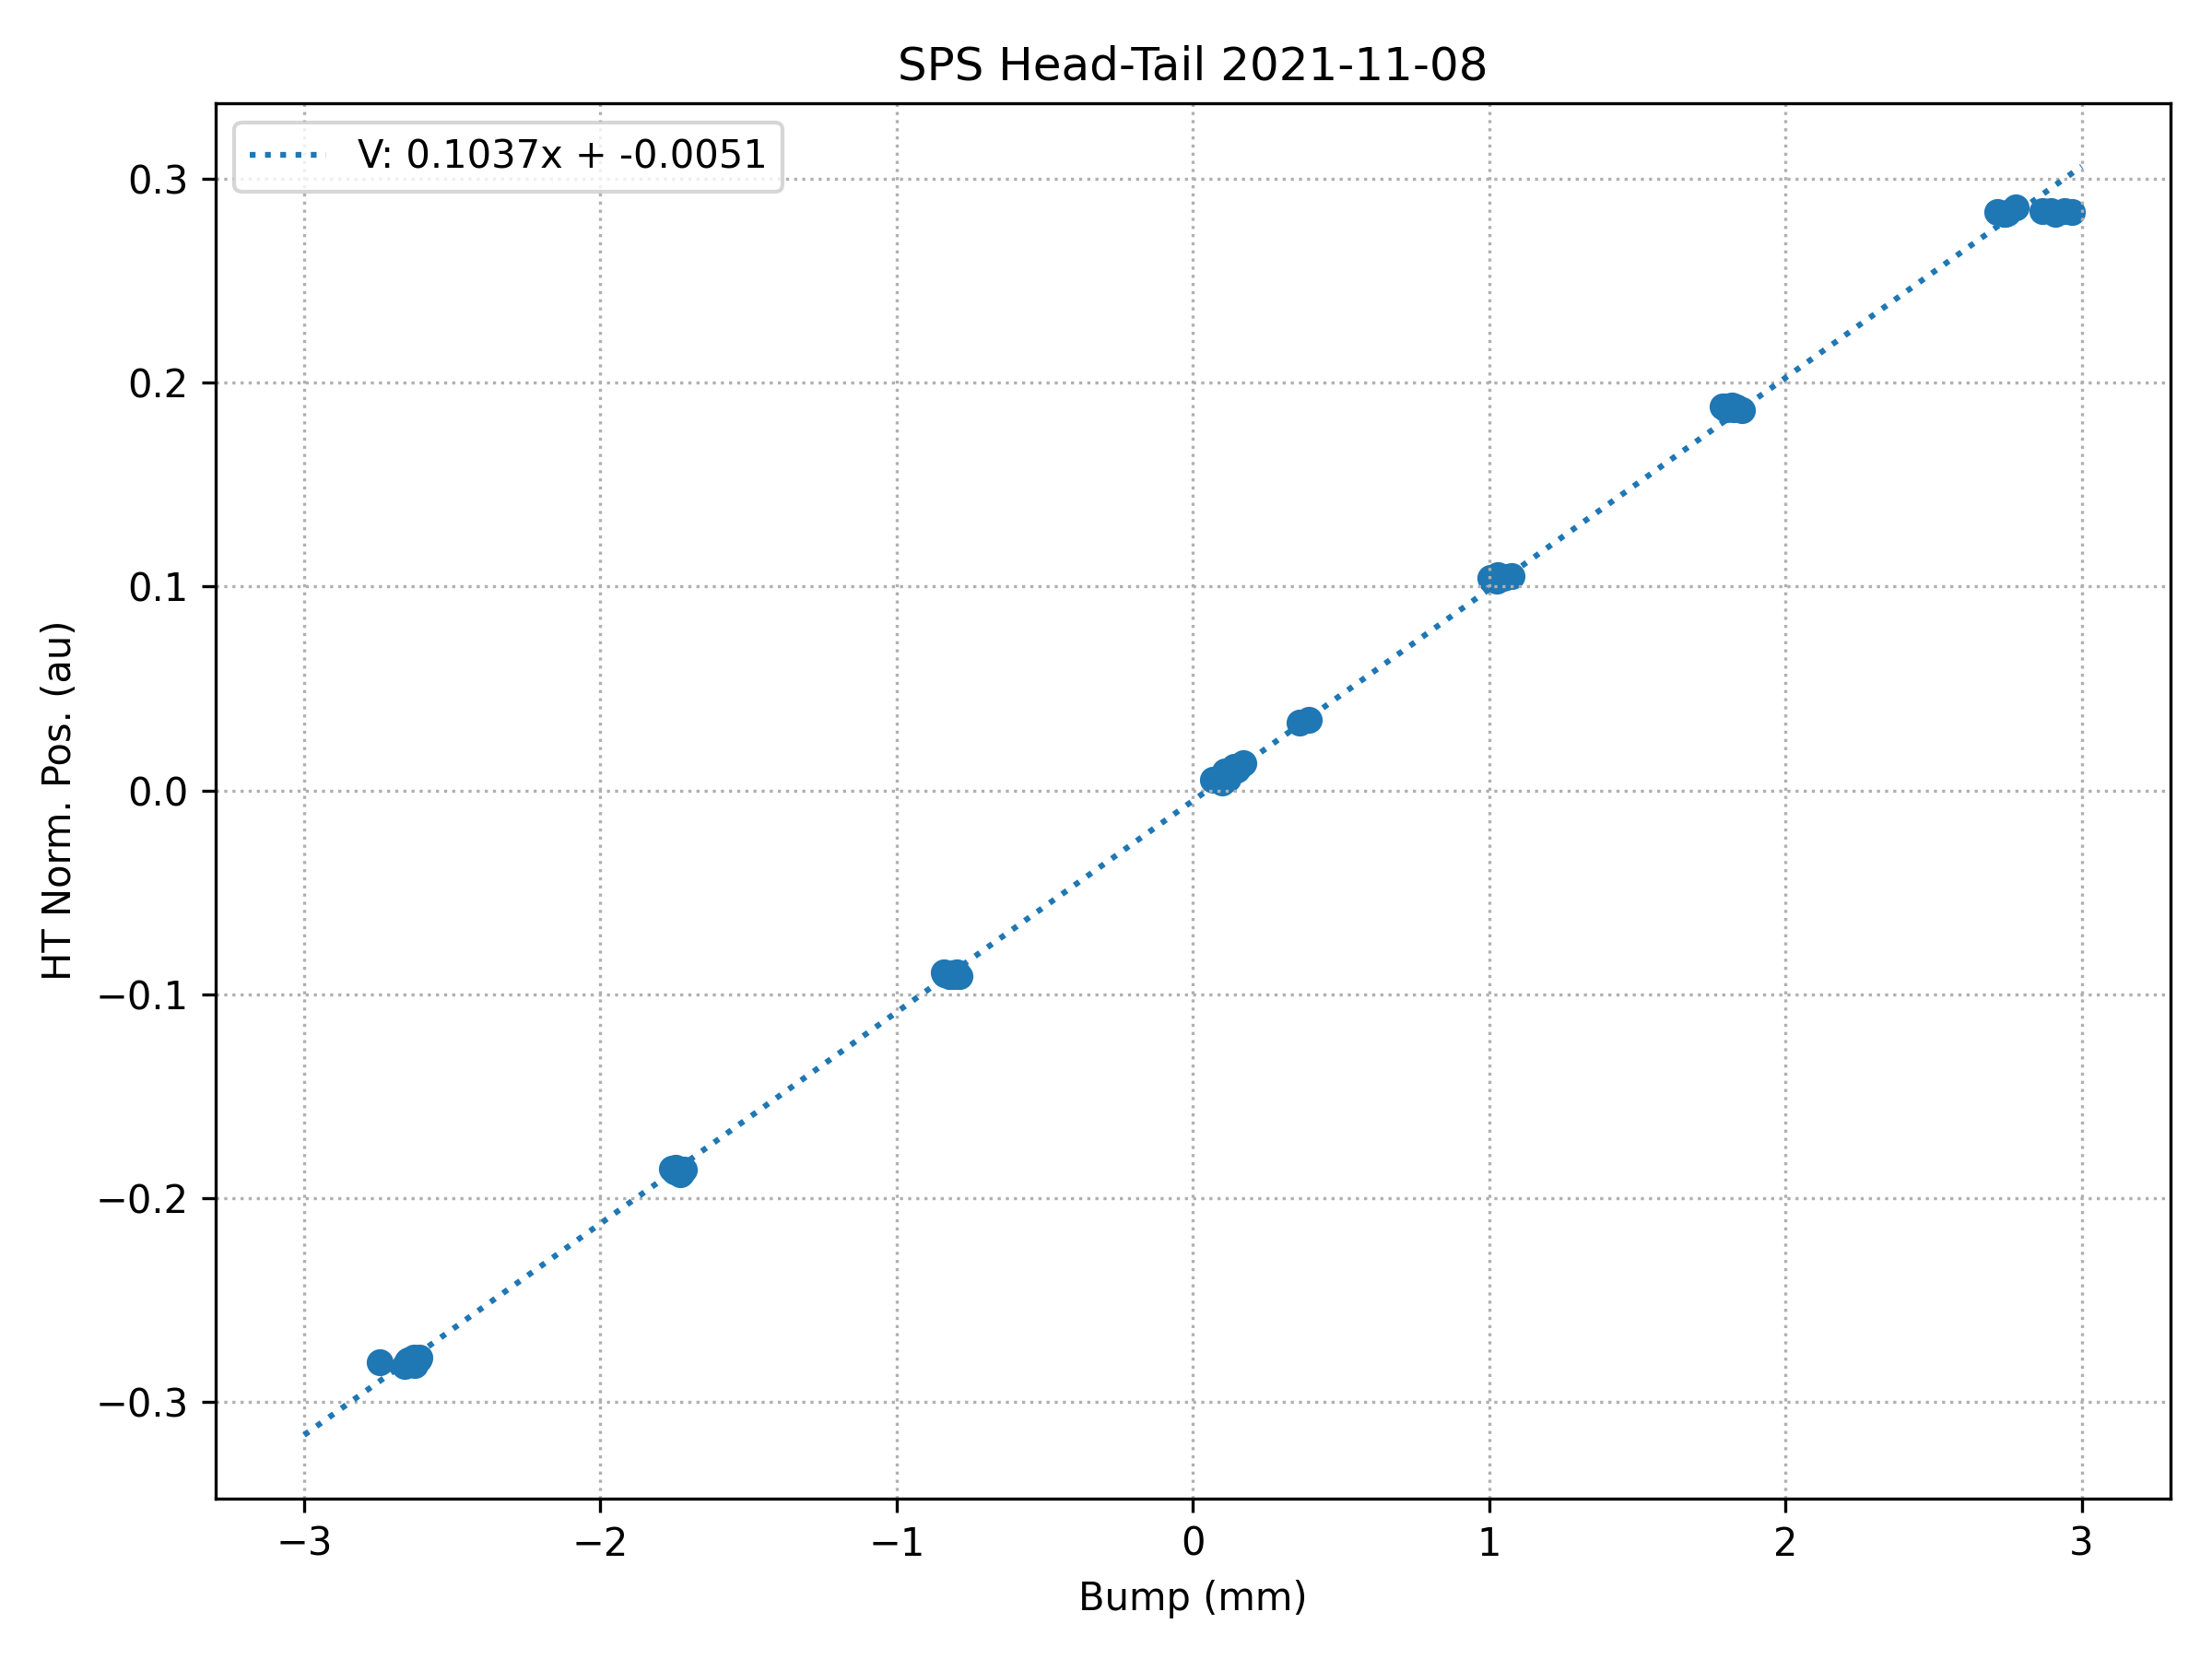
\includegraphics[width=0.7\textwidth]{images/Ch8/HT_monitor_calibration_2022.png}
%        \caption{The calibration was performed by T.~Levens by performing orbit bumps (around the reference orbit) and measuring the normalised position of the bunch in the vertical plane (plane of interest). The normalised position is obtained as the difference of the signal divided by the sum. More details on the calibration procedure are given in~\cite{PhysRevAccelBeams.22.112803}. This plot is courtesy of T.~Levens .}
%        \label{fig:HT_calibration_2022_levens}
% \end{figure}


\subsection{Experiment preparation and procedure}\label{sec:cc_md_2022_preparation}
\textbf{Objectives}\\
The available machine time ($\sim$ 10 hours) for the $\CC$ experiment of 2022 was split into two parts. For the first part, the objective was to measure the emittance growth with the same noise levels and conditions as in 2018 in order a) to reproduce the observed scaling of emittance growth (see Fig.~\ref{fig:MD5_summary_plot}) and b) to benchmark the expected suppression factor from PyHEADTAIL simulations with the impedance model. This will be referred to as $\CC$ Experiment A in the following.

The objective of the second part was to investigate the effects of impedance and amplitude detuning on the emittance growth from $\CC$ phase noise. The preceding analysis of the PyHEADTAIL simulations revealed a significant sensitivity of the emittance growth suppression on amplitude-dependent tune shift (e.g. Fig.~\ref{fig:MD_2018_impedance_simulations}). This behavior can be tested experimentally in the SPS with the use of the Landau octupole families, which allow for the introduction of controlled detuning with amplitude. A successful reproduction of this behavior would provide the proof-of-concept for the emittance growth suppression mechanism from the beam transverse impedance. This will be referred to as $\CC$ Experiment B in the following. It should be mentioned, that for this experiment the octupoles of the LOD family are employed as they act mostly in the vertical plane which is the plane of interest in this studies (vertical $\CC$ module which results in vertical emittance growth).

\textbf{Preparatory studies with PyHEADTAIL simulations}\\
In preparation for the $\CC$ experiments (A and B) the emittance growth in the presence of $\CC$ RF phase noise was simulated with PyHEADTAIL including the most up-to-date SPS impedance model~\cite{updated_sps_wakfields_model} as a function of different octupole strengths, $k_{\mathrm{LOD}}$. The beam and machine parameters are the ones reported in Table~\ref{tab:machine_beam_param_2022} which correspond to the experimental conditions of 2022. The emittance growth is induced by $\CC$ RF phase noise with a power spectral density of 1.68\,$\mathrm{rad^2/Hz}$ in the first betatron sideband which results in an emittance growth rate of about 25\,nm/s. It should be highlighted that this noise level is much stronger than the levels of the injected artificial noise used in the experiment, in order for the growth to be easily observed in the simulation time of just 2.5\,s. Therefore, the goal of the experiments was to reproduce the simulated suppression factor and behavior only and not the exact numbers. Finally, the simulation setup and the $\CC$ RF phase noise were simulated as discussed in Chapter~\ref{Ch:suppression_impedance}. 

The emittance growth was simulated over a range of twenty one $k_\mathrm{LOD}$ values equally spaced from -28.2\,$\mathrm{1/m^4}$ to +28.3\,$\mathrm{1/m^4}$. Nevertheless, in the simulations, no actual octupolar elements were used in order to avoid the excitation of resonances as discussed in Section~\ref{sec:first_obs_suppression}. Instead, following the preceding PyHEADTAIL simulations, the effect of LODs is introduced as a change in the phase advance of the individual particles depending on their individual actions and defined by the corresponding detuning coefficients. The study was performed for zero horizontal detuning coefficient, $\alpha_{xx}$=0 while the values of the vertical, $\alpha_{yy}$, and the cross-term, $\alpha_{yx}$, coefficients were estimated using MAD-X~\cite{madx}.

Figure~\ref{fig:pyheadtail_cc_impedance_2022_md_octupole_current} illustrates the dependence of the $\CC$ RF phase noise-induced emittance growth on the LOD strength, in the absence (blue) and the presence (orange) of the wakefields. The analytical prediction of the model Mastoridis--Baudrenghien is also given to facilitate the identification of the suppression factor from the impedance (horizontal black dashed line). As usual, in the absence of wakefields, there is a very good agreement between the simulation results and the theoretical predictions. In the presence of wakefields, the expected dependence on the tune spread appears. The rms tune spread values (shown on the secondary horizontal axis) are computed taking into account both the $\alpha_{\mathrm{yy}}$ and $\alpha_{\mathrm{yx}}$ coefficients using Eq.~\eqref{eq:rms_amplitute_detuning_3}.

% 1) Slides on computing the octupole current: https://docs.google.com/presentation/d/1VgGMqCevej4Eh7bjdGFSEPVI0zLxqB2S5FxLtFGhp2I/edit#slide=id.ge970b2a80a_0_16
The green and yellow areas indicate regimes where the octupoles require less than 200\,A and 400\,A respectively for their operation. The maximum operational current for the LODs in SPS is 400\,A. However, due to their planned continuous operation in multiple coasts, the LOD current should stay below 200\,A. The required current for the octupoles is computed from their strength, $k_\mathrm{LOD}$, using Eq.~\eqref{eq:I_vs_B3_relation_lof}


% /eos/user/n/natriant/pyheadtail_data/final_for_thesis/2022_conditions/CC1/deyRates_sps_270GeV_PN1e-8_400MHz_SPS_CC2_updatedWakes_y-plane_WakesOFF_vs_WakesON_new_QpxQpy0.5_6D_Nb5e5_intensity3e10Scan_vs_TuneSpreadvsExpectedSPS_octupole_current.png
\begin{figure}[!h] % Email communication with T. Levens on 8 November 2021.
   \centering         
   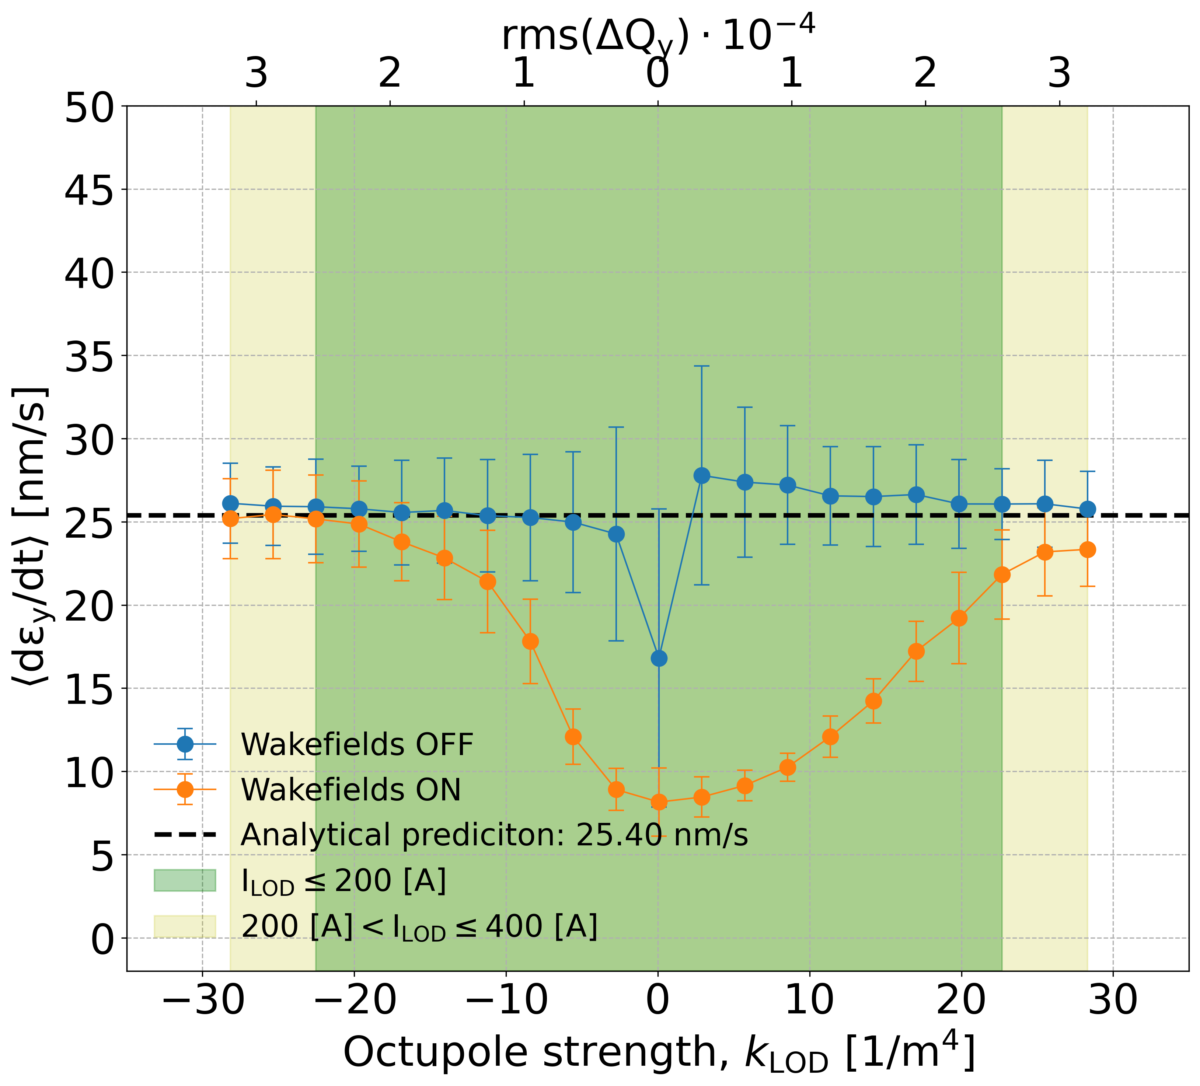
\includegraphics[width=0.8\textwidth]{images/Ch8/deyRates_sps_270GeV_PN1e-8_400MHz_SPS_NewWakesAllcontributions_appendWakes_y-plane_WakesONvsOFF_QpxQpy1_6D_Nb5e5_intensity3e10Scan_vs_TuneSpreadvsExpectedSPS_octupole_current.png}
       \caption{Transvserse emittance growth driven by CC RF phase noise without (blue) and with (orange) the impedance effects. The green and yellow areas indicate regimes where the octupoles require less than 200\,A and 400\,A respectively for their operation.}
       \label{fig:pyheadtail_cc_impedance_2022_md_octupole_current}
\end{figure}

From Fig.~\ref{fig:pyheadtail_cc_impedance_2022_md_octupole_current}, we make the following observations:
\begin{enumerate}
   \item The asymmetry in the suppression factor for positive and negative detuning with amplitude observed in the simulations for the 2018 experimental conditions (Chapter~\ref{Ch:suppression_impedance}) seems to be mitigated here. Nevertheless, in order to exit the suppression region the negative polarity of the octupoles (LOD) should be preferred.
   \item Without powering the octupoles (2018 conditions), $k_\mathrm{LOD}$=0, a suppression of a factor of about 3 is observed.
   \item Even for the strongest octupole strengths, $| k_\mathrm{LOD} |\approx 30 \ \mathrm{/m^4}$, the required current remains below 400\,A. Consequently, no crucial limitations are introduced to the experiment from the octupoles operation.
\end{enumerate}

\textbf{Experimental procedure}\\
The experiment was carried out on 16 May 2022, from 09:15 to 18:40. The steps taken during the experimental study were the following:

\begin{enumerate}
   \item Calibration of the $\CC$ phase offset and voltage measurement.
   \item Measurement of the background growth rate in "coast" mode: CC is switched on but with no additional noise injected in its RF system and the Landau octupoles switched OFF.
   \item Measurement of the emittance growth with the Landau octupoles switched OFF and for four different $\CC$ noise levels as in 2018 (CC Experiment A). For each noise level a new bunch was injected.
   \item Measurement of the emittance growth for a selected noise level and varying octupole strength (CC Experiment B). For each octupole setting a new bunch was injected in the SPS.
\end{enumerate}


The details and the results of the above mentioned steps will be presented in the following subsections.

\subsection{Calibration of CC phase offset and voltage measurement}\label{subsec:cc_calibration_2022}
The first step in the CC experiment in 2022 was to measure the $\CC$ voltage and calibrate the phase offset. It is reminded that in the experimental campaign of 2018, it was found that there was a phase offset between the $\CC$ inspector phase\footnote{Inspector phase is the $\CC$ phase set by the $\CC$ operators.}, $\phi_\mathrm{CC, insp}$, and the phase experience by the beam (see Section~\ref{subsec:cc_phase_offset_2018}). Even though simulation studies showed that for the long bunches used in the $\CC$ experiments the $\CC$ phase has no significant impact on the phase noise induced emittance growth~\cite{wp4_triantafyllou_2020} an automated procedure was developed for identifying and correcting this phase offset for completeness. The same procedure provides the amplitude of the $\CC$ voltage too.

To provide an overview, the calibration was performed by varying the inspector phase of CC1 from -180$^\circ$ to +180$^\circ$ in steps of 30$^\circ$. For each step, the crabbing signal was acquired with the Head-Tail monitor and the $\CC$ voltage signal was reconstructed following the same procedure described in Section~\ref{subsec:CC_voltage_2018_measurement}. For each acquisition, the $\CC$ voltage at the center of the bunch, $t=0$, was plotted as a function of the corresponding inspector phase. The results of the inspector phase scan for $\CC$1 are summarised in Fig.~\ref{fig:Vcc_calibration_md_2022} (blue dots). 
The three-paramter sinusoidal function of Eq.~\eqref{eq:sin_fit_cc} which provides the amplitude, the phase and the vertical offset of the signal ($A, \theta, d$) is used to fit the measured data.

%The results are fitted with the three-paramter sinusoidal function of Eq.~\eqref{eq:sin_fit_cc} which provides the amplitude, the phase and the vertical offset of the signal ($A, \theta, d$).


\begin{figure}[!h] % /eos/user/n/natriant/2022/SPS_MDs_2022/cc_md_16May2022/HT_monitor_phase_CC_offset_calibration
   \centering         
   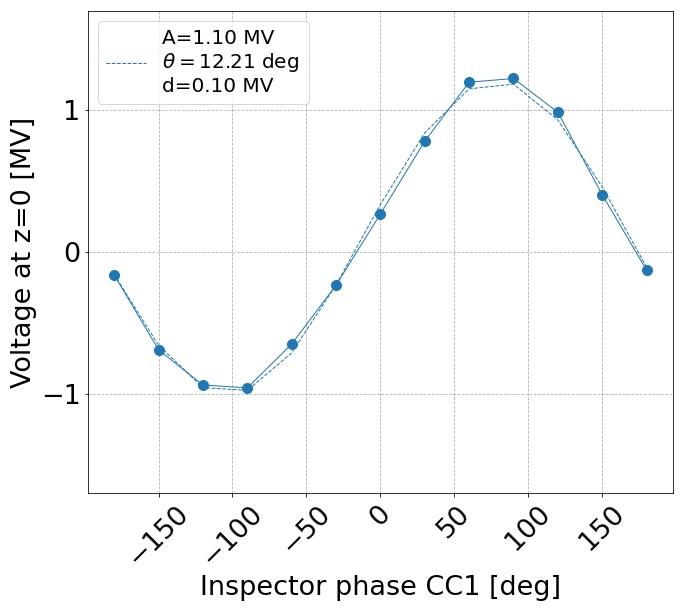
\includegraphics[width=0.7\textwidth]{images/Ch8/Vcc_at_z_zero_vs_inspector_phase_CC1_for_thesis.png}
       \caption{Calibration plot for the CC1 as obtained during the experiment on 16 May 2022, displaying the CC voltage at the center of the cavity $t=0$ for different values of the inspector phase.}
       \label{fig:Vcc_calibration_md_2022}
\end{figure}

The results of the sinusoidal fit (blue dashed line) are illustrated in the legend box in Fig.~\ref{fig:Vcc_calibration_md_2022}. Hence, it can be concluded that from the beam based measurements with the Head-Tail monitor the phase offset was found to be 12.21$^\circ$. For the rest of the experiment, the inspector phase was set to the opposite of the phase offset so that the CC phase is zero. 

From the fit the amplitude voltage of CC1 was found to be (following the discussion in Section~\ref{subsec:CC_voltage_2018_measurement}): $\CCvoltage=A \pm d = 1.1 \pm 0.1$\,MV, very close to the targeted one (1\,MV). This approach of measuring the $\CC$ voltage experienced by the beam is preferred over the approach used in 2018, since now multiple Head-Tail acquisitions are taken into account in contrary with the single acquisition used in 2018.


%since now the amplitude is obtained from a sinusoidal fit over multiple Head-Tail acquisitions while in 2018, only one acquisition was used.


For reference, the calibration for $\CC$1 took place at 270\,GeV and it lasted for about 15 minutes (start: $\sim$09:40, end: $\sim$09:52).


Between $\sim$11:39 and $\sim$11:45 the same scan for CC2 was attempted. However, the cavity tripped systematically due to issues associated with the change of the RF phase. Fixing this issue would have been time-consuming, and was not possible due to the very limited machine time of the MD. Therefore, for the measurements in 2022 $\CC$1 was used.
% CC2 tripped: see the entry of the logbook 4/5/2022, at 11:30:30 

\subsection{Measurement of background growth rate in "coast" mode}\label{subsec:measured_background_growth_cc_md_2022}
After the calibration of CC1, the coast at 270\,GeV was set up for the emittance growth measurements. First, the background emittance growth, with no additional noise injected in the CC and the Landau octupoles switched off was measured. The background emittance growth was found to be similar in both transverse planes: $d\epsilon_x /dt$ = 0.81\,$\mathrm{\mu m}$ and $d\epsilon_y /dt$ = 0.84\,$\mathrm{\mu m}$ in the horizontal and vertical planes respectively. This measured background emittance growth is illustrated in Fig~\ref{fig:cc_md_2022_background_growth_in_scan} for both the horizontal (blue) and vertical (red) planes.

\begin{figure}[!h] % /eos/user/n/natriant/2022/SPS_MDs_2022/cc_md_16May2022/roundA_online_analysis_ws/online_analysis_scripts_figures/coast1
   \centering         
   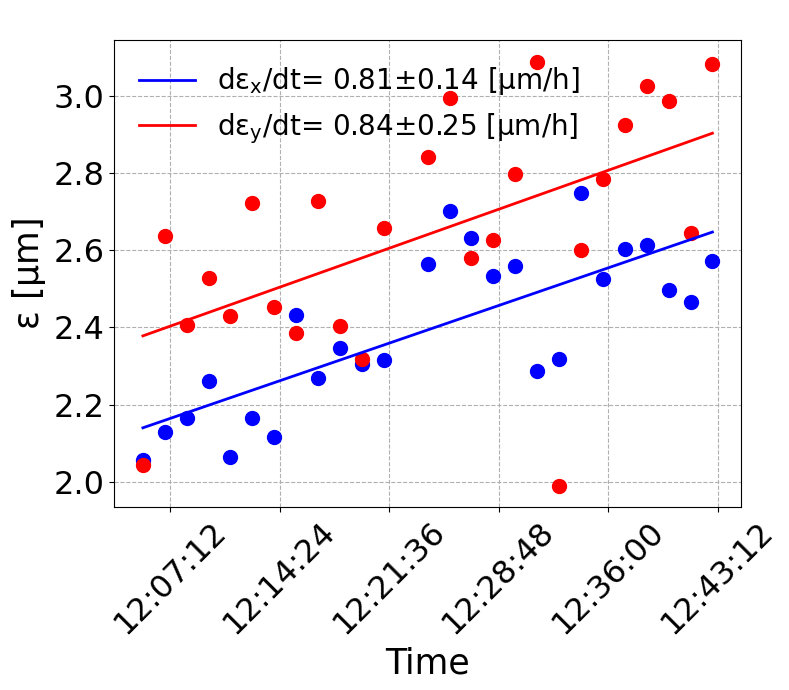
\includegraphics[width=0.7\textwidth]{images/Ch8/cc_md_2022_background_in_scan.png}
       \caption{Horizontal (blue) and vertical (red) background emittance growth measured during the experiment with CC1 in 2022, with no injected artificial noise and with the Landau octupoles switched OFF.}
       \label{fig:cc_md_2022_background_growth_in_scan}
\end{figure}
% There was no valid reason to exclude any of the points even the outliers.

The applications used in the control room for the monitoring of the SPS machine have undergone an upgrade between the years 2018 and 2022. The latest applications which activate the wire scanners and automatically compute the emittance values from the profiles do not compute the respective errors. Nevertheless, the profile measurement data are available and thus the uncertainties of the emittance values can be calculated at a later post-processing stage. This post-processing showed that the uncertainties of the emittance values (computed as shown in Chapter~\ref{Ch:2018_analyisis}) are 2-3 orders of magnitude smaller than the emittance values themselves \footnote{See Appendix~\ref{sec:sps_transverse_beam_profiles}}. Therefore, their impact is insignificant and the uncertainties of the emittance growth rates are dominated by the fluctuation of the Wire Scanner acquisitions. To this end, they are not shown in the emittance growth plot nor included in the fit to facilitate the analysis.

From the above figure, it is evident that there is a significant fluctuation in the emittance values in both transverse planes. By looking at the beam profiles, no evidence (e.g. corrupted profiles, abnormal tails, large errors on the gaussian fit results) was found to exclude some of the points. This fluctuation is introduced by the Wire Scanners used for the measurements. As discussed with the experts it appears to be within the limitations of the instrument for these small emittance values. In order to reduce the sensitivity of the linear fit (from which the emittance growth rates are obtained) longer measurements are required (at least 40 minutes). For larger emittance growth rates, or in other words for larger emittance values, the effects of the fluctuations are mitigated.

Finally, for reference, the "natural" amplitude and phase noise of the $\CC$ at 8\,kHz were measured to be -130.2\,dBc/Hz and 125.7\,dBc/Hz respectively. The theoretically~\cite{PhysRevSTAB.18.101001} expected emittance growth from those noise levels was 0.05\,$\mathrm{\mu/h}$ and 0.19\,$\mathrm{\mu/h}$ in the horizontal and vertical planes respectively from both noise types combined.
% y-plane --> AN: 0.045 um/h, PN: 0.14 um/h
% x-plane --> AN: 0.002 um/h, PN: 0.05 um/h
% Directory to compute these rates: /afs/cern.ch/work/n/natriant/public/SPS_MDs_2022/cc_md_16May2022/cmpt_emit_growth_theoretical_model
% Also some of the growth in the horizontal plane is expected by the IBS. How much I do not know yet.
The rest of the observed growth rates, is due to other sources which have not so far been identified. (see discussion in Chapter~\ref{Ch:2018_analyisis}).

\subsection{Results of CC Experiment A: dependence of emittance growth rates on CC noise power}\label{subsec:cc_md_2022_noise_scan}

The objective of the first part of the experiment was to reproduce the dependence of the emittance growth rates on the CC noise power as observed in 2018. Four different levels of artificial noise were injected in the RF system of the $\CC$ as listed in Table~\ref{tab:noise_settings_2022} and the emittance evolution was recorded in "coast" mode every $\sim$1.5 minute. For each noise level, a new bunch was injected so that all measurements took place with the same initial conditions. The duration of each "coast" varied from about 30 minutes for the low noise levels to about 20 minutes for the strong noise. 

For the strong noise, less measurement time is sufficient since the growth rate obtained from the linear fit on the emittance values is less sensitive to the fluctuations in the wire scanner measurements. Additionally, for strong noise, the emittance reaches very quickly very large values, about 8-10\,$\mathrm{\mu m}$, which eventually degrades the quality of the beam.

Figure~\ref{fig:cc_md_2022_overview_plots_noise_scan} illustrates the transverse emittance growth measured in the SPS in 2022 for the four different noise levels injected in the $\CC$ RF system increasing from top left to bottom right. It can be seen, that there is a clear emittance growth in the vertical plane which is faster for stronger noise as expected. A growth in the horizontal emittance is also observed, but this appears to be independent of the growth in the vertical. This is also confirmed in Fig.~\ref{fig:H_V_emit_growth_noise_scan} where the vertical and horizontal growth rates are plotted as a function of the four different phase noise levels. Consequently, even though in the 2018 analysis (see Chapter~\ref{Ch:2018_analyisis}) the total emittance growth given by $d\epsilon_y/dt +d\epsilon_x/dt $ was considered (in order to account for effects of betatron coupling), in the following analysis of the 2022 experimental data the growth in the horizontal and vertical planes will be treated separately.


% Note 1, figures: /eos/user/n/natriant/2022/SPS_MDs_2022/cc_md_16May2022/roundA_online_analysis_ws/for_thesis
% Note 2, scripts to plot: /afs/cern.ch/work/n/natriant/public/SPS_MDs_2022/cc_md_16May2022/ws_measurements 
\begin{figure}[htp]
   \centering
   \begin{subfigure}{.45\textwidth}
       \centering
       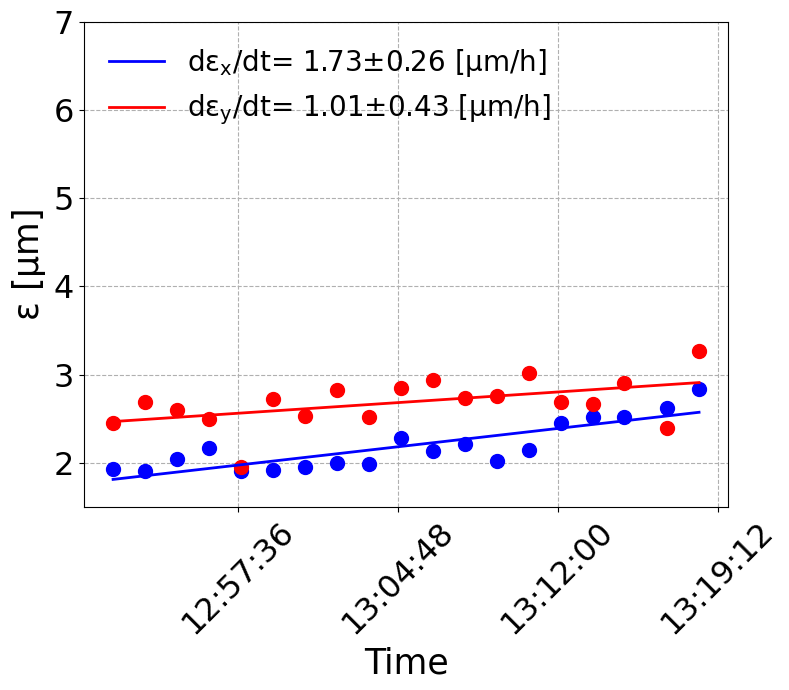
\includegraphics[width=.95\linewidth]{images/Ch8/emit_vs_time_Set1_coast2.png}  
       \caption{-115.2\,dBc/Hz}
       \label{fig:cc_md_2022_coast2}
   \end{subfigure}
   \begin{subfigure}{.45\textwidth}
       \centering
       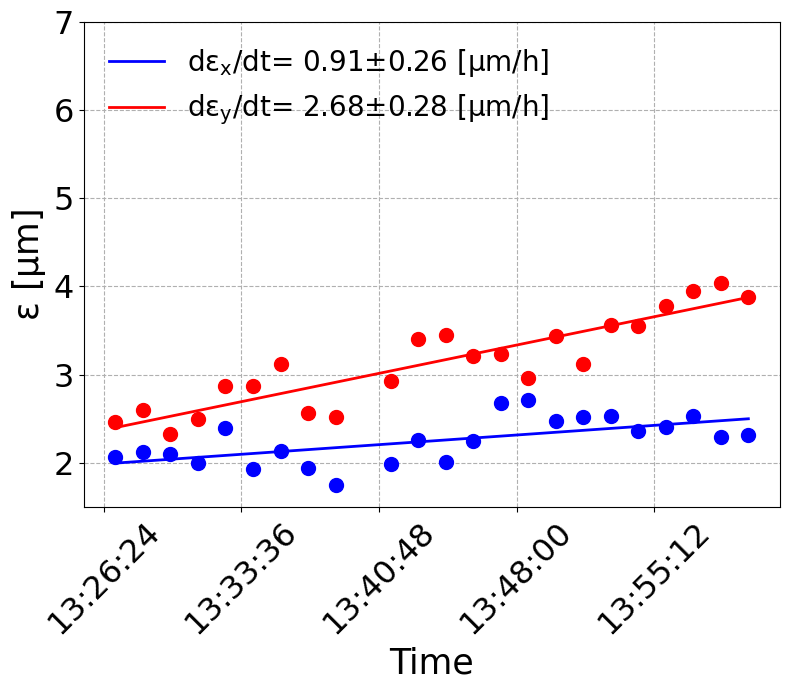
\includegraphics[width=.95\linewidth]{images/Ch8/emit_vs_time_Set1_coast3.png}  
       \caption{-109.5\,dBc/Hz}
       \label{fig:cc_md_2022_coast3}
   \end{subfigure}
   \begin{subfigure}{.45\textwidth}
       \centering
       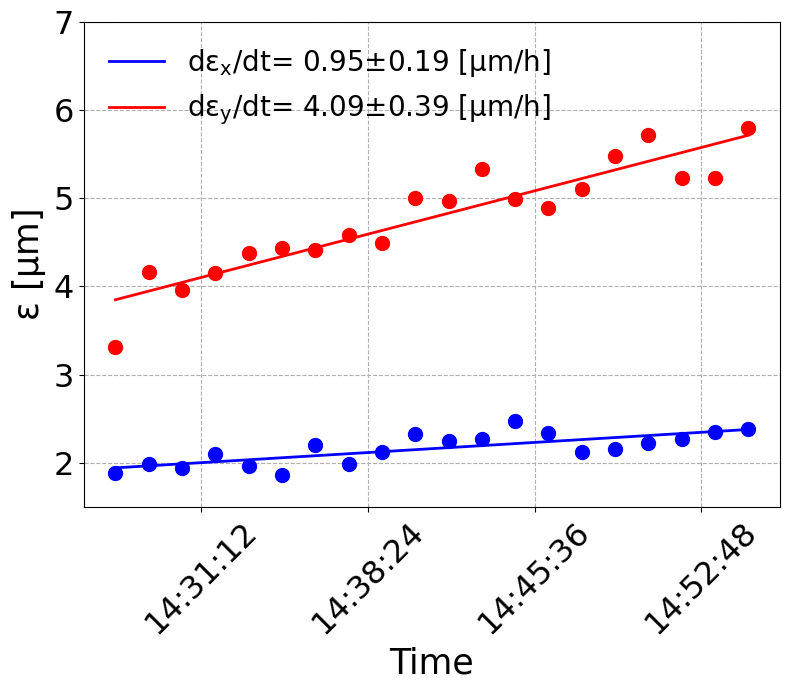
\includegraphics[width=.95\linewidth]{images/Ch8/emit_vs_time_Set1_coast4.png}  
       \caption{-104.7\,dBc/Hz}
       \label{fig:cc_md_2022_coast4}
   \end{subfigure}
   \begin{subfigure}{.45\textwidth}
           \centering
           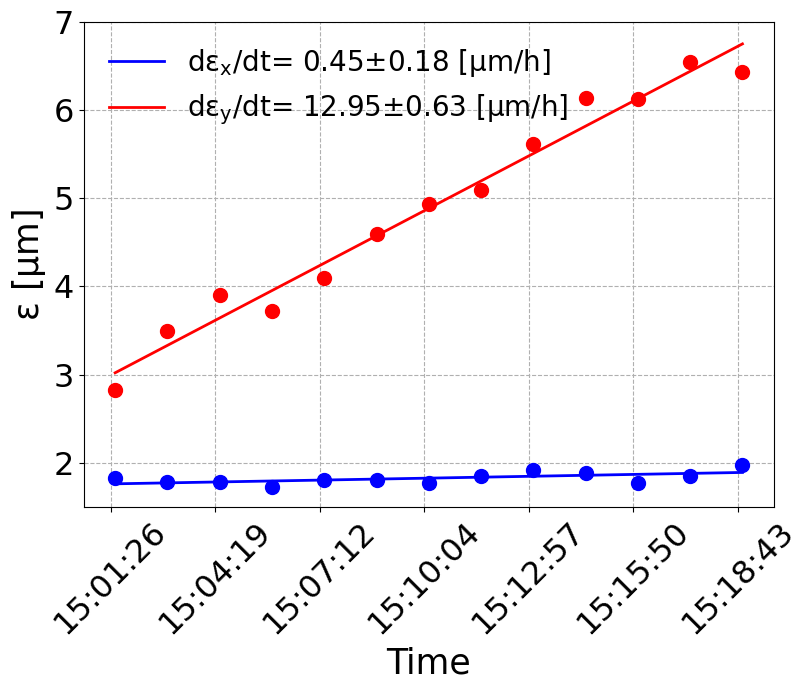
\includegraphics[width=.95\linewidth]{images/Ch8/emit_vs_time_Set1_coast5.png}  
           \caption{-100.1\,dBc/Hz}
           \label{fig:cc_md_2022_coast5}
   \end{subfigure}
   \caption{Horizontal (blue) and vertical (red) emittance evolution of a single bunch during the CC experiment on 16 May, 2022. The different phase noise levels injected in the RF system of CC1, are shown in the caption for each plot.}
   \label{fig:cc_md_2022_overview_plots_noise_scan}
\end{figure}

% Figure: /eos/user/n/natriant/2022/SPS_MDs_2022/cc_md_16May2022/roundA_online_analysis_ws/summary_plots/for_thesis/emit_H_and_V_noise_scan.png
\begin{figure}[!h] 
     \centering         
   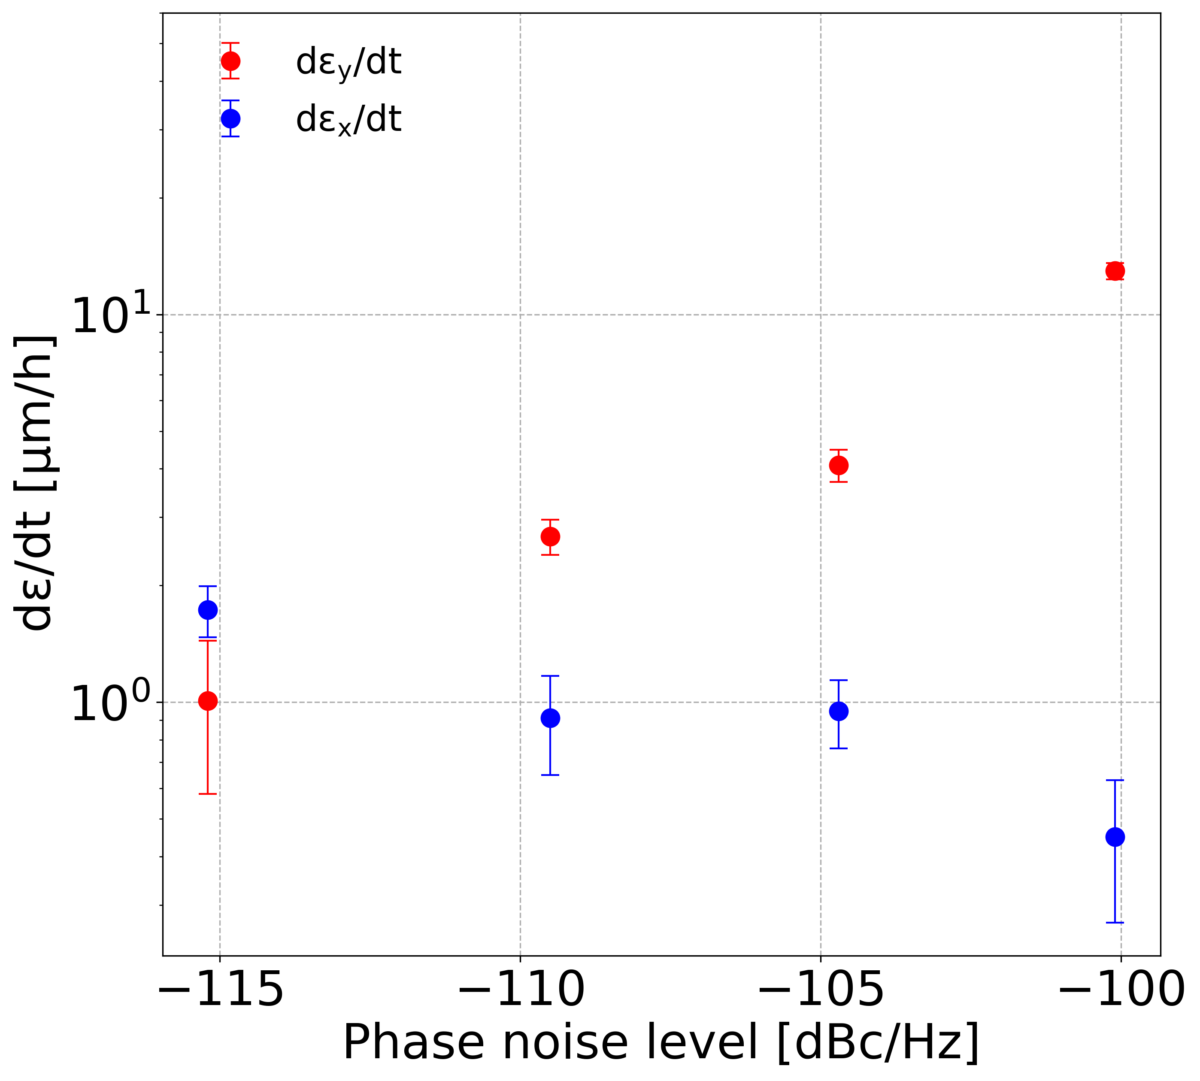
\includegraphics[width=0.7\textwidth]{images/Ch8/emit_H_and_V_noise_scan.png}
       \caption{Overview plot of the emittance growth study with noise injected in the CC1 in 2022. The measured horizontal (blue) and vertical (red) emittance growth rates are shown as a function of the different power levels of applied phase noise. The error bars indicate the error of the linear fit to the emittance values (see Section~\ref{sec:emit_growth_meas_2018}).}
       \label{fig:H_V_emit_growth_noise_scan}
\end{figure}


%\textbf{Summary plot}\\
Figure~\ref{fig:V_emit_growth_background_subtracted_noise_scan} compares the measured (red) and the theoretically calculated (black) vertical emittance growth rates for the different phase noise levels. For the comparison the background growth rate measured in the vertical plane (see Section~\ref{subsec:measured_background_growth_cc_md_2022}) of 0.84\,$\mathrm{\mu m /h}$ is subtracted from the measured values. The theoretically calculated values are obtained by inserting the phase noise levels of Table~\ref{tab:noise_settings_2022} in Eq.~\eqref{eq:dey_pn} for bunch length of $4 \sigma_t$ = 1.83\,ns, energy of 270\,GeV and the vertical beta function at the location of CC1, 76.07\,m . The subtraction of the background has practically no impact on the high noise levels but it is significant for the small ones.

% Figure: /eos/user/n/natriant/2022/SPS_MDs_2022/cc_md_16May2022/roundA_online_analysis_ws/summary_plots/for_thesis/emit_V_background_subtracted_noise_scan.png
\begin{figure}[!h]
   \centering         
   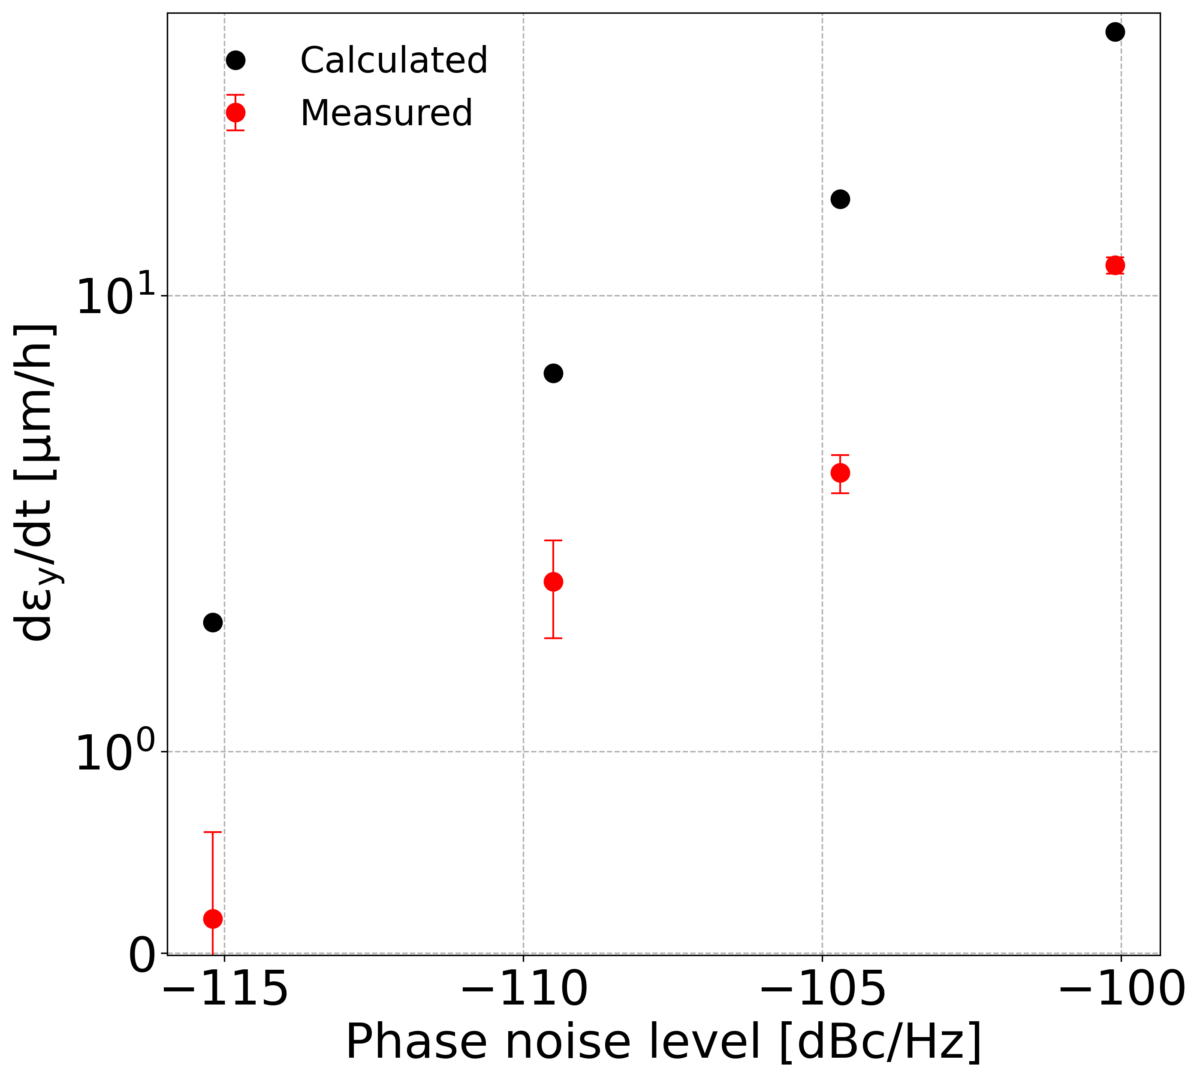
\includegraphics[width=0.7\textwidth]{images/Ch8/emit_V_background_subtracted_noise_scan.png}
       \caption{Summary plot of the emittance growth study with different noise levels injected in the RF system of CC1 in 2022. The vertical measured growth rate (red) and the expected growths from the theoretical model~\cite{PhysRevSTAB.18.101001} (black) are shown as a function of the different levels of applied phase noise. The error bars indicate the error of the linear fit on the emittance values (see Section~\ref{sec:emit_growth_meas_2018})}
       \label{fig:V_emit_growth_background_subtracted_noise_scan}
\end{figure}

From Fig.~\ref{fig:V_emit_growth_background_subtracted_noise_scan} it becomes evident that the measured emittance growth rate increases for higher noise levels as expected. Furthermore, it is observed that the theory systematically overestimates the growth rates. The averaged discrepancy over all noise levels, but the first one, is a factor 4: numerical values are given in Table~\ref{tab:cc_md_2022_noise_scaling}. In the computation of the average, the growth rates for the first noise level are not taken into account since the uncertainty of the corresponding measured growth is very big ($\sim 50\%$ of the emittance value itself).

\begin{table}[!hbt]
	\centering
   \caption{Comparison between the measured and the calculated transverse emittance growth rates for the different phase noise levels during the CC experiment of 2022. The analytical emittance growth rates were computed using Eq.~\eqref{eq:dey_pn} for bunch length of $4\sigma_t$=1.83\,ns.}
	\begin{tabu} to \textwidth { X[c,m] X[c,m] X[c,m] }
		&& \\[-6mm]
		\toprule \toprule
		\multicolumn{1}{c}{$\mathbf{10\,\boldsymbol{\log}_{10} \mathcal{L}(f)}$} &
      \multicolumn{2}{c}{\textbf{Growth rate [}$\mathbf{\boldsymbol{\mu}}$\textbf{m/h]}}  \\
		%\bottomrule
      \multicolumn{1}{c}{\textbf{[dBc/Hz]}} & \multicolumn{1}{c}{\textbf{\textbf{Measured}}} & \multicolumn{1}{c}{\textbf{Calculated}}  \\
      \midrule
      \multicolumn{1}{c}{-115.2}  & \multicolumn{1}{c}{0.17} & \multicolumn{1}{c}{1.64} \\
      
      \multicolumn{1}{c}{-109.5}  & \multicolumn{1}{c}{1.84} & \multicolumn{1}{c}{6.11} \\

      \multicolumn{1}{c}{-104.7}  & \multicolumn{1}{c}{3.25} & \multicolumn{1}{c}{18.44}  \\

      \multicolumn{1}{c}{-100.1}  & \multicolumn{1}{c}{12.11} & \multicolumn{1}{c}{53.19}  \\ 
      \arrayrulecolor{black}\bottomrule
	\end{tabu}
   \label{tab:cc_md_2022_noise_scaling}
\end{table}

The results from $\CC$ Experiment A showed that:
\begin{itemize}
   \item The measured emittance growth was found to scale with the noise power as expected from the theory. 
   \item The measured growth rates were found to be systematically lower than the analytically expected values. This observation is in accordance with the experimental observations of the 2018 campaign and validates the reproducibility of the experiment. 
   \item The discrepancy between measured and theoretically expected values was found to be about a factor of 4, which is very close to the suppression factor of 3 which is expected from the PyHEADTAIL simulations with impedance (see Fig.~\ref{fig:pyheadtail_cc_impedance_2022_md_octupole_current} for $k_\mathrm{LOD}=0$).
\end{itemize}



\subsection{Results of CC Experiment B: sensitivity of emittance growth rates to amplitude-dependent tune shift}\label{subsec:cc_md_2022_octupole_scan}

The second part of the experiment aimed to validate that the beam coupling impedance suppresses the $\CC$ phase noise-induced emittance growth through the mechanism described in Section~\ref{sec:suppression_mechanism}. The strategy for this proof-of-concept experiment was to measure the emittance growth for one level of phase noise (-104.7\,dBc/Hz or 3.4$\times 10^{11} \ \mathrm{rad^2/Hz}$) but for different octupole settings with the goal of reproducing the behavior shown in Fig.~\ref{fig:pyheadtail_cc_impedance_2022_md_octupole_current}. In the limited time available for the experiment performing the full scan on the octupole settngs was not feasible. Only five octupole strengths could be used, $k_\mathrm{LOD} = \pm 5 \ \mathrm{m^{-4}}, 10 \ \mathrm{m^{-4}}$ and $15 \ \mathrm{m^{-4}}$. The last value of octupole strength is expected to restore the growth rate to almost the values predicted by the theoretical model~\cite{PhysRevSTAB.18.101001} (approximately 20 $\mathrm{\mu m/h}$). For each setting the bunch evolution was recorded for about 20 minutes by acquiring repeated Wire Scanner measurements and then performing a linear fit. For the measurements of each setting a fresh bunch was used so that the initial conditions each time are as close as possible.

The individual measurements of the transverse emittance evolution for each octupole setting are shown in Fig.~\ref{fig:cc_md_2022_overview_plots_klod_scan}. Two main observations can be made. First, there is a clear sensitivity of the measured evolution of the vertical emittance to the octupole strength as expected from the PyHEADTAIL simualtions with the SPS transverse impedance model. The second observation is that a growth of $\sim 2-4 \ \mathrm{\mu m/h}$ is also observed in the horizontal plane. However, it does not seem to depend on the octupole strength. Both observations are also seen in the summary plot of Fig.~\ref{fig:H_V_emit_growth_background_subtracted_octupole_scan}.

% location: /eos/user/n/natriant/2022/SPS_MDs_2022/cc_md_16May2022/roundA_online_analysis_ws/for_thesis
% script to plot: /afs/cern.ch/work/n/natriant/public/SPS_MDs_2022/cc_md_16May2022/ws_measurements 
\begin{figure}[htp]
   \centering
   \begin{subfigure}{.45\textwidth}
       \centering
       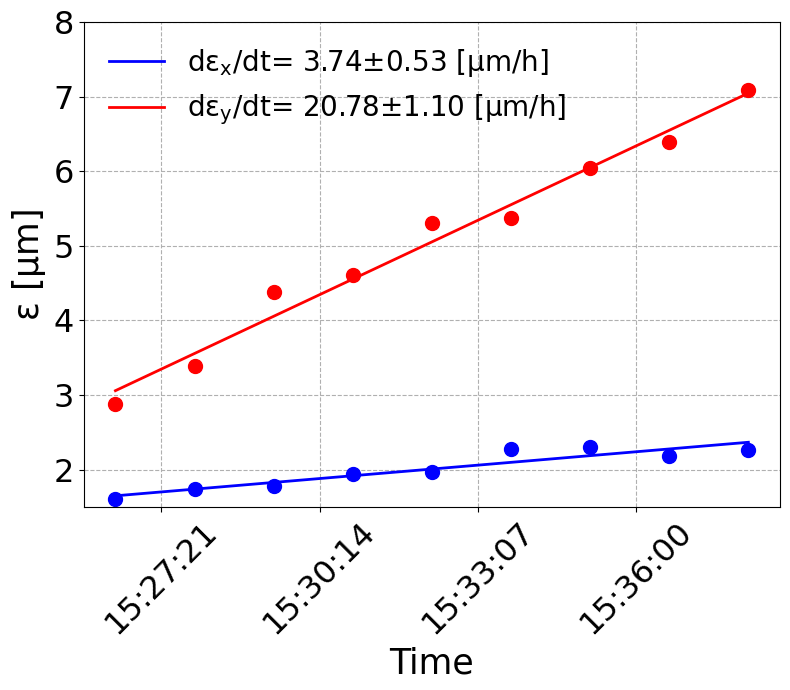
\includegraphics[width=.95\linewidth]{images/Ch8/emit_vs_time_Set1_coast6.png}  
       \caption{$k_\mathrm{LOD}=+15 \ \mathrm{/m^{4}}$}
       \label{fig:cc_md_2022_coast6}
   \end{subfigure}
   \begin{subfigure}{.45\textwidth}
       \centering
       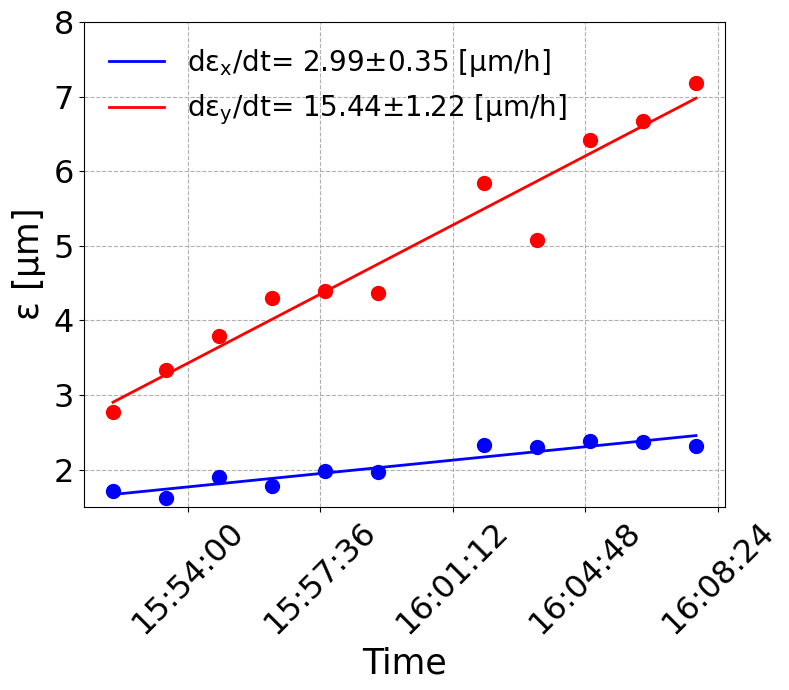
\includegraphics[width=.95\linewidth]{images/Ch8/emit_vs_time_Set1_coast7.png}  
       \caption{$k_\mathrm{LOD}=+10 \ \mathrm{/m^{4}}$}
       \label{fig:cc_md_2022_coast7}
   \end{subfigure}
   \begin{subfigure}{.45\textwidth}
       \centering
       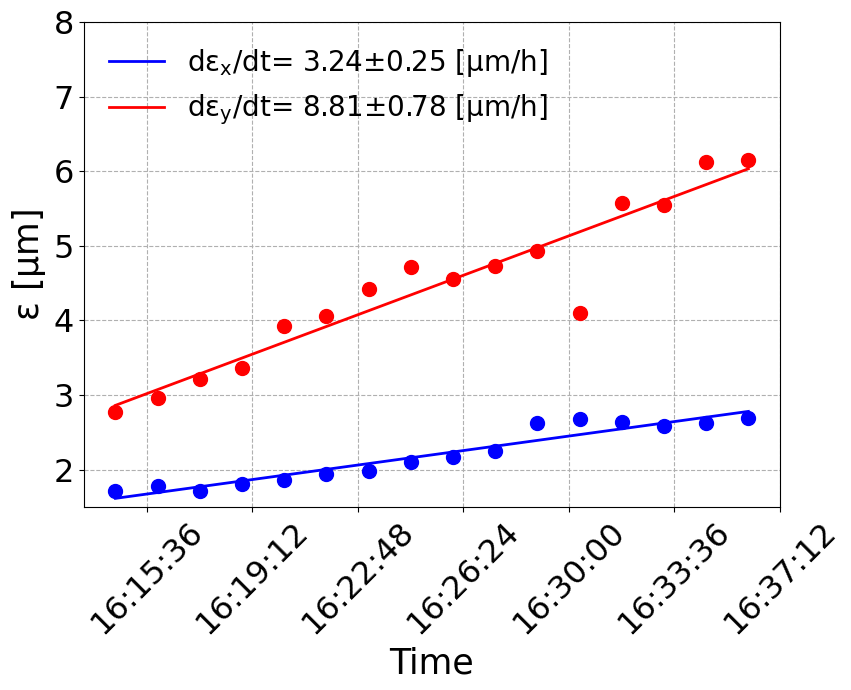
\includegraphics[width=.95\linewidth]{images/Ch8/emit_vs_time_Set1_coast8.png}  
       \caption{$k_\mathrm{LOD}=+5 \ \mathrm{/m^{4}}$}
       \label{fig:cc_md_2022_coast8}
   \end{subfigure}
   \begin{subfigure}{.45\textwidth}
           \centering
           \includegraphics[width=.95\linewidth]{images/Ch8/emit_vs_time_Set1_coast9.png}  
           \caption{$k_\mathrm{LOD}=-5 \ \mathrm{/m^{4}}$}
           \label{fig:cc_md_2022_coast9}
   \end{subfigure}
   \caption{Horizontal (blue) and vertical (red) emittance evolution of a single bunch during the CC experiment on 16 May, 2022 driven by phase noise of -104.7\,dBc/Hz. The different octupole settings are displayed in the captions of each plot.}
   \label{fig:cc_md_2022_overview_plots_klod_scan}
\end{figure}

%\textbf{Unstable bunch for strong negative octupole strength}\\
Following the measurements presented above, there was an attempt to measure the emittance growth for $k_\mathrm{LOD}=-10 \ \mathrm{/m^4}$. However, the bunch was found to be unstable in the horizontal plane which resulted to loss of the beam. The instability was observed in the turn-by turn-data acquired with the base-band tune (BBQ) measurement system of SPS~\cite{Boccardi:1055568}, where the betatron oscillation amplitude appears to grow exponentially within a few seconds. This is illustrated in Fig.~\ref{fig:instability_BBQ_klod-15_4may2022}.

%The instability was first visible in the horizontal beam profiles acquired with the wire scanners, where long tails start to appear in the distribution. This is illustrated in Fig.~\ref{fig:instability_vertical_ws}. The instability was also observed in the turn-by turn-data acquired with the base-band tune (BBQ) measurement system of SPS~\cite{Boccardi:1055568}, where the betatron oscillation amplitude appears to grow exponentially within a few seconds. This is illustrated in Fig.~\ref{fig:instability_BBQ_klod-15_4may2022}.


% Screenshot from MD logbook
%\begin{figure}[!h]
%   \centering         
%   \includegraphics[width=0.7\textwidth]{images/Ch8/instability_41678.V_IN_OUT_ 17_14_31.png}
%       \caption{Example measurement of the vertical profile during the experiment with phase noise of -104.7\,dBc/Hz injected in CC1 and $k_\mathrm{LOD}=-10 \ \mathrm{/m^4}$. Due to the long tails, the Gaussian fit (solid line) does not represent well the measured points (dots connected with the dashed line).}
%       \label{fig:instability_vertical_ws}
%\end{figure}



% Figure: /eos/user/n/natriant/2022/SPS_MDs_2022/cc_md_16May2022/BBQ/figures/2022.05.16.17.49.04.430450.png
% Plotting: /eos/user/n/natriant/2022/SPS_MDs_2022/cc_md_16May2022/BBQ/plotBBQ_for_thesis.py
\begin{figure}[!h]
   \centering         
   \includegraphics[width=0.7\textwidth]{images/Ch8/2022.05.16.17.49.04.430450.png}
       \caption{Example of the evolution of the horizontal oscillation of the bunch centroid during the CC measurements for $k_\mathrm{LOD}=-10 \ \mathrm{/m^4}$. This measurement is acquired with the BBQ instrument~\cite{Boccardi:1055568}.}
       \label{fig:instability_BBQ_klod-15_4may2022}
\end{figure}


The setting of almost zero linear chromaticity is the most likely explanation for this instability. As mentioned in the introduction of this chapter, the linear chromaticity was set to slightly above zero instead of 0.5-1.0 as had been requested due to miscommunication with the SPS operating team. This increased the probability of the chromaticity sliding to small negative values, which for machines like the SPS which operate above transition can result in beam instabilities~\cite{collective_effects_cas_li}.


It is worth commenting, that the instability appeared in the horizontal plane. A possible explanation is that the $k_\mathrm{LOD}$ families used for the experiment the act mainly in the vertical plane. Hence the resulted tune spread was sufficient to stabilise the beam through the mechanism of Landau damping \footnote{Landau damping is a stabilising mechanism that is applied against beam instabilities. It is demonstrated in the transverse planes in the presence of incoherent betatron tune spread. Further details can be found in~\cite{Herr:1982428, Schenk:2665819}, however a further discussion is out of the scope of this thesis.}.

\textbf{Summary plot}\\
Figure~\ref{fig:H_V_emit_growth_background_subtracted_octupole_scan} shows the measured emittance growth rates (in both planes) as functions of octupole strength. The error bars indicate the error of the linear fit on the emittance values during each coast. The background emittance growth observed in the SPS without any noise injected in the CC1 ($d\epsilon_x/dt$ = 0.81\,$\mathrm{\mu m/h}$ and $d\epsilon_y/dt$ = 0.84\,$\mathrm{\mu m/h}$) is subtracted from the measured values. 
%On this ground, it is reasonable to focus the rest of the analyisis in the vertical plane. 

Similarly to the first part of the experiment (see Section~\ref{subsec:cc_md_2022_noise_scan}), the growth in the horizontal plane seems independent of the growth in the vertical. Furthermore, Fig.~\ref{fig:H_V_emit_growth_background_subtracted_octupole_scan} shows a clear dependence of the measured vertical emittance growth rate on the octupole strengths which appears similar to that expected from the simulations. The results from the experiment support the proposed explanation (in terms of the machine impedance) for the damping of the emittance growth from $\CC$ noise.

Additionally, for the measurements with the octupoles turned off, $k_\mathrm{LOD}=0$, the suppression factor is found to be $\sim$ 4-5 which is similar to what is expected from impedance.

The measured vertical emittance growth for the large octupole strength appears already slightly higher than the analytical prediction. This indicates that there is some uncertainty about the level of quantitative agreement: this will be discussed further in the following paragraph which provides a direct comparison of the measured data with the simulation results.

% Plotting script: 2022/SPS_MDs_2022/cc_md_16May2022/roundA_online_analysis_ws/summary_plots/for_thesis/cc_md_octupole_scan_for_thesis.ipynb
\begin{figure}[!h]
   \centering         
   \includegraphics[width=0.7\textwidth]{images/Ch8/emit_H_and_V_octupole_scan_background_growth_subtracted_modified.png}
       \caption{Measured horizontal (blue) and vertical (red) emittance growth driven by phase noise of -104.7\,dBc/Hz injected in the RF system of CC1 for different octupole settings. The growth predicted from the analytical model without taking into account the impedance induced emittance growth suppression is $\sim$ 19\,$\mathrm{\mu m/h}$.}
       \label{fig:H_V_emit_growth_background_subtracted_octupole_scan}
\end{figure}

At this point, it should be highlighted that the degree of complexity of these studies is very high due to several reasons. First, the experiment aims to investigate the interplay of two effects: a) the $\CC$ noise-induced emittance growth and b) its suppression from impedance.  For both effects, the existing knowledge and previous experience are very limited. % for the first effect and non-existent for the second one. 
Second, preparatory studies indicated that these effects are sensitive to many parameters, including the bunch length, bunch intensity, beam energy, $\CC$ noise level, $\CC$ voltage, machine chromaticity, and tune spread. Third, a lot of uncertainties were introduced from the fact that the SPS did not operate in the usual mode. In particular, differences to the usual operational mode included the use of crab cavities, the noise injected in the CC RF system, the operation of SPS in storage ring mode, and the operation of the octupoles at unusually high strengths (requiring high currents in the coils for extended periods). % usually cycling.
Combining these factors, with the very limited machine time for the measurements, the fact that five data points were collected showing a clear dependence of emittance growth rate on octupole strength is significant.

\textbf{Comparison of measurements against PyHEADTAIL simulations with the SPS impedance}\\

Figure~\ref{fig:cc_md_2022_measurement_vs_pyheadtail_simualtion} provides a direct comparison of the vertical emittance growth measurements with the simulation results from PyHEADTAIL including the SPS transverse impedance model (discussed in Fig.~\ref{fig:pyheadtail_cc_impedance_2022_md_octupole_current}). For the comparison, both measured and simulated rates are normalised with the corresponding analytical prediction (using Eq.~\eqref{eq:dey_pn}). 

% Plotting script: /eos/user/n/natriant/pyheadtail_data/final_for_thesis/2022_conditions/CC1/normalised_growth_vs_measurements/job0010b_plot_loadFromPickles_dey_scanOverAyy_NowakesVSwakes-octupoleSettings-Noconstraintaxy_plot_normalised.ipynb
\begin{figure}[!h]
   \centering         
   \includegraphics[width=0.7\textwidth]{images/Ch8/deyRates_sps_270GeV_PN1e-8_400MHz_SPS_NewWakesAllcontributions_appendWakes_y-plane_WakesONvsOFF_QpxQpy1_6D_Nb5e5_intensity3e10Scan_simulations_vs_measurements_magenta_new_legend.png}
       \caption{Measured horizontal (blue) and vertical (red) emittance growth driven by phase noise of -104.7\,dBc/Hz injected in the RF system of CC1 for different octupole settings. The growth predicted from the analytical model without taking into account the impedance induced emittance growth suppression is $\sim$ 19\,$\mathrm{\mu m/h}$.}
       \label{fig:cc_md_2022_measurement_vs_pyheadtail_simualtion}
\end{figure}

It can be seen, that there is a very good qualitative agreement of the measurements with the simulations, supporting the hypothesis that the impedance leads to damping of the emittance growth rates. Regarding the degree of quantitative agreement, there is some uncertainty, as already discussed above. Nevertheless, this is not surprising due to the complex nature of the effects, involving many different parameters, as discussed in the previous paragraph. Further studies, simulations, and measurements will be needed to investigate the quantitative agreement. One of the possible factors that could explain that quantitative agreement is not yet obtained is the contribution from space-charge: this has not yet been studied, but could affect the tune spread. Space charge was not yet taken into account as its contribution is very small for the discussed experimental configurations. Nevertheless, the tune spread values in the regime of the studies are also very small, $10^{-6}-10^{-4}$, which suggests that the space charge might play some role. This can be investigated in simulations even though it is computationally challenging.

%\begin{itemize}
%   \item The contribution from space charge which is not yet studied and it could affect the tune spread values. 
 %  \item The fact that in the experiment the vertical emittances reached significantly larger final emittances than the 2\,$\mathrm{\mu m}$ that were considered in the simulations. Larger emittances mean larger action which eventually leads to a much larger tune spread than it was initially computed for this study. In other words, for the experimental conditions, $k_\mathrm{+15} \ \mathrm{1/m^4}$ the resulting incoherent spectrum might be sufficient for the coherent tune to lie inside it. %Linear, non-linear?
%\end{itemize}

Investigations of space-charge effects may be carried out in the future, but are beyond the scope of the present work.

%As the objective of the experiment and this thesis, in general, are already achieved, these studies are considered complementary. Therefore, they are not performed yet nor they will be presented here, due to time restrictions for the completion of this thesis. 

%\subsection{Conclusions and outlook}\label{subsec:conlusions_ch8_cc_md}
%The experimental results of the additional experimental campaign with $\CC$s in SPS that took place on May 16, the year 2022 were presented in this section. The subject of the studies was the investigation of the $\CC$ noise-induced emittance growth and in particular its suppression from the beam transverse impedance. The two main objectives were a) to reproduce the scaling of the emittance growth with noise power that was observed in 2018, and b) to confirm that the beam coupling impedance can effectively suppress the $\CC$ phase noise-induced emittance growth. For the latter, the strategy was to reproduce the strong dependence of the suppression factor on the amplitude-dependent tune shift as obtained from PyHEADTAIL simulations with the SPS impedance model.

%Despite the limited available machine time and the numerous uncertainties introduced by the SPS operation outside of its usual mode, the experiment was proved successful. In particular, the experiment demonstrated that the vertical emittance increased for stronger noise in agreement with the observables of 2018 and the expectations from the available analytical model of T.~Mastoridis and P.~Baudrenghien. Moreover, the measurements showed good qualitative agreement with the expected impact of impedance and amplitude detuning: they represent a proof of concept for the mechanism of emittance growth suppression from the transverse impedance. Further studies, simulations (e.g. contribution of space charge), and measurements (e.g. varying octupole strengths over a larger range, impact of linear chromaticity, and the sensitivity to transverse instabilities), will be needed to refine the experimental observations and to investigate the quantitative agreement. 




\section{Experiment with dipole noise}\label{sec:coast_md_damper_2022}
% Presentation with the results:  https://docs.google.com/presentation/d/1C-3FPNUrUUiOFol2bdMlTqf1ZlGVamcZXjf-b4lYlUM/edit#slide=id.g1301694a1dd_0_139
The second proof-of-concept experiment to investigate the damping mechanism from the transverse impedance was conducted the night after the $\CC$ experiments described in the previous section. The emittance growth was induced by the beam damper acting as a pure dipolar noise source. This simplified the experimental procedure for two main reasons. First, there were no limitations and uncertainties introduced by the $\CC$ operation. Secondly, activating the beam damper does not require the teams which operate the $\CC$s and inject artificial noise into their RF system and thus simplifies the organisation. This mitigates the restrictions on finding an available slot for this experiment which eventually was squeezed during the night shift after the measurements with $\CC$s. % cryo team not needed

The strength of the damper kick was not calibrated and therefore the analytical expected emittance growth could not be computed. Nevertheless, the objective was to reproduce the strong dependence on the amplitude detuning which was presented in Fig.~\ref{fig:study_5_dipole_noise}. To this end, the same procedure as for the second part of the $\CC$ experiment was followed: the emittance growth was measured in "coast" mode for constant strength of the noise excitation in the vertical plane but for different octupole settings. The beam and machine parameters are summarised in Table~\ref{tab:machine_beam_param_2022}. The only update was that the linear chromaticity was corrected to $Q^\prime_{x,y}$ = 1.3 in both transverse planes to avoid instabilities due to possible shift of chromaticity to negative values (see Figs.~\ref{fig:instability_BBQ_klod-15_4may2022}).% and~\ref{fig:instability_vertical_ws}). 

The experiment lasted from about 23:50 on the May 16, 2022, until about 04:00 on the May 17, 2022. Even though the available machine time was $\sim$4 hours, only seven octupole strengths could be tested: $+25, +15, +10, +5, 0, -15, -7.5 \ \mathrm{/m^4}$. The reason is that one of the SPS quadrupole magnets tripped around 01:00 disabling the option for operation in "coast" mode, till around 03:00 when the quadrupole magnet could once more be operated.

For each octupole setting, the bunch evolution was recorded for about 10 minutes by acquiring repeated measurements with the Wire Scanners (the same instruments were used for the $\CC$ experiment earlier that day). The short duration of the measurements was a result of the strong noise excitation which resulted in a clear linear growth of the vertical emittance which quickly reached large values. This can be seen in the individual measurements of the transverse emittance evolution for each octupole setting which are presented in the Appendix... For the measurements of each setting a fresh bunch was injected. 


\textbf{Summary plot}\\
% no bacgkorund growth is subtracted here. It was not measured. Sensitivity very small as we are dealing with very strong emittance growth. Impact of backgorund growth is insignificant.
The experimental results are summarised in Fig.~\ref{fig:coast_dipole_noise_damper_md_2022_measurement}. The measured horizontal and vertical emittance growth are plotted as a function of the different octupole strengths with blue and red colors respectively. The error bars indicate the error of the linear fit on the emittance values during each coast. The background emittance growth without any noise excitation from the damper was not measured and thus is not subtracted from the displayed values. However, the impact of the background growth (usually measured to be between 0.5-1$\mathrm{\mu m/h}$ in both transverse planes) is insignificant for the emittance growth rates of this study ($ > 10 \ \mathrm{\mu m/m}$).
 

The emittance growth observed in the horizontal plane appears to be independent of the octupole strengths, agreeing with the observations during the $\CC$ experiment (see Section~\ref{sec:cc_md_2022}). 

In the vertical plane, there is a clear dependence of the measured emittance growth on the strength of the octupoles as expected (see Fig.~\ref{fig:study_5_dipole_noise}). The results of the experiment thus further support the hypothesis that the suppression of emittance growth observed from $\CC$ noise is a consequence of the machine impedance. However, it is not clear if the used octupole strength was sufficient to be beyond the suppression region. More data points with higher octupole strength would be needed to confirm whether this was the case, and further experiments to investigate the limits in more detail are planned. This is planned to be tested in dedicated future experiments.

Finally, it is worth commenting that, unlike the $\CC$ experiment that was conducted earlier that day, no vertical instability was observed in this experiment. It appears, that correcting to $Q^\prime_{x,y}$ = 1.3 was an effective way of avoiding it.
  

% Plotting script: /eos/user/n/natriant/2022/SPS_MDs_2022/coast_md_damper_16May2022/summary_plots/create_pickle_for_octupole_scan.ipynb
\begin{figure}[!h]
   \centering         
   \includegraphics[width=0.7\textwidth]{images/Ch8/emitGrowth_H_V_dipole_noise_damper_md_measurements.png}
       \caption{Measured horizontal (blue) and vertical (red) emittance growth driven by dipole noise introduced with the SPS beam kicker in the vertical plane for different octupole settings.}
       \label{fig:coast_dipole_noise_damper_md_2022_measurement}
\end{figure}

\textbf{Underlying theory}\\
It is worth mentioning that the simulation studies and experimental results (from 2018 and 2022) presented in this thesis, motivated the development of a theoretical description for the suppression of the noise-induced emittance growth from the beam transverse impedance. The theory was recently developed by the colleague X.~Buffat~\cite{Buffat:2022dac, van_kamper_presentation_xavier_theory}. 

The theory developed is a simplification of the approach of Y.~Alexahin (in the context of beam-beam interactions)~\cite{Alexahin:485304}. In particular, X.~Buffat, using the Van Kampen mode approach~\cite{VANKAMPEN1955949}, adapted Y.~Alexahin's approach for configurations featuring linear detuning and a complex tune shift from a collective force. 

% This paragraph is modified from the conclusions in Xavier's paper.%
It was shown that the emittance growth driven by an external noise source can be significantly reduced by a collective force. To observe the suppression a damping force is necessary. The suppression is enhanced in configurations where the real tune shift is larger than the spread of the betatron frequencies i.e.~the coherent mode emerges from the incoherent spectrum~\cite{Buffat:2022dac}.

This theory supports the studies presented in this thesis. It also explains the asymmetry in the dependence of the emittance growth suppression for positive and negative detuning coefficients observed in PyHEADTAIL simulations (see Chapter~\ref{Ch:suppression_impedance}). Moreover, it was used to fit the experimental data measured during the experiment with dipole noise with very promising results.
% The figures is a screenshot from the plots of the following presentation: https://indico.cern.ch/event/1170242/contributions/4915101/attachments/2476586/4250387/2022-07-07_crabMD-expanded.pdf
%\begin{figure}[!h]
%   \centering         
%   \includegraphics[width=0.6\textwidth]{images/Ch8/fit_van_kamper_damper_md_data_xavier.png}
%       \caption{Fit of Eq... to the measured emittance growth rates (points) during the experiment with a dipolar noise source. This figure is a courtesy of X.~Buffat.}
%       \label{fig:fit_van_kamper_xavier}
%\end{figure}


%\subsection{extra}
%check the  detuning with amplitude
%https://docs.google.com/presentation/d/1yaGKJ20O-jVg0R3bdj62l5VzltwjBBHtphKq5HI9xrY/edit#slide=id.g104dd3ff735_0_184


%\section{Bunch length measurements} --> Moved in the appendix
% https://docs.google.com/presentation/d/1cqXVwsXoorYqU9Td0qiFDBcyAn9XrNLmL_kvYOj61yU/edit#slide=id.g129fd6f84c7_1_5


\section{Conclusions and outlook}\label{sec:Ch8_conclusions}
%The experimental results of the additional experimental campaign with $\CC$s in SPS that took place on May 16, the year 2022 were presented in this section. 
In this chapter, we have summarised the results of the experiments of 16 May 2022 to investigate emittance growth in SPS driven by CC phase and amplitude noise.  The main aim was to determine whether suppression of the growth rates might result from the machine impedance. The two specific objectives were a) to reproduce the scaling of the emittance growth with noise power that was observed in 2018, and b) to confirm that the beam coupling impedance can effectively suppress the $\CC$ phase noise-induced emittance growth. For the latter, the strategy was to reproduce the strong dependence of the suppression factor on the amplitude-dependent tune shift as obtained from PyHEADTAIL simulations with the SPS impedance model.

Despite the limited available machine time and the numerous uncertainties resulting from operation of the SPS outside of the usual mode, the experiment yielded useful data.. In particular, the experiment demonstrated that the vertical emittance increased for stronger noise in agreement with the observables of 2018 and the expectations from the available analytical model of T.~Mastoridis and P.~Baudrenghien. Moreover, the measurements showed good qualitative agreement with the expected impact of impedance and amplitude detuning: they represent a proof of concept for the mechanism of emittance growth suppression from the transverse impedance. Further studies, simulations (e.g.~contribution of space charge), and measurements (e.g.~varying octupole strengths over a larger range, impact of linear chromaticity, and the sensitivity to transverse instabilities), will be needed to refine the experimental observations and to investigate the quantitative agreement. 

Finally, additional measurements with emittance growth driven by a pure dipolar noise source (the beam transverse damper) clearly demonstrated the dependence of the emittance growth suppression on the amplitude-dependent tune shift.  This further supports the conclusions from the experiments using the $\CC$, regarding the hypothesis that suppression of the emittance growth can result from the machine impedance.

% From IPAC
%During the SPS CC tests in 2018, it was found that theoretical calculations of the transverse emittance growth from CC RF noise overestimated the measurements by a factor 4 (Chapter~\ref{Ch:2018_analyisis}). Simulations with PyHEADTAIL indicated that the discrepancy might be explained by impedance effects, in particular when the coherent tune is shifted outside of the incoherent spectrum (Chapter~\ref{Ch:suppression_impedance}). The simulations also indicated that the suppression is related to the dipole motion (mode 0) and a strong dependence on amplitude detuning: this was tested experimentally in the SPS in 2022. 

%The emittance growth studies took place first in the presence of $\CC$ RF phase noise and after in the presence of pure dipolar noise excitation from the beam transverse damper. The results from both expereiments show good qualitative agreement with the expected impact of impedance and amplitude detuning: they represent a proof of concept for the mechanism of emittance growth suppression from transverse impedance. 


%The noise kicks from the transverse damper were not calibrated so a quantitative comparison with the simualtion results was not feasible. For the experiment where the emittance growth was driven by $\CC$ the quantitative agreement was 


%The objective of the experimental campaign with emittance growth studies se in the SPS in 2022 was to validate experimentally the $\CC$ RF noise induced emittance growth suppression mechanism from the beam transverse impedance as suggested by PyHEADTAIL simualtions. The simualtions suggested that the meachanism is related to the dipole motion (mode 0) to this end two experiments took place. In the first, the emittance growth was driven by $\CC$ RF phase noise (like in 2018), while in the second it was driven by the beam transverse noise which provided a pure dipolar noise excitation.

%This would a) explain the 

%IPAC?



\chapter{Application and impact for HL-LHC}
% This first paragraph is slightly modified from the phd description: /eos/user/n/natriant/Documents/education/cern/doctoral/DOCT_PhD v2.docx
\thispagestyle{simple} % formatting the first page of each chapter

The work presented in this thesis addressed the emittance growth driven by noise in the $\CC$ RF system, which is anticipated to limit the performance of the HL-LHC. The validity of the Mastoridis--Baudrenghien model, which predicts the $\CC$ RF noise-induced emittance growth was benchmarked against experimental data and its limitations were identified. Based on tracking simulations and experimental measurements it was shown that the beam transverse impedance can have a significant impact on the noise-induced emittance growth. 

The studies presented in this thesis were conducted at the CERN SPS, where two prototype $\CC$s were installed in 2018, to allow for tests with proton beams before their installation in the LHC.

The first beam dynamic studies with $\CC$s and proton beams took place in 2018 in the SPS and are presented in this thesis. By analysing the emittance growth measurements it was found that $\CC$ RF noise-induced emittance growth was a factor four on average lower than predicted from the Mastoridis--Baudrenghien model. Follow-up studies excluded the possibility that the observed discrepancy was a result of some error in the analysis of the experimental data.


%The HL-LHC project is the designed uprade of the LHC mahine aiming at about a five-fold increase of the yearly luminosity production with proton beams compared to the present LHC operation. The HL-LHC will employ $\CC$s in the two main experiments (ATLAS and CMS) to restore the luminosity reduction caused by the crossing angle. A particular challenge about the $\CC$s' operation is associated with the fact they are expected to induce undesired transverse emittance growth due to noise in their RF control system, and therefore loss of luminosity. Given the very tight HL-LHC target values for luminosity loss, a solid understanding of the emittance growth due to $\CC$ RF noise is essential. The scope of this thesis has been to understand, characterise, and evaluate the mechanism of the $\CC$ RF noise-induced emittance growth for proton beams through tracking simulations and experimental studies. 

%In 2015, T.~Mastoridis and P.~Baudrenghien developed an analytical model for predicting the emittance growth induced by noise in the $\CC$ RF system which is used for setting the specifications for the noise limits on $\CC$s in HL-LHC. The model was benchmarked with tracking simulations, however, in order to gain confidence in its predictions, benchmarking with experimental measurements was required. 

%Two prototype $\CC$s have been installed in the SPS in 2018, to allow for tests with proton beams prior to their installation in the LHC. Even though the SPS and the LHC are very different machines (discussed in the folllowing section), the objective of the SPS tests was to test the validity of the Mastoridis--Baudrenghien model and identify possibile limitations. During the first experimental campaign with $\CC$s in the SPS in 2018, which is analysed in the thesis, it was found that the measured $\CC$ RF noise-induced emittance was a factor four on average lower than predicted from the available theoretical model of Mastoridis--Baudrenghien~\cite{PhysRevSTAB.18.101001}.  Follow-up studies excluded the possibility that the observed discrepancy was a result of some error in the analysis of the experimental data.



%The studies presented in this thesis, were conducted in the SPS machine where two prototype $\CC$s were installed in 2018, to allow for tests with proton beams prior to their installation in the LHC.


%To extend the physics reach of the main experiments of the Large Hadron Collider (LHC) at CERN, the machine will undergo a major upgrade during the coming years. This upgrade, namely the High-Luminosity LHC (HL-LHC) project, aims at about a five-fold increase of the yearly luminosity production with proton beams compared to the present LHC operation. For these ambitious luminosity goals, the precise control and minimization of beam degradation (such as losses and emittance growth) is critical. A particular challenge is associated with the fact that HL-LHC will employ Crab Cavities to compensate the crossing angle of the colliding bunches, and hence to restore the head-on collisions, in the two main experiments (ATLAS and CMS). However, these Crab Cavities are expected to result in undesired transverse emittance growth due to noise in their RF control system, and therefore loss of luminosity. %  by residual noise on the beam introduced by the crab cavity RF control. 
%Given the very tight HL-LHC target values for luminosity loss and emittance growth from the Crab Cavities (see Introduction chapter) a solid understanding of the emittance growth due to Crab Cavity RF noise is essential. 


%In 2015, T.~Mastoridis and P.~Baudrenghien developed an analytical model for predicting the emittance growth induced by noise in the $\CC$ RF system which is used for setting the specificationsfor the noise limits on $\CC$s in HL-LHC. The model was benchmarked with tracking simulations, however, in order to gain confidence in its predictions, benchmarking with experimental measurements was required. During the first experimental campaign with $\CC$s in the SPS in 2018, it was found that the predictions from the Mastoridis--Baudrenghien model overestimated the measured emittance growth by a factor of four on average. Detailed follow-up studies excluded the possibility that the observed discrepancy was a result of some error in the analysis of the experimental data.

%The HL-LHC will employ $\CC$s in the two main experiments (ATLAS and CMS) to restore the luminosity reduction caused by the crossing angle. A particular challenge about the $\CC$s' operation is associated with the fact they are expected to induce undesired transverse emittance growth due to noise in their RF control system, and therefore loss of luminosity. The scope of this thesis has been to understand, characterise, and evaluate the mechanism of the $\CC$ RF noise-induced emittance growth for proton beams through tracking simulations and experimental studies. A new mechanism of emittance growth suppression resulting from the beam tranvserse impedance was identified.


%Two prototype crab cavities have been installed in the SPS machine and were tested with a proton beam in 2018, prior to the installation in the LHC. A particular challenge about their operation is associated with the fact that the Crab Cavities are expected to induce undesired transverse emittance growth due to noise in their RF control system. This thesis investigated the mechanism of the emittance growth due to Crab Cavity RF noise with tracking simulations and experimental measurements.



%To extend the physics reach of the main experiments of the Large Hadron Collider (LHC) at CERN, the machine will undergo a major upgrade during the coming years. This upgrade, namely the High-Luminosity LHC (HL-LHC) project, aims at about a five-fold increase of the yearly luminosity production with proton beams compared to the present LHC operation. For these ambitious luminosity goals, the precise control and minimization of beam degradation (such as losses and emittance growth) is critical. A particular challenge is associated with the fact that HL-LHC will employ Crab Cavities to compensate the crossing angle of the colliding bunches, and hence to restore the head-on collisions, in the two main experiments (ATLAS and CMS). However, these Crab Cavities are expected to result in undesired transverse emittance growth due to noise in their RF control system, and therefore loss of luminosity. %  by residual noise on the beam introduced by the crab cavity RF control. 
%Given the very tight HL-LHC target values for luminosity loss and emittance growth from the Crab Cavities (see Introduction chapter)
%a solid understanding of the emittance growth due to Crab Cavity RF noise is essential. 

%To study the transverse emittance growth induced in the presence of the Crab Cavities, two prototype Crab Cavities were installed in the SPS in 2018, for experimental tests. The first round of analysis of the experimental studies indicated that the measured emittance growth was a factor 2-3 lower than predicted from the available theoretical model of T.~Mastoridis and P.~Baudrenghien~\cite{PhysRevSTAB.18.101001}. This PhD thesis set out to to understand the results of experimental tests of Crab Cavities in the SPS. Understanding the results is crucial for gaining confidence in the predictions of the theoretical models and the specifications set for the noise limits on Crab Cavities in HL-LHC (which depend on the theoretical model).

%The first step was to revisit thoroughly the experimental data from the SPS tests of 2018 in order to identify any misinterpretations that could explain the observed discrepancy. These studies are presented in Chapter~\ref{Ch:2018_analyisis}. The outcome of this analysis was that the machine configuration and the measurement method could not explain the observed discrepancy. However, these studies provided a clear understanding of the operational aspects of the Crab Cavities in the SPS and of beam-based measurements of the Crab Cavity voltage which were not documented before. Furthermore, an automated procedure for the calibration of the Crab Cavities during operation was established and will be used in future experiments (and was already used in experiments in 2022). Moreover, the quality of the  Gaussian fit on the transverse beam profiles used to obtain the emittance values was verified and the impact of the measurement errors was included in the computation of the emittance growth rates. Open questions, like a possible relation of the transverse emittance growth to the longitudinal beam evolution or the beam intensity, were addressed. Finally, an interesting finding was that the four bunches used in the experiment had different emittance growth rates and only one of them was longitudinally stable. To this end, it was decided that future experimental studies would be performed with a single bunch. Focusing the analysis on the stable bunch the difference between its measured emittance growth rates and the ones predicted from the analytical model was then found to be even larger than had been estimated from the initial analysis at the time of the experiments. Up to a factor of five lower growth rates were observed in the measurements as compared to the theoretical prediction. 

%To study the transverse emittance growth induced in the presence of the Crab Cavities, two prototype Crab Cavities were installed in the SPS in 2018, for experimental tests. The analysis of the experimental data from 2018 indicated that the measured emittance growth was a factor 4 on average lower than predicted from the available theoretical model of Mastoridis--Baudrenghien~\cite{PhysRevSTAB.18.101001}. Detailed follow-up studies excluded the possibility that the observed discrepancy was a result of some error in the analysis of the experimental data.

%Understanding this observation is crucial for gaining confidence in the predictions of the model and the specifications set for the noise limits on Crab Cavities in HL-LHC.% (which depend on the theoretical model).


%The rest of the studies presented in this PhD thesis set out to understand the results of the 2018 experimental tests of Crab Cavities in the SPS. Understanding the results is crucial for gaining confidence in the predictions of the theoretical models and the specifications set for the noise limits on Crab Cavities in HL-LHC (which depend on the theoretical model).


%Chapter~\ref{Ch:2018_analyisis} also provides a thorough examination of the experimental data from the SPS tests of 2018 to identify any misinterpretations that could explain the observed discrepancy. In particular, the quality of the  Gaussian fit on the transverse beam profiles used to obtain the emittance values was verified and the impact of the measurement errors was included in the computation of the emittance growth rates. Open questions, like a possible relation of the transverse emittance growth to the longitudinal beam evolution or the beam intensity, were addressed. The outcome of this analysis was that the machine configuration and the measurement method could not explain the observed discrepancy. However, an interesting finding was that the four bunches used in the experiment had different emittance growth rates and only one of them was longitudinally stable. To this end, it was decided that the investigation of the discrepancy should focus on the experimental data from the first bunch and that future experimental studies would be performed with a single bunch.


% From ipac presentation and conclusions of Chapter 6
%In the following years, 2019-2020, a significant effort with theoretical and simulation studies was made to investigate possible explanations for the discrepancy. These studies are summarised in Chapter~\ref{Ch:investigating_discrepancy}. The sensitivity of the emittance growth rates to possible uncertainties on the measured amplitude of the Crab Cavity voltage and bunch length was tested. Furthermore, the Mastoridis--Baudrenghien theoretical model was benchmarked against different simulation codes, PyHEADTAIL and Sixtracklib, for conditions close to the experimental configuration of 2018. In PyHEADTAIL the emittance growth driven by Crab Cavity RF noise was simulated using a simple representation of the SPS consisting of one transfer map and an interaction point where the noise from the Crab Cavities was modeled as kicks on the angle co-ordinates of the particles. The same studies were repeated with Sixtracklib but the tracking was performed including the detailed optics with the non-linearities of the SPS lattice, the z-dependent orbit shift from the CC kick and the measured noise spectra from the experiments of 2018. It was found that the emittance growth driven by Crab Cavity noise simulated with PyHEADTAIL was in excellent agreement with the Sixtracklib results and with the predictions of the Mastoridis-Baudrenghien theoretical model. It was concluded that there is no sensitivity of the noise-induced emittance growth to the above mentioned parameters.  The use of PyHEADTAIL, for the rest of the studies presented in the thesis, was considered appropriate, since it appears that it includes the necessary beam dynamics for studying this phenomenon.


%It was found that the transverse beam impedance (not included in the Mastoridis--Baudrenghien model) has a significant impact on the transverse emittance growth driven by Crab Cavity RF noise. In particular, PyHEADTAIL simulations using the most updated SPS impedance model demonstrated that the emittance growth is suppressed once the detuning induced by the impedance moves the coherent tune outside of the incoherent tune spectrum. It was also shown that the mechanism of the emittance growth suppression is purely to the rigid or dipole bunch motion (head-tail mode 0) of the beam. For the experimental configuration of the SPS Crab Cavity tests in 2018 it was found that this mechanism results in an emittance growth suppression of about a factor four which is very close to the observed discrepancy . This suggested that the damping effects from the impedance might explain the observed discrepancy between measurements and theoretical predictions.


%n particular, PyHEADTAIL simulations using the most updated SPS impedance model demonstrated that the decoherence and thus the emittance growth is suppressed once the detuning induced by the impedance moves the coherent tune outside of the incoherent tune spectrum. % A similar effect of decoherence suppression was studied in the past in the context of beam-beam modes. 
%It was also shown that the decoherence suppression is related purely to the rigid or dipole bunch motion (head-tail mode 0) of the beam which is excited by the Crab Cavity RF phase noise kicks. For the experimental configuration of the SPS Crab Cavity tests in 2018 it was found that this mechanism results in an emittance growth suppression by a factor up to about 4 which is very close to the observed discrepancy. This suggested that the damping effects from the impedance might explain the discrepancy between the measured and theoretically estimated emittance growth rates. The PyHEADTAIL simulations with the SPS transverse impedance model also revealed that the suppression of the emittance growth as a result of the transverse impedance depends on the amplitude-dependent betatron tune spread. This dependence was tested experimentally in the SPS in 2022.


Tracking simulations with PyHEADTAIL revealed that the transverse beam impedance (not included in the Mastoridis--Baudrenghien model) affects the transverse emittance growth induced by $\CC$ RF noise and may therefore explain the experimental observations. In particular, PyHEADTAIL simulations including the accurate SPS impedance model demonstrated that the noise-induced emittance growth is suppressed by about a factor four for the 2018 experimental conditions. Detailed simulation studies were conducted to characterise this newly observed effect. It was identified that the emittance growth suppression is related purely to the rigid (or dipole) bunch motion (head-tail mode 0) of the beam, which is induced by the $\CC$ RF phase noise. It was also demonstrated that the decoherence and thus the emittance growth is suppressed once the detuning induced by the impedance moves the coherent tune outside of the incoherent tune spectrum. Finally, it was shown that this emittance growth suppression mechanism depends on the amplitude-dependent betatron tune spread and that for large enough tune spread values the emittance growth predicted by the Mastoridis--Baudrenghien model can be restored.


%In particular, simulations with the most updated SPS impedance model demonstrated that the decoherence and thus the emittance growth is suppressed once the detuning induced by the impedance moves the coherent tune outside of the incoherent tune spectrum. The simulations also revealed that the suppression of the emittance growth as a result of the transverse impedance depends on the amplitude-dependent tune shift. Furthermore, it was shown that the emittance growth suppression is related purely to the rigid or dipole bunch motion (head-tail mode 0) of the beam. In the presence of Crab Cavity RF phase noise (which is associated with head-tail mode 0) for the experimental configuration of the SPS Crab Cavity tests in 2018, it was found that the above-described mechanism results in an emittance growth suppression by a factor up to about 4. This is very close to the observed discrepancy and hence suggested that the impedance effects might explain the discrepancy between the measured and theoretically estimated emittance growth rates. %The PyHEADTAIL simulations with the SPS transverse impedance model also revealed that the suppression of the emittance growth as a result of the transverse impedance depends on the amplitude-dependent tune shift. This dependence was tested experimentally in the SPS in 2022.

%It was found that the transverse beam impedance (not included in the Mastoridis--Baudrenghien model nor the simulations so far) has a significant impact on the transverse emittance growth induced by Crab Cavity RF noise. In particular, PyHEADTAIL simulations using the the most updated SPS impedance model demonstrated that the decoherence and thus the emittance growth is suppressed once the detuning induced by the impedance moves the coherent tune outside of the incoherent tune spectrum. A similar effect of decoherence suppression was studied in the past in the context of beam-beam modes. Detailed investigations have shown that the decoherence suppression is related purely to the rigid or dipole bunch motion (head-tail mode 0) of the beam. In the case of Crab Cavity induced noise kicks, this dipolar excitation is provided by the phase noise kicks. For the experimental configuration of the SPS Crab Cavity tests in 2018 it was found that this mechanism results in an emittance growth suppression by a factor up to about 4 which is very close to the observed discrepancy. It is concluded, that this result suggests that the impedance effects might explain the discrepancy between the measured and theoretically estimated emittance growth rates. The PyHEADTAIL simulations with the SPS transverse impedance model also suggested that the suppression of the emittance growth as a result of the transverse impedance depends on the amplitude-dependent tune shift. This dependence was tested experimentally in the SPS in 2022.


An additional campaign took place in the SPS in 2022 and confirmed experimentally for the first time the suggested emittance growth suppression mechanism from impedance induced effects. In particular, the emittance growth driven primarily by $\CC$ RF phase noise was measured as a function of different values of amplitude-dependent betatron tune spread. The measurements were found to be in very good qualitative agreement with the expectations from PyHEADTAIL simulations including the SPS transverse impedance model for very similar machine and beam conditions. Some uncertainty on the quantitative agreement was observed, however, it is within the uncertainties expected from the experimental setup and the instruments used for the measurements. The emittance growth measured in the presence of large betatron tune spread was found to be very close to the predictions of the Mastoridis--Baudrenghien model gaining confidence in its validity.



%was measured as a function of different values of amplitude-dependent betatron tune spread. The experiment yielded results in very good qualitative agreement with the expectations from PyHEADTAIL simulations including the SPS transverse impedance model for very similar machine and beam conditions. Thus, the measurements of 2022 provided a clear experimental validation of the emittance growth suppression mechanism from the beam transverse impedance.



%The main strategy was to measure the emittance growth driven primarily by Crab Cavity RF phase noise as a function of different values of amplitude-dependent betatron tune spread, aiming to reproduce the dependence revealed from the simulations. The experiment yielded results in very good qualitative agreement with the expectations from the PyHEADTAIL simulations including the SPS transverse impedance model for very similar machine and beam conditions.  This result provided a clear experimental validation of the emittance growth suppression mechanism from the beam transverse impedance.  Some uncertainty on the quantitative agreement was observed. However, it is within the uncertainties expected from the experimental setup and the instruments used for the measurements. The emittance growth measured in the presence of large betatron tune spread (which is expected to mitigate the emittance growth suppression mechanism), was found to be very close to the predictions of the Mastoridis--Baudrenghien model gaining confidence in its validity.

%The emittance growth measured in the presence of large betatron tune spread, was found to be very close to the predictions of the Mastoridis--Baudrenghien model (as expected from the simulations), gaining confidence in its validity.

%The measured emittance growth driven by Crab Cavity RF phase noise demonstrated a clear dependence on the amplitude-dependent tune spread which was in very good qualitative agreement with the results from PyHEADTAIL simulations including the SPS transverse impedance model for very similar machine and beam conditions. This result provided a clear experimental validation of the emittance growth suppression mechanism from the beam transverse impedance. Some uncertainty on the quantitative agreement was observed. However, it is within the uncertainties expected from the experimental setup and the instruments used for the measurements, as well as from other effects, like space charge, that are not included in the simulations and might play a role in the overall behavior. The emittance growth measured in the presence of large octupole detuning, was found to be very close to the predictions of the Mastoridis--Baudrenghien model (as expected from the simulations), gaining confidence in its validity.


%Five different experiments were performed with the emittance growth driven by Crab Cavity RF phase noise, pure dipole noise, and Crab Cavity RF amplitude noise. The measurements from all of the experiments support the hypothesis that the impedance provides a damping mechanism. In particular, the measured emittance growth driven by Crab Cavity RF phase noise and a pure dipolar noise source demonstrated a clear dependence on the amplitude-dependent tune spread (introduced by the Landau octupoles in SPS) as expected from PyHEADTAIL simulations including the SPS transverse impedance model. These results confirm the suppression mechanism from the beam transverse impedance and offer an explanation for the experimental observations made in 2018. Furthermore, a direct comparison of the emittance growth rates was made between the results from the experiment with Crab Cavity RF phase noise and PyHEADTAIL simulations for very similar machine and beam conditions. The qualitative agreement demonstrated between experimental data and simulations was very good. Some uncertainty on the quantitative agreement was observed. However, this is within the uncertainties expected from the experimental setup and the instruments used for the measurements, as well as from other effects, like space charge, that are not included in the simulations and might play a role in the overall behavior. The emittance growth measured in the presence of large octupole detuning, was found to be very close to the predictions of Mastoridis--Baudrenghien model (as expected from the simulations), gaining confidence in its validity. Finally, the emittance growth driven by Crab Cavity amplitude noise, which is associated with head-tail mode $\pm$1 and hence is not subject to the emittance growth suppression mechanism, was indeed measured to be very close to the predictions of Mastoridis--Baudrenghien.


%Achieving a good understanding of the 2018 results is essential for developing confidence in the theoretical model and its predictions for the HL-LHC. 
%The results of the experimental measurements with Crab Cavity noise that took place in 2022 are presented in Chapter~\ref{Ch:experimental_CC_2022}. Despite the very limited available machine time, the results demonstrated a clear dependence of the measured emittance growth, driven primarily of Crab Cavity RF phase noise, on the octupole strength, which supports the hypothesis that the impedance provides a damping mechanism, and may offer an explanation for the observations made in 2018.

%impedance and amplitude detuning on emittance growth from Crab Cavity phase noise. The objective was to validate experimentally the suggested suppression mechanism of the emittance growth by the beam transverse impedance, by reproducing the dependence on amplitude-dependent tune spread (introduced by the Landau octupoles) predicted by PyHEADTAIL simulations. 
%Achieving a good understanding of the 2018 results is essential for developing confidence in the theoretical model and its predictions for the HL-LHC. 
%The results of the experimental measurements with Crab Cavity noise that took place in 2022 are presented in Chapter~\ref{Ch:experimental_CC_2022}. Despite the very limited available machine time, the results demonstrated a clear dependence of the measured emittance growth, driven primarily of Crab Cavity RF phase noise, on the octupole strength, which supports the hypothesis that the impedance provides a damping mechanism, and may offer an explanation for the observations made in 2018.

%However, quantitative agreement between theory (taking the impedance into account) and experimental results has not yet been demonstrated. Possible additional factors, such as space charge, have been identified and further studies, including simulations and measurements, are foreseen to investigate the quantitative agreement. An additional experiment in the SPS with emittance growth driven by a pure dipolar source (beam transverse damper), supported the results from the Crab Cavity experiment since it also successfully reproduced the dependence of the suppression on the amplitude-dependent tune shift. This improves the confidence in the current understanding of the experimental results with Crab Cavities.


%To conclude, this thesis presents the first experimental beam dynamic studies with $\CC$s and proton beams. It allowed us to identify in simulations and observe experimentally for the first time the effect of the emittance growth suppression from the beam transverse impedance. The analysis and the results presented here improved the understanding of the $\CC$ RF noise effects that are anticipated in the operation of the HL-LHC.


%it constitutes the first investigation and experimental validation of the suppression mechanism of the Crab Cavity RF phase noise or dipolar noise-induced emittance growth by the beam transverse impedance. The studies provided a significant step forward in the understanding of the mechanism of the transverse emittance growth driven by noise in the Crab Cavity RF systems which directly impacts the HL-LHC performance. This project gained confidence in the validity of the Mastoridis--Baudrenghien model which is used for defining limits on the acceptable noise levels for the HL-LHC Crab Cavities.


%To summarise, this thesis addressed issues of significant importance for HL-LHC as it demonstrates the first experimental beam dynamic studies with Crab Cavities and proton beams. Additionally, it constitutes the first investigation and experimental validation of the suppression mechanism of the Crab Cavity RF phase noise or dipolar noise-induced emittance growth by the beam transverse impedance. The studies provided a significant step forward in the understanding of the mechanism of the transverse emittance growth driven by noise in the Crab Cavity RF systems which directly impacts the HL-LHC performance. The project also confirmed that the relevant beam dynamic effects are sufficiently well understood and that the Mastoridis--Baudrenghien model 




%The identification of the emittance growth suppression from the impedance is a significant step forward in the understanding of the mechanism of the transverse emittance growth driven by noise in the Crab Cavity RF systems which directly impacts the HL-LHC performance.

%The project also provides a strong starting point for future additional studies. Specifically, additional measurements are planned in the SPS to refine the experimental observations, by obtaining more data points showing emittance growth rate as a function of amplitude-dependent tune shift. Furthermore, the interplay of the dipolar noise or Crab Cavity RF phase noise with the beam transverse impedance and the space charge needs to be checked to make another step towards the full understanding of the emittance growth suppression mechanism. Finally, dedicated experiments are foreseen to study the emittance growth in the presence of amplitude noise which is related to head-tail modes $\pm$1 which are not damped by the impedance (for the slightly positive chromaticity of the experimental configuration). Another interesting study would be to investigate the impact of linear chromaticity on the suppression factor and the possible transverse instabilities.


%\textbf{Implications for HL-LHC}\\
\section{Implications for HL-LHC}
Since the main motivation of these studies was the use of the $\CC$s in the HL-LHC, the implications of these results on the HL-LHC project are discussed. For reference, Table~\ref{tab:sps_vs_lhc} summarises some of the main machine and beam design parameters for the SPS and HL-LHC machines.

%\section{Implications for HL-LHC}
%In this section, the implications of the results of this thesis for the HL-LHC project are discussed.


%The studies reported in this thesis investigated the emittance growth due to noise in the Crab Cavity RF system experimentally and in simulations for the SPS machine configuration. However, the main motivation of these studies was the planned use of the Crab Cavities in the HL-LHC. To this end, it is appropriate to discuss here the implications of the results of this thesis for the HL-LHC project. 


%The studies reported in this thesis investigated the emittance growth due to noise in the Crab Cavity RF system experimentally and in simulations for one SPS machine configuration. However, the main motivation of these studies was the planned use of the Crab Cavities in the HL-LHC and the importance of the effect of the emittance growth suppression for the HL-LHC. To this end, it is considered appropriate to discuss here the implications of the results of this thesis to the HL-LHC project. It is also explained why simulation studies for the HL-LHC case were not strongly motivated in the context of this thesis.

%The studies in the SPS machine are different from the HL-LHC case. Some of the main machine and beam design parameters are summarised in Table~\ref{tab:sps_vs_lhc} for the SPS and HL-LHC. Some of the most important differences (in the context of emittance growth and impedance interaction) between the two machines are the beam energy, the intensity, the bunch length, the type of the crabbing scheme, the frequency of the main RF system, and of course the presence or not of beam-beam interactions and collisions. Therefore, as stated in the Inroduction, the pure objective of the SPS studies was to validate the predictions of the Mastoridis--Baudrenghien model, in terms of Crab Cavity RF noise-induced emittance growth. Then, one should be able to extrapolate the theoretical predictions to the HL-LHC case. 
%  It appears that the results obtained in the SPS cannot be directly applied, in a straightforward way, to HL-LHC. 

%For reference, Table~\ref{tab:sps_vs_lhc} summarises some of the main machine and beam design parameters for the SPS and HL-LHC machines. Important differences (in the context of emittance growth and impedance interaction) between the two machines are the beam energy, the intensity, the bunch length, the type of the crabbing scheme, the frequency of the main RF system, and of course the presence or not of beam-beam interactions and collisions. %To this end, the objective of the SPS studies was to test the validity of the Mastoridis--Baudrenghien model and identify possible limitations.

\begin{table}[!hbt]
	\centering
  \caption{Overview of the design parameters for the SPS and HL-LHC~\cite{HL_LHC_yellow_report}. The listed values for the SPS correspond to its operation as a storage ring for studying the long-term emittance evolution. The listed values for the HL-LHC case are for beams at collision energy.}
	\begin{tabu} to \textwidth { X[c,m] X[c,m] X[c,m]}
		&& \\[-6mm]
		\toprule \toprule
     \multicolumn{1}{l}{\textbf{Parameter}} &\multicolumn{1}{c}{\textbf{SPS}} & \multicolumn{1}{c}{\textbf{HL-LHC}}\\
      \midrule
      \multicolumn{1}{l}{Circumference, $C_0$}  & \multicolumn{1}{c}{6.9\,km} & \multicolumn{1}{c}{26.7\,km}  \\
      
      \multicolumn{1}{l}{Beam energy, $E_b$}  & \multicolumn{1}{c}{270\,GeV} & \multicolumn{1}{c}{7\,TeV (per beam)} \\

      \multicolumn{1}{l}{Rms bunch length, $\sigma_z$}  & \multicolumn{1}{c}{12-16\,cm} & \multicolumn{1}{c}{7.55\,cm}  \\
    \multicolumn{1}{l}{Frequency of main RF system, $f_\mathrm{RF}$}  & \multicolumn{1}{c}{400\,MHz} & \multicolumn{1}{c}{200\,MHz}  \\

      \multicolumn{1}{l}{Number of bunches}  & \multicolumn{1}{c}{1} & \multicolumn{1}{c}{2808 (per ring)} \\ 
      \multicolumn{1}{l}{Intensity, $N_b$}  & \multicolumn{1}{c}{$3 \times 10^{10}$ protons/bunch} & \multicolumn{1}{c}{$2.2 \times 10^{11}$ protons/bunch}\\
      \multicolumn{1}{l}{Crab Cavity scheme} & \multicolumn{1}{c}{Global} & \multicolumn{1}{c}{Local} \\
      \multicolumn{1}{l}{Beam-beam interaction} & \multicolumn{1}{c}{No} & \multicolumn{1}{c}{Yes} \\
      \multicolumn{1}{l}{Interaction points} & \multicolumn{1}{c}{No}  & \multicolumn{1}{c}{Yes} \\
      \multicolumn{1}{l}{Crossing angle} & \multicolumn{1}{c}{No}  & \multicolumn{1}{c}{Yes} \\
      \arrayrulecolor{black}\bottomrule
	\end{tabu}
   \label{tab:sps_vs_lhc}
\end{table}


\textbf{Regarding the suppression mechanism from the beam coupling impedance}\\
The mechanism of the emittance growth suppression from impedance (or beam-beam effects) due to the separation of the coherent modes from the incoherent spectrum is not expected to appear for the HL-LHC operational configuration for the following two reasons:
\begin{itemize}
   \item Past studies for the LHC and HL-LHC operational conditions, which feature complex bunch train structures, multiple interaction points with asymmetric phase advance, and non-zero chromaticity have shown that the coherent modes (dominated by the beam-beam interactions) are expected to lie inside the incoherent spectrum~\cite{Pieloni:1259906, Buffat:2712068}.
   \item In the HL-LHC operational scenarios, the transverse feedback (ADT~\cite{lhc_adt_info_presentation}) is switched on. Briefly, the ADT measures the bunch-by-bunch beam position every turn and tries to maintain zero centroid oscillations. For the foreseen gain values of this device, the damping time is much faster than the damping time from impedance in the potential (though unlikely) case where the coherent modes would emerge from the incoherent spectrum. This is supported by simulation results, which include noise (not $\CC$ RF noise), beam-beam interactions, wakefields, and the transverse feedback~\cite{Buffat:2712068}.
\end{itemize}

For these reasons, the simulation studies for the HL-LHC case were not strongly motivated in the context of this thesis.

\textbf{Regarding the validity of the Mastoridis--Baudrenghien model}\\
The experimental studies in the SPS during 2022 showed that for configurations where the coherent mode lies inside the incoherent betatron tune spread (like in the HL-LHC scenario) the transverse emittance growth was measured very close to the predictions of Mastoridis--Baudrenghien model. Therefore, the work presented in this thesis gained confidence in the predictions of the model for the HL-LHC, and it can be used for defining limits on the acceptable noise levels for the HL-LHC $\CC$s.



%An uncertainty up to 25$\%$ was observed between measurements and predictions which is, as discussed, within the uncertainty from the measurement method. The work presented in this thesis gained confidence in the predictions of the model for the HL-LHC configuration. 


%Furthermore, in the HL-LHC operational scenarios, the main source for suppressing emittance growth is the transverse feedback (which is also known as ADT~\cite{lhc_adt_info_presentation}). For the foreseen gain values for this device, the damping time is much faster than the damping time from impedance in the potential (though unlikely) case where the coherent modes would emerge from the incoherent spectrum. This is supported by simulation results, which include noise, beam-beam interactions, wakefields, and the transverse feedback~\cite{Buffat:2712068}. % The plots are not shown. Xavier has run the simulations but the results are discussed at the bottom of  p.5
%To this end, it is concluded that the mechanism of the emittance growth suppression from impedance (or beam-beam effects) due to the separation of the coherent modes from the incoherent spectrum does not appear for the HL-LHC operational configuration. 

%The experimental observation of the effect of the suppression from the impedance in the SPS was feasible due to its operation with very small incoherent betatron tune spread. The possibility of applying this mechanism in other machines with similar conditions could be investigated. % pathological case.


%To this end, two conclusions are made: 
%\begin{itemize}
 %   \item First, that the mechanism of the emittance growth suppression from impedance (or beam-beam effects) due to the separation of the coherent modes from the incoherent spectrum does not appear for the HL-LHC operational configuration. The experimental observation of the effect of the suppression from the impedance in the SPS was possible due to its operation with very small incoherent betatron tune spread. The possibility of applying this mechanism in other machines with similar conditions could be investigated. % pathological case.
  %  \item Second, that the results of the studies presented in this thesis do not challenge the available models~\cite{van_kamper_presentation_xavier_theory} which predict the emittance growth for the HL-LHC from the external noise sources that have been identified for LHC~\cite{Buffat:2712068} (Crab Cavities are not considered).
%\end{itemize}

% Note if needed: Simulation results with damper in the SPS: https://docs.google.com/presentation/d/1PkF-Z6i2lv9MrFDFm9FR2t_BFJdJQpFUEMNZ-u99J34/edit#slide=id.gc14df4516e_0_61

%\textbf{Theoretical predictions for emittance growth driven by Crab Cavity RF noise}\\

%However, the results presented in this thesis, and in particular the experimental results of 2022, with Crab Cavity RF phase noise (see Figs.~\ref{fig:cc_md_2022_overview_plots_klod_scan} and~\ref{fig:cc_md_2022_measurement_vs_pyheadtail_simualtion}) challenge the predictions of the analytical models for emittance growth driven by Crab Cavity RF noise. As shown in Figs.~\ref{fig:H_V_emit_growth_background_subtracted_octupole_scan} and~\ref{fig:cc_md_2022_measurement_vs_pyheadtail_simualtion} the measured Crab Cavity RF noise emittance growth might be larger than predicted. The data points acquired during the 2022 measurements are not sufficient to conclude on this issue since it is not clear yet if the saturation of the suppression mechanism (which is expected for strong octupole settings) was reached. This is planned to be addressed in the foreseen experiments with Crab Cavities in SPS. This is highlighting the need for an effective transverse feedback system which is discussed in the next paragraph.



\textbf{Plans for mitigating the emittance growth driven by Crab Cavity RF noise in the HL-LHC}\\
In this paragraph, the current plans for mitigating the emittance growth driven by $\CC$ RF noise in the HL-LHC are discussed for the completeness of the thesis. Recall that the emittance growth suppression mechanism from the beam transverse impedance will not appear in the HL-LHC configuration.

%The contribution of this thesis' work to the folllowing discussion is that it gained confidence the Mastoridis--Baudrenghien model for Crab Cavity RF noise-induced emittance growth in the HL-LHC. Second, they highlighted the necessity for an effective feedback system that will suppress this emittance growth since the emittance growth suppression mechanism from the beam transverse impedance cannot be used in the HL-LHC configuration. 

%During the past years, numerous studies have been performed in order to predict and mitigate the emittance growth from noise in the RF system of the HL-LHC Crab Cavities. The main points are discussed here for the completeness of the thesis.
%The results presented in this thesis, and in particular the experimental results of 2022, with Crab Cavity RF phase noise gained confidence on the predictions of the Mastoridis--Baudrenghien model which are used for the HL-LHC estimates. These HL-LHC estimates~\cite{cc_noise_hl_lhc_estimates}, show that the expected emittance growth from noise present in the Crab Cavity RF system is about 15.4$\%/h$. In the presence of the transverse damper, which is also known as ADT~\cite{lhc_adt_info_presentation}, (assuming damping time of 10 turns) this emittance growth is reduced to about 5.3$\%$/h. These rates correspond to the emittance growth from both amplitude and phase noise. 

The HL-LHC estimates~\cite{cc_noise_hl_lhc_estimates} (based on the Mastoridis--Baudrenghien model) show that the expected emittance growth from noise present in the $\CC$ RF system is about 15.4$\%/h$. In the presence of the transverse damper (assuming damping time of 10 turns) this emittance growth is reduced to about 5.3$\%$/h. Note that these rates correspond to the emittance growth from both amplitude and phase noise. 


However, the target value for emittance growth induced by $\CC$ RF noise for the HL-LHC is 2$\%/h$~\cite{MedinaMedrano:2301928, CC_lumi_limits_philippe, CC_lumi_limits_ilias}. It becomes clear that an additional reduction of 3$\%/h$ is required to meet the target value of the HL-LHC. Reducing the noise floor of the $\CC$ is technologically very challenging as it lies well below the noise floor of the main RF cavities~\cite{cc_noise_hl_lhc_estimates}. %p.2

%For the above-mentioned reasons, it is clear that unfortunately the suppression mechanism from the beam transverse impedance cannot be used to mitigate the expected emittance growth from the Crab Cavity RF. This highlights the necessity for an effective feedback system that will suppress the noise effects from the Crab Cavities. 

Therefore, the further reduction from $\sim 5\%/h$ to 2$\%/h$ could come from a proposed feedback system that uses transverse beam measurements. This system has already been proposed in 2019 but its necessity is underlined, since the identified emittance growth suppression mechanism from the beam transverse impedance cannot be used in the HL-LHC configuration. To provide some information, this $\CC$ feedback system would use an already existing pickup (the same as the transverse damper, ADT) and it could act on both amplitude and phase noise.  Furthermore, the transverse damper and the feedback could be used together, to provide a more effective reduction of the emittance growth, but one should keep in mind that the result is not additive. This system is described in detail in~\cite{Baudrenghien:2665950} and it is still under construction. % \textcolor{red}{To be confirmed}. % Is it the same that Elias mention in the follwing presentation?https://indico.cern.ch/event/1197424/contributions/5035904/attachments/2507124/4308131/HLLHCCollaborationMeeting_Uppsala_19-09-2022_EM.pdf
Another alternative solution would be to operate HL-LHC with slightly flat optics (with different horizontal and vertical $\beta^{\ast}$ values\footnote{The $\beta^{\ast}$ is often used to refer to the beta function at an interaction point.})~\cite{elias_run4_op}. %p.18 
This configuration allows smaller beta functions in the crabbing plane at the locations of the $\CC$s and thus the impact from the noise present in their RF system is smaller. To summarise, there is a lot of challenging and critical work currently in progress to reach the required $2\%/h$ emittance growth rate from $\CC$ RF noise.


%For the above-mentioned reasons, it is clear that unfortunately the suppression mechanism from the beam transverse impedance cannot be used to mitigate the expected emittance growth from the Crab Cavity RF. This highlights the necessity for an effective feedback system that will suppress the noise effects from the Crab Cavities. 

%The contribution of the studies presented in this thesis to the above discussion is that first they gained confidence in the predictions of the Mastoridis--Baudrenghien model for Crab Cavity RF noise-induced emittance growth in the HL-LHC. Second, they highlighted the necessity for an effective feedback system that will suppress this emittance growth since the emittance growth suppression mechanism from the beam transverse impedance cannot be used in the HL-LHC configuration. 


%\textbf{Conclusions}\\
%To conclude, the emittance growth suppression mechanism from the beam transvserse impedance which was identified and validated through the work presented in this thesis will not appear in the HL-LHC configuration, for which it is expected that the coherent modes lie within the incoherent beatron spectrum. Furthermore, the presence of the transverse feedback, in the HL-LHC operational scenario outweighs any potential damping mechanism from impedance due the faster damping time of the former. 

%The experimental results of 2022, support the predictions for the emittance growth in the presence of Crab Cavity noise. This, accompanied with the fact that the current predictions for the emittance growth from Crab Cavity RF noise are almost double than required stress out the need for an effective feedback system on the Crab Cavities. As discussed, there is is lot of challenging and critical work currently in progress to reach the required $2\%/h$ emittance growth rate from Crab Cavity RF noise.
\textcolor{white}{Test line here.}\thispagestyle{conclusions}

\chapter{Conclusion}
% From 30 months progress report doctoral: cernbox/Documents/education/cern/doctoral/30months_progress_report
% even though you used it also in chapter 7.

M. Schenk:
This is of fundamental importance for this PhD project since it makes it possible to
validate the underlying beam stabilising mechanism from an rf quadrupole as well as to benchmark
the numerical models with experimental data.

% The end matter
\printglossaries
\appendix
\chapter{Definitions and  methods of statistical analysis}
For the uncertainty in the mean:
https://www.physics.upenn.edu/sites/default/files/Managing%20Errors%20and%20Uncertainty.pdf

\section{Statistics definitions}\label{app:statistics_definitions}
This appendix, introduces the basic terminology of statistical analysis and gives the definitions that are used in this thesis. The definitions follow the book by R. J. Barlow~\cite{lvp.b313005720130101} where one can find a more detailed insight.

\subsection{Averages}
\normalsize{\textbf{Arithmetic mean}}\\
For a data set of $N$ data $\{ x_1, x_2, x_3, ..., x_N \}$ the arithmetic mean or just mean of the value of $x$ is:
\begin{equation}\label{eq:mean_def}
    \langle x \rangle = \frac{1}{N} \sum_{i=1}^{N} x_i.
\end{equation}
% compatible with numpy.mean --> /eos/user/n/natriant/Project_thesis/material/Appendix/test_numpy_definitions.ipynb

\normalsize{\textbf{Root mean square}}\\
In the classical definition of mathematics, the root mean square (rms) is an alternative to the arithmetic mean and is defined as:
\begin{equation}\label{eq:rms_def}
    x^{rms} = \sqrt{\frac{x_1^2+x_2^2+x_3^2+...+x_N^2}{N}}=\langle x^2 \rangle.
\end{equation}
%In other words it is the square root of the arithmetic mean of the squares of the data set values. It is common in physics and in sciences in general to used the rms value instead of the arithmetic mean when it comes to distributions or when the random variables have both positive and negative values.
However, it is common in physics and in sciences in general for the term rms to correspond to what is actually defined as standard deviation (see details Appendix~\ref{app:meas_spread}). This convention, is also followed in this thesis.


\subsection{Measuring the spread}\label{app:meas_spread}
\normalsize{\textbf{Variance}}\\
For a data set of $N$ data $\{ x_1, x_2, x_3, ..., x_N \}$ the variance of $x$  expresses how much it can vary from the mean value, $\langle x \rangle$. The variance, $\mathrm{Var}(x)$, is defined as:
\begin{equation}\label{eq:var_def_1}
    \mathrm{Var}(x) = \frac{1}{N} \sum_{i=1}^{N} (x_i-\langle x \rangle)^2.
\end{equation}
% compatible with numpy.var, tested at: /eos/user/n/natriant/Project_thesis/material/Appendix/test_numpy_definitions.ipynb
This formula, can be written in a simpler way as follows (see Ref.~\cite{lvp.b313005720130101} p.24-25):
\begin{equation}\label{eq:var_def_2}
    \mathrm{Var}(x) = \langle x^2 \rangle - \langle x \rangle^2.
\end{equation}

\normalsize{\textbf{Standard deviation}}\\
The square root of the variance is the standard deviation (std):
\begin{equation}\label{eq:std_def_1}
    \sigma_x = \sqrt{\mathrm{Var}(x)} = \sqrt{\frac{1}{N} \sum_{i=1}^{N} (x_i-\langle x \rangle)^2},
\end{equation}
or as follows from Eq.~\eqref{eq:var_def_2}:
\begin{equation}\label{eq:std_def_2}
    \sigma_x = \sqrt{\langle x^2 \rangle - \langle x \rangle^2}.
\end{equation}
% compatible with numpy.std, tested at /eos/user/n/natriant/Project_thesis/material/Appendix/test_numpy_definitions.ipynb
The spread in a data set is usually expressed with the standard deviation instead of the variance, as the standard deviation has the same units with the variable $x$.

In this thesis, the standard deviation will be

%When the mean of the data set is zero the standard deviation equals the root mean square.

\normalsize{\textbf{Full width half maximum}}\\
An alternative measure of the spread is the full width half maximum (FWHM).


\subsection{Data sets with more than one variables - Covariance}
In the case that each element of the data set consists of a pair of variables, $\{(x_1, y_1),$ $(x_2, y_2), (x_2, y_2), ...(x_N, y_N)\}$ the covarinace expresses the extend to which $x$ and $y$ tend to vary together. The covariance between $x$ and $y$ is defined as:
\begin{equation}\label{eq:cov_def}
    \mathrm{Cov}(x, y) = \frac{1}{N} \sum_{i=1}^{N} (x_i-\langle x \rangle) (y_i-\langle y \rangle).
\end{equation}
It can be seen that the covariance of variable $x$ with itslef equals the variance. In particular, it is written:
\begin{equation}\label{eq:std_var_cov_relationship}
    \mathrm{Cov}(x, x) = \sqrt{\frac{1}{N} \sum_{i=1}^{N} (x_i-\langle x \rangle)^2} = \mathrm{Var}(x) = \sigma_x^2.
\end{equation}

\section{Least squares fitting}\label{app:non_linear_fitting}
In sciences, many quantities can not be measured directly but can be inferred from measured data by fitting a model function to them. Common model functions are the Gaussian, polynomial, or sinusoidal. The fitting procedure followed in this thesis is called "least squares" and is described below based on Ref.~\cite{least_square_minimisation}.

Suppose that we have $N$ data points ($x_{i}, y_{i}$) and that $y=f(x,\alpha, \beta)$ is the model function that describes the relationship between the points. The objective of the fit is to determine the optimal parameters $\alpha, \beta$ such as the model function describes best the data points. This is done by minimising the $\chi^2$ statistics with respect to $\alpha$ and $\beta$:
\begin{equation}\label{eq:chi_square}
    \chi^2 = \sum_{i=1}^{N}[y_{i}-f(x_{i},\alpha, \beta)]^2,
\end{equation}
where $y_{i}$ is the observed value and $f(x_{i},\alpha, \beta)$ the expected value from the model. In other words, $\chi^2$ is a measure of deviation between the measurement and the expected result, and thus its minimisation results in the best fit i.e.\ to the optimal parameters $\alpha, \beta$.


\normalsize{\textbf{Error of the fit}}\\
The standard deviation of the fit results, $\sigma \alpha, \sigma \beta$ is estimated by the square root of the diagonal of their covariant matrix:
\begin{equation}\label{eq:cov_matrix_fit_results}
    \begin{pmatrix}
        \sigma_{\alpha}^2 & \mathrm{Cov(\alpha, \beta)}\\
        \mathrm{Cov(\beta, \alpha)} & \sigma_{\beta}^2
        \end{pmatrix}
\end{equation}
In this thesis, the uncertainties of the fit results, $\Delta \alpha, \Delta \beta$, are defined as the standard deviation of the corresponding optimal parameters, $\sigma_{\alpha}$ and  $\sigma_{\beta}$ respectively.

The values of the optimal parameters and their covariance matrix are computed in this thesis using the $\mathrm{scipy.curve \_ fit}$~\cite{scipy_curve_fit} function of the Python programming language.


\section{Detuning with amplitude}\label{app:detuning_with_amplitude}
- The linear detuning is given by the folloiwng formula, for octupole components
- write for detuning coefficients in the numerocultere
- check sondre's thesis

The detuning with amplitude is computed by:

\begin{equation}\label{eq:x_amplDetuning}
    \Delta Q_x = 2(\alpha_{xx}J_x + \alpha_{xy}J_y)
\end{equation}

\begin{equation}\label{eq:y_amplDetuning}
    \Delta Q_y = 2(\alpha_{yy}J_y + \alpha_{yx}J_x)
\end{equation}
where $\alpha_{yy}$, $\alpha_{xx}$ and $\alpha_{xy}=\alpha_{yx}$ are the detuning coefficients with units 1/m.


\normalsize{\textbf{Rms detuning with amplitude}}\\
From the definition of variance, the variance of the vertical amplitude detuning is given by:
\begin{equation}\label{eq:var_amplDetuning}
    \begin{split}
        \mathrm{Var}(\Delta Q_y) = &~\langle \Delta Q_y ^2 \rangle - \langle \Delta Q_y \rangle ^2 \\
        = &~\langle 2^2 (\alpha_{yy} J_y + \alpha_{yx}J_x)^2 \rangle - \langle 2(\alpha_{yy}J_y + \alpha_{yx}J_x) \rangle^2 \\
        = &~2^2 \left [ \langle (\alpha_{yy} J_y + \alpha_{yx}J_x)^2 \rangle - \langle \alpha_{yy}J_y + \alpha_{yx}J_x \rangle^2 \right ] \\
         = &~2^2 \left [  \langle (\alpha_{yy} J_y)^2 + 2\alpha_{yy}\alpha_{yx}J_yJ_x + (\alpha_{yx} J_x)^2  \rangle - (\langle \alpha_{yy}J_y \rangle + \langle \alpha_{yx}J_x \rangle )^2 \right ]\\
         =&~2^2\left [ \alpha_{yy}^2 \langle J_y^2 \rangle + 2\alpha_{yy}\alpha_{yx} \langle J_yJ_x \rangle + \alpha_{yx}^2 \langle J_x^2 \rangle -\alpha_{yy}^2  \langle J_y \rangle^2 - 2\alpha_{yy} \alpha_{yx} \langle J_y \rangle \langle J_x \rangle - \alpha_{yx} ^2 \langle J_x \rangle^2 \right ]\\
         =&~2^2\left [ \alpha_{yy}^2 \langle J_y^2 \rangle + \cancel{2\alpha_{yy}\alpha_{yx} \langle J_yJ_x \rangle} + \alpha_{yx}^2 \langle J_x^2 \rangle -\alpha_{yy}^2  \langle J_y \rangle^2 - \cancel{2\alpha_{yy} \alpha_{yx} \langle J_y J_x \rangle} - \alpha_{yx} ^2 \langle J_x \rangle^2 \right ]\\
         =&~2^2\left [ \alpha_{yy}^2(\langle J_y^2\rangle - \langle J_y \rangle^2 ) + \alpha_{yx}^2(\langle J_x^2\rangle - \langle J_x \rangle^2 ) \right ]\\
         =&~2^2\left [ \alpha_{yy}^2 Var(J_y) + \alpha_{yx}^2 Var(J_x) \right ]
    \end{split}
\end{equation}

By the definition of root mean square (rms), for the vertical amplitude detuning is written:

\begin{equation}\label{rms_amplitude_detuning}
    \begin{split}
    \Delta Q^{rms}_y = &~\sqrt{\mathrm{Var}(\Delta Q_y)}=\sqrt{2^2\left [ \alpha_{yy}^2 \mathrm{Var}(J_y) + \alpha_{yx}^2 \mathrm{Var}(J_x) \right ]}\\
    =&~2 \sqrt{\alpha_{yy}^2 (\sigma_{J_y})^2 + \alpha_{yx}^2 (\sigma_{J_x})^2 }\\
    =&~2 \sqrt{\left [\alpha_{yy} (\sigma_{J_y})\right ]^2 + \left [ \alpha_{yx} (\sigma_{J_x}) \right ]^2 } \\
    =&~2 \sqrt{\left [\alpha_{yy} \langle \Jy \rangle \right ]^2 + \left [ \alpha_{yx} \langle \Jx \rangle \right ]^2 }
    \end{split}
\end{equation}

where $\sigma_{\Jy}$ and $\sigma_{\Jy}$ stand for the standard deviation of the action variables $\Jy$ and $\Jx$ respectively
\textbf{Note 1:} In Eq.~\ref{eq:var_amplDetuning} the following properties are used:

The mean of the sum of two variables $X$ and $Y$ is equal to the sum of their means, ie:
\begin{equation}\label{eq:mean_of_sum_property}
    \langle X+Y \rangle = \langle X \rangle + \langle Y \rangle
\end{equation}

If $X$ and $Y$ are independent the mean of their product equals:
\begin{equation}\label{eq:mean_of_product_property}
    \langle X \cdot Y \rangle = \langle X \rangle \cdot  \langle Y \rangle
\end{equation}

Add property of the exponential distribution, that the standard deviation and the mean are equal.

It should be mentioned that only the initial actions $J_x$ and $J_y$ are actually independent. The actions later in time, even though they are considered independent in the analysis, are coupled due the non-linearities of the lattice.

\textbf{Note 2:}
\begin{itemize}
    \item $\langle X \rangle$ is consistent with the numpy.mean(X)~\cite{numpy_mean} function of the Python programming language.
    \item $X^{rms}$ is consistent with the numpy.std(X)~\cite{numpy_std} function of the Python programming language. 
\end{itemize}



\normalsize{\textbf{Rms detuning with amplitude from the SPS multiple errors}}\\
\chapter{Fundamentals of signal analysis and measurement}\label{ch:app_B}
\thispagestyle{simple} % formatting the first page of each chapter
% overleaf document: measured noise spectrum2 simulations with some small modifications. Also use passive voice instead of "we". 
%% plots are produced: cernbox/Project_thesis/scripts_for_simple_figures_plots (also at /eos/user/n/natriant/2018/CC_MD_2018_summary/measured_psd/job000). and for Fig.6 /eos/user/n/natriant/pyheadtail_data/9July2021. 

This appendix discusses the basic terminology of signal processing and gives the definitions which are used in this thesis. The focus is on Fourier transform and the power spectral density. First the most general mathematical definitions which concern signals continuous in time and with infinite time duration are discussed. Secondly, the definitions are given for signals sampled at a finite number of points, which are considered for the measurements and for the computational analysis. Furthermore, the quantities that are used most often for noise power spectrum measurements and their relationship to the mathematical definitions of the power spectral density are discussed. Finally, the way of applying a measured noise spectrum in numerical simulations is described.

\section{Continuous-time analysis}\label{app:continuous_time_analysis}
\subsubsection*{Fourier transform} %\hfill \break
A physical process (or signal or time series) can be described in the time domain by a continuous function of time, e.g.~$y(t)$, or else in the frequency domain, where the process is specified by giving its amplitude $\fourierxform{y}$ as a function of frequency, e.g.~$\fourierxform{y}(f)$ with $f \in \left(-\infty, +\infty \right )$. In other words, $y(t)$ and $\fourierxform{y}(f)$ are essentially different representations of the same function.  In general, $\fourierxform{y}(f)$ can be a complex quantity, with the complex argument giving the phase of the component at the frequency $f$.

One can switch between these two representations using the Fourier transform method. In this thesis the Fourier transform of a time series $y(t)$, which will be denoted in this document by $\fourierxform{y}$, is defined as~\cite{a_numerical_recipies}: %eq.12.0.1

\begin{equation}\label{eq:fft_definition}
\fourierxform{y}(f) = \int_{-\infty}^{\infty} y(t) e^{-2\pi \imagunit t f} dt,
\end{equation}
where $f$ stands for any real number. 
If the time is measured in seconds the frequency, $f$, is measured in Hertz. 

The inverse Fourier transform, which is used to re-create the signal from its spectrum, is defined as~\cite{a_numerical_recipies}:
\begin{equation}\label{eq:ifft_definition}
y(t) = \int_{-\infty}^{\infty} \fourierxform{y}(f) e^{2\pi \imagunit t f} df.
\end{equation}

\subsubsection*{Power spectral density and total power} %\hfill \break
The power spectral density (PSD), $S_{yy}(f)$, of a signal (or a time series), $y(t)$ it describes the distribution of the power in a signal between its frequency components, and is defined as the Fourier transform of the autocorrelation function, $R_{yy}(t)$~\cite{b_papoulis1991probability}: % Eq.10-14 p. 338
%"Autocorrelation" is used to compare a signal with a time-delayed version of itself. If a signal is periodic, then the signal will be perfectly correlated with a version of itself if the time-delay is an integer number of periods.

\begin{equation}\label{eq:Sxx_definition}
    S_{yy}(f) = \fourierxform{R}_{yy}(f) =  \int_{-\infty}^{\infty} R_{yy}(\tau)e^{-2\pi \imagunit \tau f} d\tau.
\end{equation}

The continuous autocorrelation $R_{yy}(\tau)$ is defined as the continuous cross-correlation integral of $y(t)$ with itself, at lag $\tau$~\cite{FFT_and_applications}:
\begin{equation}\label{eq:Rxx_definition}
    R_{yy}(\tau) = (y \ast y)(\tau) = \int_{-\infty}^{\infty} \bar{y}(t) y(t+\tau) dt,
\end{equation}
where $\ast$ denotes the convolution operation and $\bar{y}(t)$ represents the complex conjugate of $y(t)$.

% cross (lagged) correlation
According to the cross-correlation theorem \cite{FFT_and_applications}:
\begin{equation}\label{eq:cross_correlation_theorem}
\fourierxform{R}_{yy}(f) = \bar{\fourierxform{y}}(f) \fourierxform{y}(f) = \mid \fourierxform{y}(f) \mid ^2,
\end{equation}
where $\fourierxform{y}(f)$ is the Fourier transform of the signal as defined in Eq.~(\ref{eq:fft_definition}).

From Eq.~(\ref{eq:Sxx_definition}) and Eq.~(\ref{eq:cross_correlation_theorem}) the power spectral density of a signal $y(t)$ can be simply written as the square of its Fourier transform:
\begin{equation}\label{eq:Sxx_definition_v2}
S_{yy}(f) = \mid \fourierxform{y}(f) \mid ^2,
\end{equation}
with  $f \in \left(-\infty, +\infty \right )$.

\section{Discrete-time analysis}\label{app:discrete_time_analysis}

\subsubsection*{Discrete-time signals} %\hfill \break
% the following paragraph is from here: https://sceweb.sce.uhcl.edu/harman/ceng5431/2015WEB/Chap11tlhDFT.pdf
Figure~\ref{fig:sampling_of_continuous_signal} shows a part of a continuous signal $y(t)$. For signal measurements and computational analysis, signals (or time series) sampled at a finite number of points are considered. Such signals are called discrete-time signals and typically they are sampled at equal points in time. For example, in Figure~\ref{fig:sampling_of_continuous_signal}, it is assumed that the continuous signal, $y(t)$, is sampled at intervals $\Delta t$ creating a set of $N$ points. The length in time between the first and final sample is $T_\mathrm{total} = N\Delta t$.

%$T_\mathrm{sample}=\frac{N-1}{N}T$, where $T = N\Delta t$. %One can see that the continuous signal is not only sampled but also truncated.

\begin{figure}[!ht]
     \centering         
     \includegraphics[width=0.6\textwidth]{./images/app_B/approximation_of_continuous_to_discrete_signal.png}
         \caption{Sampling of the continuous signal $y(t)$ at a finite number of points $N$. The sampled signal is the discrete-time signal $y(n\Delta t)$ with $\Delta t$ the sampling interval and  $n$ an integer such that $n \in \left[0,N-1 \right ]$.}
         \label{fig:sampling_of_continuous_signal}
\end{figure}

\subsubsection*{Discrete Fourier transform} %\hfill \break %\label{subsec:DFT}
Let us consider a discrete-time signal, $y_n$, which is sampled at $N$ consecutive samples, $y_n = y(n \Delta t)$, with $n \in \left[0,N-1 \right ]$ such that $\Delta t$ is the sampling interval. The following discussion considers that $N$ is an odd integer. The Fourier transform for a discrete-time signal, also known as discrete Fourier transform, is given by~\cite{a_numerical_recipies}:%Chapter 12, Eq.(12.1.7)
% Link to reference: https://faculty.washington.edu/seattle/brain-physics/FFT/numerical-recipes.pdf
% Also check the abover eference for aliasing p.500 and 501
\begin{equation}\label{eq:DFT_definiton}
    \fourierxform{y}_k= \sum_{n=0}^{N-1} y(n\Delta t) e^{-2\pi \imagunit \frac{k n}{N}},
\end{equation}
where the index $k$ is an integer in the range $-\frac{N-1}{2}$ to $\frac{N-1}{2}$.


%As a first step, we note that the integral of Eq.~(\ref{eq:fft_definition}) can be represented by a discrete sum in the limit that $\Delta t \to 0$:
%\begin{equation}\label{eq:dft_proof}
%\fourierxform{y}(f) = \int_{-\infty}^{\infty} y(t) e^{-2\pi \imagunit f t} dt =
%\lim_{\Delta t \to 0}
%\sum_{n=-\infty}^\infty y(n\Delta t) e^{-2\pi \imagunit f n \Delta t} \Delta t.
%= \Delta t \sum_{n=0}^{N-1} y(n\Delta t) e^{\frac{-j 2\pi k n}{N}},
%\end{equation}
%where $f_k=k/(N\Delta t)$ and $k \in \left[-\frac{N-1}{2},+\frac{N-1}{2} \right ]$ (for odd $N$) or  $k \in \left[-\frac{N}{2},+\frac{N}{2} \right ]$ (for even $N$), and $k$ being an integer.

%Based on the expression for the summation in Eq.~(\ref{eq:dft_proof}), we define the discrete Fourier transform as follows~\cite{a_numerical_recipies}: % Chapter 12, Eq.(12.10)
%\begin{equation}\label{eq:DFT_definiton}
%\fourierxform{y}_k= \sum_{n=0}^{N-1} y(n\Delta t) e^{-2\pi \imagunit \frac{k n}{N}}.
%\end{equation}
%Here, the index $k$ is an integer in the range $-\frac{N-1}{2}$ to $\frac{N-1}{2}$.
%Each component $\fourierxform{y}_k$ of the discrete Fourier transform is related to the component $\fourierxform{y}(f)$ of the continuous Fourier transform of $y(t)$, for $f = k/T$, in the limit $\Delta t \to 0$ and $N \to \infty$ (and where it is assumed that $y(t) = 0$ for $t < 0$ and for $t > T$).

%It should be noted that the discrete Fourier transform is calculated only at integer values of $k$, and therefore for $N$ samples the discrete Fourier transform will consist of $N$ numbers. 

The components of the discrete Fourier transform are calculated at frequencies $f_k$ that are integer multiples of $\Delta f = 1/T_\mathrm{total} = f_s/N$, with $f_s = 1/\Delta t$ the sampling frequency. In that case, $f_k \in \left[-f_s/2, + f_s/2 \right]$. An example of a discrete Fourier transform is shown in Fig.~\ref{fig:signal_and_DFT_example}.


%In that case, $f_k \in \left[-\frac{N-1}{2T_\mathrm{total}},\frac{N-1}{2T_\mathrm{total}} \right]$. An example of a discrete Fourier transform is shown in Fig.~\ref{fig:signal_and_DFT_example}.
%/Delta_f is the resolution frequency
\begin{figure}[!ht]
    \centering
    \begin{subfigure}[t]{0.45\textwidth}
        \centering
        \includegraphics[width=1\textwidth]{./images/app_B/simple_signal_1freq_example.png}
        \caption{$y=\sin(2 \pi f t),\ f=50$ Hz}
        \label{fig:signal_and_DFT_example_a}
    \end{subfigure}
    \hfill
    \begin{subfigure}[t]{0.45\textwidth}
        \centering
        \includegraphics[width=1\textwidth]{./images/app_B/simple_signal_1freq_fft_example.png}
        \caption{Discrete Fourier transform}
        \label{fig:signal_and_DFT_example_b}
    \end{subfigure}
    \hfill
     \caption{Example of a signal sampled at discrete time intervals, and the corresponding discrete Fourier transform.}
     \label{fig:signal_and_DFT_example}
\end{figure}

When using this convention the Fourier transform components outside of the above-mentioned frequency range are considered to be zero. Note that the zero frequency, $f_k=0$, corresponds to $n=0$. The positive frequencies, $0  < f_k < + f_s/2$ correspond to values $1 < n < (N-1)/2$ and the negative frequencies,  $-f_s/2  < f_k < 0$ correspond to values $-f_s/2 < 0$. The value n = $(N-1)/2$ corresponds to both $f_k = - f_s/2$ and $+f_s/2$.

%The positive frequencies, $0  < f_k < + \frac{N-1}{2T_\mathrm{total}}$ correspond to values $1 < n < (N-1)/2$ and the negative frequencies,  $-\frac{N-1}{2T_\mathrm{total}}  < f_k < 0$ correspond to values $(N-1)/2 < f_k < 0$. The value n = $(N-1)/2$ corresponds to both $f_k = - \frac{N-1}{2T_\mathrm{total}}$ and + $\frac{N-1}{2T_\mathrm{total}}$



% p.503 in the following link: https://faculty.washington.edu/seattle/brain-physics/FFT/numerical-recipes.pdf

The inverse discrete Fourier transform is defined as:
\begin{equation}\label{eq:iDFT_definiton}
 y_n =  y(n\Delta t) = \frac{1}{N} \sum_{k=-\frac{N-1}{2}}^{\frac{N-1}{2}} \fourierxform{y}_k e^{2\pi \imagunit \frac{k n}{N}},
\end{equation}
where $n \in \left[0,N-1 \right ]$ and where $n$ and $k$ are both integers.

The definitions given in Eq.~(\ref{eq:DFT_definiton}) and Eq.~(\ref{eq:iDFT_definiton}) are consistent with those used in numpy, in the numpy.fft function \cite{numpy_fft} package of the Python programming language. 

\subsubsection*{Power spectral density} % \hfill \break
Following Eq.~(\ref{eq:Sxx_definition_v2}) the power spectral density of a discrete-time signal should be estimated as follows:

\begin{equation}\label{eq:Sxx_definition_discrete_not_normalised}
    S_{yy}(f_k) = C_\mathrm{PSD} \mid \fourierxform{y}_k(f_k) \mid ^2,
\end{equation}
where $f_k \in \left[-f_s/2, + f_s/2 \right]$. $C_\mathrm{PSD}$ is a normalisation constant which is introduced in order to obtain the correct amplitudes at each frequency and thus the correct noise power. There are several different conventions for the choice of this normalization. In this thesis, the following normalization is considered:% (more details in the following paragraph):
% I choose this normalisation as it gave the correct results in terms of noise power.
\begin{equation}\label{eq:Sxx_definition_discrete_normalized}
    S_{yy}(f_k) = \frac{1}{N^2 \Delta f} \mid \fourierxform{y}_k(f_k) \mid ^2,
\end{equation}
where  $\Delta f = 1/T_\mathrm{total}$ is the frequency resolution and $N$ the number of samples.
    
\begin{figure}[!ht]
    \centering         
    \includegraphics[width=0.5\textwidth]{./images/app_B/simple_signal_1freq_psd_example.png}
        \caption{Power spectrum of $y=\sin(2 \pi f t),\ f = $50\,Hz.}
        \label{fig:psd_example_two_sided}
\end{figure}

Figure~\ref{fig:psd_example_two_sided} shows an example power spectrum of the time-domain signal shown in Fig.~\ref{fig:signal_and_DFT_example}. It can be seen that the spectrum that results from the analysis above is two-sided, which means that it has both positive and negative frequencies. It is also symmetric around the DC component ($f = $0\,Hz), which is a property of a real signal. 

The power spectral density is expressed in terms of the square of the amplitude of the signal per unit frequency. For example, for a signal defined in units of voltage, V, (e.g. from an oscillator) the units are $\mathrm{V^2/Hz}$.

%\subsubsection*{Conversion of a two-sided power spectrum to a single-sided power spectrum} %\hfill \break
% From https://www.sjsu.edu/people/burford.furman/docs/me120/FFT_tutorial_NI.pdf. Rephrase
%As already mentioned, the frequency spectrum of a real signal is symmetric around the DC component and therefore the information contained in the negative frequency is redundant. For this reason, most of the instruments used in experiments to display a frequency analysis show just the positive part of the spectrum (single-sided spectrum).  

%In order to convert from a two-sided spectrum to a single-sided spectrum, the negative part of the spectrum is discarded, and the amplitudes of the positive frequency components (excluding the DC component, so for $f > 0$) are multiplied by a factor 2:
%\begin{equation}\label{eq:two-sided_2_single-sided}
%        G_{yy}(f_k) = \left\{\begin{matrix}
%  0, & f_k < 0 \\ 
%    S_{yy}(f_k), & f_k=0  \\
%     2 S_{yy}(f_k), & f_k > 0 
%    \end{matrix}\right.
%\end{equation}
%where $S_{yy}(f_k)$ is the two-sided spectrum and $G_{yy}(f_k)$ the single-sided spectrum. Figure~\ref{fig:psd_example_single_sided} illustrates the single-sided spectrum of the signal shown in Fig.~\ref{fig:signal_and_DFT_example_a}.

%\begin{figure}[!ht]
%    \centering         
%    \includegraphics[width=0.5\textwidth]{./images/app_B/simple_signal_1freq_psd_single_sided_example.png}
%        \caption{Single-sided power spectrum of the signal shown in Fig.~\ref{fig:signal_and_DFT_example}(a).}
%        \label{fig:psd_example_single_sided}
%\end{figure}

\subsubsection*{Normalisation factor for the power spectral density of a discrete-time signal}\label{appendix_dft_normalisation}
This paragraph discusses the choice of the normalisation factor $C_\mathrm{PSD}=1/(N^2 \Delta f)$ for the power spectral density of a discrete-time signal defined in Eq.~\eqref{eq:Sxx_definition_discrete_not_normalised}.

The discussion concerns noise signals with mean zero, which is the case for the noise spectra considered in the thesis. In particular the mean of the white noise spectra used in the simulation studies is zero by definition. The mean of the measured noise signal corresponds to the DC componenet which for the spectra discussed in this thesis was also considered at 0\,Hz.

%. This is justified since this conditions is valid

Consider the example of a discrete-time series $y_n = y(n\Delta t)$ where $n$ is an integer such that $n \in [0, N-1]$. The $y_n$ represents a sequence of successive points equally spaced in time, with zero mean, $\mu=0$. The variance of this collection of $N$ equally spaced values is given by:

%drawn from a normal distribution with known standard deviation $\sigma$ and zero mean, $\mu=0$. The variance of this collection of $N$ equally spaced values is given by:
\begin{equation}\label{eq:variance}
    \sigma^2 = \frac{1}{N}\sum_{n=0}^{N-1} \left | y_n \right |^2.
\end{equation}
According to Parseval's theorem~\cite{FFT_and_applications}, the variance can be written as:
%p.112
\begin{equation}\label{eq:variance_2}
    \sigma^2 = \frac{1}{N^2}\sum_{k=-\frac{N-1}{2}}^{\frac{N-1}{2}} \left | \fourierxform{y}_k \right |^2,
\end{equation}
where $\fourierxform{y}_k$ is the discrete Fourier transform of $y_n$.

Using Eq.~(\ref{eq:Sxx_definition}), the autocorrelation function $R_{yy}(\tau)$ for a continuous-time signal can be found from the inverse Fourier transform of $S_{yy}(f)$:
\begin{equation}\label{eq:autocorrelation_ivnerse}
R_{yy}(\tau) = \int_{-\infty}^{\infty} \bar{y}(t) y(t+\tau) \, dt = \int_{-\infty}^{\infty} S_{yy}(f) e^{2\pi \imagunit t f} \, df.
\end{equation}
For zero lag, this becomes:
\begin{equation}\label{eq:autocorrelation_zero_lag}
R_{yy}(0) = \int_{-\infty}^{\infty} S_{yy}(f) \, df = \sigma^2.
\end{equation}
This expresses the fact that the autocorrelation of a zero-mean stochastic process (such as $y_n$) is equal to the variance. It should be noted here that this integration over the spectral components yields the total power of the process.

For a discrete-time signal, we require that the power spectral density $S_{yy}(f_k)$ corresponds to the power spectral density for the continuous-time signal. In that case, Eq.~\eqref{eq:autocorrelation_zero_lag}
becomes:
\begin{equation}\label{eq:autocorrelation_zero_lag_discrete}
\sigma^2 =  \sum_{k=-\frac{N-1}{2}}^{\frac{N-1}{2}} S_{yy}(f_k) \Delta f.
\end{equation}

From Eq.~(\ref{eq:variance_2}) and Eq.~(\ref{eq:autocorrelation_zero_lag_discrete}) this leads to:
\begin{equation}\label{eq:normalisation_test}
 \frac{1}{N^2}\sum_{k=-\frac{N-1}{2}}^{\frac{N-1}{2}} \left | \fourierxform{y}_k \right |^2 =  \sum_{k=-\frac{N-1}{2}}^{\frac{N-1}{2}} S_{yy}(f_k) \Delta f,
\end{equation} %\Rightarrow \\
and hence:
\begin{equation}
  \sum_{k=-\frac{N-1}{2}}^{\frac{N-1}{2}} \frac{\left | \fourierxform{y}_k \right |^2}{N^2 \Delta f} =  \sum_{k=-\frac{N-1}{2}}^{\frac{N-1}{2}} S_{yy}(f_k).
\end{equation}
Therefore, to satisfy the requirement that the power spectral density for the discrete-time signal corresponds to that for the continuous-time signal, we define the power spectral density for a discrete-time signal:
\begin{equation}
    S_{yy}(f_k) = \frac{\left | \fourierxform{y}_k \right |^2}{N^2 \Delta f}.
\end{equation}
Hence, the normalisation factor in Eq.~\eqref{eq:Sxx_definition_discrete_not_normalised} is chosen to be:
\begin{equation}
    C_\mathrm{PSD}=\frac{1}{N^2 \Delta f}.
\end{equation}

\textbf{Computation of power spectral density for white noise signals}\\
At this point, it is worth elaborating on the computation of the power spectral density, in the context of the noise effects in a synchrotron that are studied in this thesis.

In Chapter~\ref{Ch:CC_noise_theory} it was discussed that the noise effects are modeled as kicks which update the angle co-ordinates of the particles and which are applied to them once per turn and thus they consist of a discrete-time signal. The power spectral density of that noise signal is given by Eq.~\eqref{eq:autocorrelation_zero_lag_discrete}.  Now, given the fact that in an accelerator the particles receive the noise kicks once per turn, the sampling frequency, $f_s$ equals the revolution frequency, $\frev$. This means that the frequency resolution, $\Delta f$, can be written as $\Delta f = f_s/N = \frev/N$, where $N$ is the number of samples (or size) in the noise signal. 

Furthermore, the studies consider white noise, which is a random signal with the same amplitude (intensity) at all the frequencies which results in a uniform power spectral density. The white noise can be treated in the discrete-time domain as a sequence of uncorrelated random variables taken from a Gaussian distribution with mean zero and finite standard deviation, $\sigma_\mathrm{white}$.  Since by definition the power spectral density (for white noise signal) is the same in every frequency, Eq.~\eqref{eq:autocorrelation_zero_lag_discrete} is re-written as:
\begin{equation}\label{eq:psd_for_white_noise_variance_v0}
    \sigma_\mathrm{white}^2 =  N S_{yy}(f_k) \frev/N = S_{yy}(f_k) \frev,
\end{equation}
which becomes:
\begin{equation}\label{eq:psd_for_white_noise_variance}
   S_{yy}(f_k) = \frac{\sigma_\mathrm{white}^2 } {\frev}.
\end{equation}


In other words, the power spectral density at a given frequency, $f_k$, for a white noise spectrum modeled as described above, equals the variance of the noise signal over the revolution frequency in the synchrotron.

%\section{Measuring amplitude and phase noise}\label{app:Measured_noise}
%Amplitude and phase modulation are two of the main types of noise in the output signal of an oscillator. The instantaneous output voltage of an ideal oscillator can be expressed as:
%\begin{equation}
%    V(t) = V_0 \sin(2\pi f_0 t),
%\end{equation}
%where $V_0$ is the nominal peak voltage amplitude and $f_0$ the nominal frequency. 

%However, in practice, small inaccuracies will introduce amplitude and phase modulations. These modulations are included in the above signal by adding stochastic processes, represented by $\phi(t)$ and $\epsilon (t)$, as follows:
%\begin{equation}\label{eq:Oscillator_PN_AN}
%    \begin{split}
 %   V(t) = &~(V_0+\epsilon(t)) \sin(2\pi f_0 t + \phi(t)), \\
 %   = &~\left( 1+\frac{\epsilon(t)}{V_0} \right) V_0 \sin(2\pi f_0 t + \phi(t)), \\ =  &~(1+\alpha(t)) V_0 \sin(2\pi f_0 t + \phi(t)),
 %   \end{split}
%\end{equation}
%where $\phi(t)$ is the deviation from the nominal phase $2\pi f_0 t$, $\epsilon(t)$ is the deviation from the nominal amplitude and $\alpha(t)=\epsilon(t)/V_0$ is the normalised amplitude deviation.  An example of a signal with phase and amplitude noise is shown in Fig.~\ref{fig:AN_PN_example}. 

%\begin{figure}[!ht]
%    \centering
%    \begin{subfigure}[b]{0.45\textwidth}
%        \centering
%        \includegraphics[width=1\textwidth]{./images/app_B/oscillator_example_AN.png}
%        \caption{Amplitude noise}
%        \label{fig:AN_PN_example_a}
 %   \end{subfigure}
 %   \hfill
 %   \begin{subfigure}[b]{0.45 \textwidth}
 %       \centering
 %       \includegraphics[width=1 \textwidth]{./images/app_B/oscillator_example_PN.png}
 %       \caption{Phase noise}
 %       \label{fig:AN_PN_example_b}
 %   \end{subfigure}
 %   \hfill
 %   \begin{subfigure}[b]{0.45\textwidth}
 %       \centering
 %       \includegraphics[width=1\textwidth]{./images/app_B/oscillator_example_AN_PN.png}
 %       \caption{Amplitude and phase noise}
 %       \label{fig:AN_PN_example_c}
 %   \end{subfigure}
 %   \hfill
 %   \caption{Instantaneous voltage of an oscillator in the presence of (a) amplitude noise, (b) phase noise, and (c) both amplitude and phase noise.}
%    \label{fig:AN_PN_example}
%\end{figure}

%Following the IEEE~\cite{IEEE:4797525} conventions, the amplitude and phase modulation are measured by one-sided spectral densities, $G_{yy}(f)$. From Eq.~(\ref{eq:Sxx_definition_discrete_normalized}) and Eq.~(\ref{eq:two-sided_2_single-sided}), the amount of amplitude noise can be expressed as:
%\begin{equation}\label{eq:AN_measure}
%    G_\alpha(f_k) = 2 S_a(f_k)=\frac{2}{N^2 \Delta f} \left (  \frac{\mid\fourierxform{\epsilon}(f_k)\mid}{V_0} \right ) ^2=\frac{2}{N^2\Delta f } \mid \fourierxform{\alpha}(f_k) \mid ^2,
%\end{equation}
%and the amount of phase noise can be expressed:
%\begin{equation}\label{eq:PN_measure}
%    G_\phi(f_k) = 2 S_\phi(f_k)=\frac{2}{N^2 \Delta f} \mid \fourierxform{\phi}(f_k) \mid ^2,
%\end{equation}
%where $f_k$ lies in a range of positive frequencies and $\fourierxform{\alpha}(f_k)$ and $\fourierxform{\phi}(f_k)$ are the discrete Fourier transforms of the modulation signals $\alpha(t)$ and $\phi(t)$ respectively. The units of the $G_\alpha(f_k)$ are 1/Hz and the units of $G_\phi(f_k)$ are rad$^2$/Hz.
% Initially $G_\alpha(f_k)$ are $V^2$/Hz but changed to 1/Hz (which is also in accordance with the paper of themis and philippe, as it is relative to the V--> unitless) on 29 July 2022.

%However, instruments used in experiments do not usually display directly the single-sided spectral density $G_{yy}$. Instead, the quantity $10\log_{10}\mathcal{L}(f_k)$\,[dBc/Hz] is shown, with~\cite{IEEE:4797525}:
%\begin{equation}\label{eq:L_to_G}
%    \mathcal{L}(f_k) = G_{yy}(f_k)/2,
%\end{equation}
%where $f_k$ ranges from 0 over the positive part of the spectrum. It should be emphasised that here $\mathcal{L}$ is two-sided, as defined in~\cite{IEEE:4797525}, though it is considered that the instrument displays only the positive frequencies.

%\section{Applying a measured noise spectrum in numerical simulations}\label{sec:measured_spectra_to_time_series}

%This section discusses the steps required to convert a measured noise spectra to a discrete-time series i.e. a sequence of noise kicks, that can be used in tracking simulations. 

%The goal of this section is to describe how one can convert the measured noise spectrum from a spectrum analyzer to a discrete time series that can be used in numerical simulations. % Recall, that the phase and amplitude noise are modeled in the tracking simulations as sequences of noise kicks which change the transverse angle co-ordinate of the particles each turn (see  Eqs.~\eqref{eq:amplitude_noise_kick},~\eqref{eq:phase_noise_kick} and~\eqref{eq:CC_kick_sixtracklib_vertical_noise}).



%\subsection{Crab cavity noise in numerical simulations}
%As discussed in Chapter~\ref{Ch:CC_noise_theory} the phase and amplitude noise are modeled in the tracking simulatiosn as sequences of noise kicks which change the transverse angle co-ordinate of the particles each turn. These discrete time series can be representated by $\alpha_n = \alpha(n\Delta t)$ and  $\phi_n = \phi(n\Delta t)$ for amplitude and phase noise, respectively, where  $n \in \left [1, N_\mathrm{turns}-1 \right ]$ and $N_\mathrm{turns}$ is the number of turns in the simulation.



%Since in the simulations the beam encounters the phase or amplitude noise kicks once per turn, the sampling frequency of the noise spectra $f_s$ equals the revolution frequency (see discussion in Chapter~\ref{Ch:investigating_discrepancy}). For, the SPS $f_s=\frev=43/73$ \,kHz. Hence, the sampling interval should be $\Delta t=1/f_s = 1/\frev \approx$ 23 $\mathrm{\mu s}$.  


%, representated by 
%$\alpha_n = \alpha(n\Delta t)$ and  $\phi_n = \phi(n\Delta t)$ for amplitude and phase noise respectively, that can be applied in the numerical simulations, following Eqs.~\eqref{eq:amplitude_noise_kick},~\eqref{eq:phase_noise_kick} and~\eqref{eq:CC_kick_sixtracklib_vertical_noise}. To apply the mesaured noise spectra in the simulations, the parameters $\Delta A_j$ and $\Delta \phi_j$ introduced in the above equations will correspond to the $j^\mathrm{th}$ element of the $\alpha_n$ and $\phi_n$, respectively.

%The goal of this section is to describe how one can convert the measured noise spectrum from a spectrum analyzer to a discrete time series, representated by 
%$\alpha_n = \alpha(n\Delta t)$ and  $\phi_n = \phi(n\Delta t)$ for amplitude and phase noise respectively, that can be applied in the numerical simulations, following Eqs.~\eqref{eq:amplitude_noise_kick},~\eqref{eq:phase_noise_kick} and~\eqref{eq:CC_kick_sixtracklib_vertical_noise}. To apply the mesaured noise spectra in the simulations, the parameters $\Delta A_j$ and $\Delta \phi_j$ introduced in the above equations will correspond to the $j^\mathrm{th}$ element of the $\alpha_n$ and $\phi_n$, respectively.


%For the correct implementation in numerical simulations, $n \in \left [1, N_\mathrm{turns}-1 \right ]$ and $N_\mathrm{turns}$ is the number of simulated turns. Furthermore, in the simulations the beam enounters the phase or amplitude noise kicks once per turn. This means that the sampling frequency, $f_s=\frev$ which for the SPS is 43.47\,kHz. Hence, the sampling interval should be $\Delta t=1/f_s = 1/\frev \approx$ 23 $\mathrm{\mu s}$. 


%The dicrete time series for amplitude and phase noise are representated by $\alpha_n = \alpha(n\Delta t)$ and  $\phi_n = \phi(n\Delta t)$ respectively.

%, as shown in Eqs.~\eqref{eq:amplitude_noise_kick},~\eqref{eq:phase_noise_kick} and~\eqref{eq:CC_kick_sixtracklib_vertical_noise}. This time, $\Delta A_j$ and/or $\Delta \phi_j$ were not drawn from a Gaussian distribution of size equal the number of simulation turns, $N_\mathrm{turns}$, with zero mean and a given standard deviation as for the case of white noise.


%%%%%%%%%%



%\subsection{Crab cavity noise in numerical simulations}
%As follows from the discussion in section~\ref{subsec:Measured_noise}, phase and amplitude noise can be represented by discrete time series $\phi_n = \phi(n\Delta t)$ and  $\alpha_n = \alpha(n\Delta t)$ respectively, so that the crab cavity (CC) instantaneous voltage is given by:
%\begin{equation}\label{eq:CC_PN_AN}
%    \VCC (n \Delta t) =  V_0(1+\alpha(n \Delta t)) \sin{(2\pi f_0 n \Delta t + \phi(n \Delta t)},
%\end{equation}
%where $V_0$ and $f_0$ are the nominal crab cavity voltage and frequency respectively, $n \in \left [1, N-1 \right ]$ and $N$ is the number of samples.

%In numerical simulations, $N$ is taken to be equal to the number of turns in the simulation. The total time simulated is $T=N \Delta t$, where $\Delta t$ is the sampling interval. Since the phase and amplitude noise are sequences of noise kicks which are applied to the CC voltage every turn, $\Delta t$ is equal to the time needed for one turn around the machine. For the SPS, with a revolution frequency $\frev = $43.38 kHz, $\Delta t=1/f_s = 1/\frev \approx$ 23 $\mathrm{\mu s}$. 
%%%%%%%%%%%

%\subsection{Measured noise spectrum}

%As discussed in Section~\ref{sec:injected_RF_noise}, the noise spectra discussed in this thesis, were measured with a spectrum analyzer E5052B~\cite{E5052B_insight} and are expressed as $10\log_{10}\mathcal{L}(f)$\,[dBc/Hz], where $\mathcal{L}(f)$ follows the IEEE definitions in~\cite{IEEE:4797525}. Recall that $\mathcal{L}(f)$ as defined in~\cite{IEEE:4797525} is two-sided, which means that it has both positive and negative frequencies and as a real signal is symmetric around the DC component, $f=0$\,Hz. However, since the spectrum analyser E5052B displays the logarithmic quantity $10\log_{10}\mathcal{L}(f)$ only the positive frequencies are displayed (see Fig.~\ref{fig:coast1_setting2_a}).

%The relation between the measured noise levels and the power spectral densities in Eq.~\eqref{eq:dey_an} and Eq.~\eqref{eq:dey_pn} following the IEEE conventions~\cite{IEEE:4797525} is given by $S_{\Delta A, \Delta \phi}(f) = \mathcal{L}(f)$ (see Table A.1 in~\cite{IEEE:4797525}), with $S_{\Delta A}$ in\,Hz$^{-1}$ and $S_{\Delta \phi}$ in $\mathrm{rad^2 Hz^{-1}}$. 


%\subsection{Generating time series}\label{subsec:generatin_noise_kicks}
%In the following, the steps required to generate the discrete time series $\alpha_n$ and $\phi_n$ from the measured noise spectrum are discussed. The procedure involves converting the measured noise power to the two-sided power spectral density $S_\phi(f_k)$ and then using the inverse Fourier transform to produce the discrete-time series of noise kicks. In detail, the steps are as follows:

\section{Applying a measured noise spectrum in numerical simulations}\label{sec:measured_spectra_to_time_series}

This section discusses the steps required to convert a measured noise spectrum to a discrete-time series, i.e. a sequence of noise kicks, that can be used in tracking simulations. For the discussion, an example phase noise spectrum measured during the $\CC$ tests in SPS in 2018 is used (see Fig.~\ref{fig:coast1_setting2_a}). Note that the steps are the same for an amplitude noise spectrum. The procedure involves converting the measured noise power to the power spectral density and then using the inverse Fourier transform to produce the discrete-time series of noise kicks. 

In detail, the steps are as follows:


\begin{enumerate}
    \item  Convert the measured noise power $10\log_{10}\mathcal{L}(f_k)$\,[dBc/Hz] to the power spectral density, $S_{\Delta \phi}(f_k)$, recalling that $S_{\Delta \phi}(f_k) = \mathcal{L}(f_k)$ (see Section~\ref{sec:injected_RF_noise}). This is shown in Fig.~\ref{fig:coast1_setting2_b}. For now the discussion is limited to $f_k \in [1, 10^{3}]$\,kHz. Note, that both $\mathcal{L}(f_k)$ and $S_{\Delta \phi}(f_k)$ have both negative and positive components and are symmetric around the DC component, $f_k=0$\,Hz (see Section~\ref{sec:injected_RF_noise}).

    %$G_\phi(f_k)$\,[$\mathrm{rad^2}$/Hz] using Eq.~(\ref{eq:L_to_G}) (Fig.~\ref{fig:coast1_setting2_b}).
    \item Re-sample the noise spectrum. The measured noise power values are equally spaced in frequency on a logarithmic scale. A linear interpolation is needed so that they are equally spaced on a linear scale, every $\Delta f = f_s/N$. As discussed in Section~\ref{sec:benchmark_theory_with_pyheadtail}, since the beam encounters the noise once per turn, the sampling frequency of the noise spectrum in the simulations equals the revolution frequency, $f_s=f_\mathrm{rev}(=43.38$ kHz for the SPS). Note that the frequency spectrum of the noise in the simulations and hence the linear interpolation extends up to $f_s/2$ as illustrated in Fig.~\ref{fig:coast1_setting2_c}. In our simulations, $N=10^5$ turns are used. The result is shown in Fig.~\ref{fig:coast1_setting2_c}.
    %\item Create the positive spectral components of the two-sided power spectrum, $S_\phi$, using Eq.~(\ref{eq:two-sided_2_single-sided}) for $f_k>0$. The result is shown in Fig.~\ref{fig:coast1_setting2_d}.
    \item Compute the amplitude of the spectral components of the Fourier transform, $\left | \fourierxform{\phi}_n(f_k) \right | $ according to Eq.~(\ref{eq:Sxx_definition_discrete_normalized}). %It should be noted, however, that this computation is done only for the positive part of the spectrum. Fig.~\ref{fig:coast1_setting2_e} depicts the result of this computation. 
    \item Generate the phase information for each positive spectral component. By definition the power spectral density does not contain any information about the phase of the frequency components. Therefore, a random phase,  $\theta(f_k)$, obtained from a uniform distribution between 0 and $2\pi$ is generated for each frequency. 
        
    %one should generate this information by giving a random phase $\theta(f_k)$ obtained from uniform distribution between 0 and $2\pi$.
    \item Construct a one-sided frequency domain signal, $\fourierxform{\phi}_n^\mathrm{os}(f_k) =\left| \fourierxform{\phi}_n(f_k) \right| e^{\imagunit \theta(f_k)}$.  Once again this computation is done only for the positive spectral components, with $f_k \in \left[\Delta f,+\frac{f_s}{2} \right ]$.
    \item Construct the two-sided Fourier transform spectrum. First, create the negative components of the Fourier transform by taking the complex conjugate of the positive components. Furthermore, the information for the zero frequency component (DC) is missing from the measured spectrum, since this extends from  1 kHz to 10 MHz. In order to do the conversion correctly, the zero frequency term is set to 0, so that $\fourierxform{y}_n(0)=0$. The two-sided Fourier transform is then given by:
    

    \begin{equation}
        \fourierxform{\phi}_n(f_k) = = \left\{\begin{matrix}
   \left | \fourierxform{\phi}_n^\mathrm{os}(f_k) \right | \overline{e^{\imagunit\theta (\mid f_k \mid)}}, & f_k \in \left [-\frac{f_s}{2}, -\Delta f_s \right] \\ 
    \left | \fourierxform{\phi}_n^\mathrm{os}(f_k) \right | = 0, & f_k=0  \\
   \left | \fourierxform{\phi}_n^\mathrm{os}(f_k) \right | e^{\imagunit\theta (\mid f_k \mid)}, & f_k \in \left [+ \Delta f_s, + \frac{f_s}{2} \right]  
    \end{matrix}\right.
    \end{equation}

    It is clear that $\fourierxform{\phi}_n(f_k)$ has both positive and negative frequencies and the magnitude is symmetric in $f_k$.
    
    \item Finally, apply the inverse Fourier transform, Eq.~(\ref{eq:iDFT_definiton}), to $\fourierxform{\phi}_n(f_k)$. The output is a random discrete time series, $\phi(n\Delta t)$ of $N$ values sampled every $\Delta t = 1/f_s=1/f_\mathrm{rev}$. 
    
    \item The generated sequence of noise kicks, $\phi_n$, that corresponds to the measured noise spectrum can be applied in the tracking simulations following the usual modeling described in Eq.~\eqref{eq:phase_noise_kick}. Now the parameter $\Delta \phi_j$ is the $j^\mathrm{th}$ element of the $\phi_n$ sequence, where $j=\{0...,N_\mathrm{turns}\}$ denotes the turn number of the simulation with $N_\mathrm{turns}$ being the total number of turns.
    

\end{enumerate} 

%Path to plotting script: cernbox/Project_thesis/scripts_for_simple_figures_plot/measured_psd_to_time_series
\begin{figure}[!ht]
    \centering
    \begin{subfigure}[t]{0.42\textwidth}
        \centering
        \includegraphics[width=1\textwidth]{./images/app_B/coast1_setting2_v1.png}
        \caption{Phase noise spectrum measured with a spectrum analyzer E5052B.}
        \label{fig:coast1_setting2_a}
    \end{subfigure}
    \hfill
    \begin{subfigure}[t]{0.42\textwidth}
        \centering
        \includegraphics[width=1 \textwidth]{./images/app_B/coast1_setting2_v2.png}
        \caption{Measured phase noise spectrum in units rad$^2$/Hz.}
        \label{fig:coast1_setting2_b}
    \end{subfigure}
    \hfill
    \begin{subfigure}[t]{0.42\textwidth}
        \centering
        \includegraphics[width=1\textwidth]{./images/app_B/coast1_setting2_v3.png}
        \caption{Linear interpolation of the measured noise spectrum. %sampled every $\Delta f = f_{rev}/N$. Here $f_{rev}$=43.45 [kHz] and N=$10^5$ turns are used.}
        }
        \label{fig:coast1_setting2_c}
    \end{subfigure}
    \hfill
    \begin{subfigure}[t]{0.42\textwidth}
        \centering
        \includegraphics[width=1\textwidth]{./images/app_B/coast1_setting3_v4.png}
        \caption{Amplitudes of the spectral components of the Fourier transform.}
        \label{fig:coast1_setting2_d}
    \end{subfigure}
    \hfill
    \centering
    %\begin{subfigure}[t]{0.42\textwidth}
        %\hspace{3.5cm} % manually move the figure to the center. But caption doesn't move
     %   \includegraphics[width=1\textwidth]{./images/app_B/coast1_setting2_yn_fft.png}
      %  \caption{Amplitudes of the spectral components of the Fourier transform. %sampled every $\Delta f = f_{rev}/N$. Here $f_{rev}$=43.45 [kHz] and N=$10^5$ turns are used.}
     %   }
     %   \label{fig:coast1_setting2_e}
    %\end{subfigure}
    %\hfill
    %\begin{subfigure}[b]{0.45\textwidth}
    %    \centering
    %    \includegraphics[width=1\textwidth]{coast1_setting2_generated_phase_noise_kicks.png}
    %    \caption{Sequence of phase noise kicks generated from the measured power spectrum of Fig.~\ref{fig:coast1_setting2_a}}
    %    \label{fig:coast1_setting2_f}
    %\end{subfigure}
    %\hfill
    \hfill
    \caption{Steps required to generate the sequence of noise kicks to be applied in the simulations from the measured noise spectrum.}
    \label{fig:noise_kick_generation}
\end{figure}


\subsection{Validation of the time series reconstruction}
This section describes the benchmarks that were carried out to ensure that the above procedure produces a valid time series for a set of noise kicks, for a given power spectrum. 

\subsubsection*{Comparison of measured and reconstructed power spectrum} %\hfill \break
Figure \ref{fig:generate_noise_kicks_sanity_check_1} shows the results of the first benchmark, comparing the measured power spectral density with the power spectral density computed from the generated time series $\phi_n$. The two power spectra appear to be consistent with each other, which supports the validity of the method described above for generating the sequence of noise kicks from a given power spectrum. 

\begin{figure}[!ht]
     \centering         
     \includegraphics[width=0.5\textwidth]{./images/app_B/coast1_setting2_v5.png}
         \caption{Power spectral density computed from the time series $\phi_n$ produced from a measured power spectrum (black), compared with the original measured power spectrum (green).}
         \label{fig:generate_noise_kicks_sanity_check_1}
\end{figure} 

\subsubsection*{PyHEADTAIL simulations} %\hfill \break
Another way to validate the method for producing a sequence of noise kicks from a measured power spectrum is to perform numerical simulations using the generated noise kicks, and compare the resulting emittance growth with the predictions from an analytical model~\cite{PhysRevSTAB.18.101001}.

In the simulations, which were performed with PyHEADTAIL, the beam was tracked for $10^5$ turns which correspond to about 2.5\,s in the SPS. A kick representing the effect of the crab cavities was applied on each turn following Eq.~\eqref{eq:phase_noise_kick}. The noise kicks that the beam encounters every turn at the CC location were generated from the phase and amplitude noise spectra of Coast1-Setting2 of 2018 (Fig.~\ref{fig:example_PN_and_AN_coast1_setting2}). 

It should be noted, however, that the sequence of noise kicks includes a random factor through the set of random phases $\theta(f_k)$. To reduce the uncertainty in the results, multiple simulation runs were conducted. The set of random phases was regenerated randomly for each of 10 runs with a different seed each time. For each run, the initial bunch distribution was also regenerated randomly 3 times. The mean and the standard deviation of the emittance values obtained from the tracking were computed over all runs. The emittance growth rate was computed by performing a linear fit to the mean of the emittance values.

Figures~\ref{fig:emitGrowth_AN} and~\ref{fig:emitGrowth_PN} show the emittance growth for the case of amplitude noise and phase noise respectively. The emittance evolution in the presence of both types of noise is also illustrated in Fig.~\ref{fig:emitGrowth_AN_and_PN}. The simulated emittance growth rates show very good agreement with the predictions from the analytical model. The results again support the validity of the method for generating a sequence of noise kicks from a measured noise power spectrum, described in this section.


\begin{figure}[!ht]
     \centering
     \begin{subfigure}[t]{0.45\textwidth}
         \centering
         \includegraphics[width=1\textwidth]{./images/app_B/emitGrowth_eyEvolution_sps_270GeV_WakesOFF_ayy1500_QpxQpy1_Nb5e5_IPACvalues_coast1_setting2_AN.png}
         \caption{Emittance growth in the presence of amplitude noise.}
         \label{fig:emitGrowth_AN}
     \end{subfigure}
     \hfill
     \begin{subfigure}[t]{0.45 \textwidth}
         \centering
         \includegraphics[width=1 \textwidth]{./images/app_B/emitGrowth_eyEvolution_sps_270GeV_WakesOFF_ayy1500_QpxQpy1_Nb5e5_IPACvalues_coast1_setting2_PN.png}
         \caption{Emittance growth in the presence of phase noise.}
         \label{fig:emitGrowth_PN}
     \end{subfigure}
     \hfill
     \begin{subfigure}[t]{0.45\textwidth}
         \centering
         \includegraphics[width=1\textwidth]{./images/app_B/emitGrowth_eyEvolution_sps_270GeV_WakesOFF_ayy1500_QpxQpy1_Nb5e5_IPACvalues_coast1_setting2_AN_PN.png}
        \caption{Emittance growth in the presence of both amplitude and phase noise.}
         \label{fig:emitGrowth_AN_and_PN}
     \end{subfigure}
     \hfill
     \caption{Comparison between emittance growth found from simulations in PyHEADTAIL and emittance growth expected from an analytical model~\cite{PhysRevSTAB.18.101001}.  The emittance growth is driven by amplitude and phase noise, with kicks in the simulations generated from a measured power spectrum.}
     \label{fig:emitGrowth_AN_PN_example}
\end{figure}

\chapter{Glossary and defintions}
\chapter*{List of Acronyms}
%\thispagestyle{simple} % formatting the first page of each chapter
%\thispagestyle{mystyle_acronyms_1}
\addcontentsline{toc}{chapter}{List of Acronyms}

%\vspace{0.5cm}

\begin{flushleft}
%\begin{center}
\begin{tabular}{l l}

\textbf{ABWLM} & \qquad\qquad\qquad A: RF, B: Beam , W: Wideband, L: Longitudinal, M: Measurement \\
\textbf{AD} & \qquad\qquad\qquad Anti-proton Decelerator\\
\textbf{ADT} & \qquad\qquad\qquad LHC Transverse Damper\\

\textbf{AWAKE} & \qquad\qquad\qquad Wakefield Acceleration Experiment\\



\textbf{ALICE} & \qquad\qquad\qquad A Large Ion Collider Experiment \\
\textbf{ATLAS} & \qquad\qquad\qquad A Toroidal LHC Apparatus \\


\textbf{BBQ} & \qquad\qquad\qquad Base-band tune measurement system \\
\textbf{BCT} & \qquad\qquad\qquad Beam Current Transformer \\
\textbf{BPM} & \qquad\qquad\qquad Beam Position Monitor\\

\textbf{CERN} & \qquad\qquad\qquad European Organisation of Nuclear Research \\
\textbf{CC} & \qquad\qquad\qquad Crab Cavity \\
\textbf{CMS} & \qquad\qquad\qquad Compact Muon Solenoid \\

\textbf{DC} & \qquad\qquad\qquad Direct Current \\
\textbf{DQW} & \qquad\qquad\qquad Double-Quarter Wave \\


\textbf{FBCT} & \qquad\qquad\qquad Fast Beam Current Transformer \\
\textbf{FFT} & \qquad\qquad\qquad Fast Fourier Transform \\
\textbf{GPU} & \qquad\qquad\qquad Graphics Processing Unit  \\

\textbf{HL-LHC} & \qquad\qquad\qquad High-Luminosity Large Hadron Collider \\
\textbf{HT monitor} & \qquad\qquad\qquad Head-Tail monitor \\

\textbf{IEEE} & \qquad\qquad\qquad Institute of Electrical and Electronics Engineers \\

\textbf{ISOLDE} & \qquad\qquad\qquad Online Isotope Mass Separator \\


\textbf{LEP} & \qquad\qquad\qquad Large Electron Positron collider \\
\textbf{Linac4} & \qquad\qquad\qquad Linear accelerator 4 \\
\end{tabular}
%\end{center}
\end{flushleft}


\newpage

\begin{flushleft}
  %\begin{center}
  \begin{tabular}{l l}
  
\textbf{LIU} & \qquad\qquad\qquad LHC Injectors Upgrade \\
\textbf{LHC} & \qquad\qquad\qquad Large Hadron Collider \\

\textbf{LOF} & \qquad\qquad\qquad SPS Landau Octupole for Focusing \\
\textbf{LOD} & \qquad\qquad\qquad SPS Landau Octupole for Defocusing \\

\textbf{LSA} & \qquad\qquad\qquad LHC Software Architecture \\


\textbf{NAFF} & \qquad\qquad\qquad Algorithm of Numerical Analysis of Fundamental Frequencies \\

\textbf{RF} & \qquad\qquad\qquad Radio-Frequency \\
\textbf{RFD} & \qquad\qquad\qquad RF dipole \\
\textbf{rms} & \qquad\qquad\qquad Root mean square \\

\textbf{PM} & \qquad\qquad\qquad Photomultiplier \\
\textbf{PS} & \qquad\qquad\qquad Proton Synchrotron \\
\textbf{PSD} & \qquad\qquad\qquad Power Spectral Density \\
\textbf{PSB} & \qquad\qquad\qquad Proton Synchrotron Booster \\

\textbf{SI} & \qquad\qquad\qquad International System of Units \\
\textbf{SPS} & \qquad\qquad\qquad Super Proton Synchrotron \\


\textbf{WCM} & \qquad\qquad\qquad Wall Current Monitor \\
\textbf{WS} & \qquad\qquad\qquad Wire Scanners \\



\end{tabular}
%\end{center}
\end{flushleft}


%\vspace{0.5cm}

%\section*{List of constants}
%\begin{flushleft}
%\begin{tabular}{l l}
% $c$        & speed of light \\
% $G$        & gravitational constant \\
% $M_\odot$  & solar mass
%\end{tabular}
%\end{flushleft}


\backmatter
\printbibliography
\addcontentsline{toc}{chapter}{Bibliography}

\end{document}